% FH Technikum Wien
% !TEX encoding = UTF-8 Unicode
%
% Erstellung von Master- und Bachelorarbeiten an der FH Technikum Wien mit Hilfe von LaTeX und der Klasse TWBOOK
%
% Um ein eigenes Dokument zu erstellen, müssen Sie folgendes ergänzen:
% 1) Mit \documentclass[..] einstellen: Master- oder Bachelorarbeit, Studiengang und Sprache
% 2) Mit \newcommand{\FHTWCitationType}.. Zitierstandard festlegen (wird in der Regel vom Studiengang vorgegeben - bitte erfragen)
% 3) Deckblatt, Kurzfassung, etc. ausfüllen
% 4) und die Arbeit schreiben (die verwendeten Literaturquellen in Literatur.bib eintragen)
%
% Getestet mit TeXstudio mit Zeichenkodierung ISO-8859-1 (=ansinew/latin1) und MikTex unter Windows
% Zu beachten ist, dass die Kodierung der Datei mit der Kodierung des paketes inputenc zusammen passt!
% Die Kodierung der Datei twbook.cls MUSS ANSI betragen!
% Bei der Verwendung von UTF8 muss dnicht nur die Kodierung des Dokuments auf UTF8 gestellt sein, sondern auch die des BibTex-Files!
%
% Bugreports und Feedback bitte per E-Mail an latex@technikum-wien.at
%
% Versionen
% *) V0.7: 9.1.2015, RO: Modeline angepasst und verschoben
% *) V0.6: 10.10.2014, RO: Weitere Anpassung an die UK
% *) V0.5: 8.8.2014, WK: Literaturquellen überarbeitet und angepasst
% *) V0.4: 4.8.2014, WK: Initalversion in SVN eingespielt
%
\documentclass[Master,MEE,english]{twbook}%\documentclass[Bachelor,BMR,german]{twbook}
\usepackage[utf8]{inputenc}
\usepackage[T1]{fontenc}
\usepackage{textcomp}
\usepackage{graphicx}
\usepackage{caption}
\usepackage{subcaption}
\usepackage{pgfplots}
\pgfplotsset{compat=1.10}
\usepackage{pgfplotstable}
\usepackage{siunitx}                       
\usepgfplotslibrary{units}
\usepackage{booktabs}
\usepackage{array}
%
% Bitte in der folgenden Zeile den Zitierstandard festlegen
\newcommand{\FHTWCitationType}{HARVARD} % IEEE oder HARVARD möglich - wenn Sie zwischen IEEE und HARVARD wechseln, bitte die temorären Dateien (aux, bbl, ...) löschen
%
\ifthenelse{\equal{\FHTWCitationType}{HARVARD}}{\usepackage{harvard}}{\usepackage{bibgerm}}

% Definition Code-Listings Formatierung:
\usepackage[final]{listings}
\lstset{captionpos=b, numberbychapter=false,caption=\lstname,frame=single, numbers=left, stepnumber=1, numbersep=2pt, xleftmargin=15pt, framexleftmargin=15pt, numberstyle=\tiny, tabsize=3, columns=fixed, basicstyle={\fontfamily{pcr}\selectfont\footnotesize}, keywordstyle=\bfseries, commentstyle={\color[gray]{0.33}\itshape}, stringstyle=\color[gray]{0.25}, breaklines, breakatwhitespace, breakautoindent}
\lstloadlanguages{[ANSI]C, C++, [gnu]make, gnuplot, Matlab}

%Formatieren des Quellcodeverzeichnisses
\makeatletter
% Setzen der Bezeichnungen für das Quellcodeverzeichnis/Abkürzungsverzeichnis in Abhängigkeit von der eingestellten Sprache
\providecommand\listacroname{}
\@ifclasswith{twbook}{english}
{%
    \renewcommand\lstlistingname{Code}
    \renewcommand\lstlistlistingname{List of Code}
    \renewcommand\listacroname{List of Abbreviations}
}{%
    \renewcommand\lstlistingname{Quellcode}
    \renewcommand\lstlistlistingname{Quellcodeverzeichnis}
    \renewcommand\listacroname{Abkürzungsverzeichnis}
}
% Wenn die Option listof=entryprefix gewählt wurde, Definition des Entyprefixes für das Quellcodeverzeichnis. Definition des Macros listoflolentryname analog zu listoflofentryname und listoflotentryname der KOMA-Klasse
\@ifclasswith{scrbook}{listof=entryprefix}
{%
    \newcommand\listoflolentryname\lstlistingname
}{%
}
\makeatother
\newcommand{\listofcode}{\phantomsection\lstlistoflistings}

% Die nachfolgenden 2 Pakete stellen sonst nicht benötigte Features zur Verfügung
\usepackage{blindtext,dtklogos}

%
% Einträge für Deckblatt, Kurzfassung, etc.
%
\title{Technology comparison and profitability analysis of PV and CSP for large-scale electricity production in South Africa}
\author{Florian Haag, BEng}
\studentnumber{1310578031}
\supervisor{FH-Prof. Dipl.-Ing. Hubert Fechner, MSc, MAS}
\secondsupervisor{Prof. Dr.-Ing. Frank Dinter}
\place{Stellenbosch, South Africa}
\kurzfassung{Hier ist die Kurzfassung}
\schlagworte{Schlagwort1, Schlagwort2, Schlagwort3, Schlagwort4}
\outline{This is the Abstract BLABLA}
\keywords{Keyword1, Keyword2, Keyword3, Keyword4}
%\acknowledgements{"I'd put my money on the sun and solar energy. What a source of power! I hope we don't have to wait till oil and coal run out before we tackle that."
%\par
%- Thomas Edison (1931)}

%\usepackage{stdpage}
\KOMAoption{parskip}{half}
\begin{document}

\newcolumntype{C}[1]{>{\centering\arraybackslash}m{#1}} 

%Festlegungen für den HARVARD-Zitierstandard
\ifthenelse{\equal{\FHTWCitationType}{HARVARD}}{
\bibliographystyle{Harvard_FHTW_MR}%Zitierstandard FH Technikum Wien, Studiengang Mechatronik/Robotik, Version 1.2e
\citationstyle{dcu}%Correct citation-style (Harvardand, ";" between citations, "," between author and year)
\citationmode{abbr}%use "et al." with first citation
\iflanguage{ngerman}{
    %Deutsch Neue Rechtschreibung
    \newcommand{\citepic}[1]{(Quelle: \protect\cite{#1})}%Zitat: Bild
    \newcommand{\citefig}[2]{(Quelle: \protect\cite{#1}, S. #2)}%Zitat: Bild aus Dokument
    \newcommand{\citefigm}[2]{(Quelle: modifiziert "ubernommen aus \protect\cite{#1}, S. #2)}%Zitat: modifiziertes Bild aus Dokument
    \newcommand{\citep}{\citeasnoun}%In-Line Zitiat entweder mit \citep{} oder \citeasnoun{}
    \newcommand{\acessedthrough}{Verf{\"u}gbar unter:}%Für URL-Angabe
    \newcommand{\acessedthroughp}{Verf{\"u}gbar bei:}%Für URL-Angabe (Geschützte Datenbank, Zugriff durch FH)
    \newcommand{\acessedat}{Zugang am}%Für URL-Datum-Angabe
    \newcommand{\singlepage}{S.}%Für Seitenangabe (einzelne Seite)
    \newcommand{\multiplepages}{S.}%Für Seitenangabe (mehrere Seiten)
    \newcommand{\chapternr}{K.}%Für Kapitelangabe
    \renewcommand{\harvardand}{\&}%Harvardand in Zitaten
    \newcommand{\abstractonly}{ausschließlich Abstract}
    \newcommand{\edition}{. Auflage}%Angabe der Auflage
}{
\iflanguage{german}{
    %Deutsch
    \newcommand{\citepic}[1]{(Quelle: \protect\cite{#1})}%Zitat: Bild
    \newcommand{\citefig}[2]{(Quelle: \protect\cite{#1}, S. #2)}%Zitat: Bild aus Dokument
    \newcommand{\citefigm}[2]{(Quelle: modifiziert "ubernommen aus \protect\cite{#1}, S. #2)}%Zitat: modifiziertes Bild aus Dokument
    \newcommand{\citep}{\citeasnoun}%In-Line Zitiat entweder mit \citep{} oder \citeasnoun{}
    \newcommand{\acessedthrough}{Verf{\"u}gbar unter:}%Für URL-Angabe
    \newcommand{\acessedthroughp}{Verf{\"u}gbar bei:}%Für URL-Angabe (Geschützte Datenbank, Zugriff durch FH)
    \newcommand{\acessedat}{Zugang am}%Für URL-Datum-Angabe
    \newcommand{\singlepage}{S.}%Für Seitenangabe (einzelne Seite)
    \newcommand{\multiplepages}{S.}%Für Seitenangabe (mehrere Seiten)
    \newcommand{\chapternr}{K.}%Für Kapitelangabe
    \renewcommand{\harvardand}{\&}%Harvardand in Zitaten
    \newcommand{\abstractonly}{ausschließlich Abstract}
    \newcommand{\edition}{. Auflage}%Angabe der Auflage
}{
    %Englisch
    \newcommand{\citepic}[1]{(Source: \protect\cite{#1})}%Zitat: Bild
    \newcommand{\citefig}[2]{(Source: \protect\cite{#1}, p. #2)}%Zitat: Bild aus Dokument
    \newcommand{\citefigm}[2]{(Source: taken with modification from \protect\cite{#1}, p. #2)}%Zitat: modifiziertes Bild aus Dokument
    \newcommand{\citep}{\citeasnoun}%In-Line Zitiat entweder mit \citep{} oder \citeasnoun{}
    \newcommand{\acessedthrough}{Available at:}%Für URL-Angabe
    \newcommand{\acessedthroughp}{Available through:}%Für URL-Angabe (Geschützte Datenbank, Zugriff durch FH)
    \newcommand{\acessedat}{Accessed}%Für URL-Datum-Angabe	
    \newcommand{\singlepage}{p.}%Für Seitenangabe (einzelne Seite)
    \newcommand{\multiplepages}{pp.}%Für Seitenangabe (mehrere Seiten)
    \newcommand{\chapternr}{Ch.}%Für Kapitelangabe
    \renewcommand{\harvardand}{\&}%Harvardand in Zitaten
    \newcommand{\abstractonly}{Abstract only}
    \newcommand{\edition}{~edition}%Edition -> note, that you have to write "edition = {2nd},"!
}}}

\maketitle
%% Einführung 

\renewcommand{\dictumwidth}{0.8\textwidth}
\renewcommand{\dictumauthorformat}[1]{#1}
%\renewcommand{\raggeddictumtext}{\raggedleft}
\renewcommand{\dictumrule}{\vskip1ex\par}
\setkomafont{dictumtext}{\itshape}
\setkomafont{dictumauthor}{\bfseries\upshape}
\cleardoublepage
\thispagestyle{empty}
\begin{minipage}[t]{\textwidth}
\vspace{10cm}
\dictum[Thomas Edison]{I'd put my money on the sun and solar energy. What a source of power! I hope we don't have to wait till oil and coal run out before we tackle that.}
\end{minipage}
\cleardoublepage

\chapter{Introduction}
%
It is generally known that the worldwide energy demand is nearly entirely covered by fossil energy sources such as coal, oil, natural gas and uranium. Also, the consequences of fossil fuels to the environmental, social and economic development are globally well known and discussed. Especially the greenhouse gas emissions need to be reduced for the purpose to dilute their effects on climate change. Furthermore, the world population and the energy demand is rising. By 2035 the world population is projected to reach 8.7 billion, this means an additional 1.6 billion people who will need energy. This leads to a rise in primary energy consumption by 37~\% between 2013 and 2035 \cite{BP2015a}. \\
\\
Especially newly industrialized countries with a rapid population growth like China and India showed a strong rising primary energy consumption. Also the prognosticated primary energy demand in the newly industrialized country South Africa (SA), officially the Republic of South Africa, is growing from 1~639.83~TWh in 2012 to 2~163.18~TWh (including solid biomass and waist) in 2040. Coal is the mainstay of the South African energy system, meeting around 70~\% of primary energy demand and accounting for more than 90~\% of domestic electricity output. The prognosticated electricity demand is also rising by more than 70~\% from 212~TWh in 2012 to 364~TWh in 2040 \cite{IEA2014f}.\\
\\
Depending on the growing electricity demand and missing investments in the power supply system in the last decades, the reserve margin in electricity capacity declined from almost 40~\% in 1990 to 8~\% at these days \cite{Trollip2014,Eskom2015}. The region of Western Cape experienced serious blackouts in late 2005 dependence on combination of inadequate reserve margin, insufficient reliability, a stressed system and system element failures. Those were the causes which forced Eskom (Eskom Holdings SOC Ltd.), the South African public utility, to start scheduled load shedding during peak hours, from 2007 on \cite{Trollip2014}. The economic and social impacts are clearly noticeable already. Load shedding was also the main trigger for Bureau for Economic Research (BER) senior economist Hugo Pienaar to revise down the 2015 GDP growth forecast from 2.9~\% to 1.9~\% for SA. \cite{Bisseker2015}.\\
\\
The high dependency and the scarcity of fossil resources, the intention to reduce greenhouse gas emissions and other environmental pollutants, the rising fuel price, the predicted increase of energy demand, are also forcing SA to promote the investments in renewable energy sources. In 2009, the South African government began to implement feed-in tariffs (FITs) for renewable energies. These were later rejected in favor of competitive tenders. The resulting program, the Renewable Energy Independent Power Producer Procurement Program (REIPPPP) is an extensive initiative to install 17.8~GW of electricity generation capacity from renewable energy sources, such as wind, solar, biomass, biogas and hydropower, over the period 2012–2030. \cite{DEA2015,DoE2013,Eberhard2014}\\
\\
SA has a high level of renewable energy potential, especially the solar irradiation is one of the highest in the world \cite{IRENA2014}. In some parts of the country the direct normal irradiance (DNI),  the direct beam radiation, rises above 3~000 kWh/m\textsuperscript{2} per year. In comparison to that, Austria has ca. one third of DNI per year \cite{SolarGIS2013a,SolarGIS2013}. Also the global horizontal irradiance (GHI), so the direct and diffuse solar radiation, is with about 2~300~kWh/m\textsuperscript{2} per year comparatively high \cite{SolarGIS2011}. The high solar irradiation allows SA a very effective electricity generation from an infinite source of energy.\\
\\
Solar energy cannot be used as such, it has to be captured and converted into higher forms of energy, primarily heat and electricity. The conversion from solar energy into electrical energy is carried out by two mechanisms: the photovoltaic conversion and the thermal conversion. For the generation of solar thermal electricity (STE) it is common to concentrate the solar radiation with reflectors onto a receiver where a heat-transfer fluid (HTF) circulates. The fluid is heated up to high temperatures to be used in a thermodynamic cycle to generate electrical power. This technology is called concentrating solar power (CSP). The direct conversion from solar radiation into electricity is based on the photovoltaic effect using photovoltaic (PV) panels. The main difference between those two solar conversion technologies is the type of radiation that can be converted. The CSP technology can only capture and convert the  component of the solar radiation that is directly hitting the collector i.e. the DNI. The PV technology, instead, can furthermore convert the scattered component by clouds, water vapor and particles in the atmosphere and the reflected component due to the albedo effect. Although the CSP systems can exploit only the direct fraction of the overall solar irradiation, CSP plants allow to store the thermal energy with lower costs and lower environmental impacts than storing electric energy generated by PV systems. \cite{IEA2014e,EASAC2011} The levelized cost of electricity (LCOE) of STE and PV varies widely with the location, technology, design and intended use of plants. According to the U.S. Energy Information Administration the estimated total system LCOE for new generation resources in 2019 for PV is at about 130.0~US\$/MWh and for STE at about 243.1~US\$/MWh \cite{Outlook2014}. \\
\\
At first it can be summarized that STE technology is more expansive than PV technology, but it allows the use of the cheaper thermal storage technology. The stressed electricity grid in SA needs a constant and controllable energy supply. For a fluctuating energy source a balance mechanism is necessary to guarantee a support and not a pressure for the electricity supply. 

% Was enthält diese Masterarbeit (Aufbau)
\section{Description of the objective of the thesis}
The objective of this thesis was an technical and economical comparison between an concentrating solar and an photovoltaic power plant. This comparison is limited to the region South Africa and including as well the most reasonable storage systems for both technologies. \\
\\
Also the medium- and long-term cost digression potential technologies are considered. This is an necessary indicator for common power plants investments in South Africa.\\
\\
The research question is as follows:
\begin{quote}
Which technology, concentrating solar or photovoltaic power plants in combination with suitable storage systems, will prevail in South Africa in a technical and economical comparison? What are the medium- and long-term cost degression potentials of these technologies?
\end{quote}


\section{Relevance of results}
Was sagt mein Ergebniss aus und was kann man damit anfangen
\section{Methodology}

\subsection{Information procurement}
used SI-Units  = always 
\subsection{Quality assurance}

\subsection{Implementation of present resources}

\pagebreak

%% Grundlagen
\chapter{The South African energy sector}
The Republic of South Africa is one of the most developed country in Africa. SA accounting for about 30~\% of the primary energy consumption and 36.5~\% of the electricity generation of the entire continent Africa in 2013. The primary energy consumption was about 1~425~TWh in total. Therefore the South African society is strongly depend on fossil fuels as primary energy source. As shown in Figure \ref{PEKreis}, coal is with about 72~\% the main primary energy source. Also crude oil (22.2~\%) is a very important energy source for SA. Therefor the primary energy consumption from renewable energies in SA is just about 0.3~\%. Comparing to this, the global share of  renewable primary energy consumption was about 8.9~\% in 2013. The consumption in natural gas is about 2.9~\% which is mainly coming from industrial consumers. 2.6~\% of the primary energy consumption was from nuclear energy in 2013. \cite{BP2014b,Agency2015}
%
\begin{figure}[!h] %Kreisdiagramm Primärenergie
\centering
\def\angle{0}
\def\radius{2.5}
\def\cyclelist{{"brown","orange","yellow","black","green"}}
\newcount\cyclecount \cyclecount=-1
\newcount\ind \ind=-1

\begin{tikzpicture}
  \foreach \percent/\name in {
      72.1/Coal: 72.1~\% \\(1~025.77~TWh),
  	  2.9/Natrual Gas:\\2.9~\% (40.71~TWh),
      2.6/Nuclear Energy: \\2.6~\% (36.10~TWh),
      22.2/Oil: 22.2~\%\\(316.34~TWh),
      0.3/Renewables:\\0.3~\% (4.65~TWh),
    } {
      \ifx\percent\empty\else                 % If \percent is empty, do nothing
        \global\advance\cyclecount by 1       % Advance cyclecount
        \global\advance\ind by 1              % Advance list index
        \ifnum4<\cyclecount                   % If cyclecount is larger than list
          \global\cyclecount=0                %   reset cyclecount and
          \global\ind=0                       %   reset list index
        \fi
        \pgfmathparse{\cyclelist[\the\ind]}   % Get color from cycle list
        \edef\color{\pgfmathresult}           %   and store as \color
        % Draw angle and set labels
        \draw[fill={\color!50},draw={\color}] (0,0) -- (\angle:\radius) arc (\angle:\angle+\percent*3.6:\radius) -- cycle;
        %\node at (\angle+0.5*\percent*3.6:1.1*\radius) {\percent\%};
        \node[pin=\angle+0.5*\percent*3.6:\parbox{3.5cm}{\raggedright\name}] at (\angle+0.5*\percent*3.6:\radius) {};
        \pgfmathparse{\angle+\percent*3.6}    % Advance angle
        \xdef\angle{\pgfmathresult}           %   and store in \angle
      \fi
    };
\end{tikzpicture}
\caption[Primary energy consumption by fuel excluding solid biomass and waist in South Africa 2013.]{Primary energy consumption by fuel excluding solid biomass and waist in South Africa 2013 \cite{BP2014b}.}\label{PEKreis}
\end{figure}
%
\\
Between 1991 and 2011 the annual primary energy consumption in SA has risen from 996.79~TWh by over 43~\% up to 1~431.01~TWh (excluding solid biomass and waist). Also the annual primary energy consumption per capita rises in the same time period by over 23~\% up to 33.82~MWh per person. Figure \ref{PEV} shows the growing South African primary energy consumption in comparison to primary energy consumption per capita. The Figure shows that not only the population growing but also the rising demand per capita is the reason for the increasing total primary energy consumption in SA.  \cite{BP2014b}
\begin{figure}[htb] % Primary energy consuption 1980-2011
  \centering
  \begin{tikzpicture}
    \pgfplotsset{
        width=\textwidth-45pt,
        height = 0.4\textheight,
        legend style={%
          at={(0.99,0.99)}
        },
        legend pos=north west, 
        legend cell align=left,
        ticklabel shift={0.05cm},
        tick label style={/pgf/number format/1000 sep=},
        xtick={1980,1985,1990,1995,2000,2005,2010},
        x tick label style={rotate=45,anchor=east},
        x tick label style={/pgf/number format/1000 sep=},
        no markers
     }
    \begin{axis}[
        xlabel = {Time [Year]},
        ylabel = {Total primary energy consumption},
        y unit=\si{\tera\watt\hour},
        ymin=600, ymax=1600,
      ]
      \addplot[black] table {Charts/PrimEnergy.csv};
      \label{Primary energy}
    \end{axis}
%
    \begin{axis}[
        yticklabel pos=right,% yticklabel auf der rechten Seite
        ylabel = {Total primary energy consumption per capita},
        y unit=\si{\mega\watt\hour},
        ymin=25, ymax=40,
        xtick=\empty,% xticks nicht noch einmal zeichnen
      ]
      \addplot[red] table {Charts/Total_Primary_Energy_Consumption_per_Capita.csv};
      \addlegendimage{/pgfplots/refstyle=Viskositaet}
      \addlegendentry{Primary energy per capita}
      \addlegendentry{Primary energy}
      \addlegendentry{Primary energy median}
    \end{axis}
  \end{tikzpicture}
  \caption[Total primary energy consumption and total primary energy consumption per capita 1980 to 2011 in South Africa. ]{Total primary energy consumption and total primary energy consumption per capita 1980 to 2011 in South Africa \cite{BP2014b,EIA2015}.}\label{PEV}
\end{figure}\\
The three major consumption groups are the industry sector with about 34.9~\%, the transport sector which consumes about 28.6~\% and other sectors with about 36.5~\%, which includes agriculture, commerce and public services, residential and non-specified consumers. According to the South African Department of Energy (DoE) was the total final consumption about 738.18~TWh in 2012. \cite{DepartmentofEnergy2012}
\pagebreak
\section{Electricity supply and demand}
Coal-fired power stations restrained the electricity generation in SA. 92.8~\% was generated thought coal (239~344~GWh) in 2012, while 5.1~\% of the annual supply was generated by nuclear power (13~075~GWh) and 1.3~\% was generated from hydropower applications (4~860~GWh). Less significant electricity sources for SA are 0.08~\% Oil (194~GWh), 0.11~\% bio-fuels (293~GWh), 0.02~\% PV (50~GWh) and 0.04~\% wind (103~GWh). \cite{Agency2015}\\
\\
The final electricity consumption in SA was about 197~092~GWh in 2012. The final consumption consist also three main consumers. The largest consumer group with about 59.5~\% are industrial consumers, followed by residential consumers (19.7~\%) and commercial and public services (14.3~\%). The complete electricity flow is shown in Annexure I, Part A, Table \ref{tab1}, on page \pageref{tab1}. \cite{Agency2015}\\
\begin{figure}[!h] % Sommer/Winter Verbrauchskurve
\centering
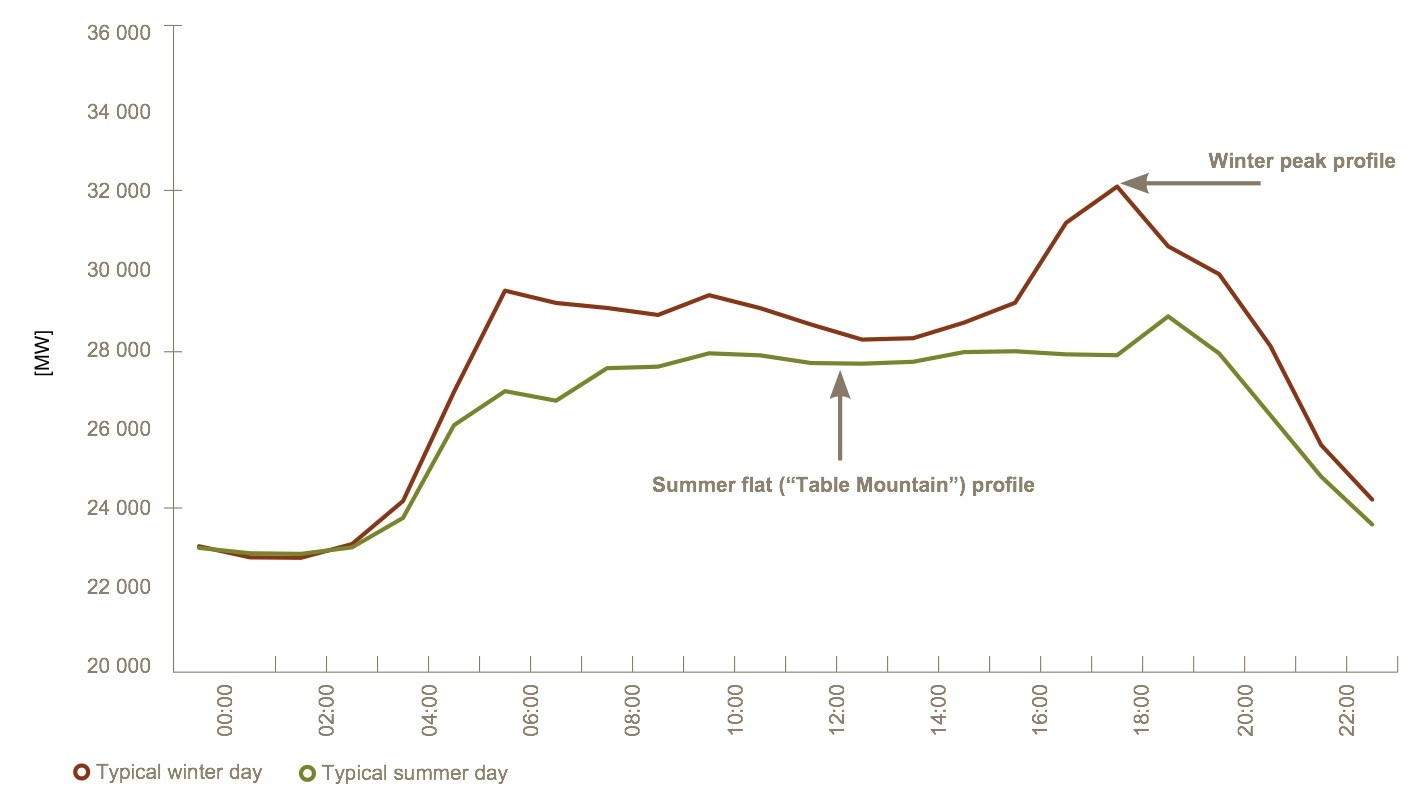
\includegraphics[width=0.9\linewidth]{FIG/SummerWinterDemand}
\caption[Summer and winter load profiles.]{Summer and winter load profiles \cite{Eskom2014}.}\label{DEMAND}
\end{figure}
\\
The demand in South Africa has different load profiles during winter and summer as shown in Figure~\ref{DEMAND}. The peak demand is usually in the evening hours and particularly high during winter time. According to Eskom is the peak demand at about 32~GW, while the usually demand during daytime is between 26~GW and 29~GW. \cite{Eskom2014}

\subsection{Rising energy consumption and security of supply}

\begin{figure}[!h] % Monthly Reserve
\centering
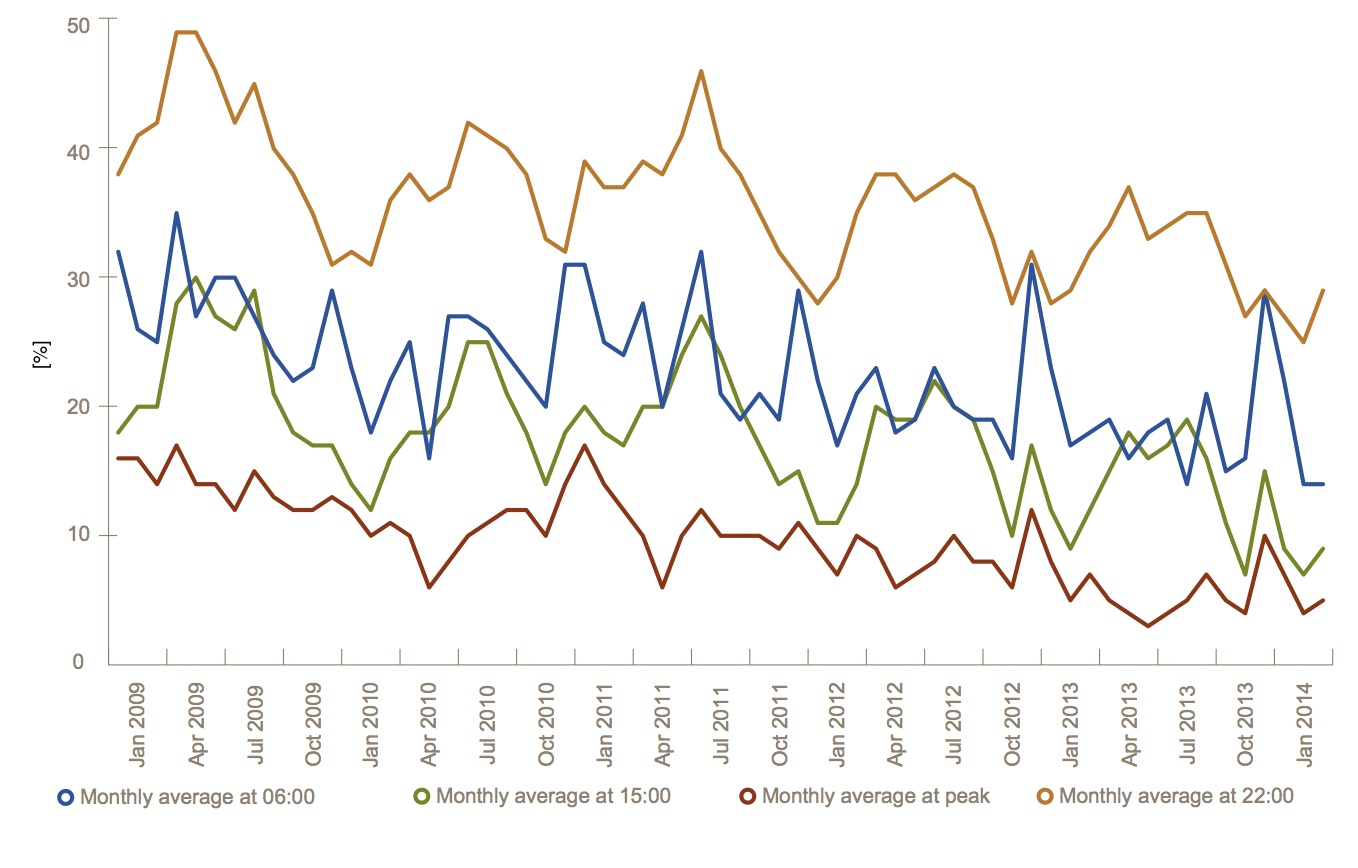
\includegraphics[width=0.9\linewidth]{FIG/AveragemonthlySA}
\caption[Average monthly \% operating reserves.]{Average monthly \% operating reserves\cite{Eskom2014}.}\label{Abb1}
\end{figure}


\begin{figure}[!h] % Demand growth
\centering
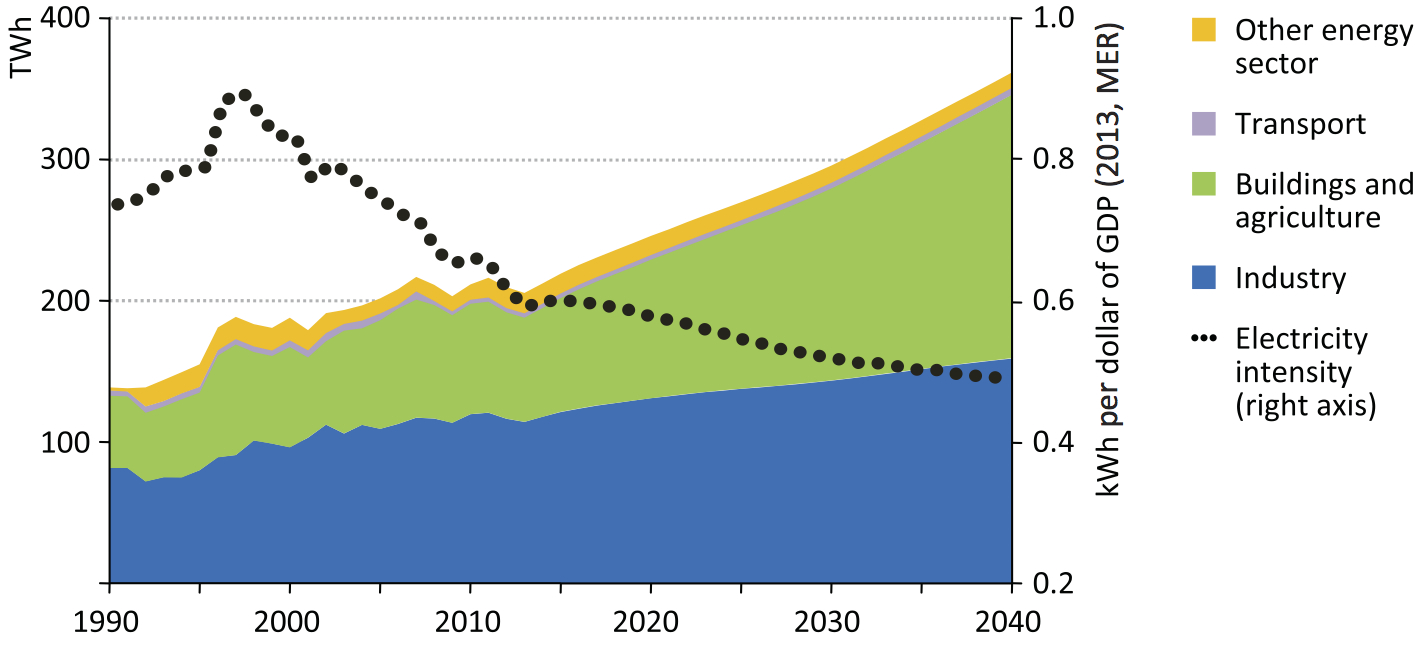
\includegraphics[width=0.9\linewidth]{FIG/SA_Electricity_demand_growth}
\caption[Electricity demand growth by sector in South Africa in the New Policies Scenario.]{Electricity demand growth by sector in South Africa in the New Policies Scenario \cite{IEA2014f}.}\label{Abb1}
\end{figure}

\subsection{Structure of power distribution}
Kilometerlängen, Verluste im Netz \cite{Eskom2014a}

On mainland sub-Saharan Africa, SA has with around 85~\% the highest electrification rate. About 11~\% of households don't have access to electricity and a further 4~\% rely on illegal access (non-paying) or obtain access informally (from one household to another but paying). \cite{IEA2014f}

\begin{figure}[htbp] % Netzstrucktur
\centering
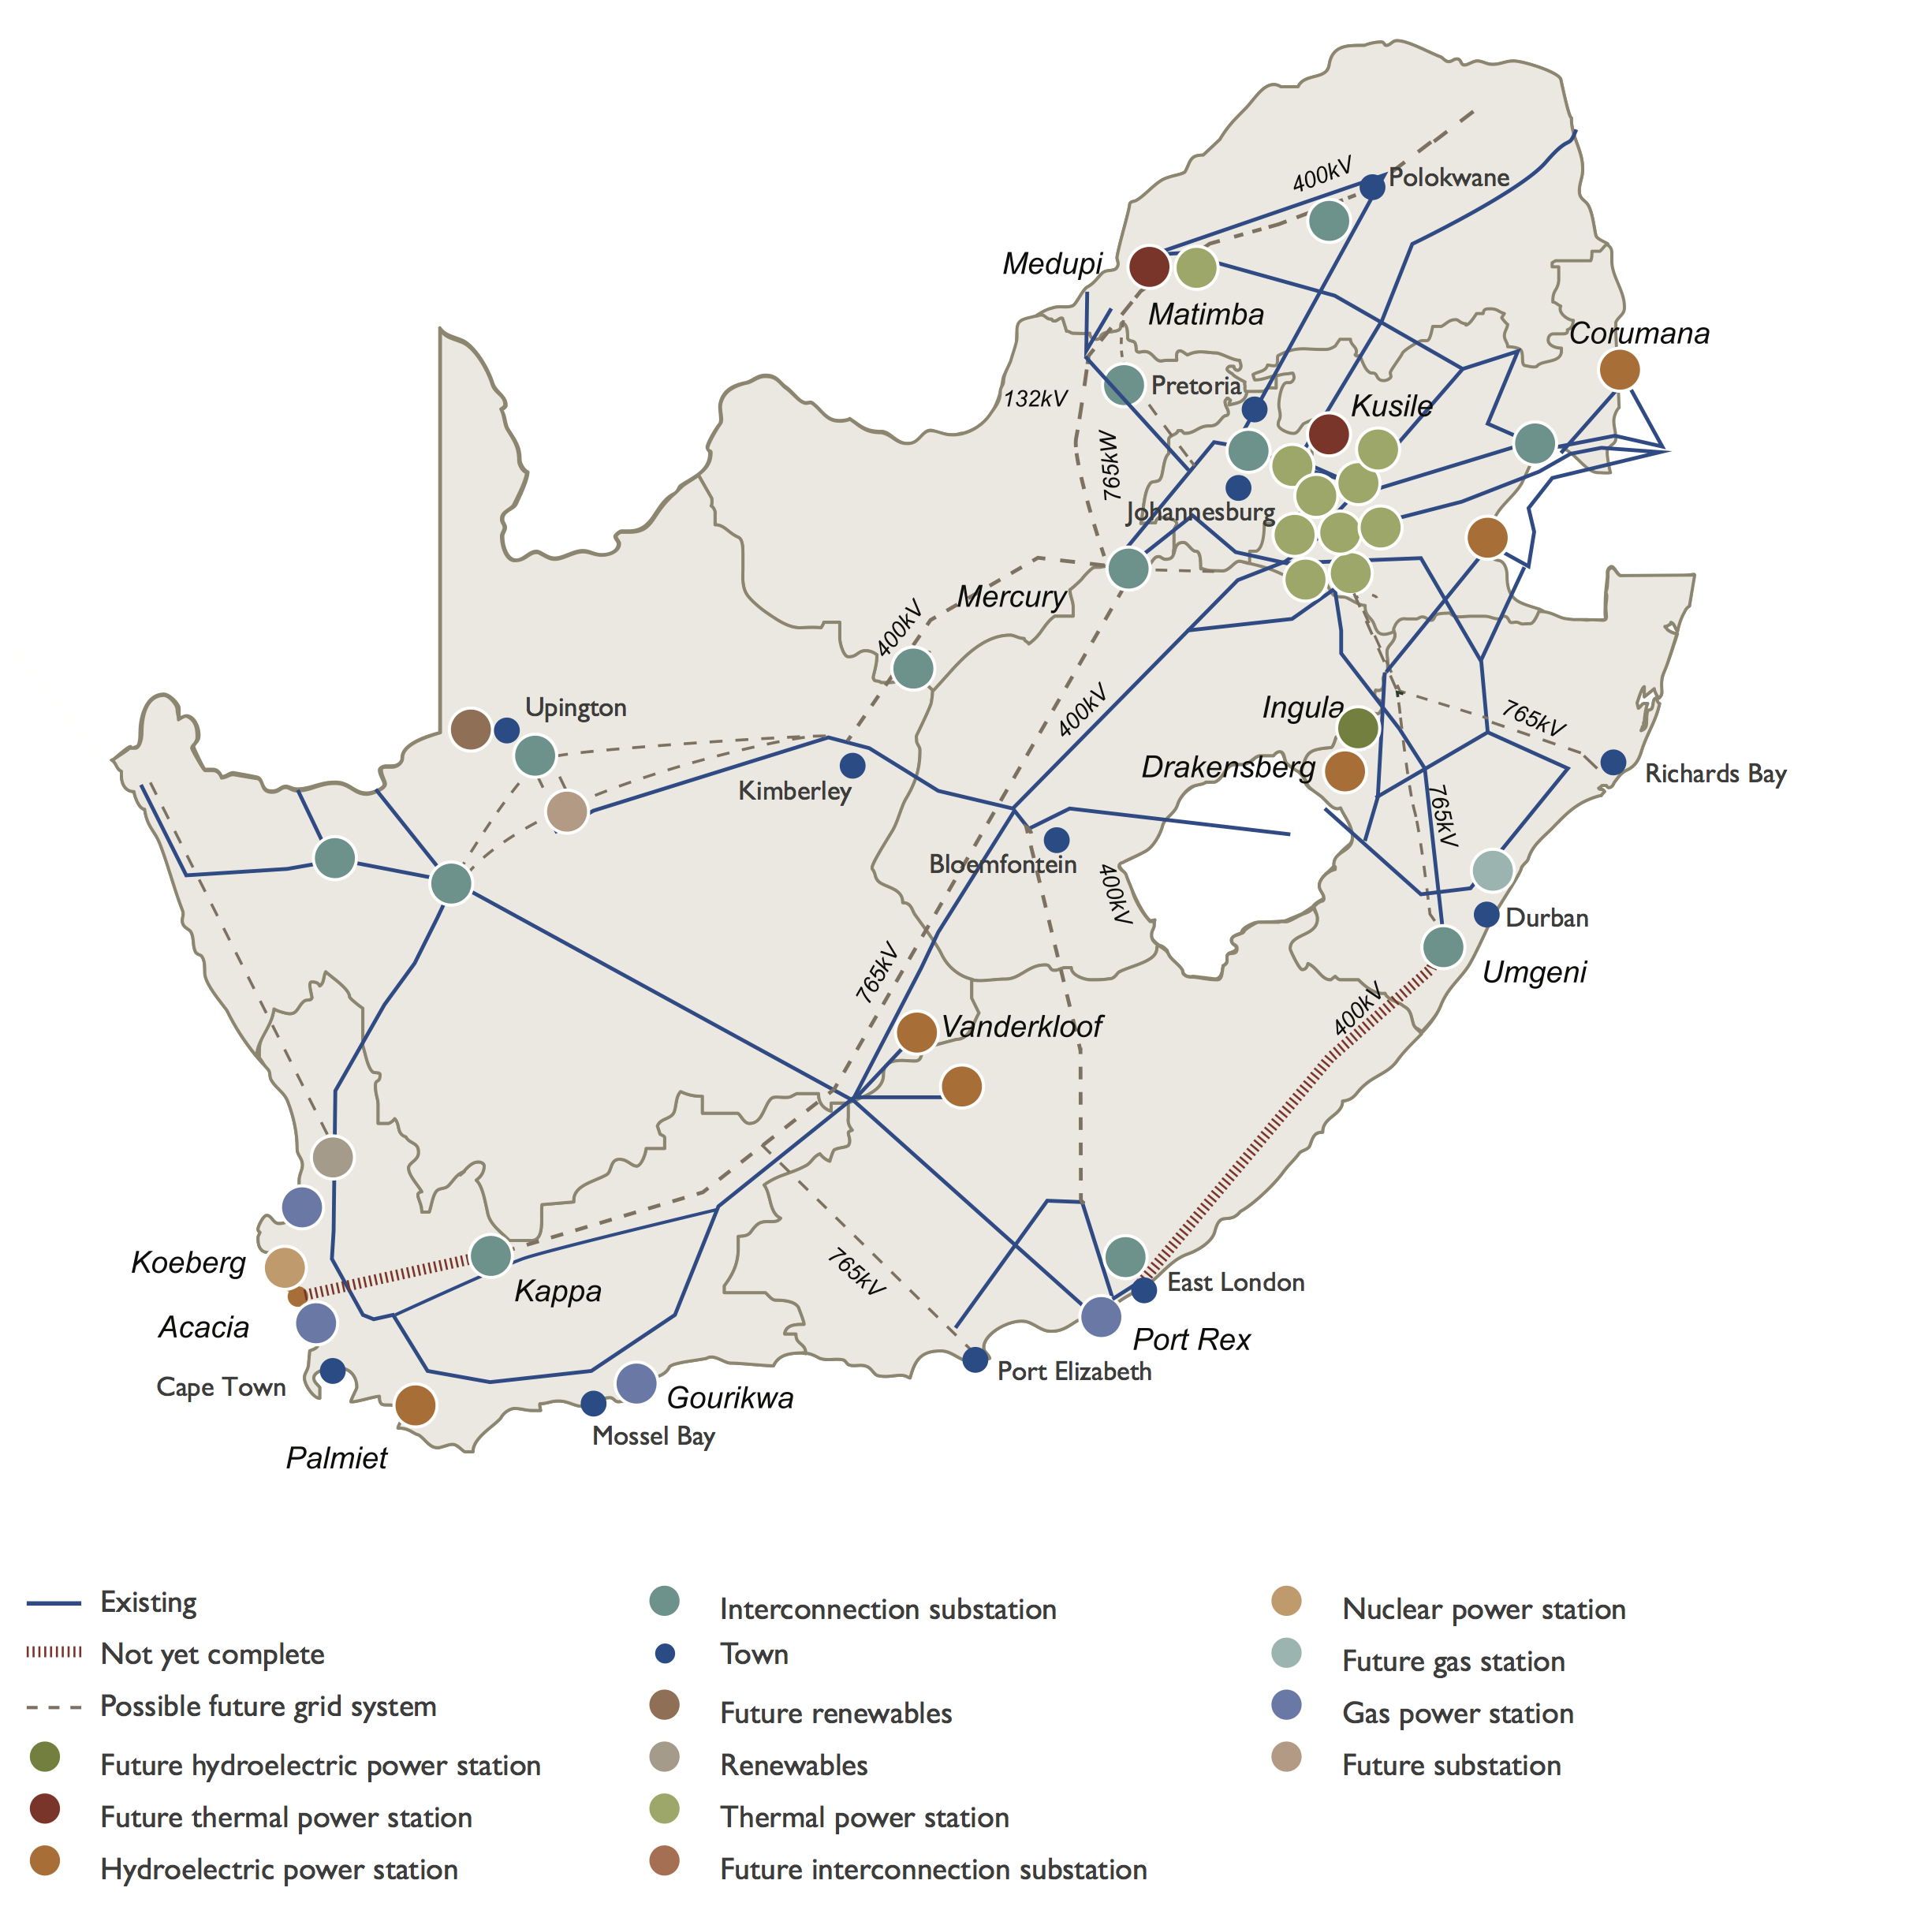
\includegraphics[width=0.9\linewidth]{FIG/transmissionprojekts}
\caption[Eskom’s transmission projects as at 31 March 2014.]{Eskom’s transmission projects as at 31 March 2014 \cite{Eskom2014}.}\label{Abb1}
\end{figure}

http://integratedreport.eskom.co.za/supplementary/app-transmission.php

\section{Renewable energy potential in South Africa}

\subsection{Energy outlook for South Africa}
Development of a Renewable Energy Power Supply Outlook 2015 for the Republic of South Africa
Achieved by Sebastian Giglmayr, BSc
\cite{Giglmayr2013}

\subsection{Government Incentives}

\section{Chapter summary}
\pagebreak
\chapter{Solar power in South Africa}\label{Solar power in South Africa}
South Africa is one of the country with the highest potential for generating solar thermal electricity in the word. Figure \ref{DHI-DIF} shows  the daily sum of global irradiation in Aberdeen, United Kingdom and Upington, South Africa. The yearly share of diffuse irradiation in Aberdeen overlaps 60 \%. In winter month the share reaches 90 \%. The share in Upington is approximately 25 \% and is in total significantly higher than Aberdeen. The direct comparison shows also the difference of the solar irradiation between northern and southern hemisphere during the year. It is obviously, that the seasons are the other way around between both hemispheres.\\
\\
This chapter shows energy impact from the sun and how it is distributed in SA. Furthermore the chapter comprised the current situation of solar power plants in SA.
\begin{figure}[h!] % DHI-DFI
\centering
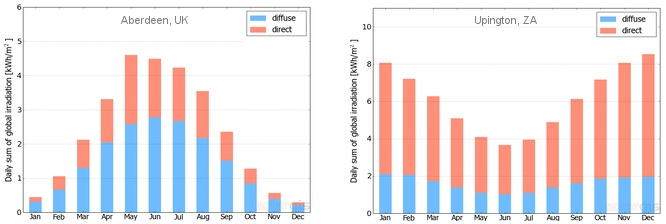
\includegraphics[width=1\linewidth]{FIG/DHI-DIF}
\caption[Long-term monthly variability of direct (DNI) and diffuse (DHI) irradiaton throughout the year for Aberdeen in the United Kingdom and Upington in South Africa.]{Long-term monthly variability of direct (DNI) and diffuse (DHI) irradiaton throughout the year for Aberdeen in the United Kingdom and Upington in South Africa \cite{SolarGIS2015}.}\label{DHI-DIF}
\end{figure} 
\section{Solar radiation}
The most important solar radiation parameters for designing a solar power plant are here defined:
\begin{itemize}
\item \textbf{GHI} (kWh/m\textsuperscript{2}/a or W/m\textsuperscript{2}): Global Horizontal Irradiance is the total amount of shortwave radiation received from above by a horizontal surface. It includes direct (beam) and a diffuse (scattered) irradiation. This value is of particular interest to PV or solar water heater with a fixed inclined angle.
\item \textbf{DNI} (kWh/m\textsuperscript{2}/a or W/m\textsuperscript{2}): Direct Normal Irradiance is the amount of solar radiation received per unit area by a surface that is always held perpendicular (or normal) to the rays that come in a straight line from the direction of the sun at its current position in the sky. Diffuse irradiation is totally excluded from the DNI. This quantity is of particular interest to  installations that track the position of the sun.
\item \textbf{DHI} (kWh/m\textsuperscript{2}/a or W/m\textsuperscript{2}): Diffuse Horizontal Irradiance is the amount of radiation received per unit area by a surface that does not arrive on a direct path from the sun, but has been scattered by molecules and particles in the atmosphere and comes equally from all directions.
\end{itemize}
Furthermore is irradiance understood as instantaneous density of solar radiation incident on a given surface, typically expressed in W/m\textsuperscript{2} and irradiation is the sum of irradiance over a time period expressed in J/m\textsuperscript{2} or more commonly used in Wh/m\textsuperscript{2}. The connection between the solar radiation parameters is shown in Equation \ref{GL_GHI}.The angle $\theta_\text{z}$ is the angle between the direction of the sun and the zenith (directly overhead).
\begin{align}
GHI=DNI*\cos(\theta_{z})+DHI \label{GL_GHI}
\end{align}
Figure\ref{irradiation} shows the solar GHI and the DNI data for the country. It is shown, that the ceiling value for GHI can be more than 2~300~kWh/m\textsuperscript{2}/a, whereas in some parts of the country the DNI  value attains about 2~900~kWh/m\textsuperscript{2}/a. This is significantly high than in the most regions worldwide, therefor SA is predestined for using solar technologies. The figure shows, that the southeastern coastline has predominantly the lowest irradiance values. The solar irradiation rise significant in the inland. The highest GHI can be find close to the Namibian boarder in the northeast of the country. The direct beam is also at highest in the western part of SA. The area around Springbok in the province Northern Cape has the highest DNI value of the country.
%% Abbildung GHI und DNI
\begin{figure}[h!]
        \centering
        \begin{subfigure}[b]{0.5\textwidth}
                \centering
                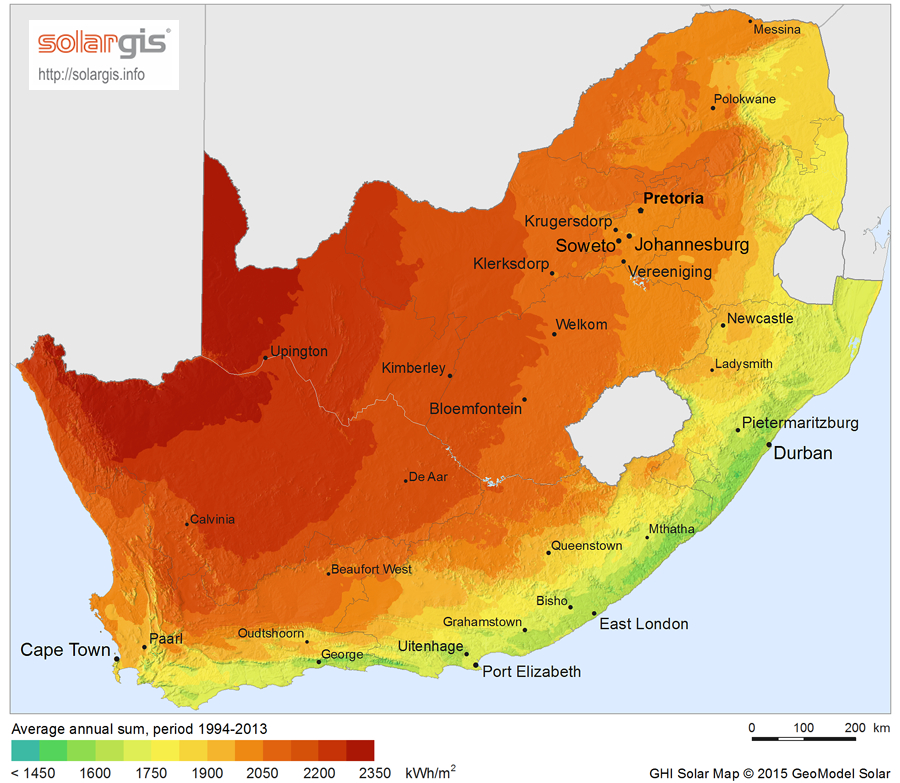
\includegraphics[width=0.95\textwidth]{FIG/SA_GHI}
                \caption{Global Horizontal Irradiation \cite{SolarGIS2015a}.}\label{fig:bild-links}
        \end{subfigure}%
        ~
        \begin{subfigure}[b]{0.5\textwidth}
                \centering
                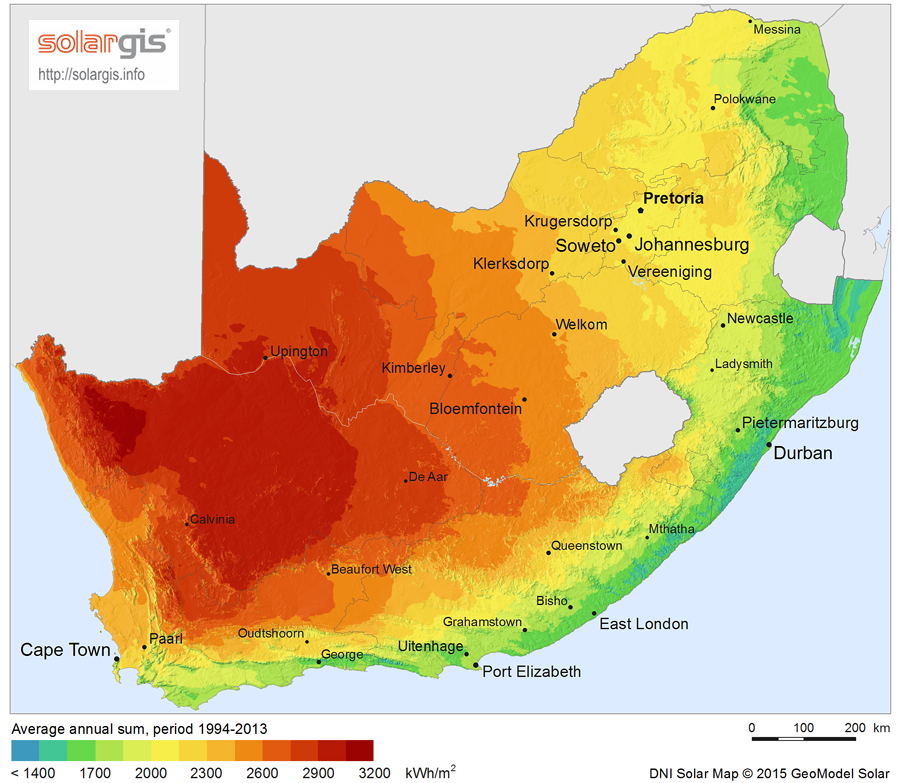
\includegraphics[width=0.95\textwidth]{FIG/SA_DNI}
                \caption{Direct Normal Irradiation \cite{SolarGIS2015b}.}\label{fig:bild-rechts}
        \end{subfigure}
        \caption{Solar radiation maps of South Africa.}\label{irradiation}
\end{figure}
\pagebreak
\section{Solar power plants in SA}
South Africa started there expansion in the field of solar power plants in the first round of the Renewable Energy Independent Power Producer Procurement Program (REIPPPP) in 2011. Now in 2015 starts the fourth round of the REIPPPP. Figure \ref{Solar-map} shows the allocation of all solar power plants of the REIPPPP. PV-power plants are marked in yellow and CSP-power plants are marked in orange. The numbers in the single marks expose in which REIPPPP-Round it belongs.
\begin{figure}[h!] % Solar-map
\centering
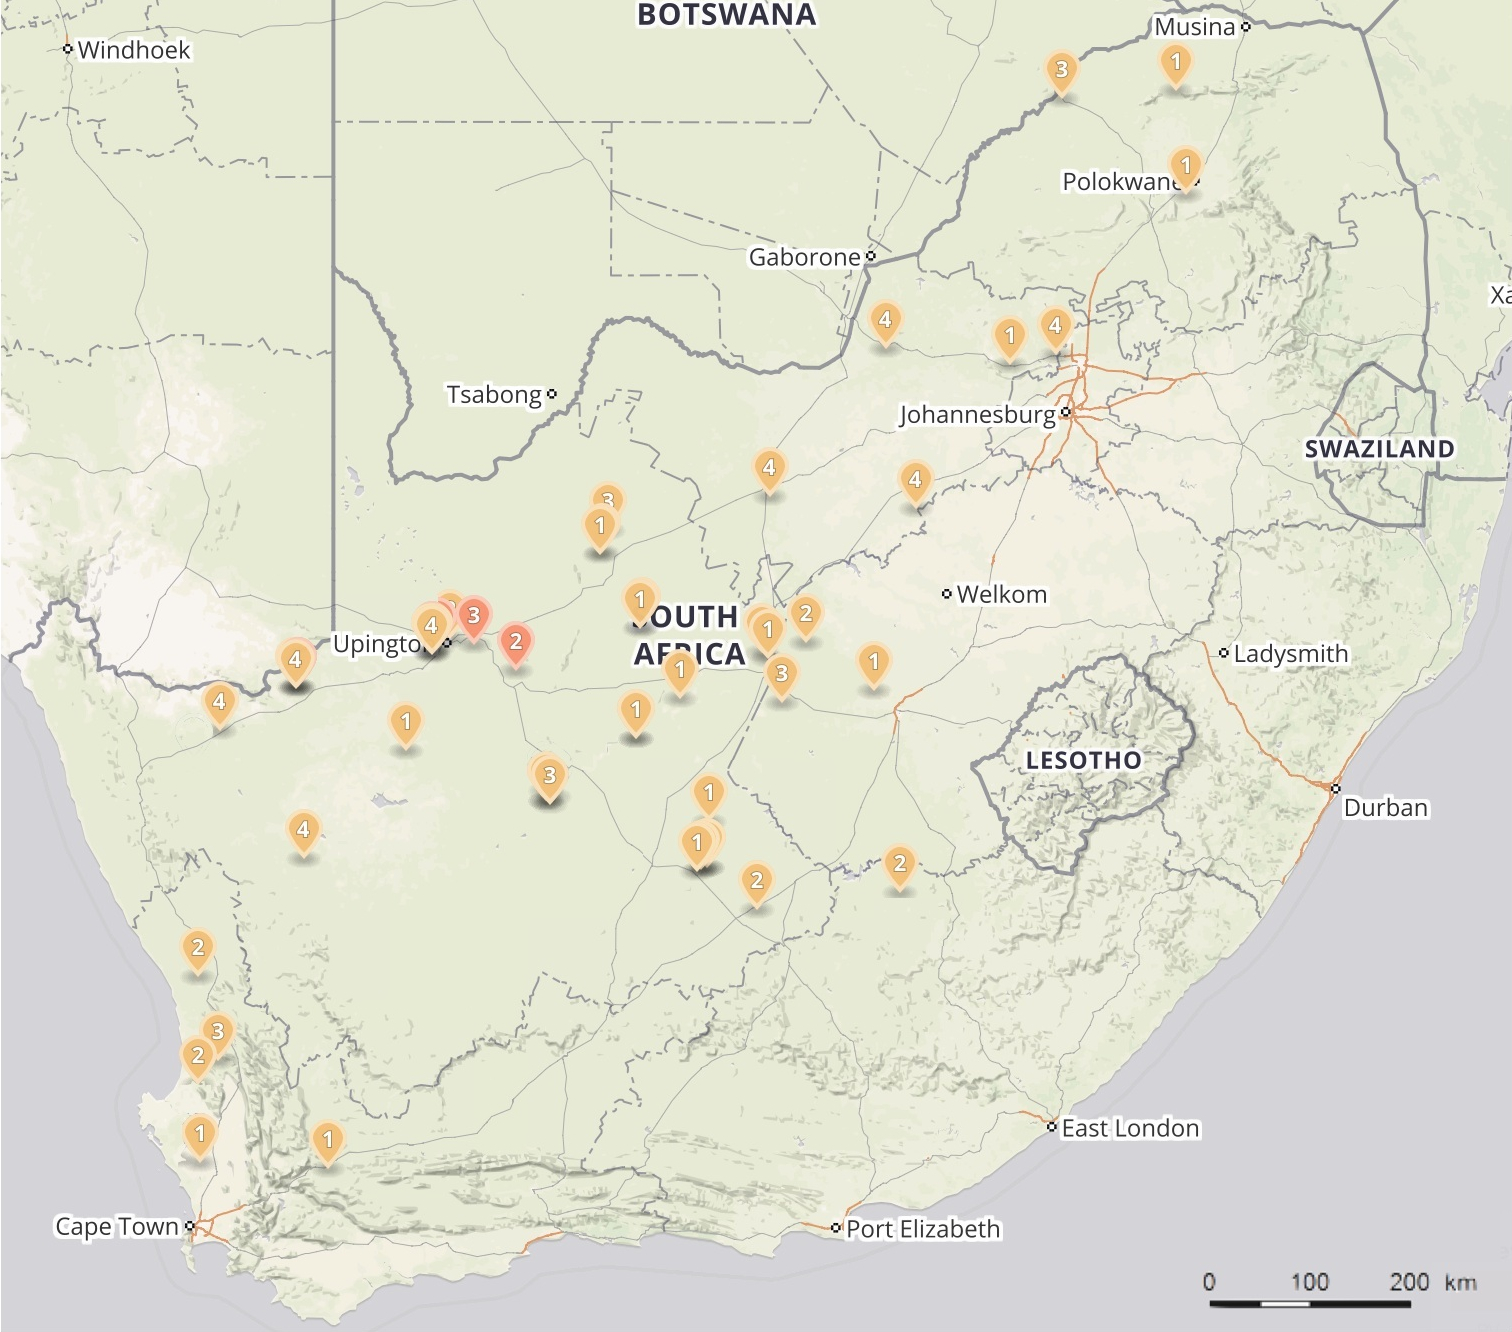
\includegraphics[width=1\linewidth]{FIG/Solar-map}
\caption[Allocation of all REIPPPP solar power plants in SA.]{Allocation of all REIPPPP solar power plants in SA \cite{Forder2015}.}\label{Solar-map}
\end{figure}\\
Currently SA has 26 fully operational PV-power plants with a total capacity of 1~048.7~MW, further seven PV-power plants with 135.35~MW are under construction, four more with 307.5~MW awaiting construction (approved \& financed) and there are six more PV-power plants in approvals, planning and financing with a total capacity of 415~MW. \\
Mainly PV-power plants are allocated in the Northern Cape. So 26 of 39 of the operational and planed plants are located there. Five more in the Western Cape, three each in the provinces Free State and Limpopo and each one in Eastern Cape and the North-West Province. \cite{Forder2015}\\
\\
"KaXu Solar One" is the first fully operational CSP-plant in SA and is shown in Figure \ref{KaXu-solar-field}. It is using parabolic trough technology and a 2.5~h thermal energy storage for generating of 100~MW capacity electricity. The CSP-plants "Khi Solar One" and "Bokpoort CSP Project" with a capacity of each 50~MW are under construction. Further three CSP-plants are awaiting construction, they have all a capacity of each 100~MW. \\
All six CSP-plants are located in the region around the cites to Upington or Pofadder in the Northern Cape. This region is predestined for CSP-plants, because it has high DNI (around~2~900~kWh/m\textsuperscript{2}/a) and a water connection through the Orange River. \cite{Forder2015}
\begin{figure}[!h]
\centering
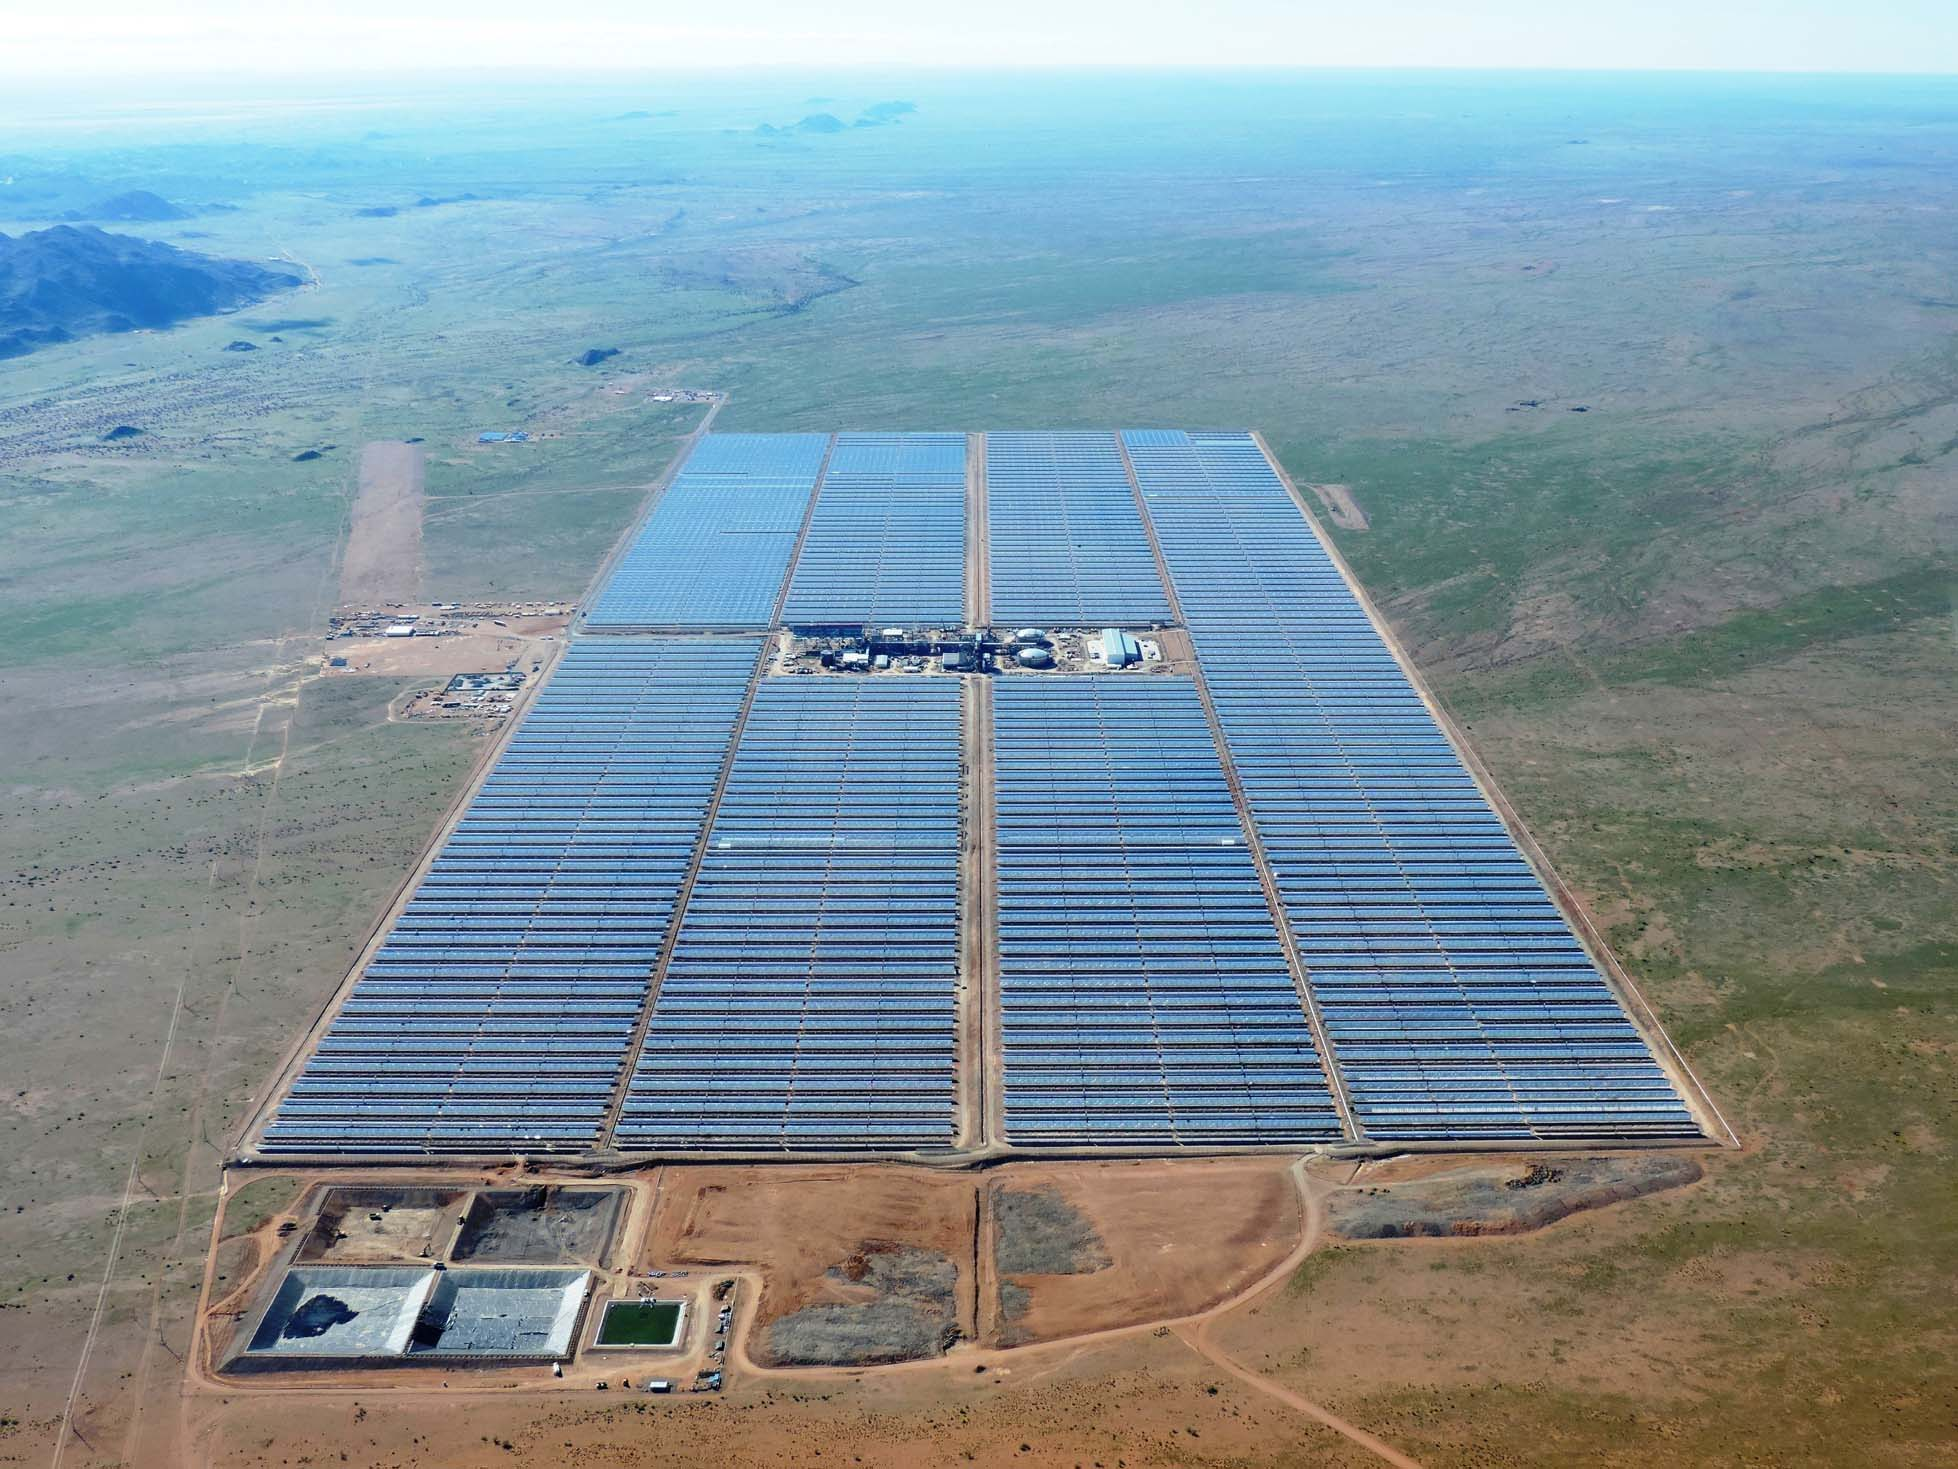
\includegraphics[width=1\linewidth]{FIG/KaXu-solar-field}
\caption[KaXu Solar One, a 100 MW parabolic trough plant with 2.5 hours of thermal storage in molten salts.]{KaXu Solar One, a 100 MW parabolic trough plant with 2.5 hours of thermal storage in molten salts \cite{AbengoaSolar2015}.}\label{KaXu-solar-field}
\end{figure}\\
\pagebreak
\chapter{Large scale solar power plants}
Almost all power that we use on our planet comes from the sun. Direct in form of radiation or indirect during wind, water and vegetation. Also the fossil power resources and reserves are stored energy from the sun in from of organic carbon compounds. There are two main technologies for generating electricity out of direct sun radiation. One is the direct conversion of solar irradiance to electrical energy while using photovoltaic. The other is to generate heat and convert it to electrical power. Figure~\ref{OverviewSTP} gives an abstract of the common technologies using direct solar power to generating electric power. This chapter has the focus on large-scale solar power plants and describes parts from both technologies.
\begin{figure}[!h] 
\centering
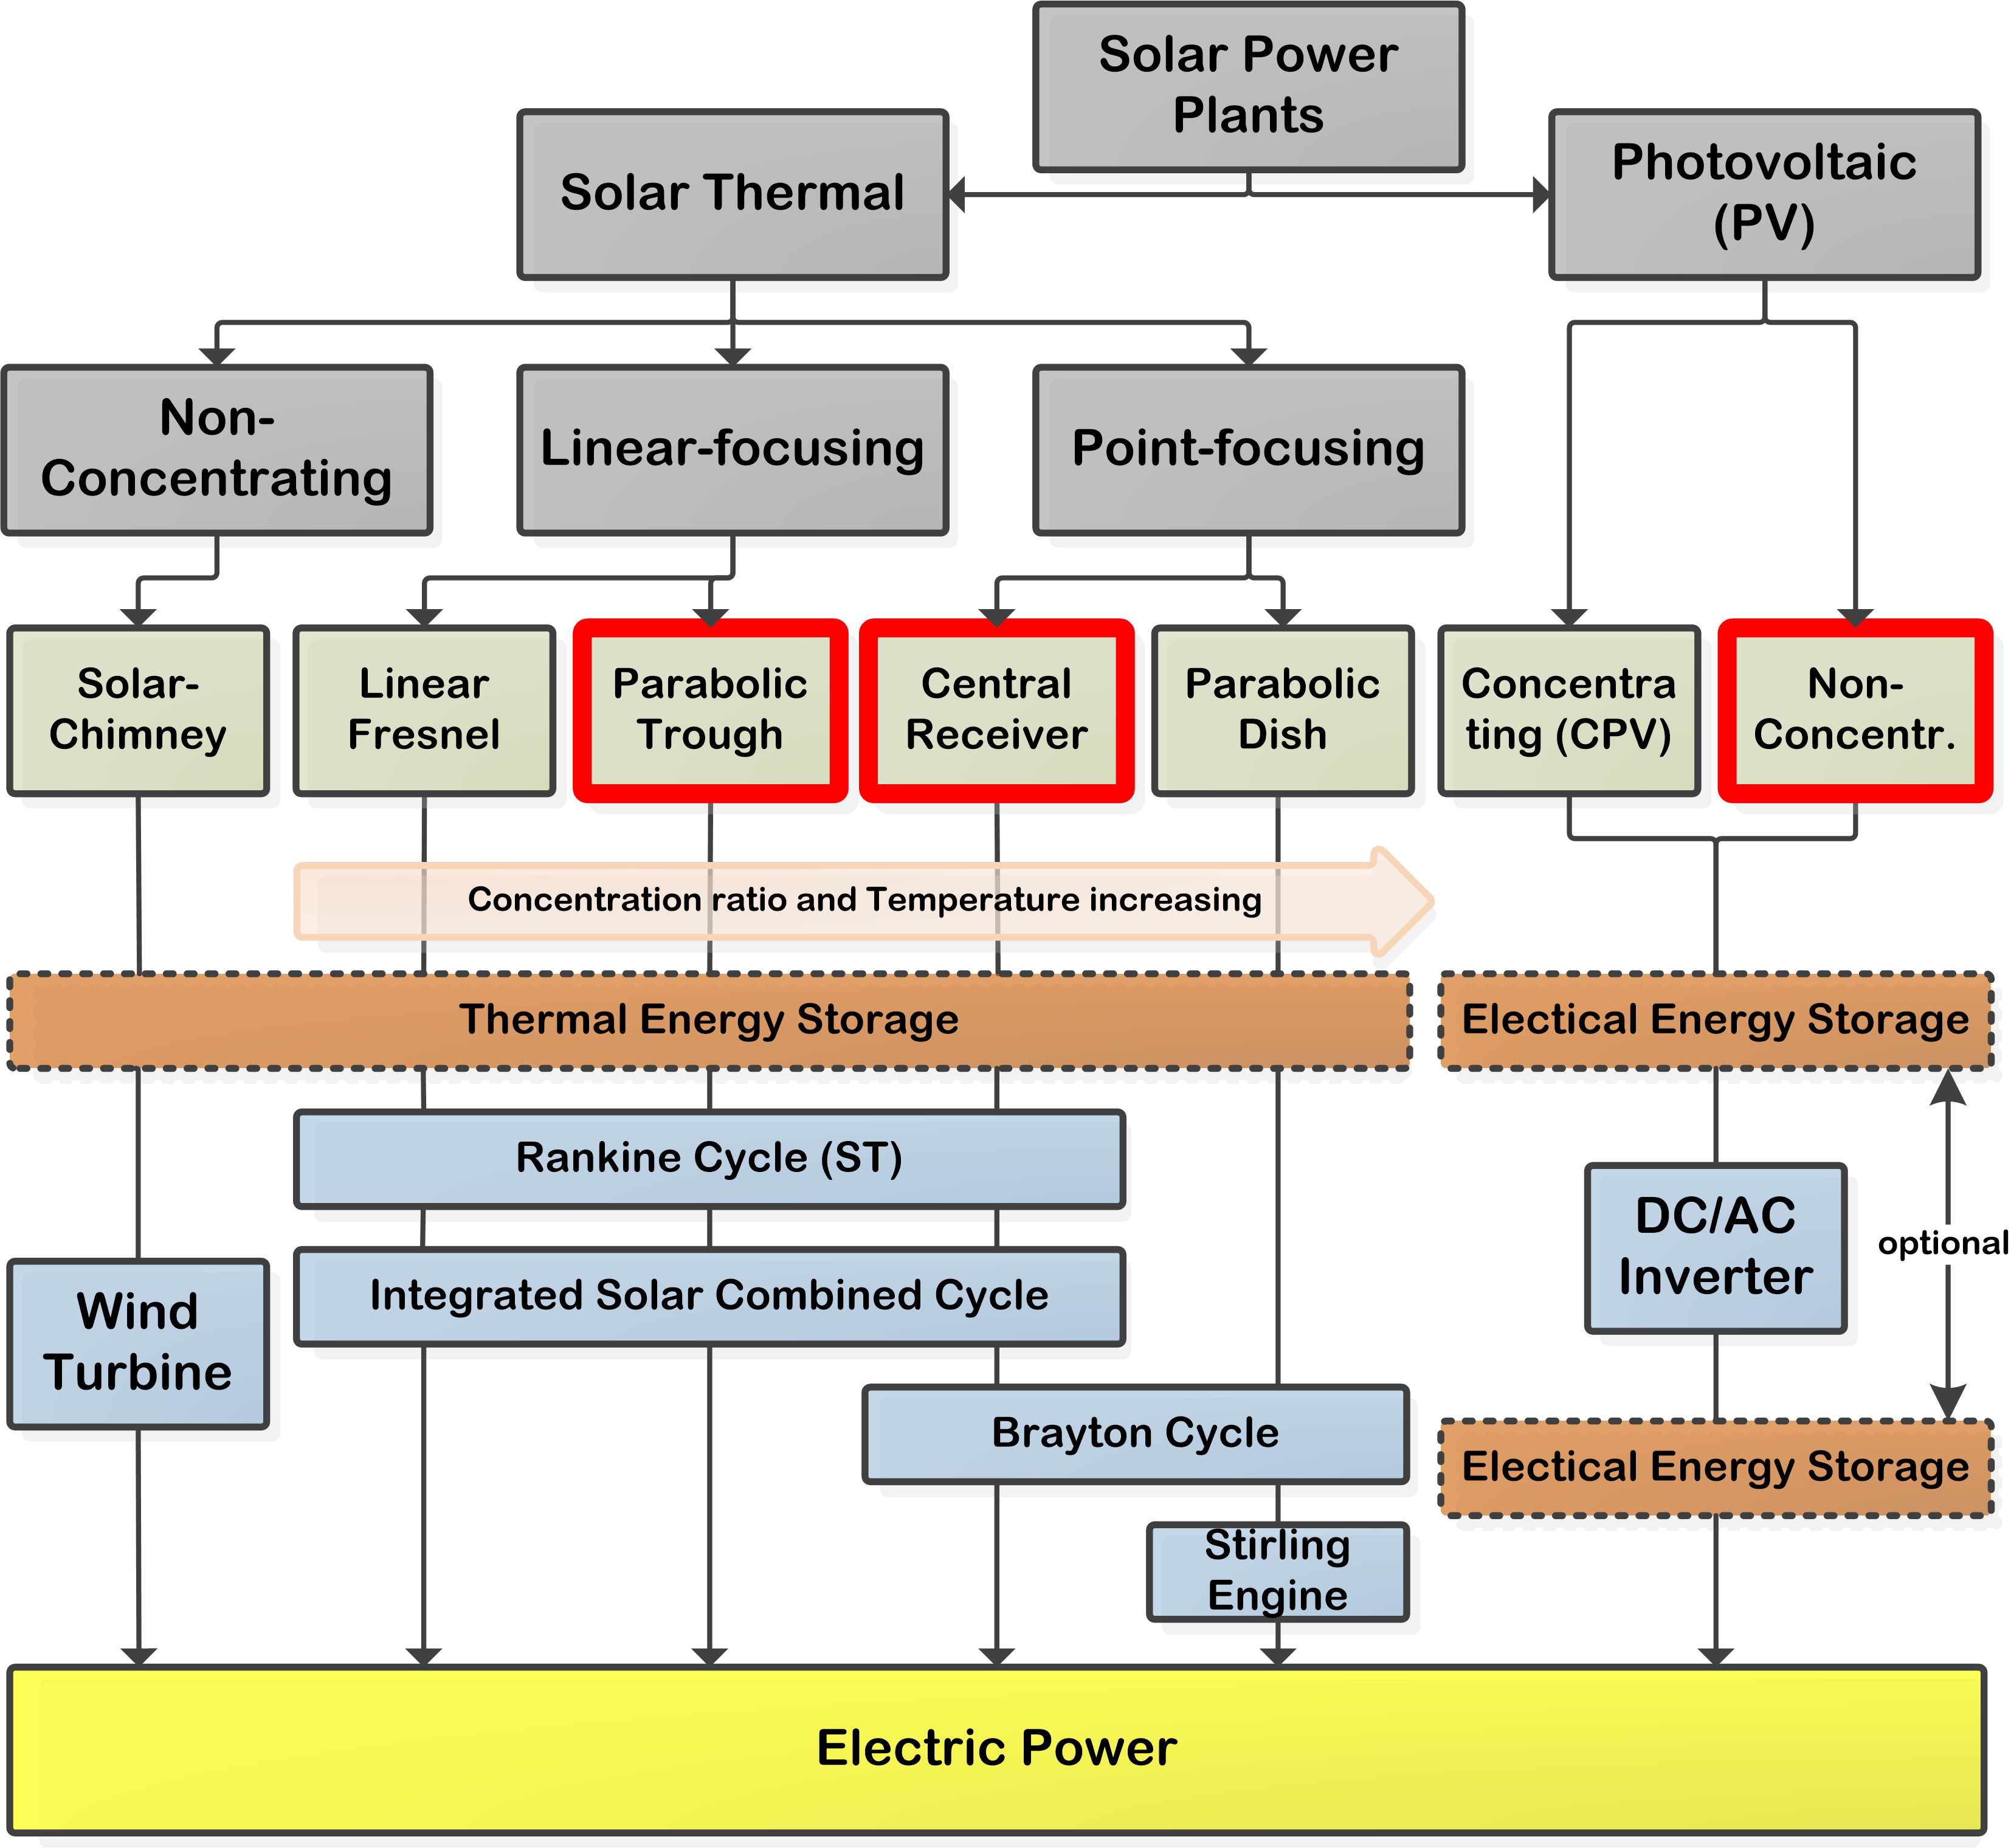
\includegraphics[width=0.75\linewidth]{FIG/OverviewSTP}
\caption[Overview of Solar Power Technologies.]{Overview of Solar Power Technologies.}\label{OverviewSTP}
\end{figure}
\\
Therefore it is split in the technology fields of large scale concentrated solar power plants (\ref{Large scale concentrated solar power (CSP) plants}) and large scale photo voltaic power plants (\ref{Large scale photo voltaic (PV) power plants}).
In detail the technologies with a large-scale power plant potential -- parabolic trough, central receiver and non-concentrating photovoltaic -- are described. Also the storage systems for both systems. 

\section{Large-scale CSP plants}\label{Large scale concentrated solar power (CSP) plants}
Concentrating solar power (CSP) systems use combinations of mirrors or lenses to concentrate direct beam solar radiation to produce forms of useful energy such as heat, electricity and others. This happens by use of various downstream technologies. Generally the CSP technology includes not only the concentrating solar thermal (CST) technology, but also concentrating photovoltaic (CPV) energy conversion. However, there is no focus on CPV in this thesis. That is why the term CST is put on a level with CSP.\\
A CSP plant comprises four main sub-systems: concentrating system, solar receiver, storage and power block. Also supplementary firing is used in some cases, but is basically not necessary nowadays. A graphic scheme of such a sub-system is shown in Figure~\ref{MainComp}. The separate components are linked together by energy flow in mostly radiation transfer or fluid transport. This chapter describes the function and gives an application overview of the individually components. 
\begin{figure}[!h] 
\centering
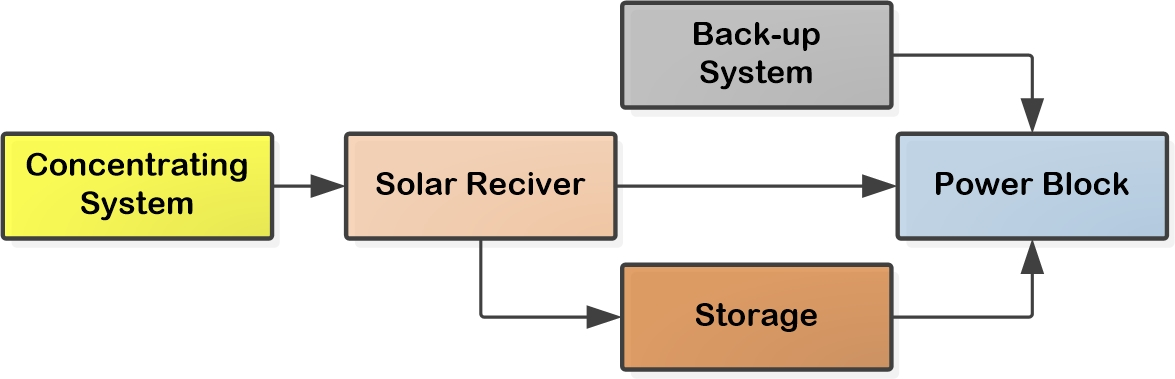
\includegraphics[width=0.85\linewidth]{FIG/MainComp}
\caption[Main components of a CSP plant.]{Main components of a CSP plant.}\label{MainComp}
\end{figure}
\\
The main advantage of CSP in opposite to other renewable energy producers is the thermal storage to provide power for cloudy days or during night time. Therefore the concentrating system and solar receiver have to produce more thermal energy then the power block can use directly. The ratio of the power capacity of the collector field to the capacity of the power block is defined as Solar multiple (SM). For CSP systems with storage, the number of hours of storage is based on the capacity of the power block. Chapter \ref{Subsection_storage_system} describes technical possibilities and application of thermal storage system for CSP.\\
\\
The solar receiver or concentrating system is eponymously for the main CST technologies. The two most common CSP plant technologies are parabolic trough collector (PTC) and central receiver (CR) systems (also known as solar power towers). Further types of CSP plant are linear Fresnel reflectors (LFR) and parabolic dish. The main difference of the technologies is the concentrating system. Thereof results the differences in optical design, shape of receiver, nature of the transfer fluid and capability to store heat before it is turned into electricity. In systems with a line focus (PTC trough and LFR) the mirrors track the sun along one axis. In those with a point focus (CR and parabolic dish), the mirrors track the sun along two axes. The receiver may be fixed, as in LFR and CR, or mobile as in PTC and parabolic dish systems. An overview of the technologies and there differences in relation to the focus and the receiver  is shown in Table \ref{tbl: CSPtech}.
\begin{table}[h!] % Main technologies 
  \centering
  \begin{tabular}{  m{5cm}  m{5cm}  m{5cm}  }
    \hline
    & \textbf{Line focus} & \textbf{Point focus} \\ 
    & Collectors track the sun along a single axis and focus irradiance on a linear receiver. This makes tracking the sun simpler. & Collectors track the sun along two axes and focus irradiance at a single point receiver. This allows for good receiver efficiency at higher temperatures.\\ \hline \hline
    \textbf{Fixed receiver} & &\\
    Fixed receivers are stationary devices that remain independent of the plant’s focusing device. This eases the transport of collected heat to the power block.
    &
    \begin{minipage}[t]{5cm}
      \centering
	 % 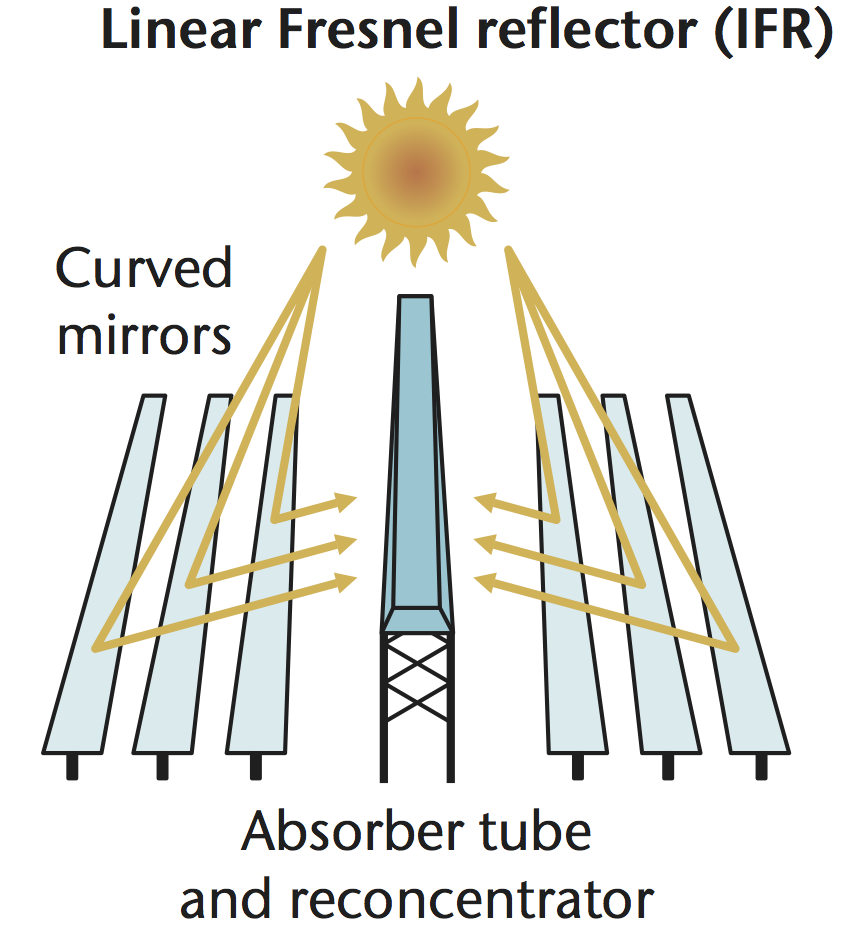
\includegraphics[height=55mm]{FIG/SUM/LF}
    \end{minipage}
    & 
    \begin{minipage}[t]{5cm}
      \centering
	 % 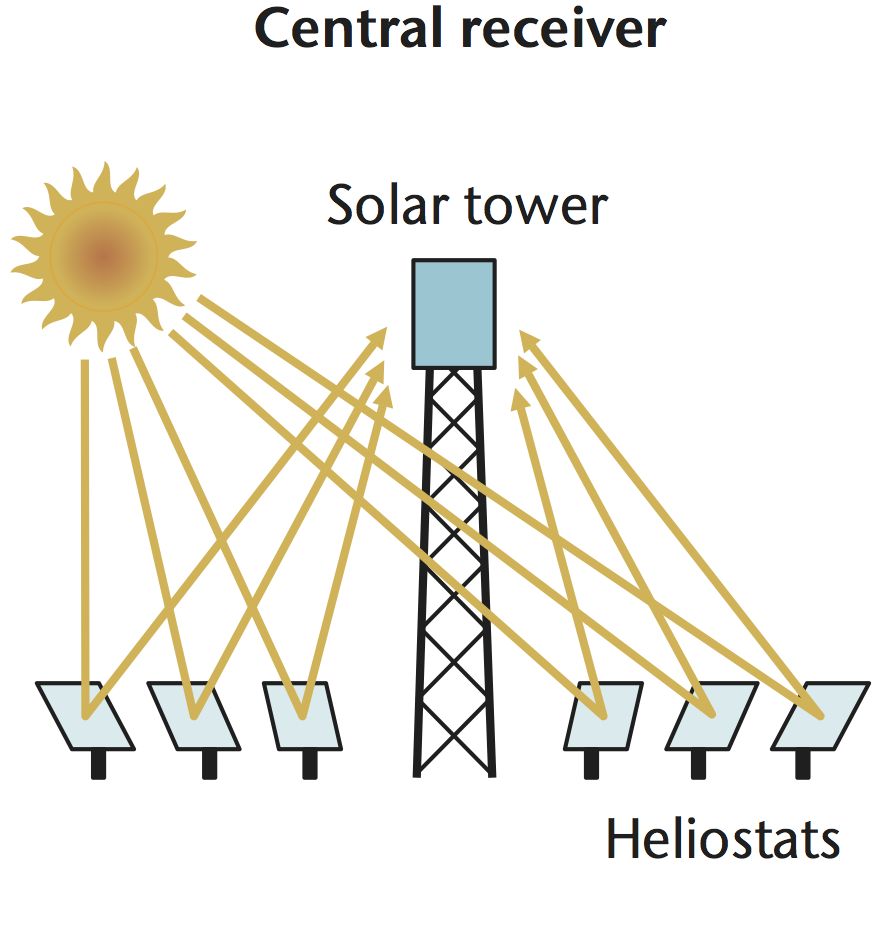
\includegraphics[height=55mm]{FIG/SUM/ST}
    \end{minipage}
    \\ \hline
    \textbf{Mobile receiver} & & \\
    Mobile receivers move together with the focusing device. In both line focus and point focus designs, mobile receivers collect more energy.
    &
    \begin{minipage}{5cm}
      \centering
	 % 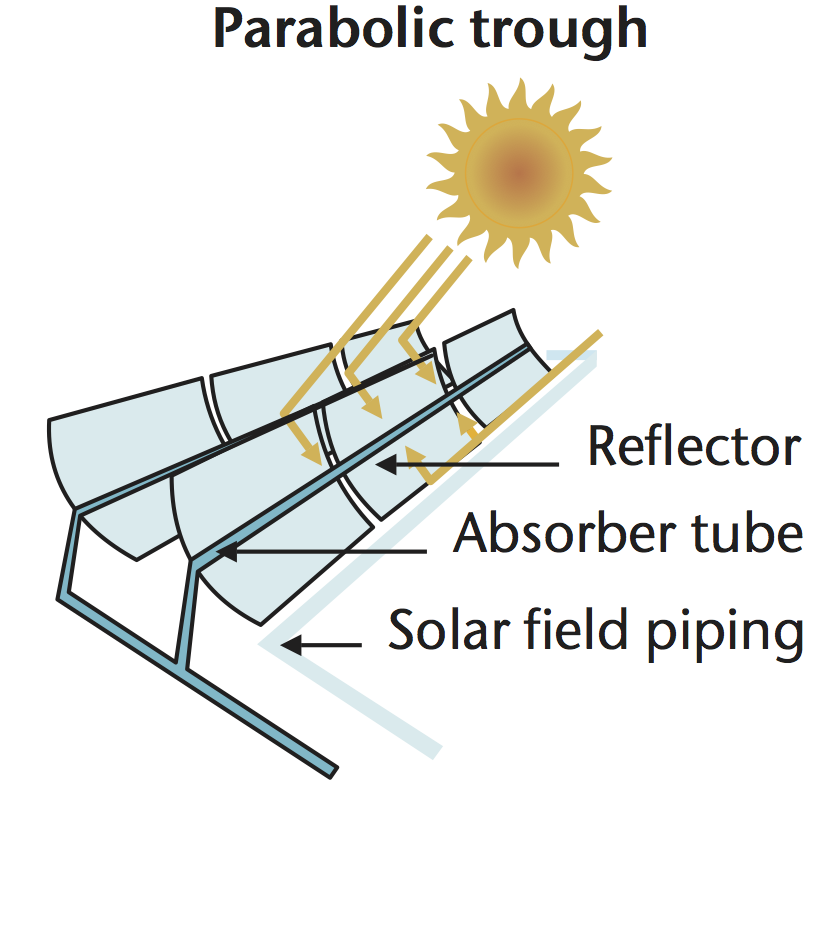
\includegraphics[height=55mm]{FIG/SUM/PT}
    \end{minipage}
    & 
    \begin{minipage}{5cm}
      \centering
	 % 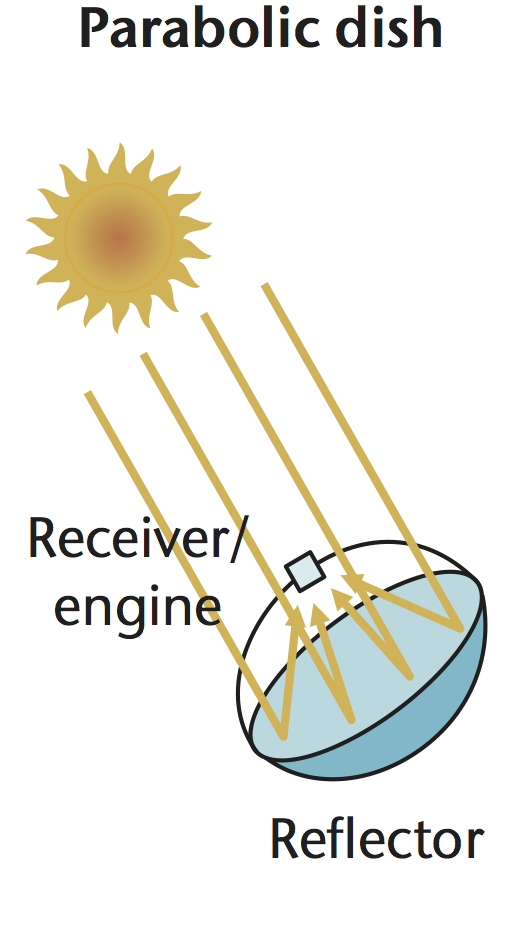
\includegraphics[height=55mm]{FIG/SUM/PD}
    \end{minipage}    
    \\ \hline
  \end{tabular}
  \caption[The main CSP technologies families.]{The main CSP technologies families \cite{IEA2014b}.}\label{tbl: CSPtech}
\end{table}
\\
As mentioned above is main difference between the CSP technology families how they concentrate the solar radiation. This strongly affects their overall efficiency. The parabolic dish has the best annual optical efficiency (about 90\%) because the concentrator axis is always parallel to the sun rays. The worst (about 50\%) is observed for linear Fresnel systems because of poor performance in the morning and in the evening. Intermediate values (65-75\%) are obtained for parabolic trough and tower systems. For each family the actual efficiency varies with the location, the time of day and the season of the year. \cite{EASAC2011} \\
\\
The capacity range of an CSP-plant is also strongly affected by the concentration ratio. The most common definition of concentration ratio is the ratio of the area of reflector aperture ($A_a$) to the area of receiver ($A_r$). The area concentration is:
\begin{align}
C=\frac{A_{a}}{A_{r}} \label{GL_concentration}
\end{align}
The concentration ratio from Equation \ref{GL_concentration} has an upper limit that depends on whether the concentration is a three dimensional (point focus) concentrator such as a parabolic dish and central receiver solar tower or a two-dimensional (linear focus) concentrator such as parabolic trough and linear Fresnel reflector. The maximum concentration ratio is based on the second law of thermodynamics applied to radiative heat exchange between the sun and the receiver. The maximum possible concentration ratio for circular concentrators is 45~000, and for linear concentrators is the maximum 212. \cite{Duffie2013}
\begin{table}[h!]  
  \centering
	\begin{tabular}{  p{3.0cm}  C{2.0cm}  C{2.2cm}  C{2.0cm}  C{2.0cm}  C{2.0cm}} 
\hline
\textbf{Technology} & \textbf{Capacity range} $(MW)$ & \textbf{Concent- ration} & \textbf{Peak system efficiency} $(\%)$ & \textbf{Annual system efficiency} $(\%)$ & \textbf{Thermal cycle efficiency} $(\%)$  \\ \hline \hline

Parabolic trough & 10-280$^1$ & 70-100 & 21 & 10-16 & 35-42 ST  \\ \hline
Fresnel reflector & 10-200 & 25-100 & 20 & 9-13 & 30-42 ST  \\ \hline
Solar tower & 10-200 &  300-1~000 & 23 & 8-23 & 0-45 ST  \\ \hline
Dish-Stirling & 0.01-0.4 & 1~000-3~000 & 29 & 16-28 & 30-40  \\ \hline
\multicolumn{2}{l}{ST = Steam Turbine}
\end{tabular}
\caption[Performance Characteristics of main CSP technologies families.]{Performance Characteristics of main CSP technologies families \cite{Pitz-Paal.2013} \cite{AbengoaSolar2013a}$^1$.}\label{tbl: CSPCharacteristics}
\end{table}
\\
But actually the technical implementation of concentration ratio is the main parameter for the capacity range of a CSP plant. Table~\ref{tbl: CSPCharacteristics} gives an overview of some of the performance characteristics of the concentrating solar power concepts. More details are listed in Annexure I, Part A, Figure~\ref{CSPOverview1} on Page~\pageref{CSPOverview1} and Figure~\ref{CSPOverview2} on Page~\pageref{CSPOverview2}. PTC, LFR, and CR can be coupled to steam cycles of 10-280~MW electric capacity (and more), with thermal cycle efficiencies of 30-45~\%. Also the applies for stirling engines which are coupled to dish systems have similar efficiency ranges. The conversion efficiency of the power block remains essentially the same as in conventional-fired power plants. The annual system efficiency are the net power generation over incident beam radiation. They are lower than the conversion efficiencies of conventional steam or combined cycles, because they include the conversion of solar radiative energy to heat within the collector and the conversion of the heat to electricity in the power block. \cite{Pitz-Paal.2013}\\
\begin{figure}[!h] 
\centering
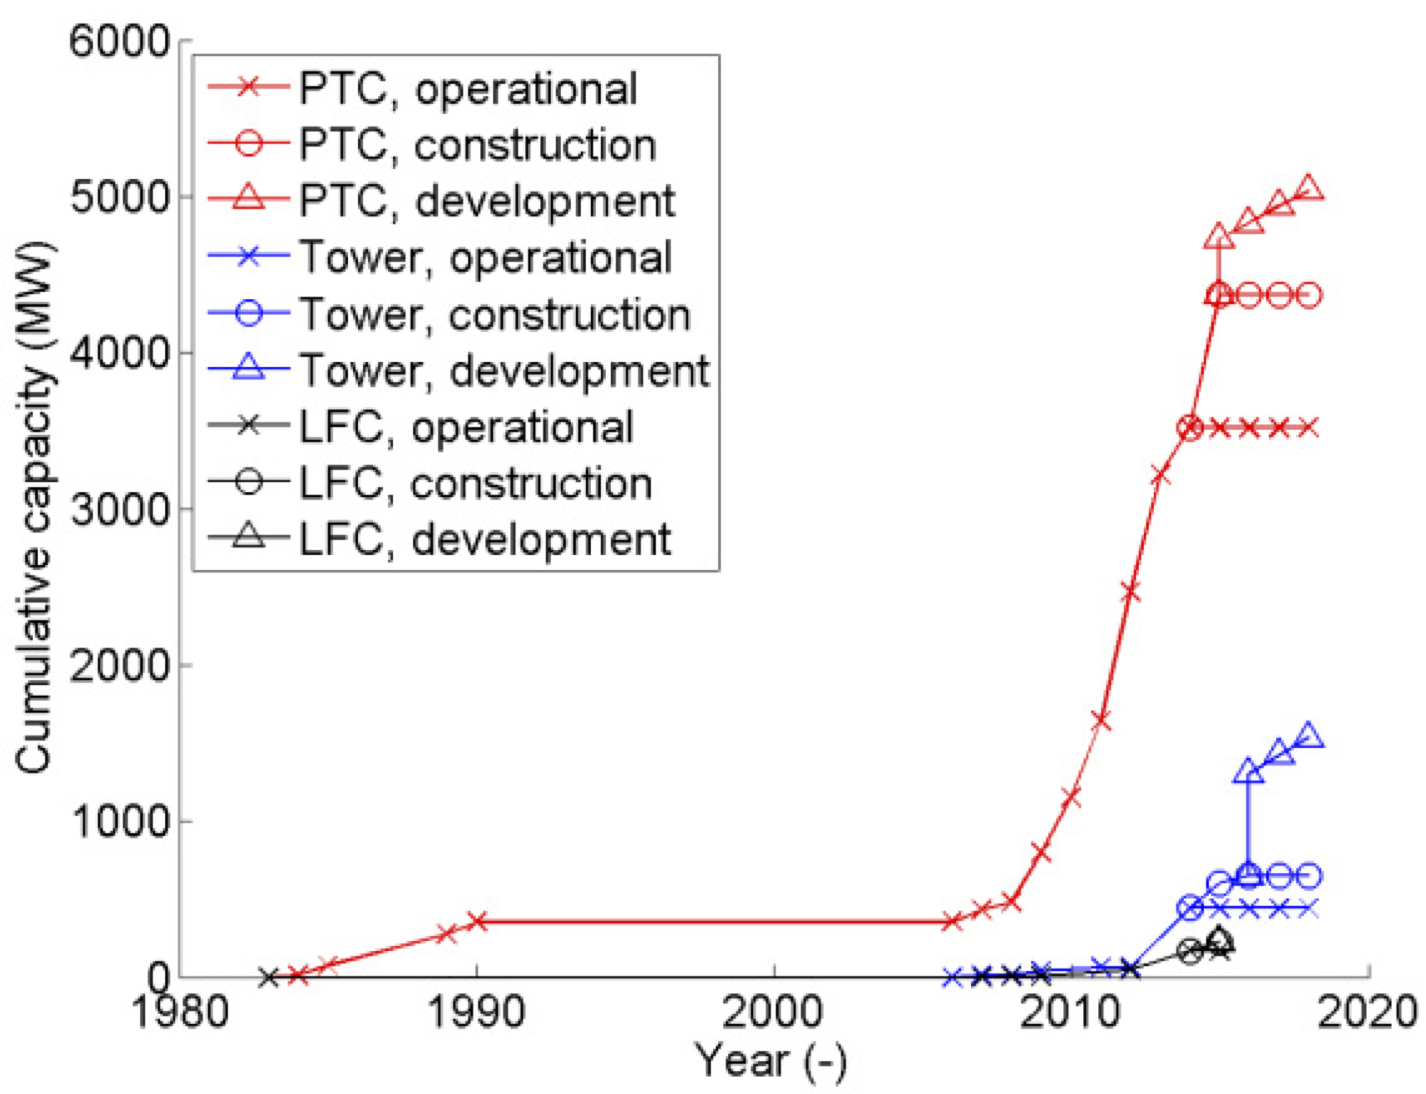
\includegraphics[width=0.65\linewidth]{FIG/CSP_technology_development}
\caption[Historical development of CSP technologies.]{Historical development of CSP technologies \cite{Abbas2015}.}\label{CSP_technology_development}
\end{figure}\\
The development of the actual CSP plant technology goes back in the 1970's and 1980's, which is a consequent from the first two Oil crises. Figure~\ref{CSP_technology_development} shows the historical development of PTC, LFR in the Figure called linear Fresnel collector (LFC) and the CR (tower). The parabolic dishes have not succeeded at all and aren't shown here. The reason for that is mainly due to the high structural costs of moving an large diameter dish with two-axes tracking. One might observe that the predominant technology is the PTC, with an installed capacity well above 3~GW. CR have started the exponential development some years later compared to PTC, which explains why the operational installed capacity is much lower. Similarly the development for LFR have started even later, which drives to the lowest installed capacity of the three technologies. The difference in the timing of the three successful technologies is very influenced by the CSP development in its first golden period, the 1980's. In such period important central tower prototypes were built in USA (Solar One, Solar Two, CESA-1) and a 365~MW PTC solar plant was installed in the Mojave Desert. When the oil prices dropped at the end of the second oil crises interest on renewable energies was lost until the last decade. \\
\\
With regard to the past development in the different CSP technology dealt the following chapters with the PTC (\ref{subsection_PTC}) as well as with the solar tower technology (\ref{subsection_CRS}). The necessary concepts of the storage systems (\ref{Subsection_storage_system}) and an overview of common heat transfer fluids (\ref{subsection_HTF}) are also included. The systems for the converting thermal to electrical power will be also summarized (\ref{subsection_powerblock}).  Parabolic dishes and LFC are not further considered depending to the development stage.
\pagebreak
\subsection{Parabolic-trough concentrating solar power} \label{subsection_PTC}
Parabolic trough power plants consist of many parabolic-trough-shaped concentrator that reflects direct solar radiation onto a receiver or absorber tube (also called receiver tube) located in the focal line of the parabola. The heated fluid is used in a steam generation system, to drive a steam turbine/generator cycle. Optional thermal storage and/or fossil-fired backup systems are possible. A schematic concept of a parabolic trough power plant is shown in Figure \ref{parabolic_troughs}. The collector field is made up of a large number of single-axis-tracking parabolic trough solar collectors and receivers. The solar field is modular in nature and comprises many parallel rows of solar collectors, normally aligned on a north-south horizontal axis. The collectors track the sun from east to west during the day to ensure that the sun is continuously focused on the linear absorber tube.
\begin{figure}[!h] 
\centering
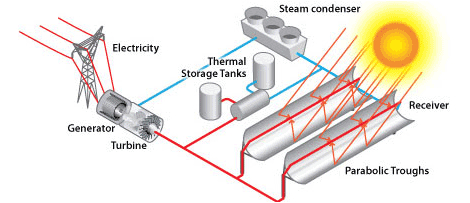
\includegraphics[width=0.7\linewidth]{FIG/parabolic_troughs}
\caption[Schematic parabolic trough power plant concept.]{Schematic parabolic trough power plant concept \cite{U.S.DOE2013}.}\label{parabolic_troughs}
\end{figure}
\\
The first graphically documented parabolic-trough solar collector was designed and built in 1870 by Swedish engineer John Ericsson. This collector produced 373~W by a steam engine had and had a solar radiation collecting surface of 3.25~m$^2$. \cite{Fernandez-Garcia2010}\\
Current PTC are based on developments in the united states which began after the first oil crisis. In the 1980s the first commercial used PTC plants was build. Most outstanding the implementation of the nine SEGS (Solar Electricity Generating System) plants. Build from 1984 (SEGS-I) to 1990 (SEGS-IX) in the Mohave Desert (California, USA) by LUZ International Limited and still operating. In total they have an electrical output of 354 MW and more than two million square meters of parabolic-trough collectors. They using oil to produce steam in heat exchangers before being circulated back to the solar field. Like in a electricity generating plant the steam is used in a conventional steam turbine. After the cutting down of government incentives for renewable systems and the oil price fell again in the 1980s the installation of more SEGS plants went unfeasible. \cite{Kalogirou2014a}\\
But the technology is still applied in most of the present build commercial parabolic trough power plants. Today they are using as HTF synthetic oil, typically out of biphenyl/diphenyl oxide fluid. The maximum cycle temperature is limited to values below 400$\,^{\circ}\mathrm{C}$ in order to avoid decomposition of the HTF. The thermal energy from the solar field is transported by the HTF to the heat-exchanger steam generator systems providing the superheated steam for the turbine of typically 370-380$\,^{\circ}\mathrm{C}$. The limitation of the upper process temperature to about 400$\,^{\circ}\mathrm{C}$ can be overcome by changing the HTF. A higher process temperature leads to a significant increase in the thermodynamic conversion cycle efficiency. A summary of current applied HTFs can be found in Chapter~\ref{subsection_HTF}.\\
An alternative HTF is water/steam, which is used in the steam cycle any way. The direct steam generation (DSG) in parabolic trough collectors demonstration loops steam reaches temperature of 550$\,^{\circ}\mathrm{C}$. Aside from the process temperature, the benefits of DSG compared with oil are based on savings in the heat exchanger, in reduced pumping effort, and the uncritical handing of the medium. But there are still barriers for commercial scale application. Some of the most important technological challenges of the DSG parabolic trough plant are the control stability, receiver tube viability, and collector interconnection feasibility.  \cite{Alguacil2014}\\
Another alternative HTF for PTC is molten salt. Salts already proved there competence in solar tower power plants and also application of liquid salts in parabolic trough systems have been investigated. Salts has suitable thermophysical properties, namely high boiling and decomposition point, low vapor pressure, high specific heat capacity, high thermal conductivity, and high density at low pressures \cite{Cordaro2011}. Molten salt has also the advantage to be the art of science in thermal storage for large- scale CSP plants (see Chapter \ref{Subsection_storage_system}).  Furthermore, typical salt mixtures are significantly cheaper than synthetic oils \cite{Gil2010}. The 5~MW Archimede commercial PTC plant is using a mixture of sodium nitrate (60\%) and potassium (40\%) nitrate since 2010 \cite{NREL2012}. The upper solar-field outlet temperature is 550$\,^{\circ}\mathrm{C}$ but starts crystallization of the non-eutectic melt occurs at 238$\,^{\circ}\mathrm{C}$ \cite{Cordaro2011}. That is one concerns with molten salt-based parabolic trough plants. The solar plant needs to be fully equipped with impedance and trace heating systems in order to ensure non-freezing of the salt. Therefore also the the process setup needs to be modified. But according to the researcher of the "Archimede Solar Energy molten salt parabolic trough demo plant" the molten salt parabolic trough (MSPT) technology is mature for large scale commercial applications without any critical points to be addressed \cite{Maccari2015}. Also the higher investment costs in solar field and piping, as well as maintenance and operation cost seams to be manageable and will be overcome to the increase in total plant efficiency and lower storage and HTF costs. Therefore the expected levelized cost of electricity (LCoE) of PTC power plants will decrease around 20\% \cite{Richert2015}. Component manufacturers are starting to introduce products specifically aimed at this technology. Upcoming projects needs to validate this expected decrease of LCoE in commercial scale and represent their profitability. \\ 
\\
As mentioned above a PTC power plant consists out of the components collector and receiver, which held together by support structure. This components are connected in loops, which building the solar field.
\subsubsection{Parabolic Trough Collectors}
The task of PTC module is to reflect the radiation of the sun accurately to the receiver tube. So the main components of a PTC module are actually the curved mirror and the absorber tube. But usually the PTC means the reflector and its support structure. The absorber tubes are separately regarded. The structure holds the components in place and connects the reflector modules between each other. To concentrate the radiation to the absorber tube the shape of the reflective surface is in parabolic form like in Figure \ref{PTC_section}. There shown is a section of a PTC with the dimensions of the commercial used LS-3, EuroTrough and Senertrough-1 and their focus point. This focus point is only at this position when the z-axis is in the direction of the Sun. Therefor the PTC is controlled by means of astronomical calculations, often supplemented by a Sun position sensor. The absorber tubes mounted in the focal line move with the collector and are connected to the stationary field piping via flexible hoses or rotating joint arrangements.
\begin{figure}[!h] 
\centering
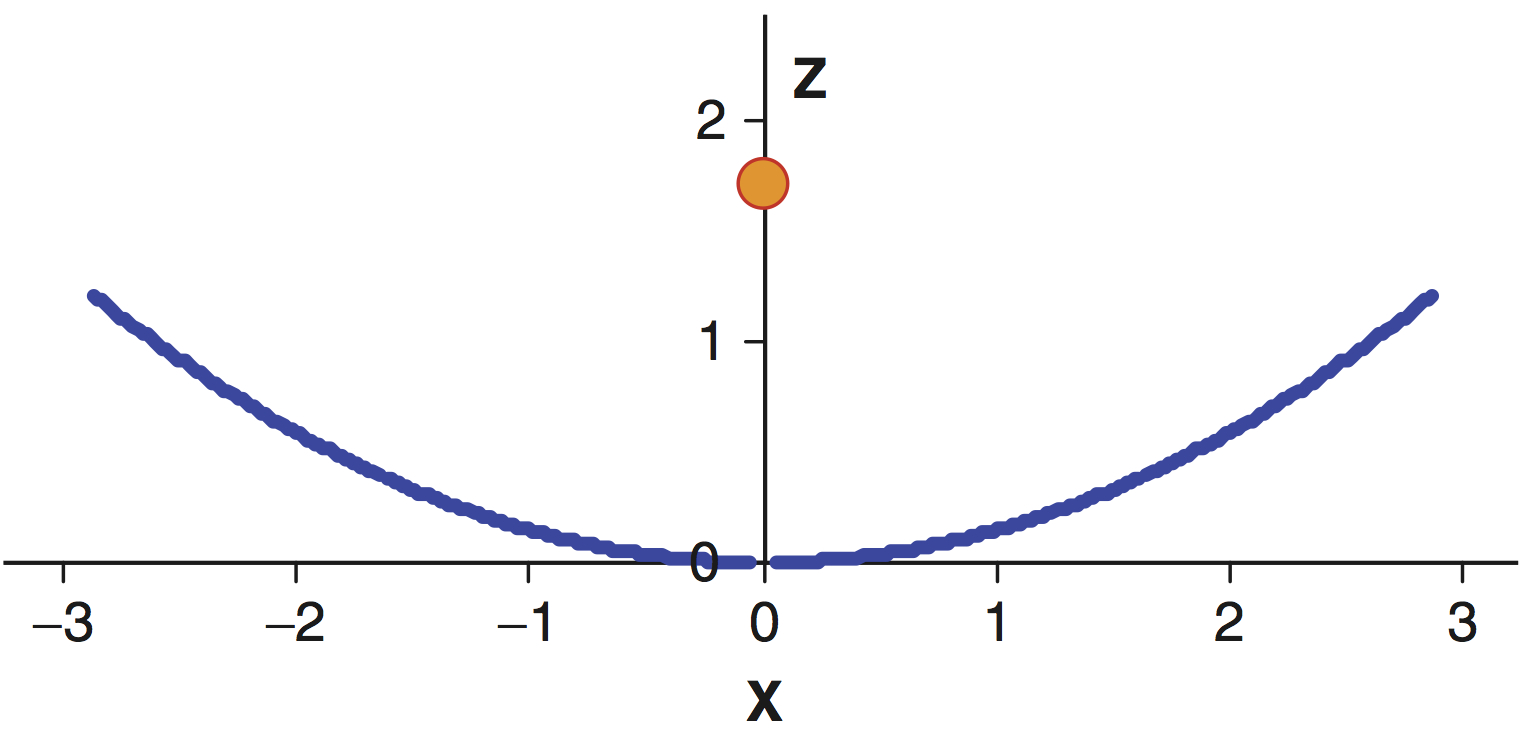
\includegraphics[width=0.6\linewidth]{FIG/PTC_section}
\caption[PTC section – dimensions of EuroTrough, LS-3, and other designs, in meters.]{PTC section – dimensions of EuroTrough, LS-3, and other designs, in meters \cite{Lupfert2013}.}\label{PTC_section}
\end{figure}
\\
The history of PTC goes far back to 1870, where they already used small engines with solar power \cite{Fernandez-Garcia2010}. With the time of the first oil crisis in the 1980s also new PTC were developed. In this decade also the collector family LS-1, LS-2 and LS-3 was developed by LUZ. These PCT  were implement in the first large-scale solar thermal power plants SEGS 1 (1984) to SEGS 9 (1990) in California. The used PTC features a modular design based on steel structures with parabolic preshaped, silvered glass mirrors and improved efficiency by implementation of evacuated tube receivers. A European consortium designed in the late 1990s the EuroTrough. Which was based on the LS-3 concentrator geometry with a focal length (the shortest distance from the mirror to the focal line) of 1.71~m and an aperture (the projection of the concentrator area in the direction of the optical axis) width of 5.77~m, but offered advantages in stiffness and costs \cite{Osuna2001}. Some years later, SENER developed a different structural approach, but still maintained the basics of LS-3 concentrator geometry \cite{Fernandez-Garcia2010}.
\begin{figure}[!h] 
\centering
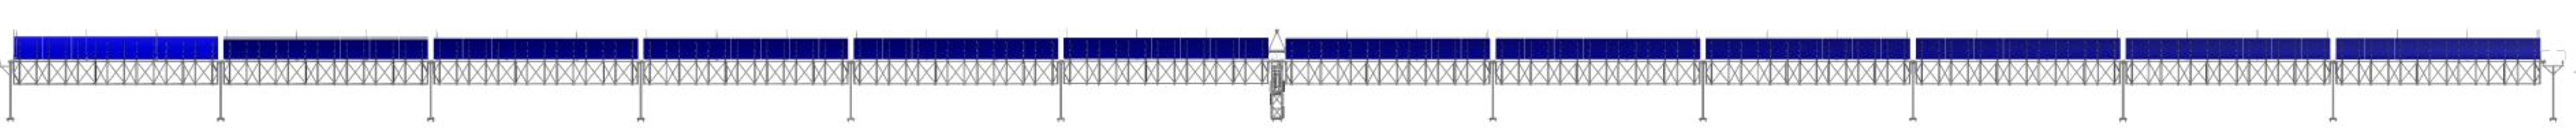
\includegraphics[width=1\linewidth]{FIG/SCA_EuroTrough}
\caption[Solar Collector Assembly (SCA) composed of 12 EuroTrough collector elements (SCE).]{Solar Collector Assembly (SCA) composed of 12 EuroTrough collector elements (SCE) \cite{VonReeken2014}.}\label{SCA_EuroTrough}
\end{figure}
\\
PTC are typically assembled from solar collector element (SCE), mounted on a series of aligned pylons. The center pylon is equipped with a hydraulic drive system to allow tracking of the total solar collector assembly (SCA). Figure~\ref{SCA_EuroTrough} shows the SCA of the EuroTrough. From 12 SCE of the SCA results a total length of approximately 150~m and 816~m$^2$ \cite{VonReeken2014}. \\
Table \ref{tbl: TroughCharacteristics} illustrates that recent developments show a continuing trend towards larger aperture sizes such as for the Heliotrough, Senertrough-2 and Ultimate Trough. The development steps of the aperture size are exemplary shown in Figure \ref{Kollektoren} for EuroTrough, Heliotrough and Ultimate-Trough. \\
\begin{table}[h!]  
  \centering
	\begin{tabular}{  p{3.3cm}  C{1.0cm}  C{1.0cm}  C{1.5cm}  C{1.0cm}  C{1.0cm}  C{1.0cm}  C{1.0cm}  C{1.5cm}} 
\hline
\textbf{Property} & \textbf{LS-1} & \textbf{LS-2} & \textbf{LS-3} & \textbf{Euro-Trough} & \textbf{Helio-trough} & \textbf{Sener-trough-1} & \textbf{Sener-trough-2} & \textbf{Ultimate-Trough} \\ \hline \hline
Start of development & 1984 & 1985 & 1989 & 1998 & 2005 & 2005 & 2006 & 2009 \\ \hline
Aperture width [m] & 2.55 & 5.00 & 5.77 & 5.77 & 6.78 & 5.77 & 6.87 & 7.51 \\ \hline
Length per module/SCE [m] & 6.3 & 8 & 12 & 12 & 19 & 12.27 & 13.23 & 24 \\ \hline
SCA length [m] & 50.2 & 47.1 & 99 & 147.8 & 191 & n.a. & 158.8 & 242.2 \\ \hline
Focal length [m] & 0.68 & 1.40 & 1.71 & 1.71 & 1.71 & 1.71 & 2 & n.a. \\ \hline
\end{tabular}
\caption[Characteristics of different parabolic trough collectors.]{Characteristics of different parabolic trough collectors \cite{Pitz-Paal.2013}.}\label{tbl: TroughCharacteristics}
\end{table}
\\
The use of lager collector units with more aperture area brings some advantages. The Ultimate Trough shows a cost reduction of about 20 to 25\% compared to the EuroTrough. Coming from lower specific costs and increased of optical performance. Also the amount of heat transfer fluid can be reduced by 25\%. This promise an decreased LCoE by about 11\% compared to EuroTrough. \cite{VonReeken2014}
\begin{figure}[!h] 
\centering
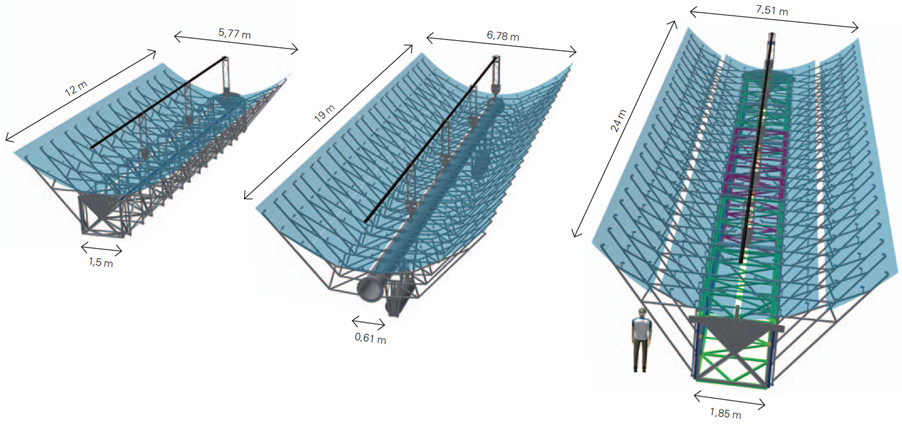
\includegraphics[width=1\linewidth]{FIG/Kollektoren}
\caption[Evolution of parabolic trough collector sizes over 3 development cycles (Eurotrough, HelioTrough, Ultimate Trough).]{Evolution of parabolic trough collector sizes over 3 development cycles (Eurotrough, HelioTrough, Ultimate Trough)\cite{Schlaichbergermannundpartner}.}\label{Kollektoren}
\end{figure}
\\
Another approach to reduce costs is the utilization of other reflector materials. The Skytrough uses reflectors made from silvered polymer film laminated to aluminum sheets mounted on a space frame. Compared the to the costs of components of the EuroTrough, the Skytrough contribute an additional 34\% cost savings in combination with a aperture width of 6.0~m \cite{Mason2014}. Thin glass on a glass-fiber/foam sandwich was used for the SL4600 construction \cite{SolarliteCSPTechnologyGmbH2014}. Both approaches take advantage of the mechanical strength of the mirrors to reduce the amount of additional steel structure required.\\
Abengoa Solar is developing currently the "SpaceTube" concept, using 8~m aperture width and will use 80~mm diameter absorber tubes. \cite{Olar2013}
\pagebreak
\subsubsection{Absorber tube (Receiver)}
The absorber tube or also called receiver is the component where solar energy is converted to thermal energy in the form of sensible or latent heat of the fluid that circulates through it. This component produces the predominant share of thermal losses in an parabolic trough power plant, for that reason it is also one of the most critical and important performance components \cite{Lupfert2013}. Currently, there are just two types of receiver for parabolic trough power plants, classified as either evacuated or non-evacuated. Evacuated receivers are commonly used for temperatures above 300$\,^{\circ}\mathrm{C}$ and its consist of three main parts. The metal absorber tube, an protection glass tube and the connection unit with expansion bellows. In order to reduce thermal losses and increasing the overall efficiency of the PTC the receiver unit uses a high vacuum (i.e.,~10-5~mbar) between the metal absorber tube and the protection glass. Figure shows \ref{absorber_tube} the structure of an typical vacuum tube receiver. 
\begin{figure}[!h] 
\centering
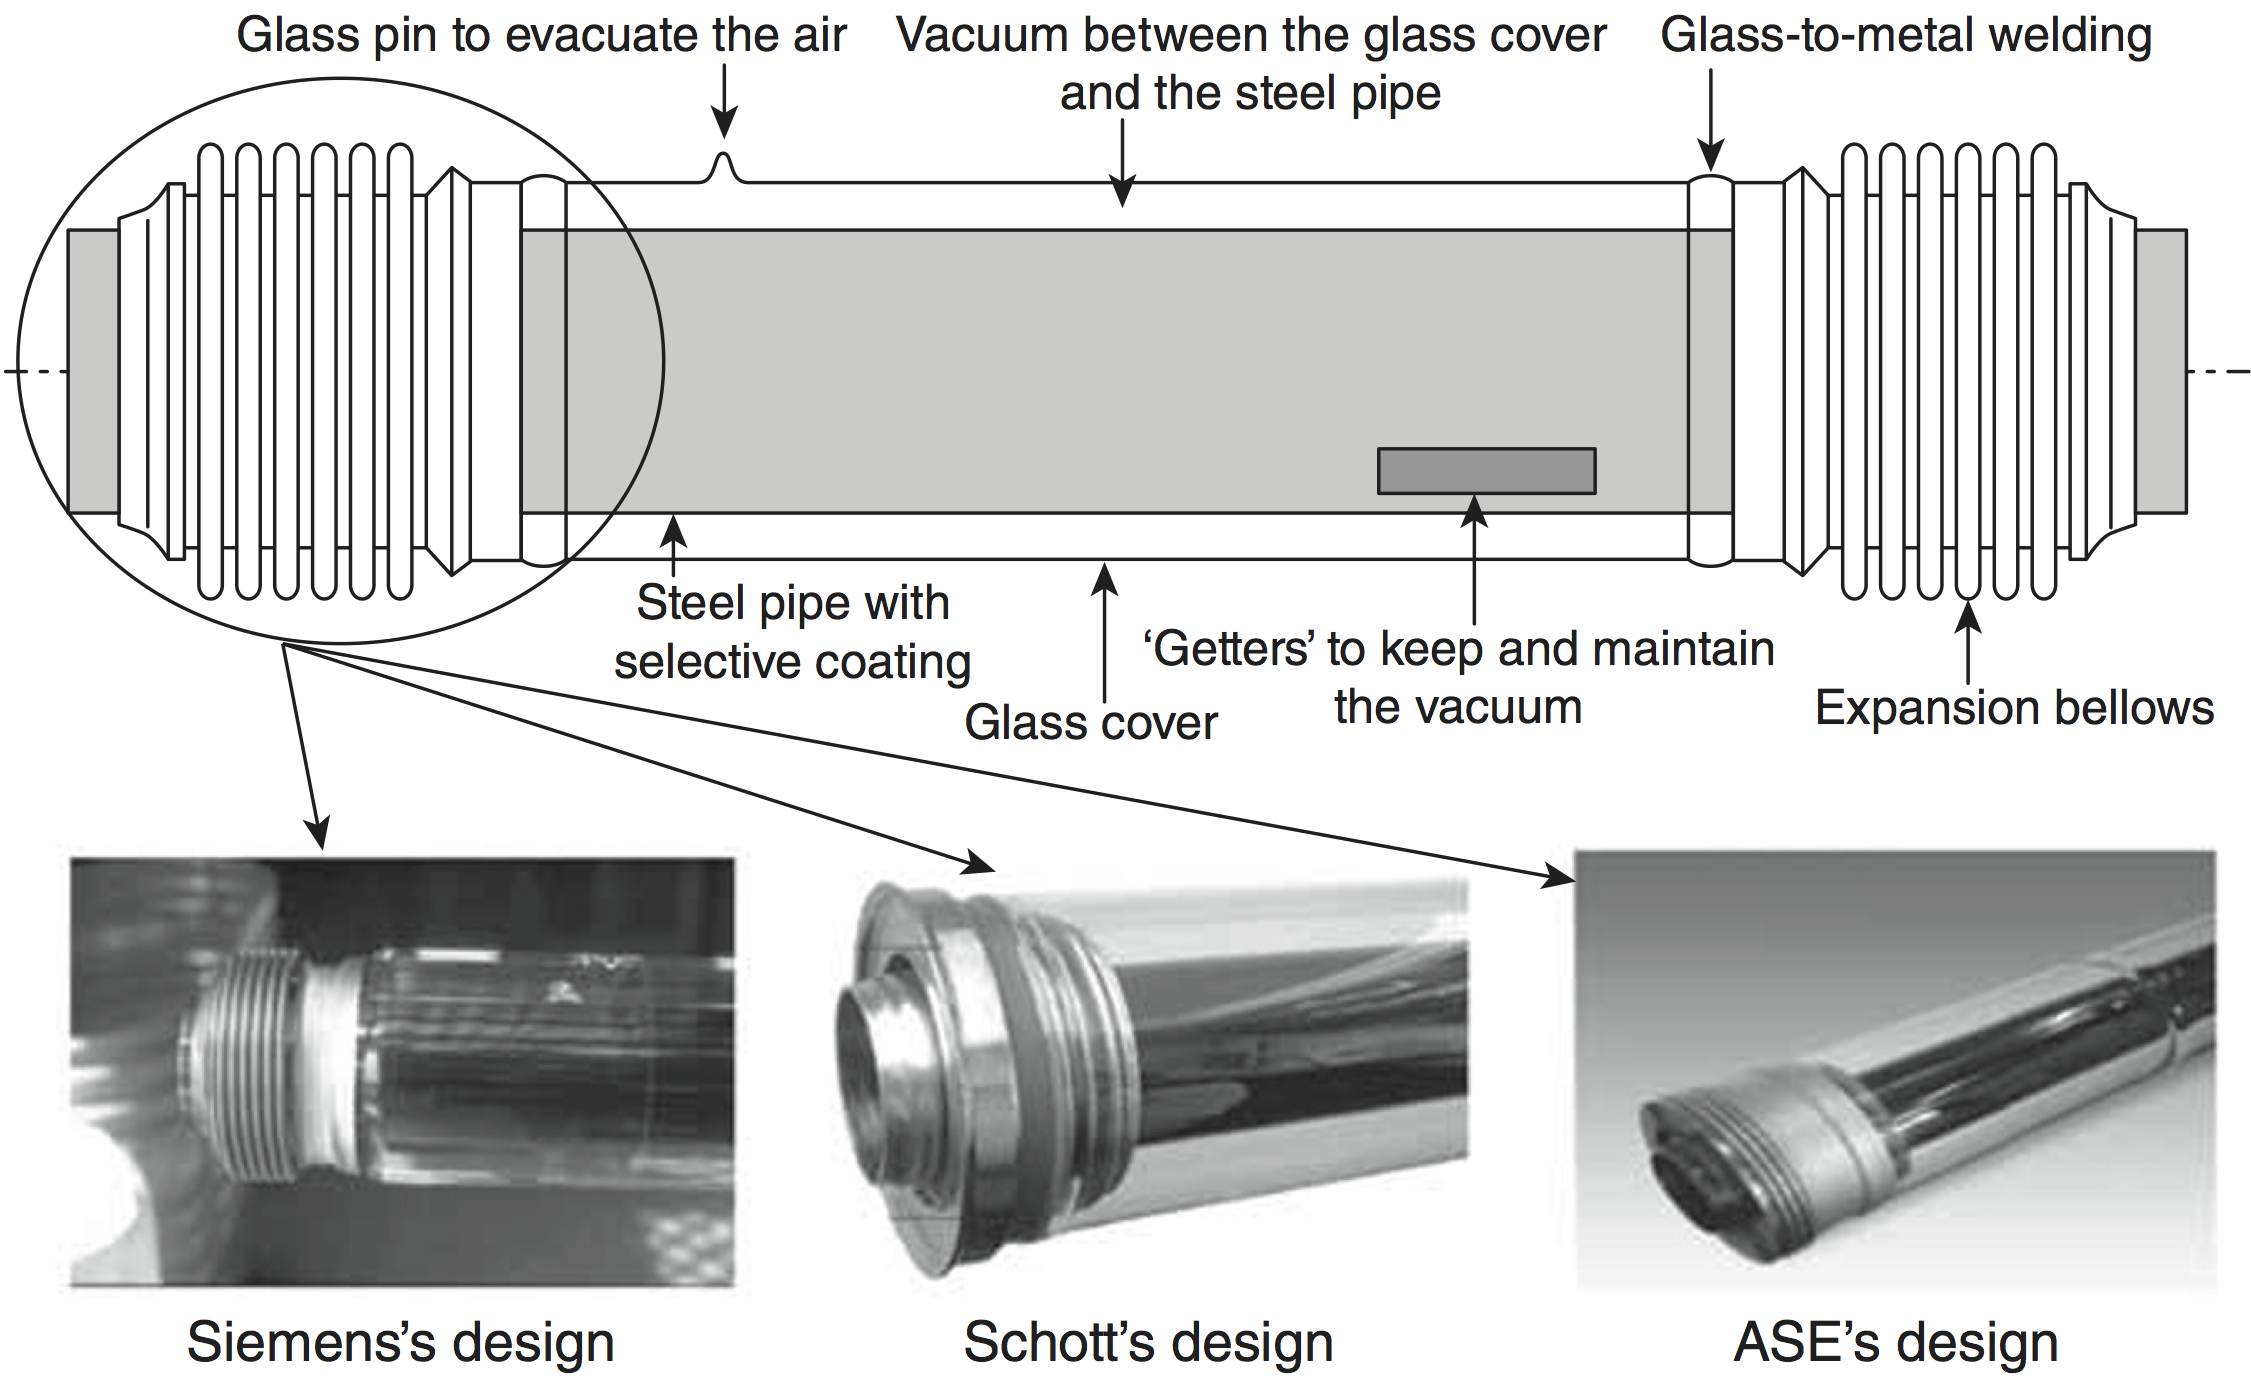
\includegraphics[width=0.9\linewidth]{FIG/absorber_tube}
\caption[A typical evacuated receiver for parabolic-trough collectors.]{A typical evacuated receiver for parabolic-trough collectors \cite{Moya2012}.}\label{absorber_tube}
\end{figure}
\\\\
The metal absorber tube is a dark-coated to absorb the incoming solar radiation. It absorbs the concentrated radiation reflected from the mirror, and also the global radiation hitting from top. The outer surface of the metal absorber tube has an optically selective surface with a high solar absorptance and low emittance for thermally generated infrared radiation. This is achieved with sputtered Cermet coatings consisting of several layers of metallic and ceramic coatings. Also, galvanic black-nickel and black-chrome coatings are applied but have less temperature resistance and higher emissivity. \cite{Platzer2012}\\
\\
The protection glass is connected to the metal absorber tube by means of stainless steel expansion bellows. These bellows compensate the thermal expansion of glass and steel which results at nominal working temperature. Therefore one end of these expansion bellows is directly welded to the outer surface of the metal absorber tube, while the other end is connected to the end of the protection glass by means of a glass-to-metal welding. The glass-to-metal welding is a weak point in the absorber system and has to be avoid by high thermal and mechanical stress that could cause the welding to crack. The receiver provider has various solution for the expansions bellows. Figure \ref{absorber_tube} shows also the solutions of three manufacturers (Schott, Siemens and ASE) joining the protection glass and the inner metal absorber tube. The expansion bellows also provide a tight annular gap between both tubes to make the vacuum. To support the shelf life of the vacum chemical ‘getters’ can be placed in the gap between the metal absorber tube and the protection glass to absorb gas molecules.
\begin{table}[!h]  
  \centering
	\begin{tabular}{  p{3.5cm}  C{3.5cm}  C{3.5cm}  C{3.5cm} } 
	
	\hline	
 & \textbf{Schott PTR-70} & \textbf{Siemens UVAC-2010} & \textbf{ASE HEMS08}\\ \hline \hline

Solar absorptance & $\ge$~0.95 & $\ge$~0.96 & $\ge$~0.95 \\ \hline
Solar transmittance & $\ge$~0.96 & $\ge$~0.96 & n.a. \\ \hline
Thermal emittance & $\le$~0.1 at 400$\,^{\circ}\mathrm{C}$  & $\le$~0.9 at 400$\,^{\circ}\mathrm{C}$& $\le$~0.1 at 400$\,^{\circ}\mathrm{C}$  $\le$~0.14 at 580$\,^{\circ}\mathrm{C}$\\ 
Steel pipe inner/ outer diameters & 70/65~mm stainless steel & 70/65~mm stainless steel & 70/65~mm stainless steel \\ \hline
Thermal losses & 250 W/m at 400$\,^{\circ}\mathrm{C}$ & n.a. & 230 W/m at 400$\,^{\circ}\mathrm{C}$ \\ \hline
Glass cover & Borosilicate & Borosilicate & Borosilicate\\ \hline
Active length ratio at 350$\,^{\circ}\mathrm{C}$ & >96\% & 96.4\% & n.a.\\ \hline
Maximum fluid temperature & 400$\,^{\circ}\mathrm{C}$ & 400$\,^{\circ}\mathrm{C}$ & 550$\,^{\circ}\mathrm{C}$\\ \hline
\end{tabular}
\caption[Technical parameters of the receivers commercialized by Schott, Siemens and ASE.]{Technical parameters of the receivers commercialized by Schott, Siemens and ASE \cite{Moya2012}.}\label{tbl: receiver_details}
\end{table}
\\\\
Most of the parabolic-trough solar thermal power plants implemented around the world until 2009 had receivers manufactured by either the Israeli company, Solel (purchased in 2009 by Siemens and 2013 from Abengoa \cite{Alcauza2013}), or the German company, Schott. In 2009, the Italian company, Archimede Solar Energy (ASE), announced that they were launching a new receiver tube called HEMS08, suitable for fluids up to 550$\,^{\circ}\mathrm{C}$. The first plant using HEMS08 receivers was the Archimede Plant, located in Syracuse (Italy) and ready to operate in 2010 using molten salt as HTF. Most widespread geometry is the receiver, with 70~mm absorber tube diameter, but due to larger aperature width of the trough reflectors, also the absorber tube diameter is raising. The technical details of the receivers manufactured 2012 by Schott, Siemens and ASE are shown in Table \ref{tbl: receiver_details}. Schott's PTR-70 is now in the 4. generation, the actual UVAC 70-7G is now in production by Rioglass a subsidiary from Abengoa Solar and ASE's present molten salt receiver tube is the HCEMS-11, but in generally the technical parameters are still up-to-date \cite{Schott2015,ArchimedeSolarEnergy2015,RioglassSolarInternational2014}.
\\\\
Most widespread geometry is the receiver, with 70~mm absorber tube diameter, but due to larger aperature width of the trough reflectors, also the absorber tube diameter is raising. This is a further contribution to using molten salt as future HTF in large-scale PTC power plants. 
\pagebreak
\subsubsection{Field}
The heat-collecting portion of the PTC power plant is the solar field. It consists of one or more parallel loops of SCAs. A common header pipe provides each loop with an equal flow rate of HTF. A second header collects the hot HTF to return it either directly to the power cycle for power generation or to the thermal energy storage system for use at a later time. To minimize pumping pressure losses, the field is typically divided into multiple sections, each section with its own header set, and the power cycle is situated near the middle of the field. The size of the field depends on required thermal power for the power block and the storage system. The orientation of the field depends obviously on the orientation of the parabolic collectors, which are installed with their north-south oriented rotation axis.
\begin{figure}[!h] 
\centering
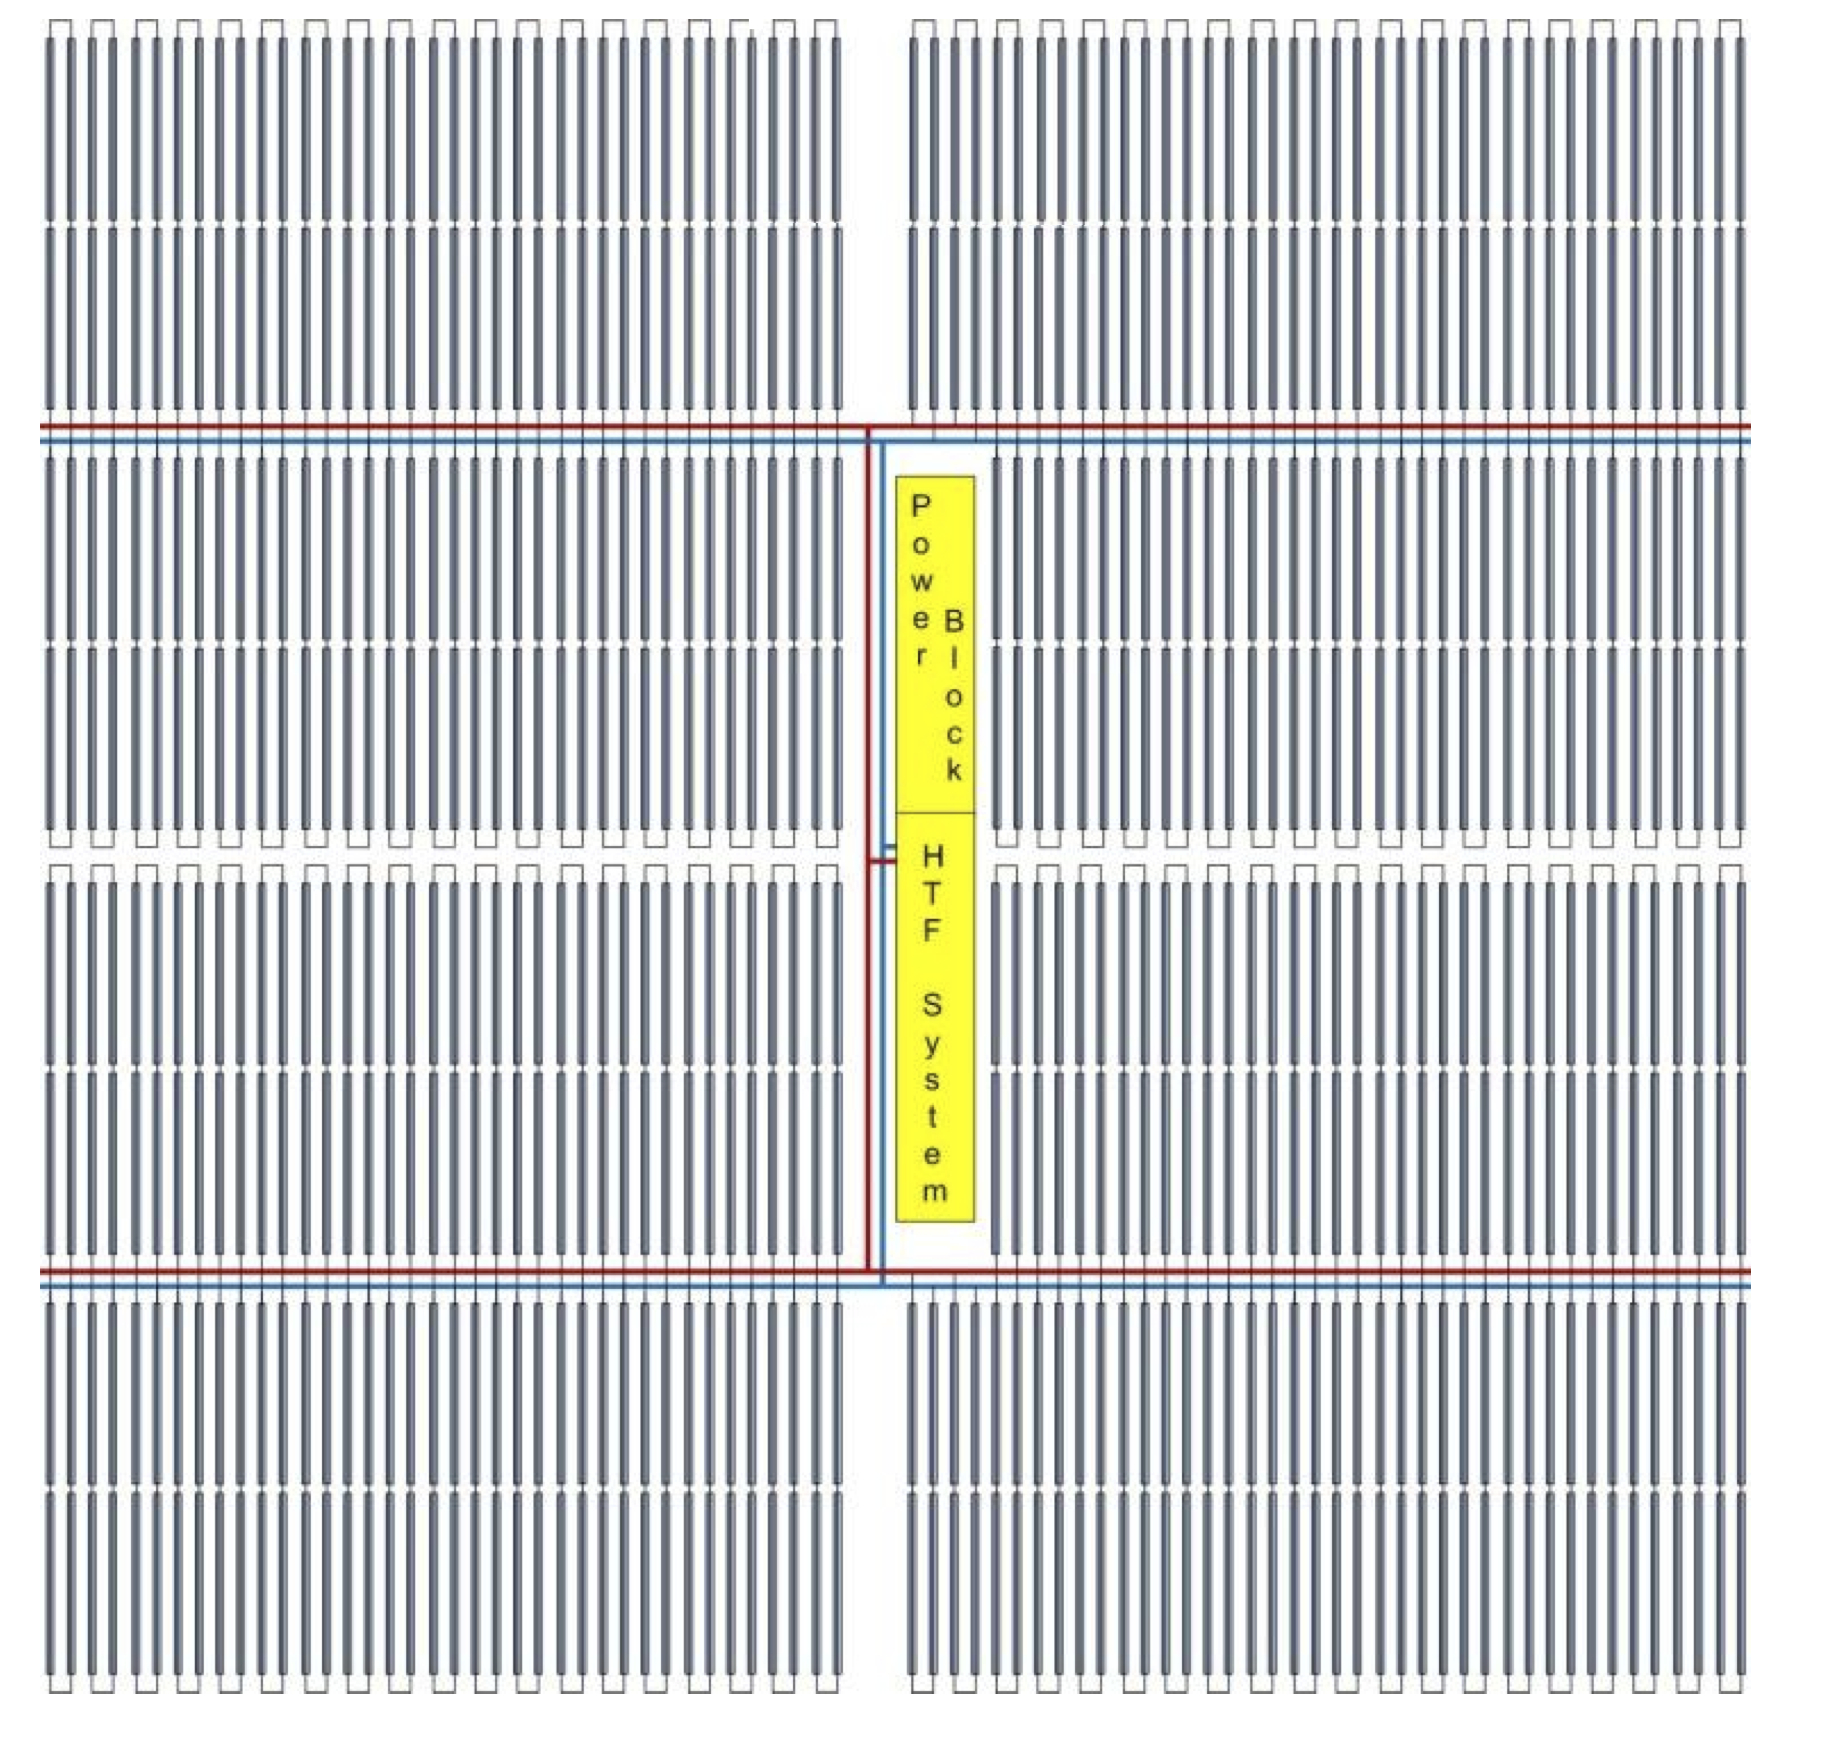
\includegraphics[width=0.7\linewidth]{FIG/PTC_field_EuroTrough}
\caption[Example of a EuroTrough collector field layout with 152 loops.]{Example of EuroTrough collector field layout with 152 loops \cite{VonReeken2014}.}\label{PTC_field_EuroTrough}
\end{figure}
Figure \ref{PTC_field_EuroTrough} shows one example plant layout for where  152 total loops are used, each loop with four SCA. The loop length depends on heat transfer fluid properties and rise in temperatures between inlet and outlet temperature ($\Delta T$). The flow rates through the receivers must be high enough to ensure appropriate heat removal from the absorber walls and low enough to keep pumping power for the fluid reasonably low.
\pagebreak
\subsubsection{Current stage of commercial scale PTC power plants}
On the commercial  scale the "Solana Generating Station" is currently one of the world largest PTC power plants. It was built from December 2010 to October 2013 southwest of Phoenix, Arizona. The solar-field aperture area of 2~200~000~m$^2$ concentrates in 808 loops with 4 SCA per loop drives two 140~MW$_{el}$ turbines. This plant uses synthetic oil as HTF and has a storage capacity of 6~h in molten salt (described in Chapter \ref{Subsection_storage_system}). The fed-in tariff of approx. 944~GWh/a is fixed for 30 years. The costs of the plant were approx. 2 USD billion. This power plant constitutes the current state of art in commercial scale PTC systems. \cite{NREL2015d}
\begin{figure}[!h] 
\centering
\includegraphics[width=1\linewidth]{FIG/PTC_Solana}
\caption[280-MW Solana PTC power plant near Phoenix, Arizona.]{280-MW Solana PTC power plant near Phoenix, Arizona \cite{AbengoaSolar2013a}.}\label{PTC_Solana}
\end{figure}
\pagebreak
\subsection{Central tower concentrating solar power} \label{subsection_CRS}
Central receiver systems (CRS) use a large number of reflectors (heliostats) to concentrate direct solar radiation to a focal point, in most cases on top of a tower. In order to reflect the incident sunlight to the focal point, the heliostats are tracked in two dimensions. The receiver is located at the focal point. The receiver absorbs the concentrated solar radiation and heats a HTF, such as a liquid or a gas. The generated heat drives a turbine to produce electricity by a generator. The basic principle of a solar CR power plant is shown schematically in Figure~\ref{power_tower}. Average concentration levels on the receiver are typically in the range 500-1~000 kW/m$^2$ \cite{Pitz-Paal.2013}. This concentration level is significantly higher than those achievable in linear focus systems such as PTC systems. The higher concentration level enables higher operational temperatures in the receiver, while maintaining good thermal efficiencies.
\begin{figure}[!h] 
\centering
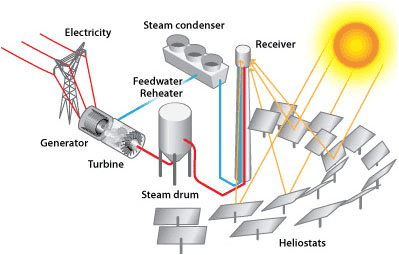
\includegraphics[width=0.6\linewidth]{FIG/power_tower}
\caption[Schematic CR power plant concept.]{Schematic CR power plant concept \cite{U.S.DOE2013}.}\label{power_tower}
\end{figure}
\\
A variety of solar tower concepts exist or are under development. These concepts differ mainly in the type of heat transfer medium, which dominates the layout and selection of all other components except for the heliostat field. Liquid or gaseous HTFs are state-of-the-art in solar tower technology. Water/steam, molten salt, and air are typical fluids \cite{Pitz-Paal.2013}. A HTF in a central receiver absorbs the highly concentrated radiation reflected by the heliostats and converts it into thermal energy to be used for the subsequent generation of superheated steam for turbine operation. The different HTF mediums are described in  chapter \ref{subsection_HTF}. Not like the more or less uniform design of PTC systems is the optical design and optimization of CRS more complicated. A multitude of variables one must be consider such as the continuous variation in configuration and performance of each of the heliostats as they track the sun and interact with one another. \\
The first documented concept of using ground-based segments (heliostats) to reflect direct-beam sunlight on a receiver comes from the Russian Victor Baum \cite{Baum1957}. But at this point no experimental device was built.\\
After several central receiver concepts and first 'commercial' used heliostats \cite{Trombe1957}, Alvin Hildebrandt published in 1972 the basic concept of nowadays CR systems as a hemispherical or cylindrical receiver atop a tall tower surrounded by a field of carefully positioned heliostats. The described power plant should have a tower height of 450~m with an heliostat field of 1.8~km diameter and produce 565~MW$_{th}$. There were no technical impediments expected with the tower or heliostat field. \cite{Hildebrandt1972}\\
Outgoing from more basic concepts and further research the Solar One, a 10~MW$_{el}$ CR ‘pilot plant’ was operated successfully from 1982 to 1988, in the desert near Barstow, California. This facility used a cylindrical receiver with water-steam as HTF at the focal point in 76~m height. The tower was surrounded by 1~818 heliostats, each with almost 40~m$^2$ area. After several problems in terms of storage and continuous turbine operation, the Solar One was upgraded to the Solar Two using molten salt as HTF and as direct storage concept. The Solar Two operated from 1996 to 1999 pumping molten nitrate salt at 290$\,^{\circ}\mathrm{C}$ from a cold storage tank through the receiver, where it was heated up to approximately 565$\,^{\circ}\mathrm{C}$ and afterwards to a storage tank, which had a storage capacity of 3~h. A simplified scheme of the Solar Two system is shown in Figure~\ref{towerdirecttwotank} on Page~\pageref{towerdirecttwotank}. \cite{Reilly2001}\\
The Planta Solar 10 (PS10) is the first solar central-receiver system producing grid-connected electricity under a purely commercial approach and started generating 11~MW$_{el}$ in 2007 near Seville, Spain. 624 heliostats with surface area of 120~m$^2$ each, concentrates direct irradiance to a cavity receiver using saturated steam as HTF on top of a 115~m high tower. The function of the PS10 is schematically shown in Figure~\ref{directsteamgeneration}.
\begin{figure}[!h] 
\centering
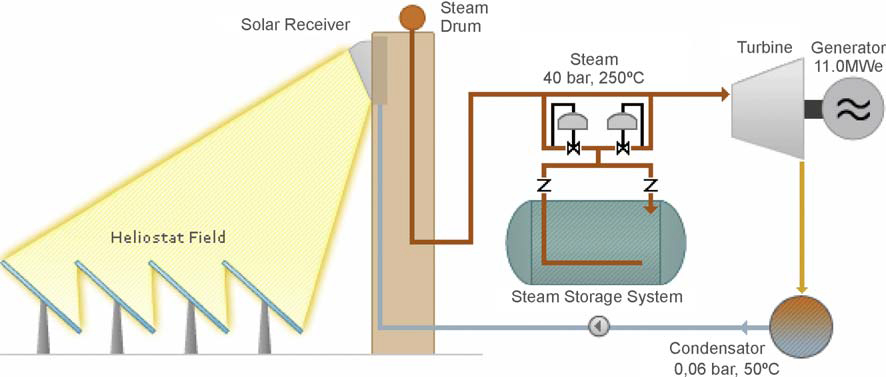
\includegraphics[width=0.7\linewidth]{FIG/directsteamgeneration}
\caption[Schematic diagram of the PS10 solar tower using water/steam as HTF.]{Schematic diagram of the PS10 solar tower using water/steam as HTF \cite{Medrano2010}.}\label{directsteamgeneration}
\end{figure}
\\
The first commercial solar thermal power plant to supply uninterrupted power for a full 24~h is the 19.9~MW$_{el}$ Gemasolar power plant, which started operation also near Seville in 2011. 2~650 heliostats focusing on the tube receiver on top of a 140~m height tower. The molten salt, which is used as HTF and for storage, reaching temperatures of 565$\,^{\circ}\mathrm{C}$.\\
Current commercial planned large-scale CR power plants are based on the PS10 and the Gemasolar power plant. Their main components are the heliostats and their field design, the receiver, and the tower itself. These are described bellow. Chapter \ref{Subsection_storage_system} examined the storage possibilities.  \pagebreak
\subsubsection{Heliostats}
Current heliostat technology differs mainly in the area of the reflecting surface. Studies of the heliostats area reaches from 1.1~m$^2$ up to 320~m$^2$ \cite{Tyner2014,Blackmon2012}. One of the largest heliostats in commercial application will have a total area of 140 m$^2$ \cite{Abengoa2014} and are built of several smaller facets, mounted on a back structure. Classical heliostat design is dominated by mirrors brought into position by steel structures and drives that guarantee high accuracies under wind loads and thermal stress situations. To the structures that hold the mirrors include struts, beams, the pylon, and the foundation. The linear actuators enable moving of the heliostat in two dimensions. There exists a zenith and an azimuth actuator together with their step motors. The orientation of the rotation axes may also differ between heliostat types. Several different types of heliostat mirrors exist. They can be differentiated according to size, shape, basic design concept, or even according to there tracking system. Each heliostat type has its own characteristics in terms of wind-performance and tracking during windy conditions, costs, and complexity of control. A field made up of more small heliostats will require a more complex control system than a field of fewer heliostats. Therby, large heliostats are mostly more cost-efficient than small ones (see Figure \ref{Heliostats}). Improvements in controllability may cause this to change, however, and several companies are attempting the strategy of many small heliostats as opposed to fewer large heliostats.
\begin{figure}[!h] 
\centering
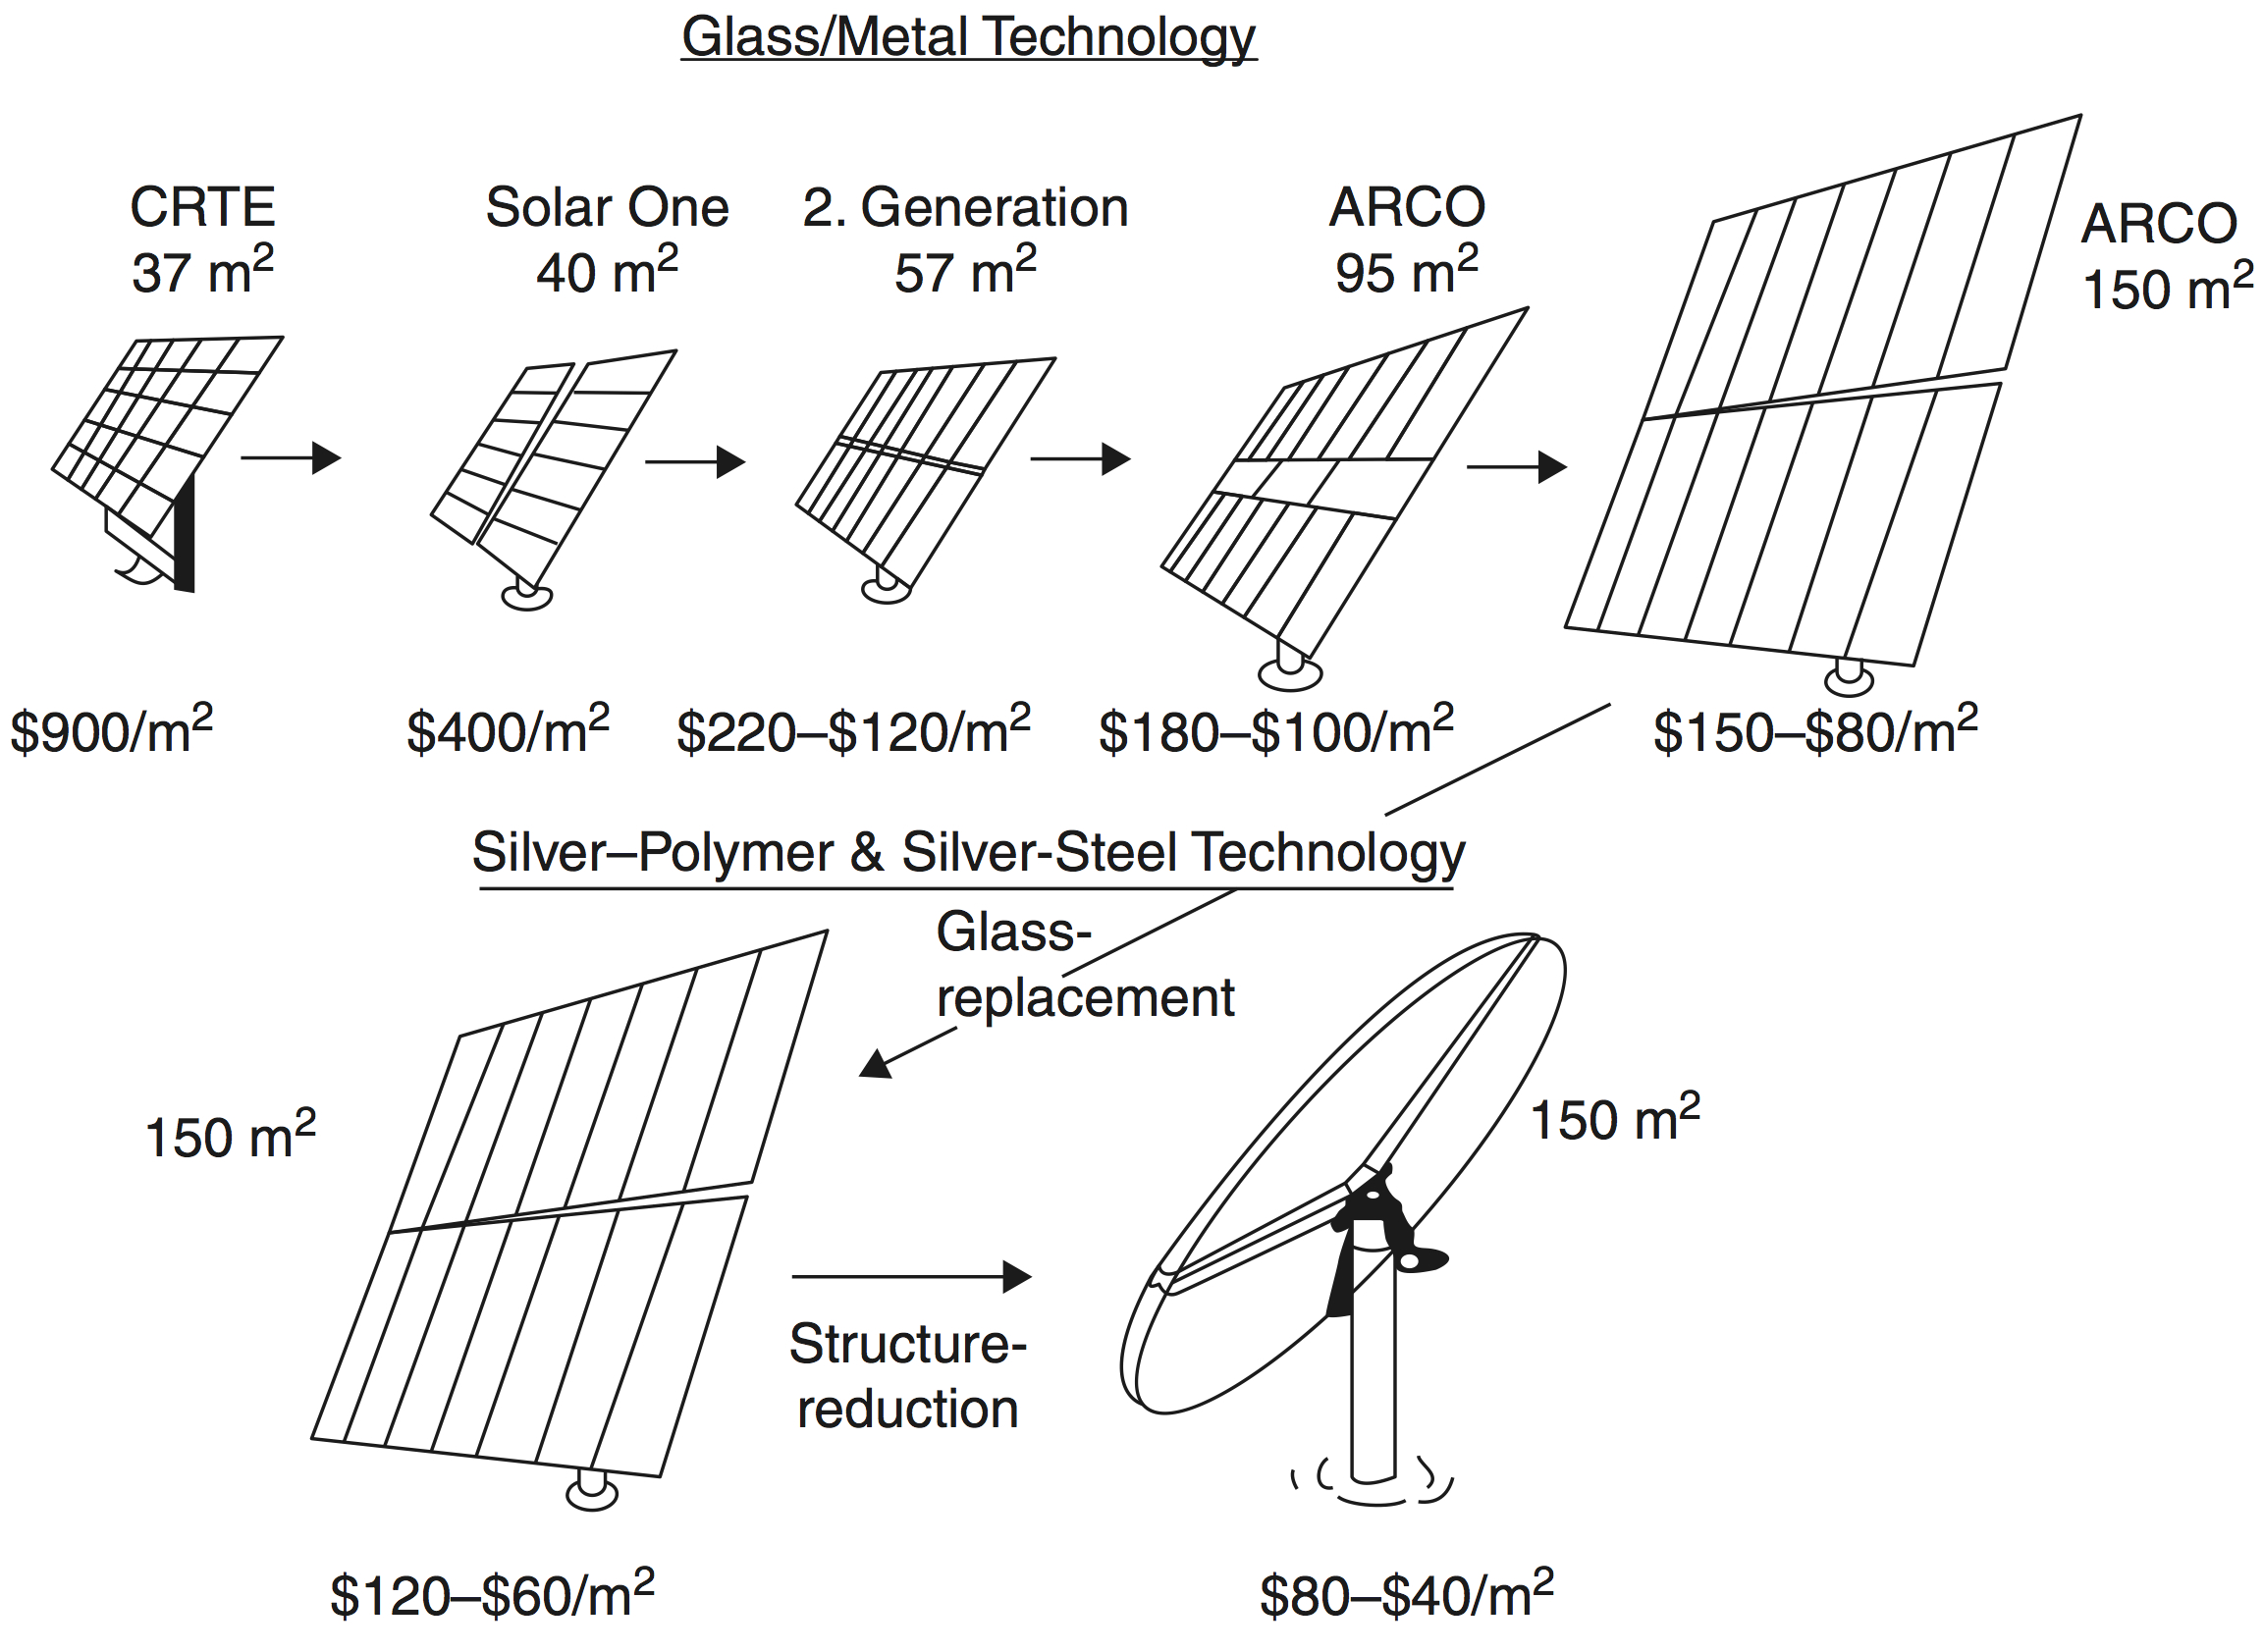
\includegraphics[width=0.9\linewidth]{FIG/Heliostats}
\caption[Heliostats used in solar power plants and their costs.]{Heliostats used in solar power plants and their costs \cite{Kolb2007}.}\label{Heliostats}
\end{figure}
\subsubsection{Heliostat field design}
The heliostat field layout is a complex topic. Decisions regarding the best position for locating heliostats relative to the receiver and how high to place the receiver above the field constitute a multifaceted problem, in which costs and heliostat loss mechanisms are among the variables, and which is solved by an iterative process. Therefore the location and the receiver type is decisive. In the northern hemisphere, the position of the sun is to the south of the plant and the field must be placed to the north of the tower. In the southern hemisphere the opposite is true. The general terminology for this position would be the "polar side" of the tower, which can be applied to towers in both the northern and southern hemispheres. The opposite side of the tower is the
"equatorial side" \cite{Alexopoulos2013}. The basically distinguishable field design types are shown in Figure \ref{Fielddesign} and can either surround the tower (Surround-field) for larger systems or be spread out on the shadow side of the tower (Polar-field) in the case of smaller systems.
\begin{figure}[!htbp]
        \centering
        \begin{subfigure}[b]{0.5\textwidth}
                \centering
                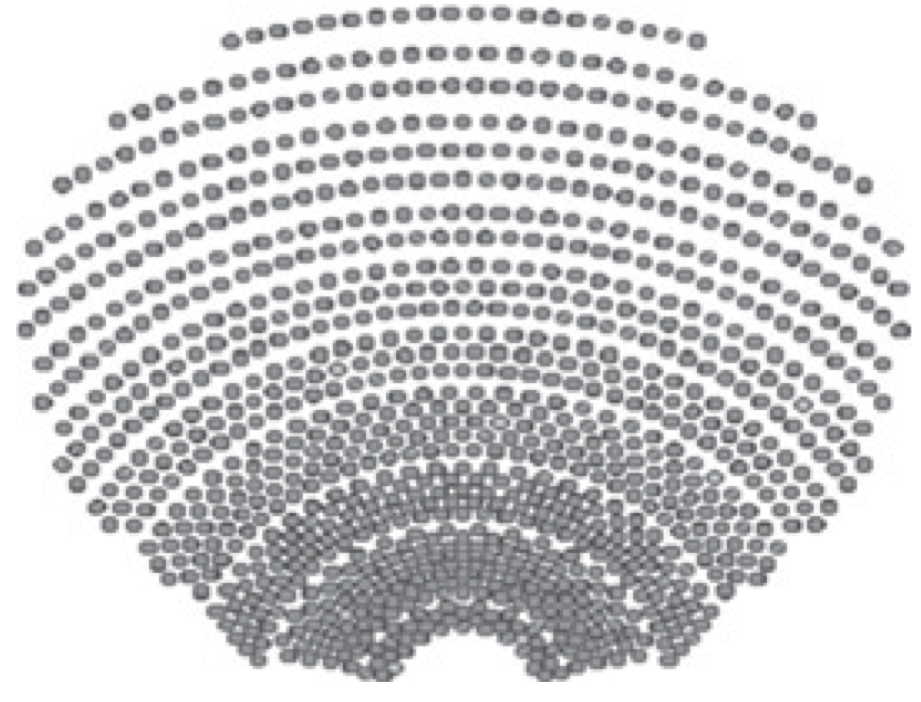
\includegraphics[width=0.9\textwidth]{FIG/north_field_layout}
                \caption{Polar-field layout.}\label{north_field_layout}
        \end{subfigure}%
        ~
        \begin{subfigure}[b]{0.5\textwidth}
                \centering
                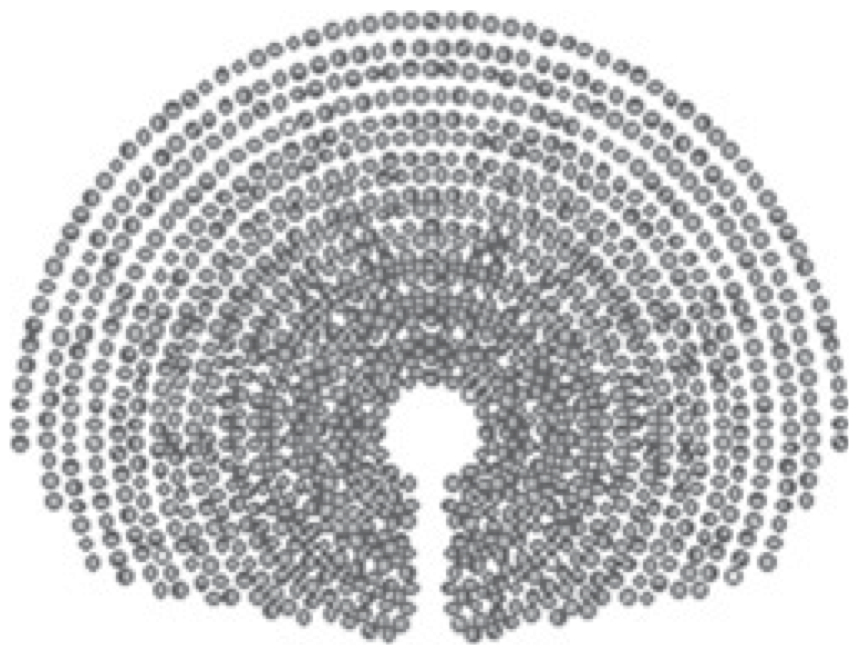
\includegraphics[width=0.9\textwidth]{FIG/sourround_field_layout}
                \caption{Surround-field layout.}\label{sourround_field_layout}
        \end{subfigure}
        \caption[Basically distinguishable field design types.]{Basically distinguishable field design types \cite{Kulichenko2012}.}\label{Fielddesign}
\end{figure}
With a field on only one side of the tower, a cavity receiver is usually used. Close to the equator, where the sun passes directly overhead, a surrounding-field can be used in combination with an open receiver (Tube receiver, see below). Another possibility is the use of two ore three fields – one on either side of the tower, in combination with a cavity receiver for each side (see Figure \ref{KhiSolarOneReceiver}). With higher power levels, surround field layouts are usually more economical. The higher the site latitude of a plant (i.e., the further away from the equator), the more the heliostat field tends to be shifted polewards. When laying out a heliostat field there are several types of losses that must be considered. These are not only the optical losses, so called, the cosine losses and losses due to shadowing, blocking, spillage (reflected radiation miss the receiver surface), and atmospheric attenuation, but also technical considerations, that is, the mirror reflectivity, mirror surface defects, tracking accuracy, wind load, and tower oscillations (due to wind load) as well as the heliostat fault rate. The aim in the designing of a heliostat field is to reliably produce the power required by the power block whilst keeping land usage and total costs to a minimum. \cite{Vant-Hull2012} \pagebreak
\subsubsection{Tower and receiver}
The function of the tower is to positioning the receiver in the required height above the heliostat field. So the choice of tower constructions depends primarily on the required height of the tower. But the height of the tower is limited by its cost. Towers are mainly constructed of steel or reinforced concrete. \\
\\
The function of a receiver is to absorb the concentrated solar irradiation energy impinging from the heliostat field and transfer it to the working fluid. Requirements to a solar receiver include high thermal conductivity, dark color of the body for high absorptivity, and temperature resistance. According to Prof. Dr. Hoffschmidt \cite{Hoffschmidt2014} from the German aerospace center (DLR) there are actually two main receiver types state of art for CR power plants, which uses molten salt and water for direct steam generation: external (tube) receiver and cavity receiver. 
\begin{figure}[!htbp]
        \centering
        \begin{subfigure}[b]{0.5\textwidth}
                \centering
                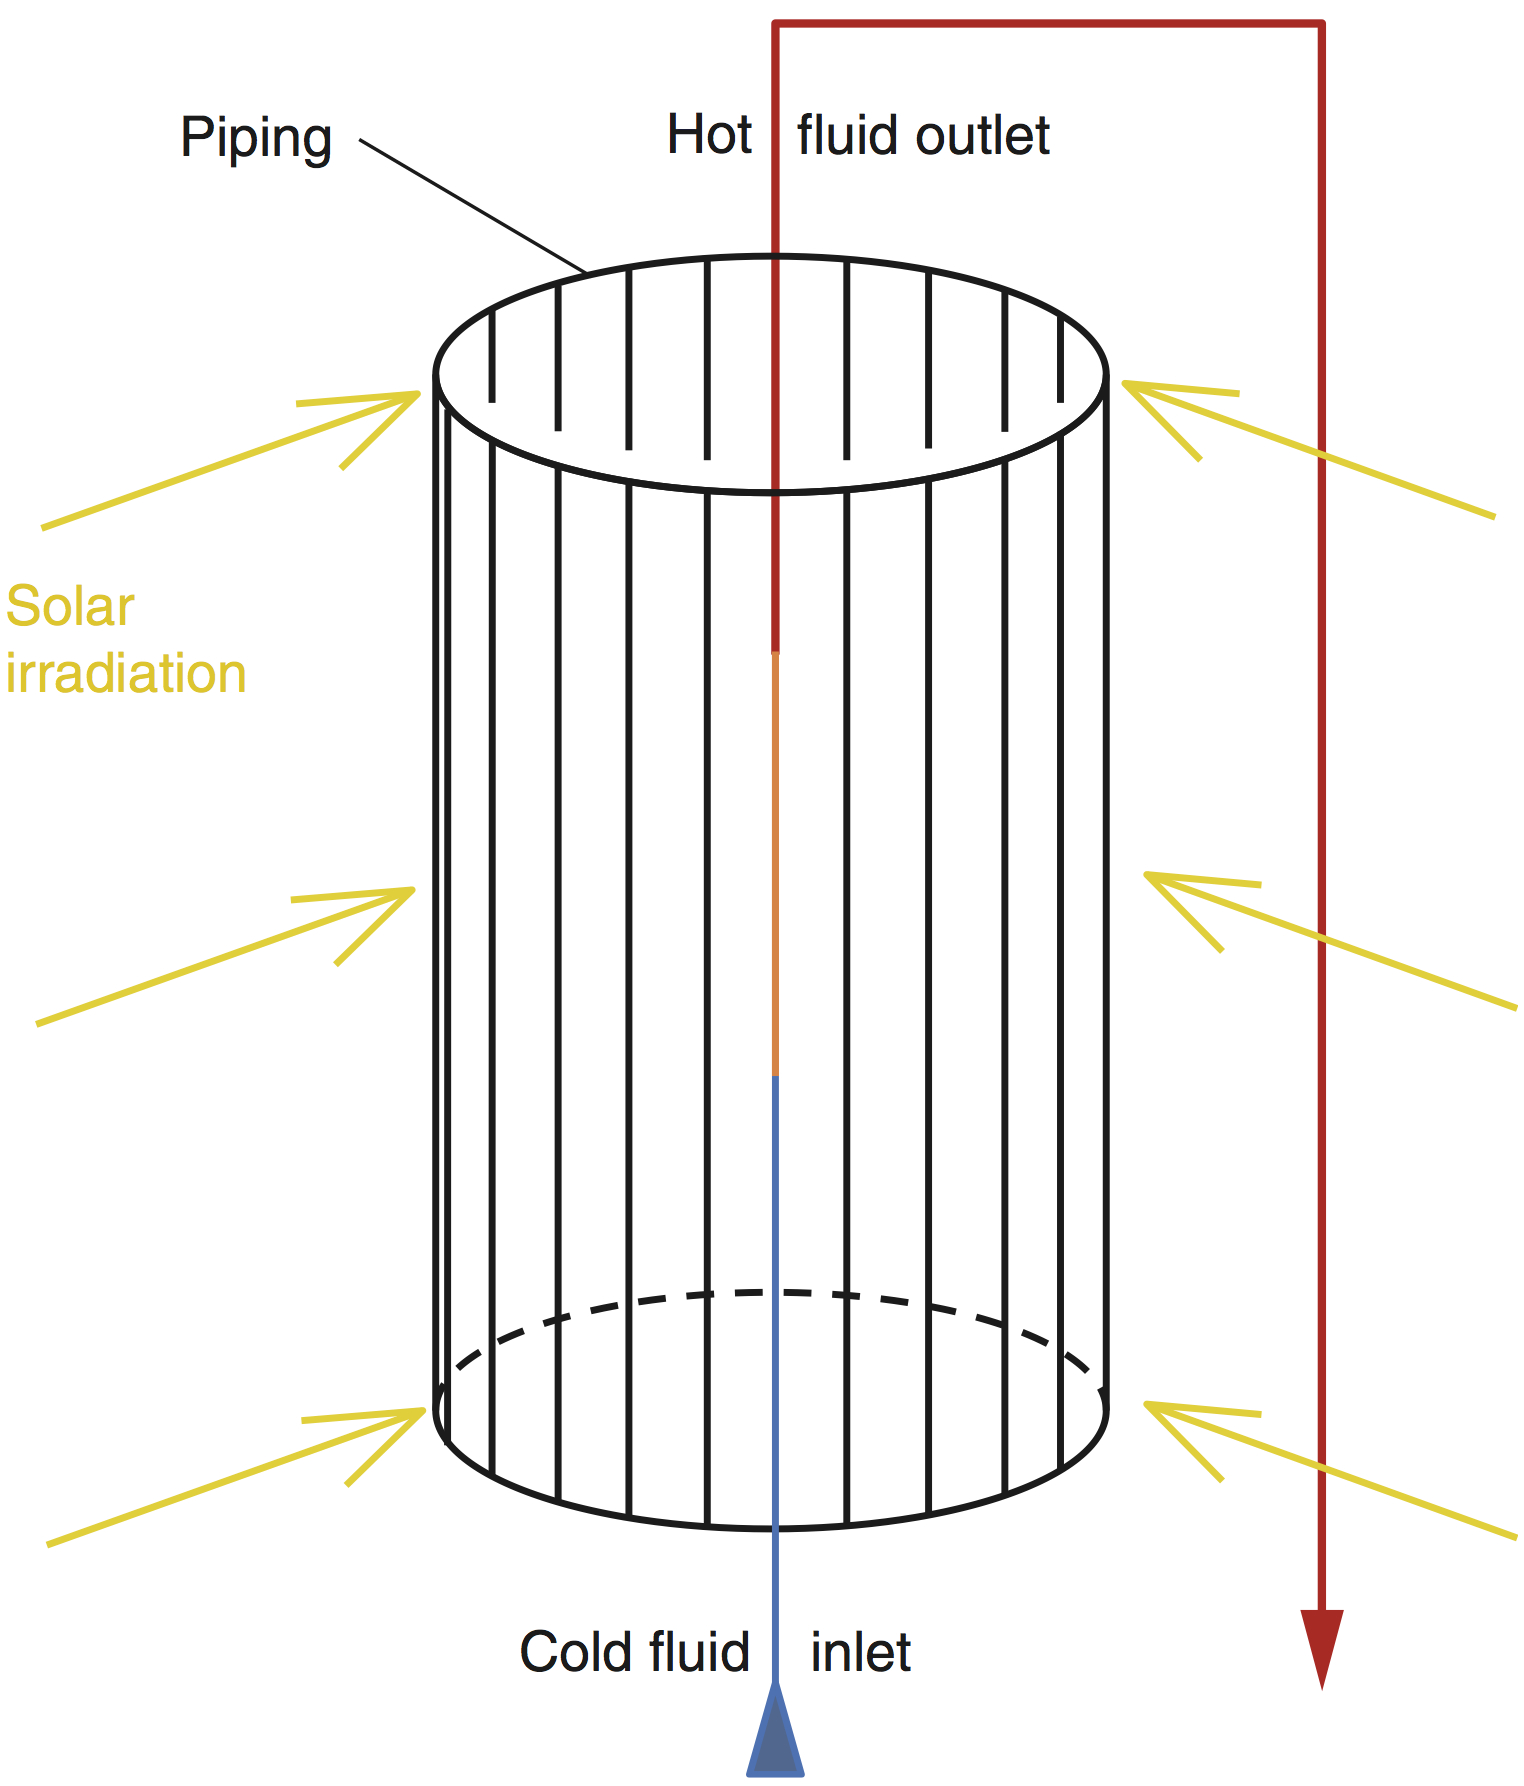
\includegraphics[width=0.9\textwidth]{FIG/TubeReceiver}
                \caption{External tube receiver concept \cite{Alexopoulos2013}.}\label{TubeReceiver}
        \end{subfigure}%
        ~
        \begin{subfigure}[b]{0.5\textwidth}
                \centering
                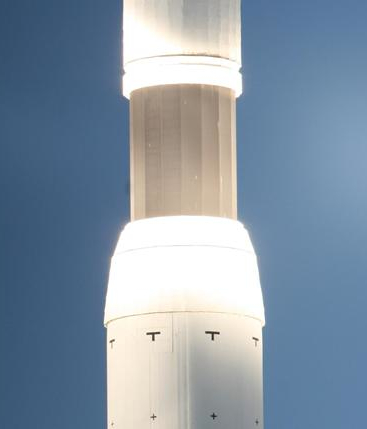
\includegraphics[width=0.9\textwidth]{FIG/Gemasolar_tower_heatshield}
                \caption{External tube receiver implemented in Gemasolar power plant \cite{Microtherm2012}.}\label{Gemasolar_tower_heatshield}
        \end{subfigure}
        \caption[External tube receiver concept and example of application.]{External tube receiver concept and example of application.}\label{TubeReceiverConceptGemasolar}
\end{figure}
\\
An external receiver consists a large number of vertically arranged pipes or flat plates through which the HTF is pumped in upward direction. There are variations of shapes for the external receiver, mostly cylindrical or square-shaped. The tubes in the receiver can be crosswise arranged with different zones for pre-heating, evaporation and superheating (in case of super heated steam). Typical solar heat fluxes in this type of receiver are up to 1 MW/m$^2$ \cite{Pitz-Paal.2013}. An basic concept for an external receiver is shown in Figure \ref{TubeReceiver} with a cylindrical shape. An example for such a external tube receiver is the receiver of the Gemasolar power plant, that used molten salt as HTF. The receiver consists of a great number of HTF pipes. The external receiver pipes are fixed vertically whereby the salt smelt is pumped in upward direction. The receiver outlet temperature of the molten salt is approximately 565$\,^{\circ}\mathrm{C}$. The tube receiver of the Gemasolar power plant is shown in Figure \ref{Gemasolar_tower_heatshield}. An other example  is the Ivanpah Solar Electric Generating System (ISEGS) in California’s Mojave Desert where they produce direct steam at 550$\,^{\circ}\mathrm{C}$ using an external tube receiver which is square-shaped. A disadvantage for using the pipe receiver is the high reflection loss which is higher than for other receiver types. One way to reach reduction of thermal losses is an cavity arrangement and a face down arrangement. \cite{Hoffschmidt2014}
\begin{figure}[!htbp]
        \centering
        \begin{subfigure}[b]{0.5\textwidth}
                \centering
                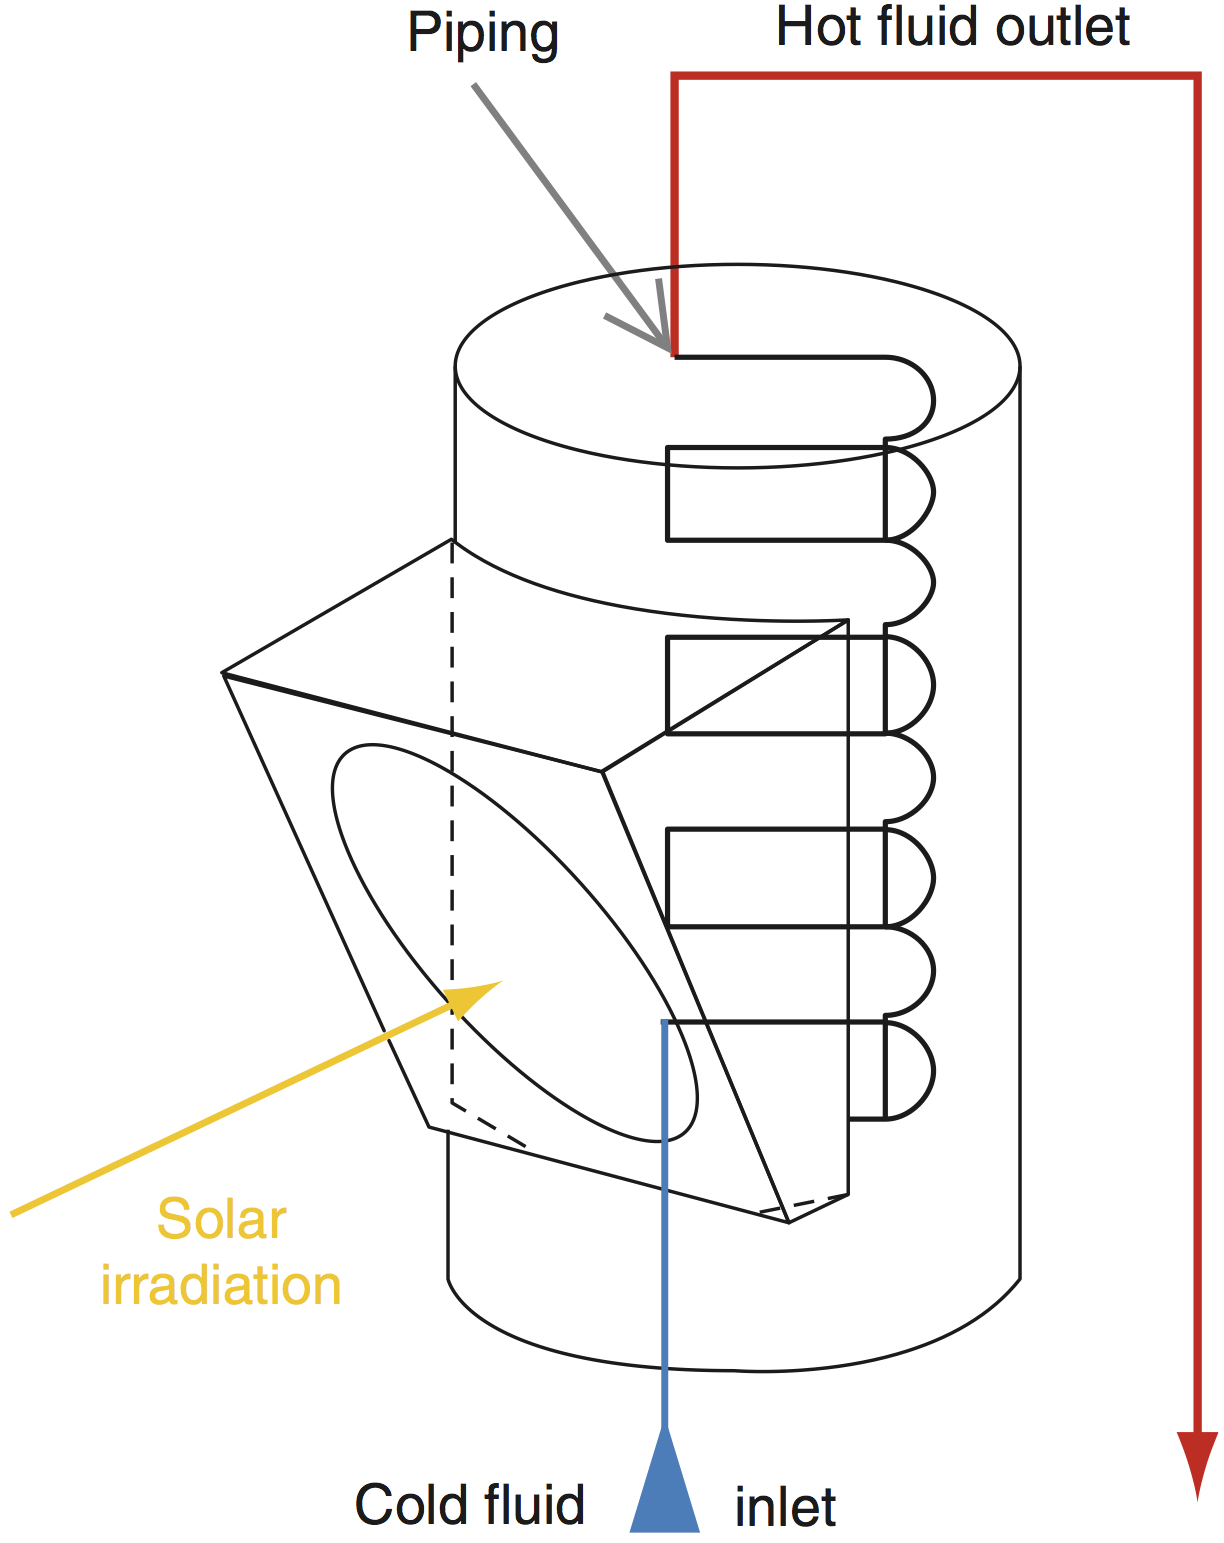
\includegraphics[width=0.9\textwidth]{FIG/CavityReceiver}
                \caption{Basic cavity receiver concept \cite{Alexopoulos2013}.}\label{CavityReceiver}
        \end{subfigure}%
        ~
        \begin{subfigure}[b]{0.5\textwidth}
                \centering
                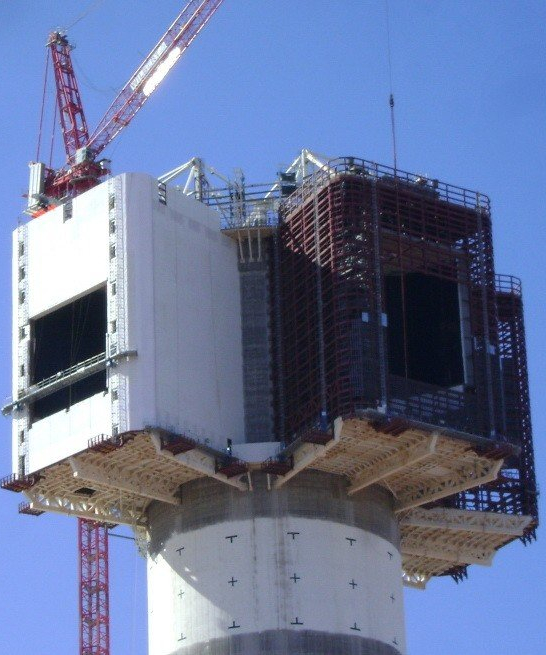
\includegraphics[width=0.9\textwidth]{FIG/KhiSolarOneReceiver}
                \caption{Three under construction situated cavity receiver mounted at the  Khi Solar One Tower \cite{CMI_Energy2015}.}\label{KhiSolarOneReceiver}
        \end{subfigure}
        \caption[Cacity receiver concept and example of application.]{Cavity receiver concept and example of application.}\label{CavityReceiverConceptKhiSolar}
\end{figure}
\\
A cavity receiver consists of a cavity with a small opening where the receiver is located. The concentrated solar irradiation is directed into the small opening where it impinges on tubes carrying the working fluid. The idea of the cavity receiver is the reduction of thermal and optical losses. From the radiation entering the inlet aperture, only small amounts are reflected back into the atmosphere through the inlet aperture. Figure \ref{CavityReceiver} shows the basic concept of an cavity receiver. The cavity receiver concept is implemented in the PS10 solar tower plant in Spain. The direct irradiated absorber tubes is basically a forced circulation radiant boiler with low ratio of steam at the panels output, which produce saturated steam at 250$\,^{\circ}\mathrm{C}$ and 40~bar. A schematic diagram of the PS10 is shown in Figure \ref{directsteamgeneration}. SA first solar power tower will also use a cavity receiver technology. Figure \ref{KhiSolarOneReceiver} shows the three under construction situated cavity receiver of the Khi Solar One. Two steam generator (east and west orientated) and one super heater (south orientated) using the cavity receiver concept are external mounted on the tower \cite{Prof.Dinter2015}.
\subsubsection{Current stage of commercial scale CR power plants}
As shown above there is a variety of CR concepts also for commercial scale. But there are three outstanding CR projects worth mentioning for large-scale commercial application. The Khi Solar One, the Ivanpah Solar Electric Generating System (ISEGS) and the Atacama-1.\\
\\
Fore SA obviously the Khi Solar One, which will be the first commercial scale CR power plant in the country. This 50.0~MW$_{el}$ power tower is under construction and will be operated by Abengoa Solar. The Polar-field consists out of 4~120 heliostats with a reflection surface of 140.0~m$^2$ each concentrate direct solar irradiance on three cavity receiver. \cite{NREL2014,Prof.Dinter2015}\\
\\
The Ivanpah Solar Electric Generating System (ISEGS) is currently the largest CSP plant operating by BrightSource. The three-unit power system with in total 377.0~MW was started operation 2014 in Ivanpah Dry Lake, California. The three external square-shaped receiver on each tower are focused by 173~500 heliostats with a aperture area of 15.0~m$^2$ each. The costs for the power plant which consists out of three CRS are approx. 2~200~USD million. But instead of an storage system BrightSource using a natural gas fired backup for the ISEGS. \cite{BrightSourceEnergy2014,NREL2014a}\\
\\
One of the highly promising CR projects for large-scale commercial application is Abengoa Solars Atacama-1. The eponymous Atacama desert in Chile, where the plant is under construction, has the highest levels of solar radiation worldwide. The scheduled operation start of the plant is in 2018. 10~600~heliostats each 140~m$^2$ in aperture area will concentrate on a external cylindrical shaped receiver with 32~m in height and 19~m in diameter. The receiver will be positioned in a 243~m-tower to heat molten salt to drive a 110~MW$_{el}$ steam turbine and 17.5~h direct thermal storage. This will generate electricity 24~h per day, similar to the Gemasolar power plant, but more than five times that powerful. This project constitutes the current state of art in commercial scale CRS. \cite{NREL2015b,AbengoaSolar2015a,AbengoaSolar2015}
\pagebreak
\subsection{Heat transfer fluid} \label{subsection_HTF}
In each CSP family, various options exist for the heat transfer fluid, the storage technology, and the thermodynamic cycle. The heat transfer fluid (HTF) removes heat from the receiver and transfer it either to the storage system or to the final use. The correct choice of the fluid is determinant in order to reduce costs and increase the efficiency of the plant. The most important HTFs are:
\begin{itemize}
\item \textbf{Synthetic oils} They are used predominant in PTCs thanks to their low pumping losses, their adequate conductivity and the fact that they do not need very high pressures, around 16 bar. However, they face a temperature limit of 393$\,^{\circ}\mathrm{C}$, which limits the efficiency of the plant. In addition, they are toxic and flammable.
\item \textbf{Direct steam generation} If saturated or superheated steam is generated directly at the receiver two main advantages are found: first, no heat exchanger is required in order to generate steam from the HTF and second, the exergy loss that takes place at such heat exchanger is avoided. However, some issues are also found: high pressures are required, which makes it not suitable for PTC's due to leakages at the movable elements, different thermal regimes are found in the steam generation, which complicates transients and superheating, and no efficient method has been found for energy storage. This last point is a main issue, especially when the importance of dispatchability is considered.
\item \textbf{Molten salts} Molten salts are playing a great role in CSP for energy storage. The most commercial molten salts have a working temperature range from 290$\,^{\circ}\mathrm{C}$ to 565$\,^{\circ}\mathrm{C}$, and thus higher efficiencies are obtained at the power block (cf. Table \ref{TableSensbleHeatStorageMaterial}). However, they have the issue of solidifying at relative high temperatures. As a result, if the receiver cannot be evacuated when there is no impinging sun, which is the working mechanisms in central towers with molten salts, the fluid must be recirculated from the hot tank to the cold tank, increasing thermal energy losses. Evacuation of linear receivers seems more difficult than in central towers due to the fact that tubes are horizontal.
\item \textbf{Pressurized gasses} Gasses do not have any limit in temperature, neither by the upper nor by the bottom part. In addition, they are cheap, especially if the air is used as it is found in the atmosphere. However, pumping losses are much higher than in liquid HTFs due to the density difference. In order to overcome this issue, pressure must be increased, pumping power losses being inversely proportional to the squared power of the pressure. At current time no commercial power station uses pressurized gases, although they have been used in central tower (Solgate) and CCP research prototypes. Leakages of the gas found in the movable elements of PTCs due to the high pressures suggest the need of fixed receivers in order to use pressurized gasses.
\end{itemize}
\subsection{Storage systems for CSP}\label{Subsection_storage_system}
The storage systems plays the decisive role that makes solar thermal power stand out from other renewable energy technologies. By the integration of heat storage capacity, STP plants are actually the only operational renewable energy option on the market offering dispatchable electricity power generation in multi-MW range. With the thermal energy storage (TES) system a CSP power plant offers the advantage of an integrated solution, which does not impose additional requirement on the electrical grid. Figure~\ref{integratedstoragescheme} shows the general scheme to store thermal energy into a CSP plant. The storage unit is connected both to the solar receiver and the power block. During charging the heat (high enthalpy mass flow) from the solar receiver is transferred to the thermal cycle, while the storage unit is charged by excess thermal heat. During the discharge process, the working fluid of the power block is heated by the energy from the  storage systems. Alone or in combination with some fossil fuel backup, the storage system keeps the plant running under full-load conditions. The energy from the storage might be also used to preheat the collector system during the ramp up time of the power plant.
\begin{figure}[h] 
\centering
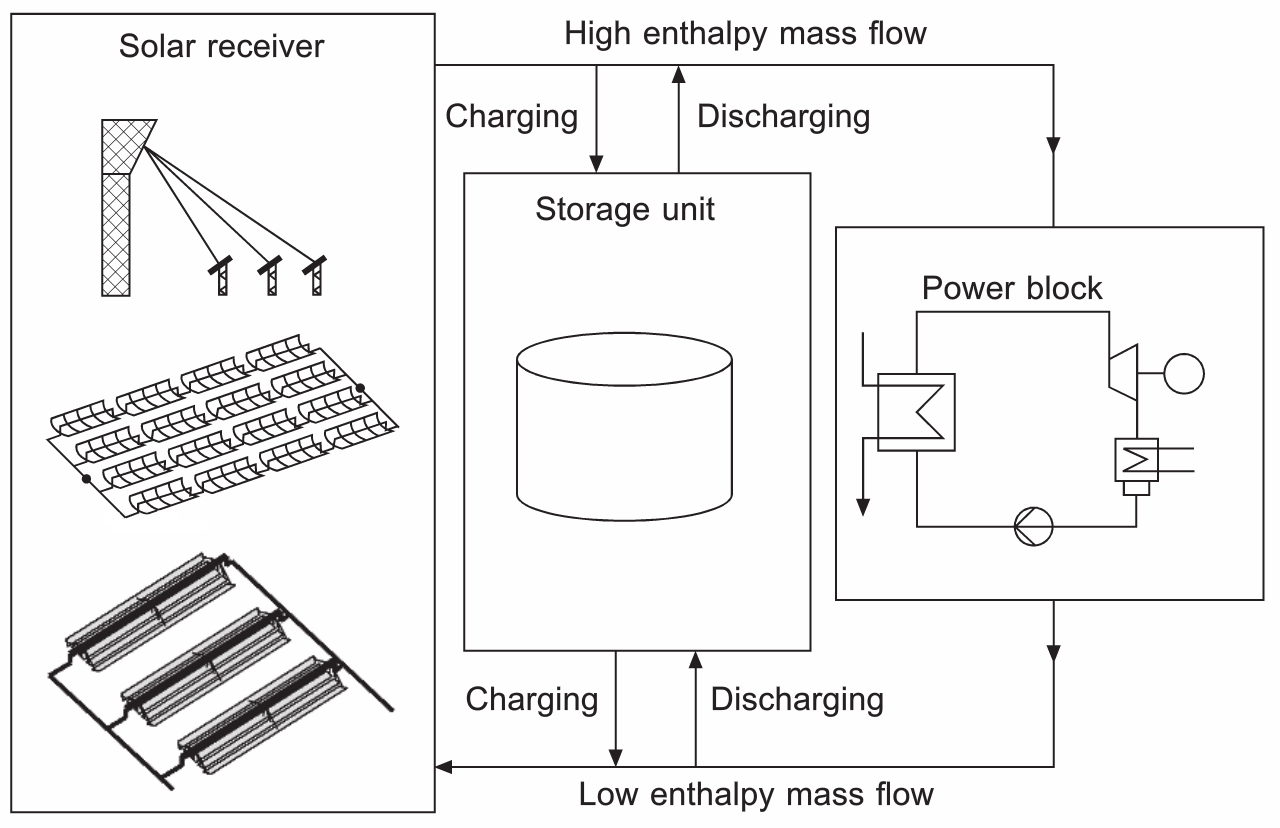
\includegraphics[width=0.70\linewidth]{FIG/integratedstoragescheme}
\caption[Scheme for CSP plant with integrated storage unit.]{Scheme for CSP plant with integrated storage unit \cite{Steinmann2015}.}\label{integratedstoragescheme}
\end{figure}
From a technical point of view, the storage must have high energy density, good heat transfer between the heat transfer fluid (HTF) and the storage medium, mechanically and chemically stable storage media, compatibility between the heat exchanger, heat transfer fluid and storage medium, complete reversibility, and minimum thermal losses. Actually, there are just four commercial used TES in CSP plants integrated (see below). But in generally a TES system, can store heat in the form of sensible, latent, or thermochemical energy. Latent and thermochemical based TES systems are still in the phase of research and development \cite{Steinmann2015}.
\begin{figure}[t]  
\centering
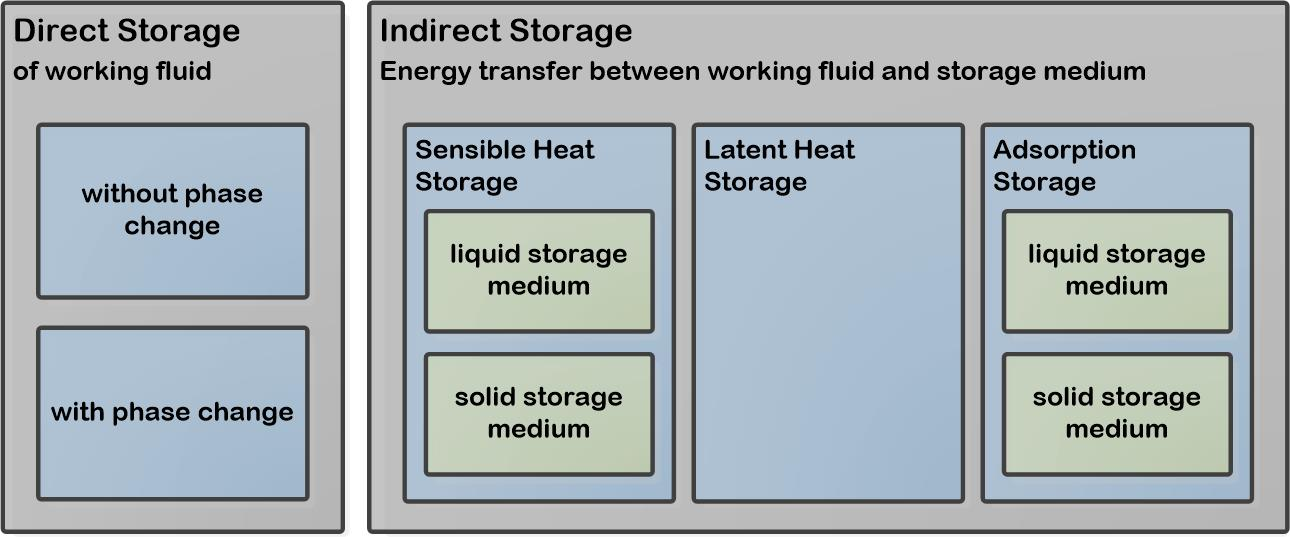
\includegraphics[width=0.75\linewidth]{FIG/Basicstorageconcepts}
\caption[Basic storage concepts for CSP systems.]{Basic storage concepts for CSP systems.}\label{Basicstorageconcepts}
\end{figure}
\\
In Figure~\ref{Basicstorageconcepts} is on one site the more basic concepts for a direct storage shown, which use the same working fluid for the storage system and the solar receiver and on the other site indirect systems transferring energy to a separate storage medium. The various storage concepts show different states of maturity. These commercial integrated storage systems and their application range will described in the following \cite{Steinmann2015}:
\begin{itemize}
\item Direct storage of heat transfer oil (Direct Storage of Liquid Working Fluid)
\item Indirect molten salt storage units (Indirect Storage in Liquid Media)
\item Steam accumulators (Direct Storage with Phase Change)
\item Direct molten salt storage units (Direct Storage of Liquid Working Fluid)
\end{itemize}
According to the "Technology Roadmap - Energy storage" of the International Energy Agency from 2014, alternative storage concept like heat storage with phase changing materials (PCM), thermochemical energy storage, and waste heat utilisation methods offer many potential opportunities. However, these technologies will need to overcome containment vessel design and material stability challenges at very high temperatures before they can achieve widespread deployment and will not further described or disused here. \cite{IEA2014e}\\
Likewise alternative concepts in liquid storage media such as dual media concepts (thermocline) and floating barrier concepts are still in the phase of research and development and will not be further described.\cite{Steinmann2015} \\
\\
In the following sensible liquid media will be described. Therefor the physical principles of heat storage systems are necessary. The amount of heat, $Q$ (in J), which can be stored in liquid sensible systems and the density, $E$ (J/m$^3$), related with this process can be calculated using the following equations:
\begin{align}
Q=m*C_p*(T_{out}-T_{in})=m*C_p*\Delta T \label{GL_heat}
\end{align}
\begin{align}
E=\rho*C_p*(T_{out}-T_{in})=\rho*C_p*\Delta T \label{GL_density}
\end{align}
where $T_{in}$ and $T_{out}$ are inlet and outlet storage system temperatures, respectively [K], $m$ is mass of storage liquid media [kg], $\rho$ is density [kg/m$^3$], and $C_p$ is specific heat capacity [J/(kg*K)]. Analyzing equation \ref{GL_heat} and \ref{GL_density}, it can be concluded that an optimum liquid sensible storage material must present high heat capacity, $C_p$, and a wide range of thermal stability, $\Delta T$. Different fluids have been studied as HTF and liquid sensible storage media \cite{Gil2010} and are shown in Table \ref{TableSensbleHeatStorageMaterial}. \cite{Ushak2015}
\begin{table}[h]
\centering
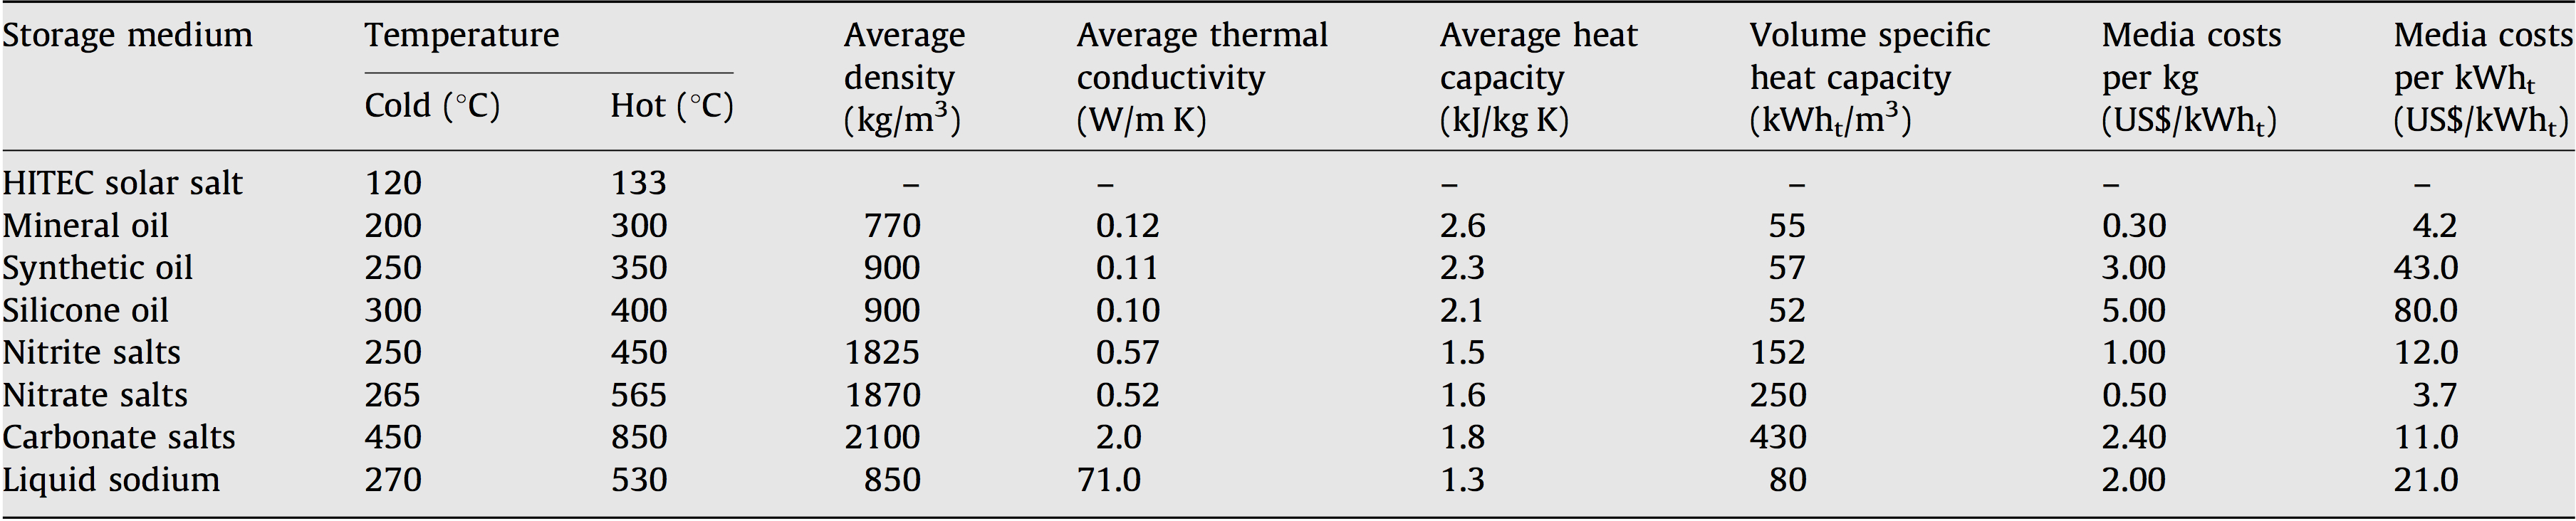
\includegraphics[width=1\textwidth]{FIG/TableSensbleHeatStorageMaterial}
\caption[Main characteristics of sensible heat storage liquid materials.]{Main characteristics of sensible heat storage liquid materials \cite{Gil2010}.}\label{TableSensbleHeatStorageMaterial}
\end{table}
\subsubsection{Direct storage of heat transfer oil}
The simplest concept to implement a TES into a CSP plant is the direct storage of the working fluid which is circulated through the solar absorbers. The first commercial used parabolic trough power plant SEGS-1, built 1984 in California, uses a mineral oil as heat transfer medium in the absorbers, which heats up from 240$\,^{\circ}\mathrm{C}$ to 305$\,^{\circ}\mathrm{C}$. The heat from the terminal oil was used to generate a power of 13.8~MW through the the Steam-electric power block. Two 4~700~m$^3$ carbon steel  tanks were used to separate the cold from the hot oil. This made a thermal storage capacity of 120~MWh$_{th}$ possible and allowed the system generate electricity for three hours. The storage system of the SEGS-1 was destroyed by a fire in 1999 and was not replaced. Figure~\ref{troughdirecttwotank} shows a simplified scheme of the SEGS-1 parabolic trough plant and their direct storage of heat transfer fluid. Mineral oil is today not considered to be an attractive medium for TES in large-scale CSP applications. The capital costs for large oil volume are substantial and needs additional investments for possible environmental hazards like oil leaks. Also the maximum operational temperature fore mineral oil is below 340$\,^{\circ}\mathrm{C}$, which restricts the efficiency of the thermal process. Present solar through power plants are using a synthetic heat transfer fluid whose costs are significantly higher (cf. Table \ref{TableSensbleHeatStorageMaterial}). Also increased the maximum temperature of the heat transfer fluid to 390$\,^{\circ}\mathrm{C}$ and needs a vapor pressure up to 10~bar at these temperatures, which is not able to storage stable at these conditions. All this made the direct storage of heat transfer oil not longer to the state of the art. \cite{Richter2013}\\
\begin{figure}[!ht]
        \centering
        \begin{subfigure}[b]{0.5\textwidth}
                \centering
                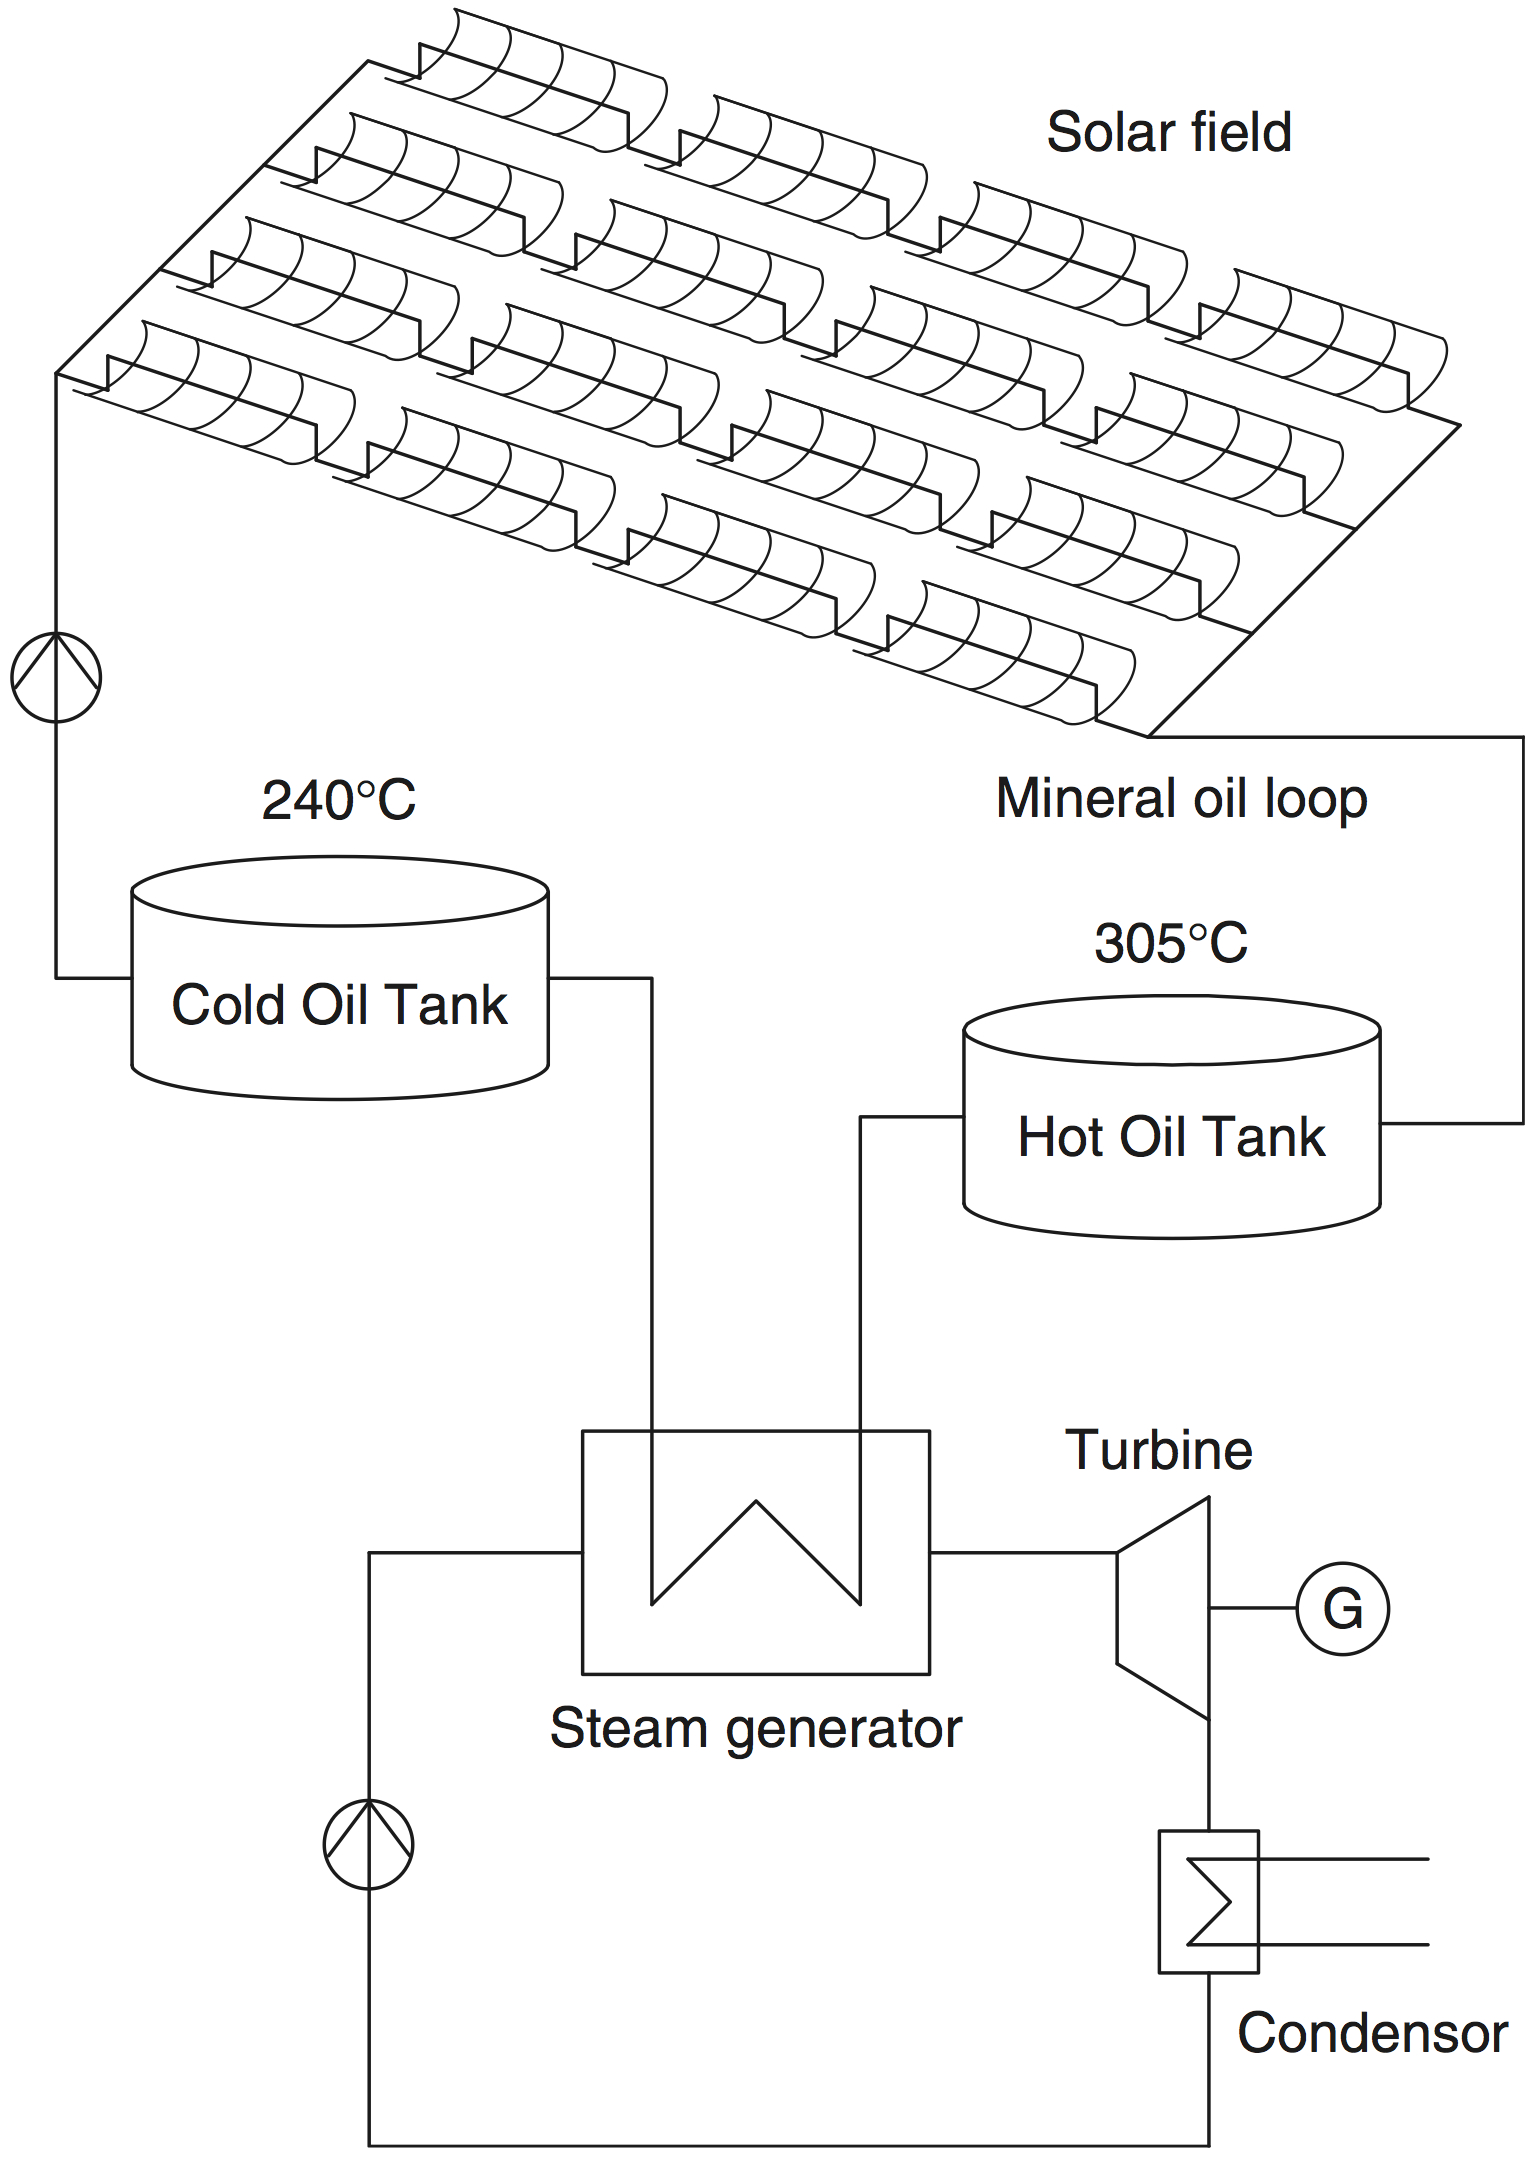
\includegraphics[width=0.6\textwidth]{FIG/troughdirecttwotank}
                \caption{SEGS-1 PTC plant with direct storage of heat transfer fluid.}\label{troughdirecttwotank}
        \end{subfigure}%
        ~
        \begin{subfigure}[b]{0.5\textwidth}
                \centering
                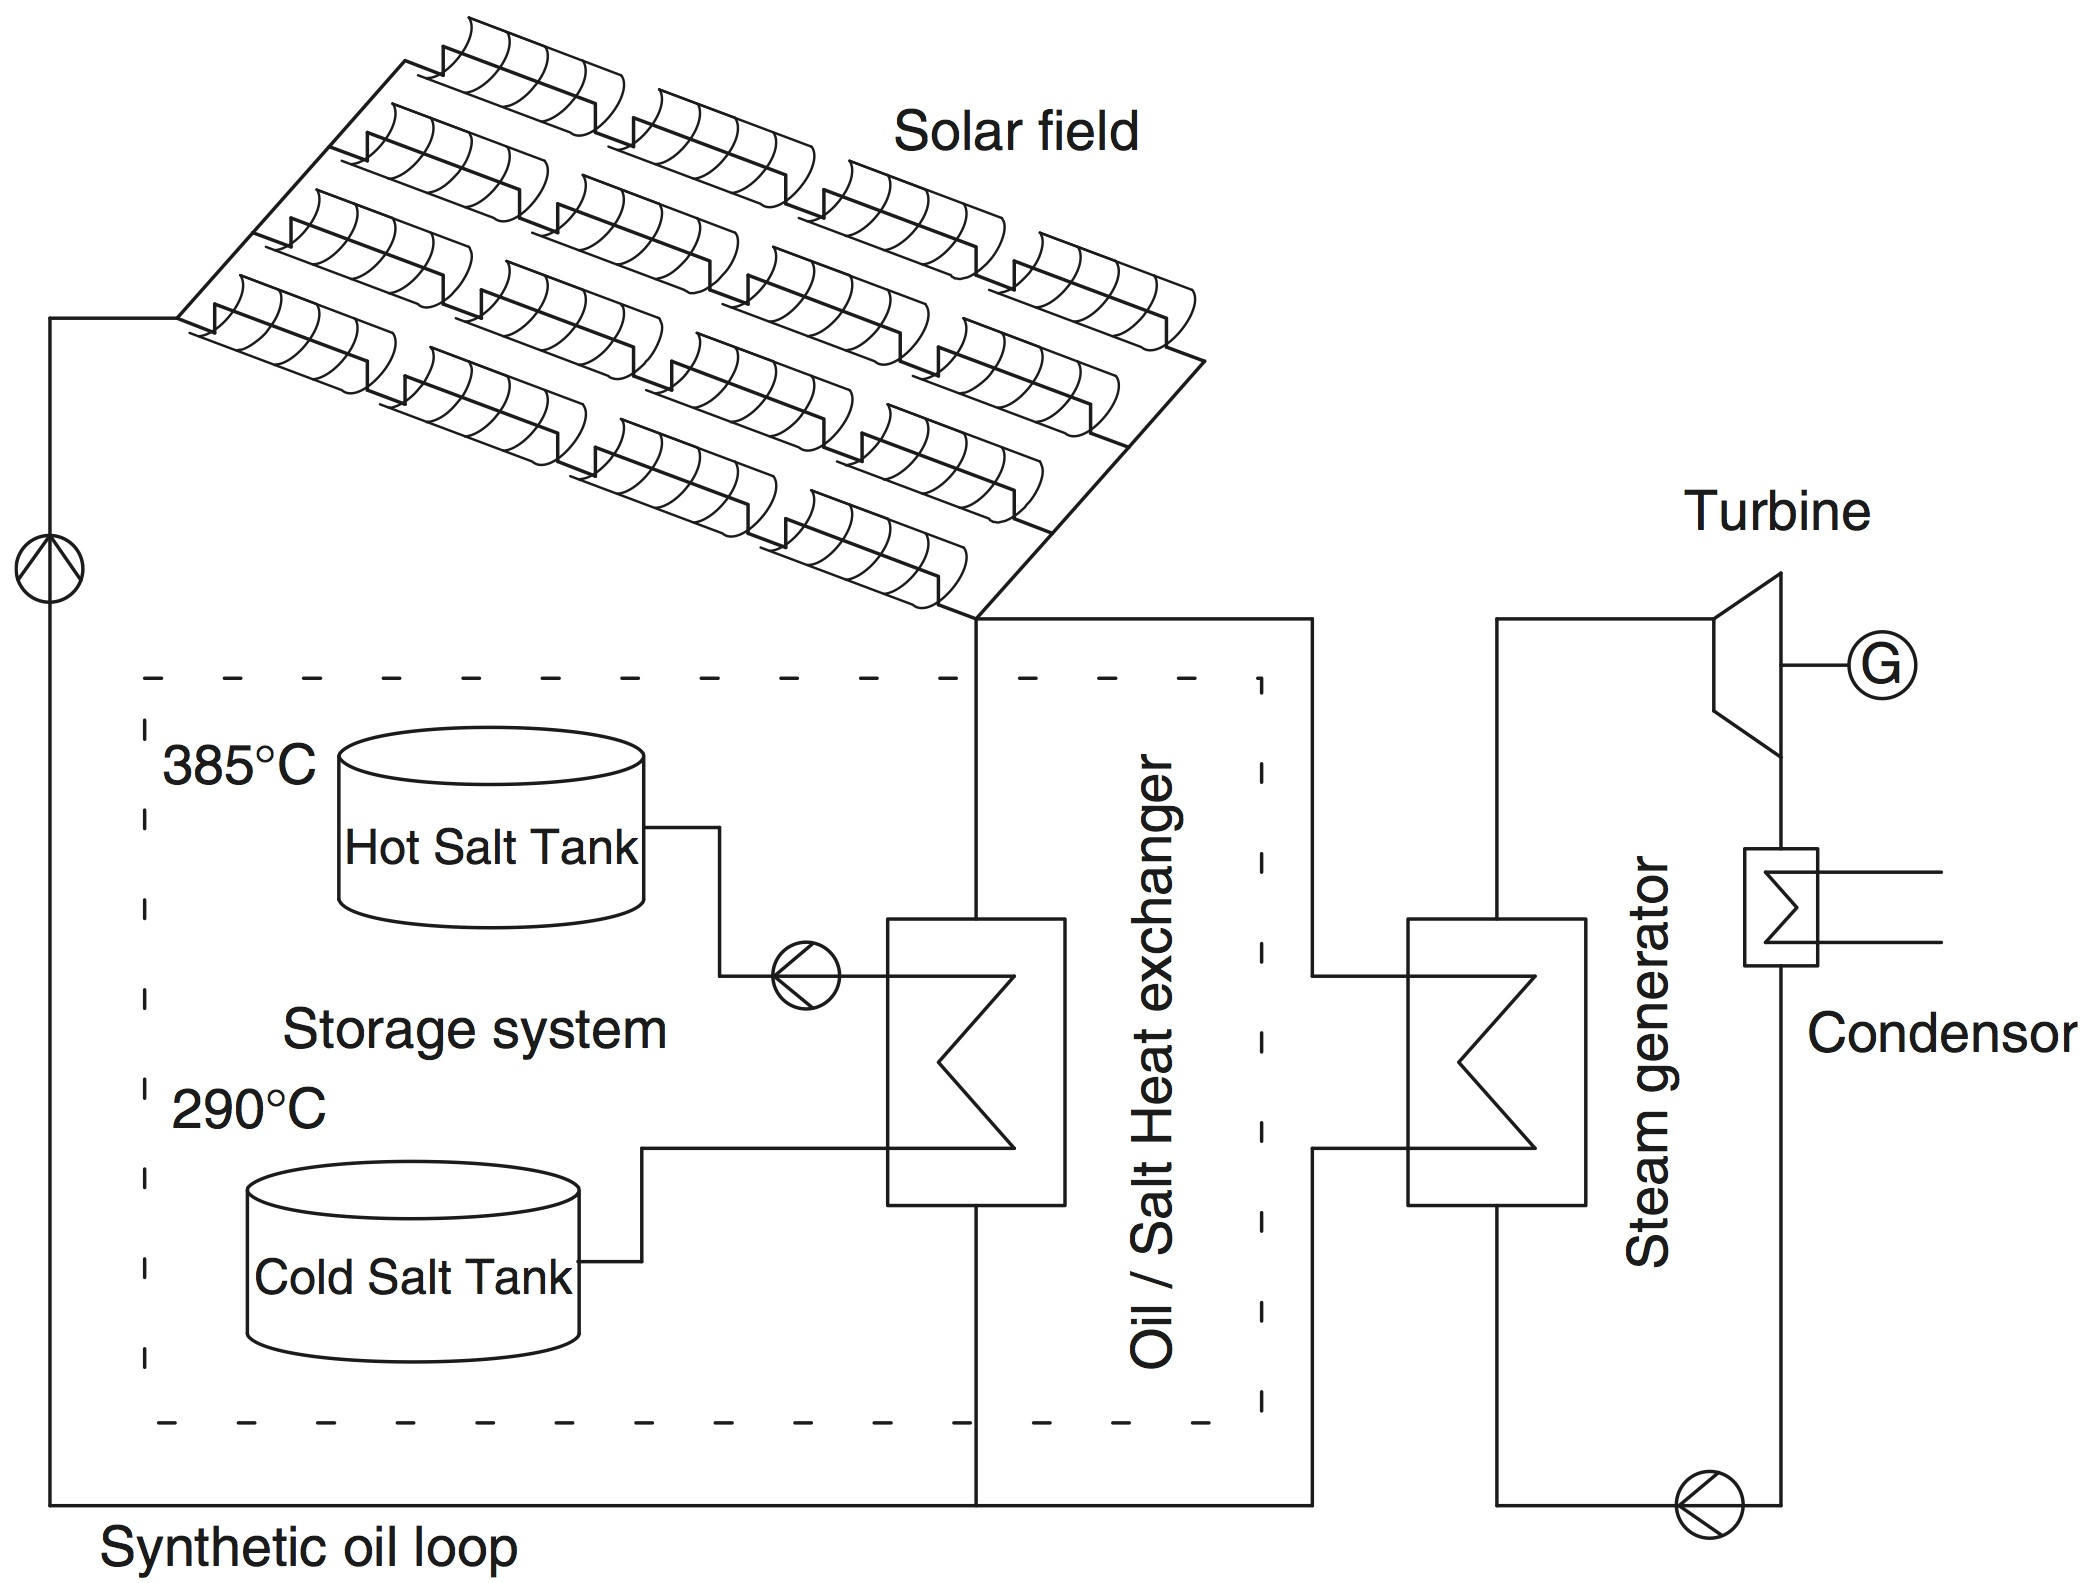
\includegraphics[width=1\textwidth]{FIG/troughtindirecttwotank}
                \caption{PTC power plant with indirect storage system using molten salt.}\label{troughtindirecttwotank}
        \end{subfigure}
        \caption[Simplified scheme of PTC power plants and storage concepts.]{Simplified scheme of PTC power plants and storage concepts \cite{Steinmann2012}.}\label{storageconceptstrough}
\end{figure}
\subsubsection{Indirect molten salt storage units}
Since the direct storage of the synthetic HTF is not attractive, an indirect storage concept was proposed. This should use a low cost storage medium, which can be stored at ambient pressure between 290$\,^{\circ}\mathrm{C}$ and 390$\,^{\circ}\mathrm{C}$. The use of molten nitrate salts was a nearby solution whose elements is considered and development since the early stage of CSP technology in the 1980's. Depending on the importance of material costs and there thermal stability, an sodium-nitrate-rich (NaNO$_3$) mixture containing 60\% NaNO$_3$ and 40\% KNO$_3$ (potassium nitrate) is preferred if an large quantities is required. The maximum temperature is in range of 550-580$\,^{\circ}\mathrm{C}$ and the melting temperature is in the range of 230$\,^{\circ}\mathrm{C}$. \cite{Richter2013}\\
Figure \ref{troughtindirecttwotank} shows a simplified scheme to implement a indirect two tank molten salt storage concept into a parabolic trough plant. Two separate insulated cylindrical thanks made of steel and carbon are used. Each tank can contain the total molten salt volume. Due to the temperature-dependent density of molten salt, the volume of the hot fluid tank has to be 4\% lager. To prevent freezing of molten salt an electrical immersion heaters are located at the bottom of the tanks.\cite{Kelly2006}.\\
The Andasol-1 facility, completed 2008 in Andalusia, Spain was the first commercial CSP plant using indirect molten salt storage. This plant can be operated for 7.5~h at 50~MW$_{el}$ by thermal energy provided by an indirect two-tank molten salt storage system. The molten salt storage fluid of 28~500~tons is cycled between 385$\,^{\circ}\mathrm{C}$ and 295$\,^{\circ}\mathrm{C}$, resulting a storage capacity of 1~050~MWh$_{th}$ \cite{Relloso2009}. The storage tanks have a height of 14~m and a diameter of 36~m. The similar CSP plants Andasol-2 and Andasol-3 started operation in 2009 and 2011. \cite{SolarMillenniumAG2008,NREL2008,NREL2013a,NREL2013}\\
Figure \ref{SolanaStorage} shows the Solana facility located in Arizona, USA. This plant was completed in 2013 and is the the largest parabolic trough plant so far. The indirect molten salt storage system uses 12 tanks to provide 280~MW$_{el}$ for a duration of six hours. \cite{AbengoaSolar2013a}\\
Since 2015 SA has also their first commercial CSP plant using indirect molten salt storage technology (Figure \ref{KaXu-solar-field}). KaXu Solar One is located next to Poffader in the Northern Cape and is a parabolic trough plant with 100~MW$_{el}$ capacity and 2.5~h of thermal storage in molten salts. \cite{NREL2015c}
\begin{figure}[!bhtp]  
\centering
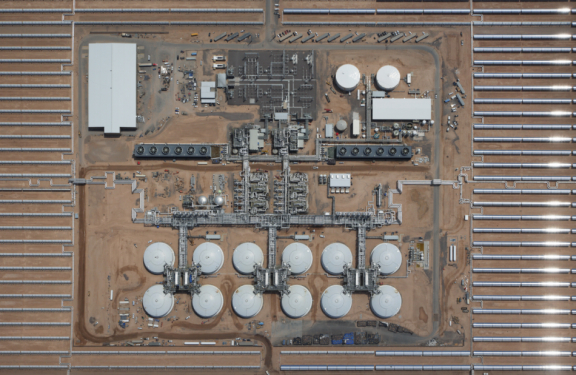
\includegraphics[width=0.9\linewidth]{FIG/SolanaStorage}
\caption[Overall view of Solana PTC facility with 12 storage tanks for molten salt.]{Overall view of Solana PTC facility with 12 storage tanks for molten salt \cite{AbengoaSolar2013}.}\label{SolanaStorage}
\end{figure}
\subsubsection{Steam accumulators}
In 2007 the first commercial CSP plant in Europe, the Planta Solar 10 (PS10) started near to Seville in Spain. The power tower uses saturated steam at 250$\,^{\circ}\mathrm{C}$ and 40~bar to drive a 11~MW$_{el}$ power circle. A schematic diagram of the PS10 is shown in Figure \ref{directsteamgeneration} on Page \pageref{directsteamgeneration}. The energy availability for storage is limited because the  plant is designed for a small solar multiple value of 1.3. Therefore a stream accumulator was selected as storage concept. The cross-sectional view of an steam accumulator is shown in Figure \ref{SteamAccumulatot}, which is also denoted as Ruths' storage or saturated steam storage. During charging the surplus stream is fed into a pressurized liquid water volume. The liquid water acts as storage medium. So the condensing steam increases the pressure and temperature of the liquid water in the volume. The storage is designed in horizontal cylindrical pressure vessel, whose volume is filled with 90\% saturated liquid and the remaining volume is filled by saturated stream. Saturated stream will provided during discharge by the steam accumulator. While the saturated steam is taken out of the steam accumulator is the pressure in the liquid volume declining. The saturated liquid volume generates thereby additional saturated steam by a reaction of the pressure reduction. Meanwhile the mass reduction of the liquid volume is usually in the range of 10-20\%. Pressure and temperature of the steam from the steam accumulator decline continuously during the discharge process. The PS-10 plant uses four separate tanks to store about 20~MWh$_{th}$ which is sufficient to produce 50\% load for 50 minutes. Attractive features of steam accumulators are their robustness and the simplicity of the concept. The fast reaction time makes the steam accumulator to an prefer storage concept of buffer storage solution intended for short fluctuation of solar radiation. But significant exergy losses occur due to the temperature difference between the steam and liquid volume during the charging. While steam accumulators are an attractive solution for small and medium sized solar process heat application, W.-D. Steinmann from the German Aerospace Center (DLR) \cite{Steinmann2015} has the opinion they are not expected to play a major role in the future of CSP applications. \cite{Richter2013}\\
Nonetheless the first power tower in SA, Khi Solar One will use super-heated steam, dry cooling technology, and a 2~h steam storage system. Khi Solar One is a 50 MW solar power tower plant being built by Abengoa near the town of Upington in the Northern Cape Province. Operation was scheduled to begin in 2014 but is still under construction (Status Oct. 2015). \cite{Abengoa2014,NREL2014}\\
\begin{figure}[!htbp]  
\centering
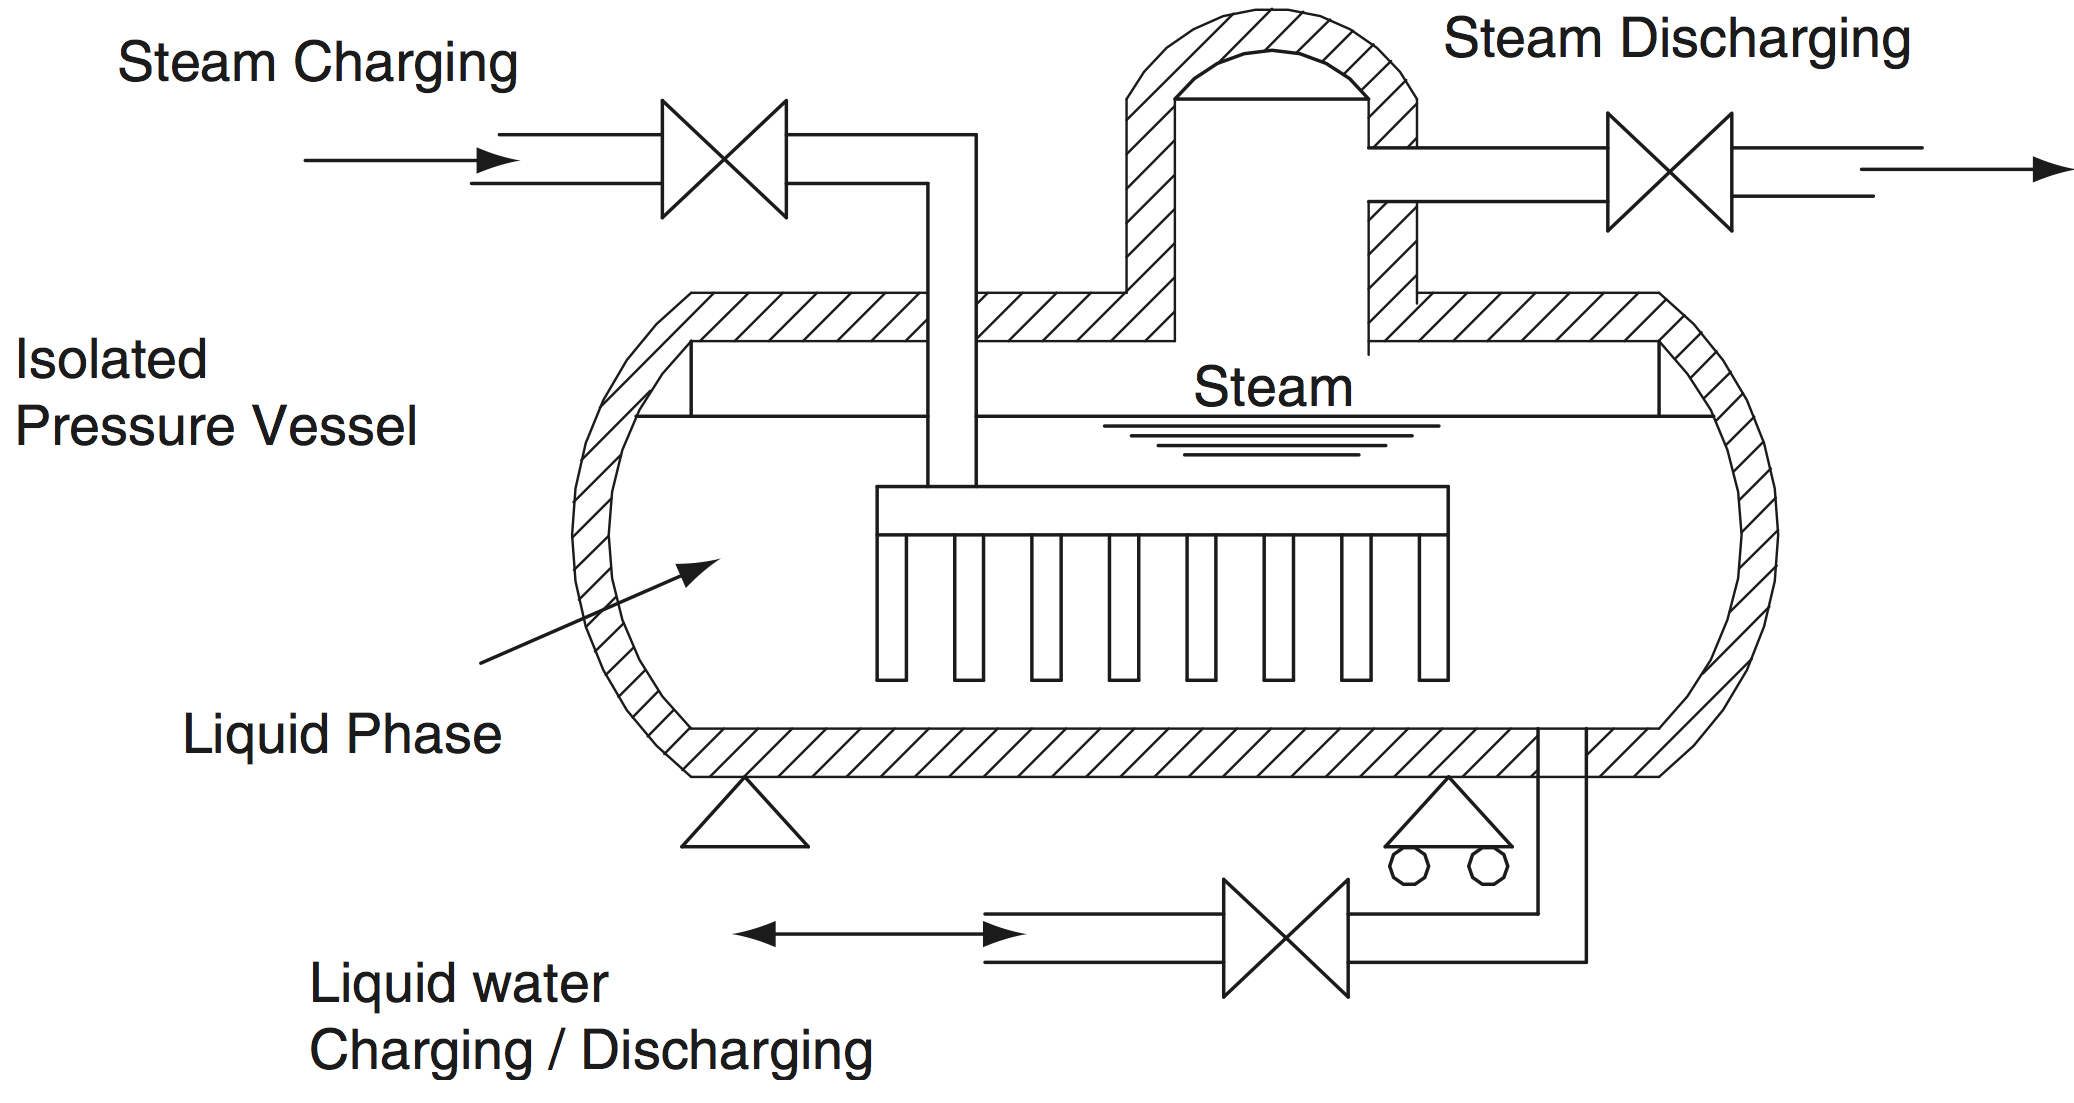
\includegraphics[width=0.7\linewidth]{FIG/SteamAccumulatot}
\caption[Scheme of a steam accumulator.]{Scheme of a steam accumulator \cite{Steinmann2006}.}\label{SteamAccumulatot}
\end{figure}
\subsubsection{Direct molten salt storage units}
Increasing the maximum process temperature of the thermal cycle of an CSP plant seams to be an efficient way to improve the economics of solar thermal electricity generation. A higher maximum process temperature allows also to increase the thermal storage cycle temperature, which has an significant impact on the specific storage capacity for sensible heat. Thereby the required storage inventory and the volume of the storage tanks can be reduced. Also less electric power for pumping the storage medium is required. But on the other hand, increasing with the higher temperature as well corrosion problems and thermomechanical stress.
\begin{figure}[t!]  
\centering
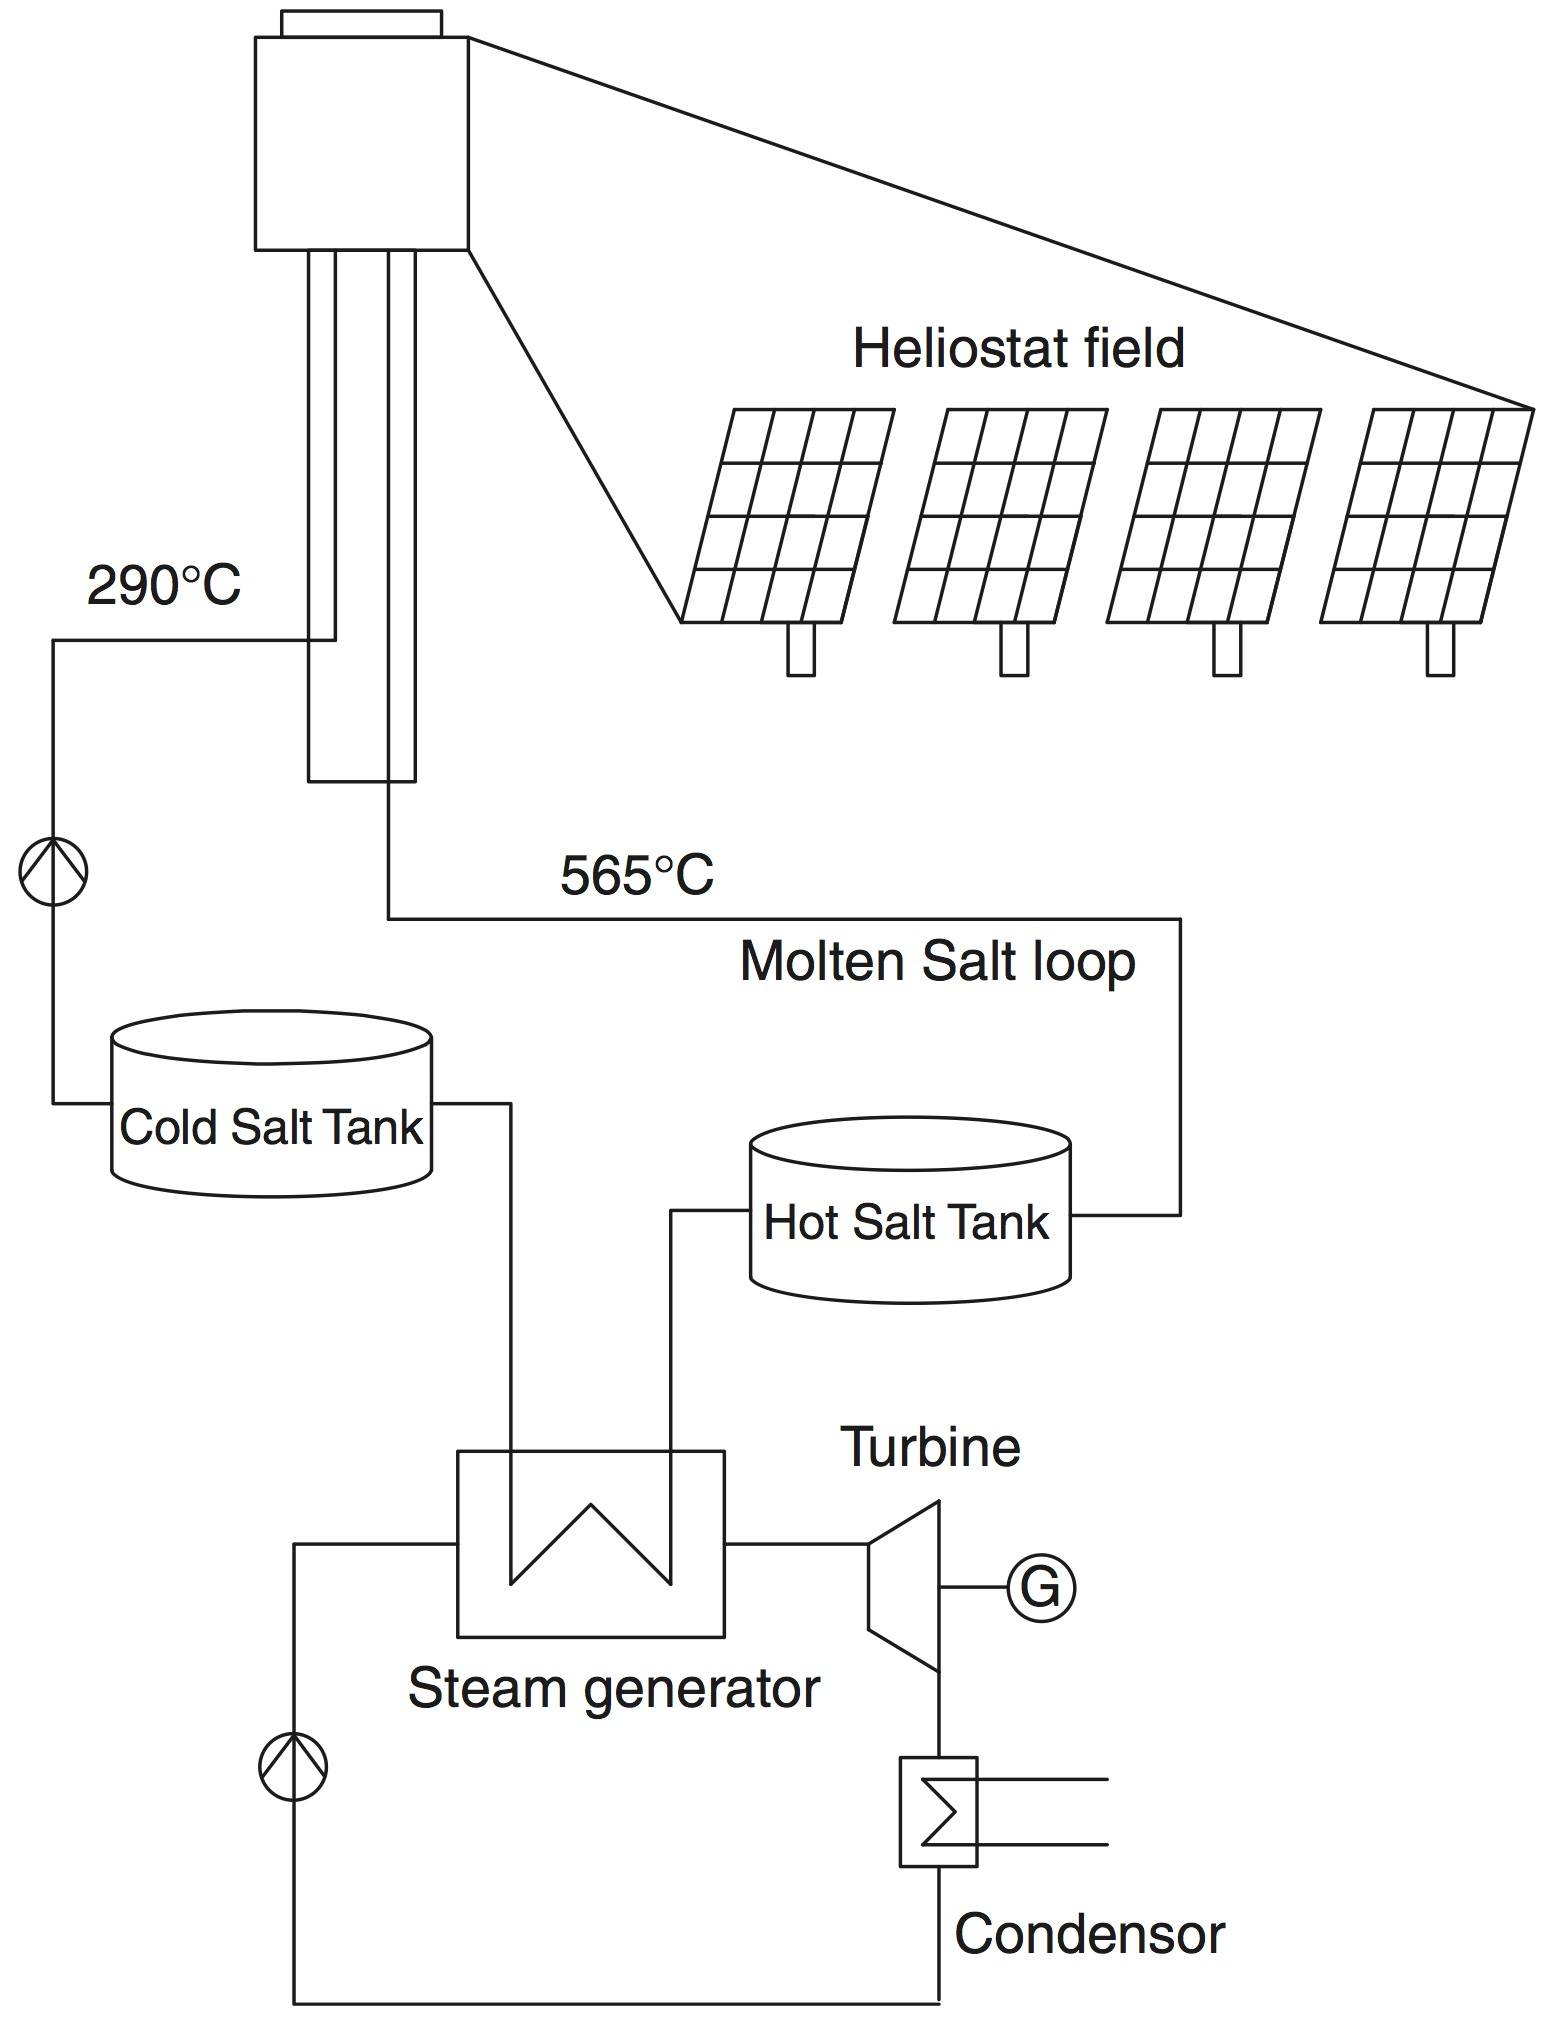
\includegraphics[width=0.45\linewidth]{FIG/towerdirecttwotank}
\caption[Simplified scheme of Solar Two CRS power plant with direct storage of molten salt used as heat transfer fluid.]{Simplified scheme of Solar Two CRS power plant with direct storage of molten salt used as heat transfer fluid \cite{Richter2013}.}\label{towerdirecttwotank}
\end{figure}
\\
Using the solar central receiver concept is an opportunity to raise the temperature of the process up to more than 565$\,^{\circ}\mathrm{C}$. Figure \ref{towerdirecttwotank}  shows a simplified scheme of direct two-tank molten salt storage concept integrated into CRS. This concept was first tested in the Solar Two power plant. This pilot solar-thermal project was built in the Mojave Desert just east of Barstow, CA, USA in 1994 on basis of the Solar One facility and was operating until 1999. A 10~MW$_{el}$ Rankine cycle was connected to the central receiver providing 35~MW$_{th}$. The two-tank storage system had an inventory of 1~400~t of a mixture of molten sodium nitrate (60\% by weight) and potassium nitrate (40\% by weight), with a total volume of about 1~700~m$^3$. The capacity of the storage system was 107~MWh$_{th}$ and operated between 565$\,^{\circ}\mathrm{C}$ and 290$\,^{\circ}\mathrm{C}$, which allowed the operation of the turbine for 3~h. The external isolated tanks had both a diameter of 11.6~m, the hot tank was mad of stainless steel had a height of 8.4~m with thermal loss in the range of 100~kW, the cold tank made of carbon steel was 7.8~m tall and transferred about 50~kW to the environment. The Solar Two project also gained the operational experience for handling larger quantities of nitrate salt for storage applications. Although, their was some changes observed in the physical properties of molten salt during the duration of the project, their was no problems resulted. After the 30~000~h project test and the analyses of the construction material, it was concluded that salt-induced no practical limitation on the useful life of tanks. Also the nitrate salt was recycled for use as fertilizer at the end of the project. \cite{Steinmann2015} \\
The first commercial solar tower plant using molten salt with a direct storage system is Gemasolar, which was commissioned in 2011. It uses the first high-temperature solar receiver with molten salt, which provides 15 hours of thermal storage and an annual capacity factor of about 75\%. The size of the storage allows the plant to operate 24~h per day. The facility generates 19.9~MW$_{el}$ from 2~650~heliostats each 120~m$^2$ aperture area. The technology is based on the Solar Two and has the same temperature difference in the receiver from 275~K. \cite{NREL2011}\\
The Atacama-1, which is currently under construction in the Atacama desert in Chile, will also use a direct storage in molten salt for 17.5~h of storage. \cite{NREL2015b,AbengoaSolar2015a,AbengoaSolar2015}\\
Also parabolic trough power plants using direct molten salt storage units. The commercial used Archimede solar power plant in Italy is the first parabolic trough plant using molten salt as HTF. It started 2010 the production with 5~MW turbine capacity. The storage capacity reaches for 8 hours and has a total mass of 1~580~t of molten salt. With a tank size of 6.5~m in height and 13.5 m in diameter, the capacity is 100~MWh$_{th}$. \cite{NREL2012}\\
\\
In a nutshell, the direct or indirect two-tank molten salt storage technologies are represent current state of art for commercial large-scale CSP applications. While this concepts shows a low technical and environmental risk, the potential for cost reduction is limited here. 
\subsection{Power cycles for CSP systems} \label{subsection_powerblock}
As mentioned in the overview of solar power technologies in Figure \ref{OverviewSTP} on Page \pageref{OverviewSTP}, a range of different solar to electric energy conversion systems can be applied. Commonly used as conversion systems in current large-scale CR and PTC applications are steam turbines which are based on the Rankine cycle. Nearly all convectional fired power plants using the Rankine cycle to convert heat in electricity. If an conventional fired combined cycle power plant is supplemented with a CSP system it uses an integrated solar combined cycle (ISCC), which is also based on the Rankine cycle. An additional conversion systems for CRS and parabolic dishes is the Brayton cycle (also known as Joule cycle). However, for efficient cycle operation temperatures of 1~000$\,^{\circ}\mathrm{C}$ are needed. Therefore the Brayton cycle has just been operated in demonstration CSP systems. CSP systems also uses Organic Rankine cycles, Stirling engines and other opportunities to generate electricity. \cite{Lovegrove2012}\\
\\
A CSP plant with Rankine cycle is basically working in four steps using a steam turbine:
\begin{itemize}
\item Compressing pure feed water to high pressure. 
\item Pre-heating, boiling and superheating steam in a boiler which may be in the focal point, or may be heated using a heat exchanger with another HTF. 
\item Expanding the steam to low pressure via a series of turbines that drive a generator.
\item At the end of the expansion process, condensing the low pressure steam, with the aid of a cooling tower and then re-using it in the cycle.
\end{itemize}
\newpage
\section{Large scale PV power plants}\label{Large scale photo voltaic (PV) power plants}
two axis tracking PV
\subsection{Large-scale PV power plants}

\subsection{Large-scale electrical energy storage systems}
electrical energy storage (EES)
EESSchema
\begin{figure}[htbp]  
\centering
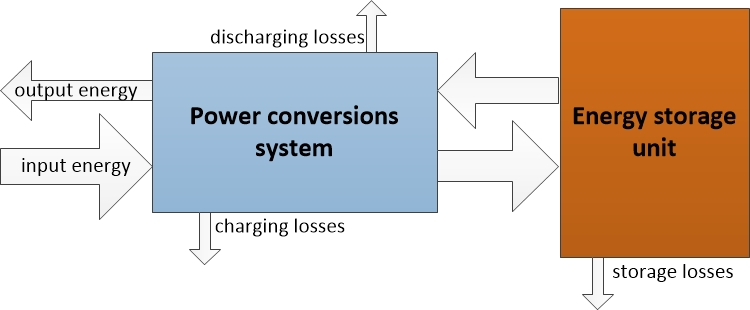
\includegraphics[width=0.65\linewidth]{FIG/EESSchema}
\caption[Schema of an electrical energy storage (EES) system and there energy losses.]{Schema of an electrical energy storage (EES) system and there energy losses.}\label{TCC_EES}
\end{figure}

\begin{equation}
\textrm{Overall storage efficiency (AC-to-AC)} =\frac{E_{out} \textrm{ (kWh)} }{E_{in} \textrm{ (kWh)}}
\end{equation}

\begin{figure}[htbp]  
\centering
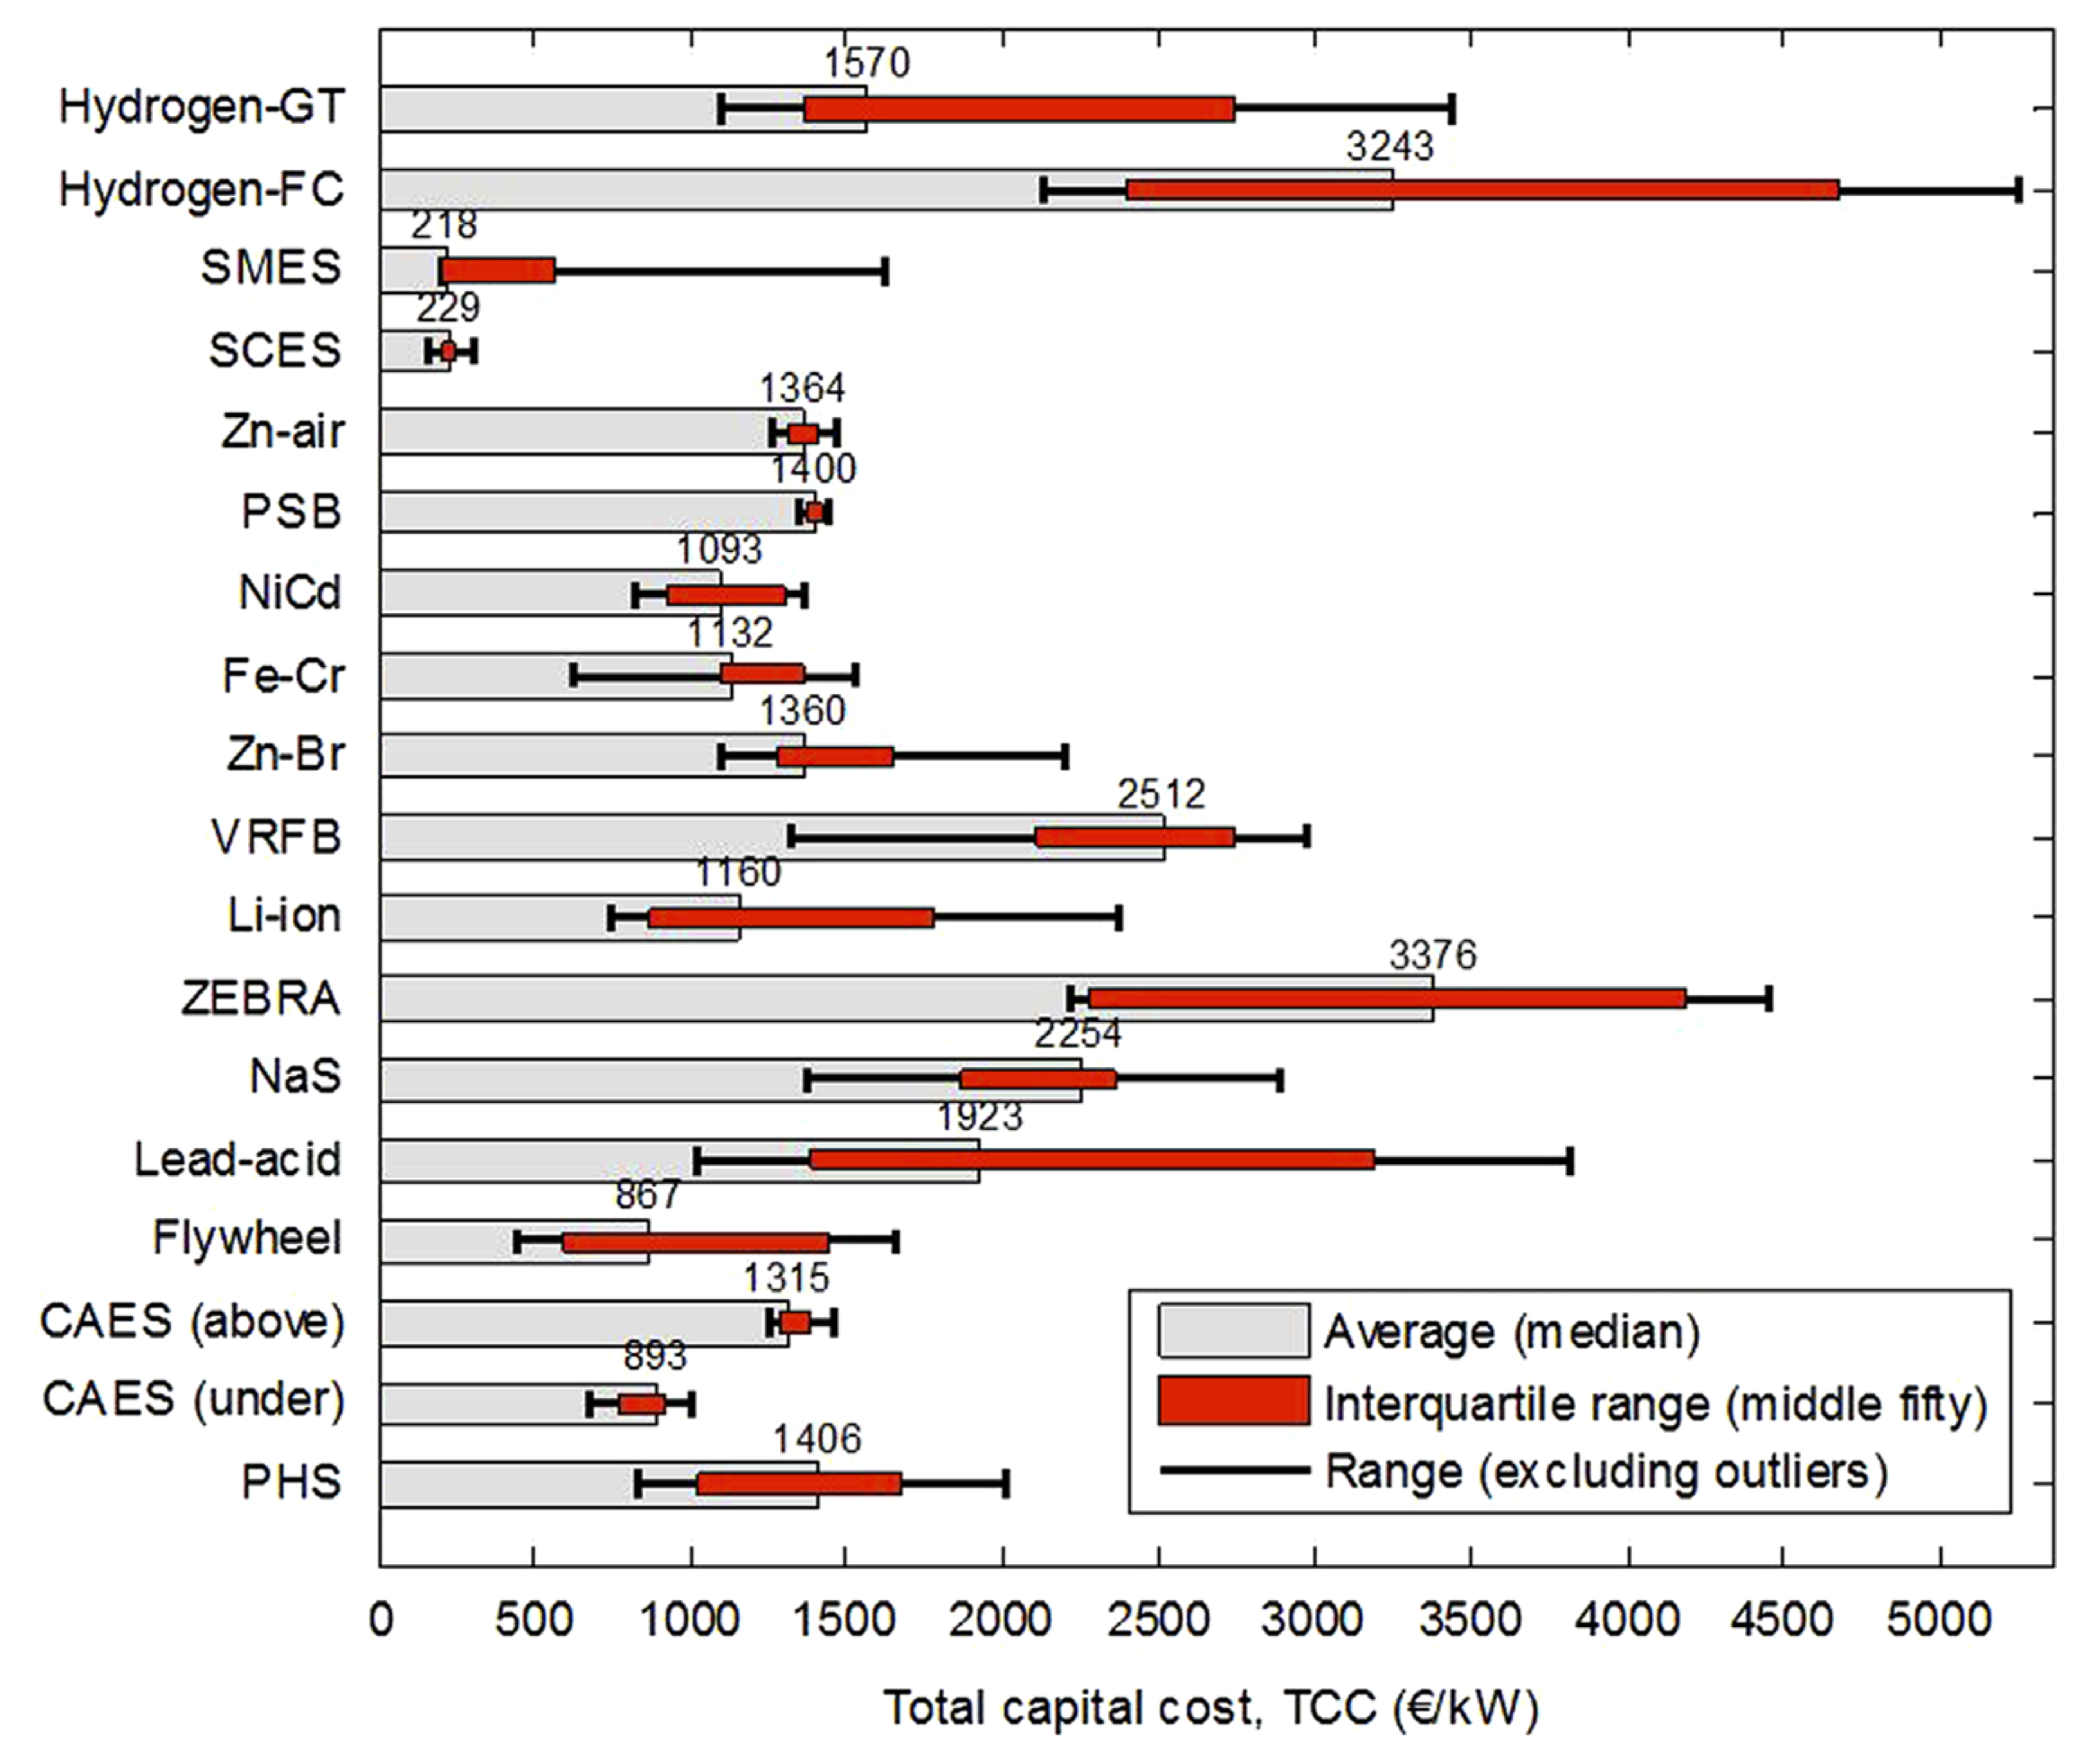
\includegraphics[width=0.75\linewidth]{FIG/TCC_EES}
\caption[Total capital cost in Euro (€) of large-scale EES systems per unit of nominal power rating including costs of power electronics, storage part, fixed obtain and maintainence and maybe incidental replacement costs.]{Total capital cost in Euro (€) of large-scale EES systems per unit of nominal power rating including costs of power electronics, storage part, fixed obtain and maintainence and maybe incidental replacement costs \cite{Zakeri2015}.}\label{TCC_EES}
\end{figure}

\section{Environmental impacts of CSP and PV}
Co2\\
Water use in O \& M\\
land use\\
energy use in operation and building
\cite{EASAC2011}\\
\cite{Caldes2012} \\
\section{Chapter summary}

\pagebreak
\chapter{Simulation-based comparison between CSP- and PV-power plants}
The aim of this chapter is to compare the technologies of the CSP system with a PV system. The comparison a CR system and a PTC system was simulated. Special attention was paid in this comparison for a high run time of the system during the day and the covering of a prescribed demand curve. For this comparison the PV system was expanded with an electrical energy storage. For the simulation an battery storage was selected. The dimension of the stored energy in this simulation went much beyond the actual technical capacity of individual electrical storage units and reaches more than one-sixt of the actual world battery storage capacity 690~GW \cite{IEA2015}. Therefor must be said at this point that this is a theoretical comparison from the viewpoint of the PV, in particular for this plant and storage scale.
\pagebreak
\section{General acceptance of conditions}
With the aim of producing quantifiable and comparable results, the different solar supplied power plants will be simulated under different input  parameters. After that, chosen comparable output parameter will be analyzed, evaluated and rated.

The for the comparison selected solar supplied power plants technologies are: 
\begin{itemize}
\item CSP molten salt central receiver with thermal energy storage
\item CSP synthetic oil parabolic trough with thermal energy storage
\item PV fixed elevated flat plate collectors with adapted electrical energy storage
\end{itemize}
As mentioned before the PV system got extended with a electrical energy storage (EES) for the simulation. There are various EES options. For the simulation the EES is based on the Li-Ion technology. The thermal energy storages of the CSP plants are based on the molten salt technology.\\
\\
All power plants got laid out for a maximum power output of 100~MW$_{el}$. For the comparison the power plants are forced to cover a selected load scenario. In order to find an individual suitable power plant design to cover the scheduled output of the scenario, different layout conditions, using various storage and collecting field sizes, was tried. The scenario and there goals are discussed and defined in Section~\ref{Overall simulated configuration}. The location and related weather data is defined in Section~\ref{Location and weather data}.\\
\\
The solar power plants are implemented and simulated in NREL’s System Advisor Model (SAM) version SAM 2015.6.30 r3 for OS X \cite{NREL2015}. SAM is designed to simulate performance and financial models of different types of renewable energies. For the simulation the performance part of the software was used. The financial analysis was made separately. \\
\\
The financial parameters and the resulting levelized cost of electricity (LCOE) are calculated separately  for all power plants in Microfoft Excel 2011 (vers. 14.5.7) for Mac using a simplified method which is documented in Appendix~\ref{ChapterLCOE} on Page \pageref{ChapterLCOE} using a lifetime of 25~years for each power plant.
\subsection{Overall simulated scenario} \label{Overall simulated configuration}
Power plants are forced to supply the system load/demand. Figure~\ref{LoadScenarios} shows the daily average system load/demand in South Africa for the winter and summer period. The profiles from both load shapes rises at approx 7:00 in the morning and has there peak demand at 20:00 during the summer period. During the winter period the first peak is reached at 9:00 in the morning and the other one at 19:00 in the evaning. In order to supply this system load the simulated solar power plants are forced to generate full power output of 100~MW from 7:00 to 22:00. When the system demand comes down during the night also the power plants reduce there output from 22:00 to 7:00 to 50~MW. The scenario is called "night-reduction".
\begin{figure}[htbp]  
\centering
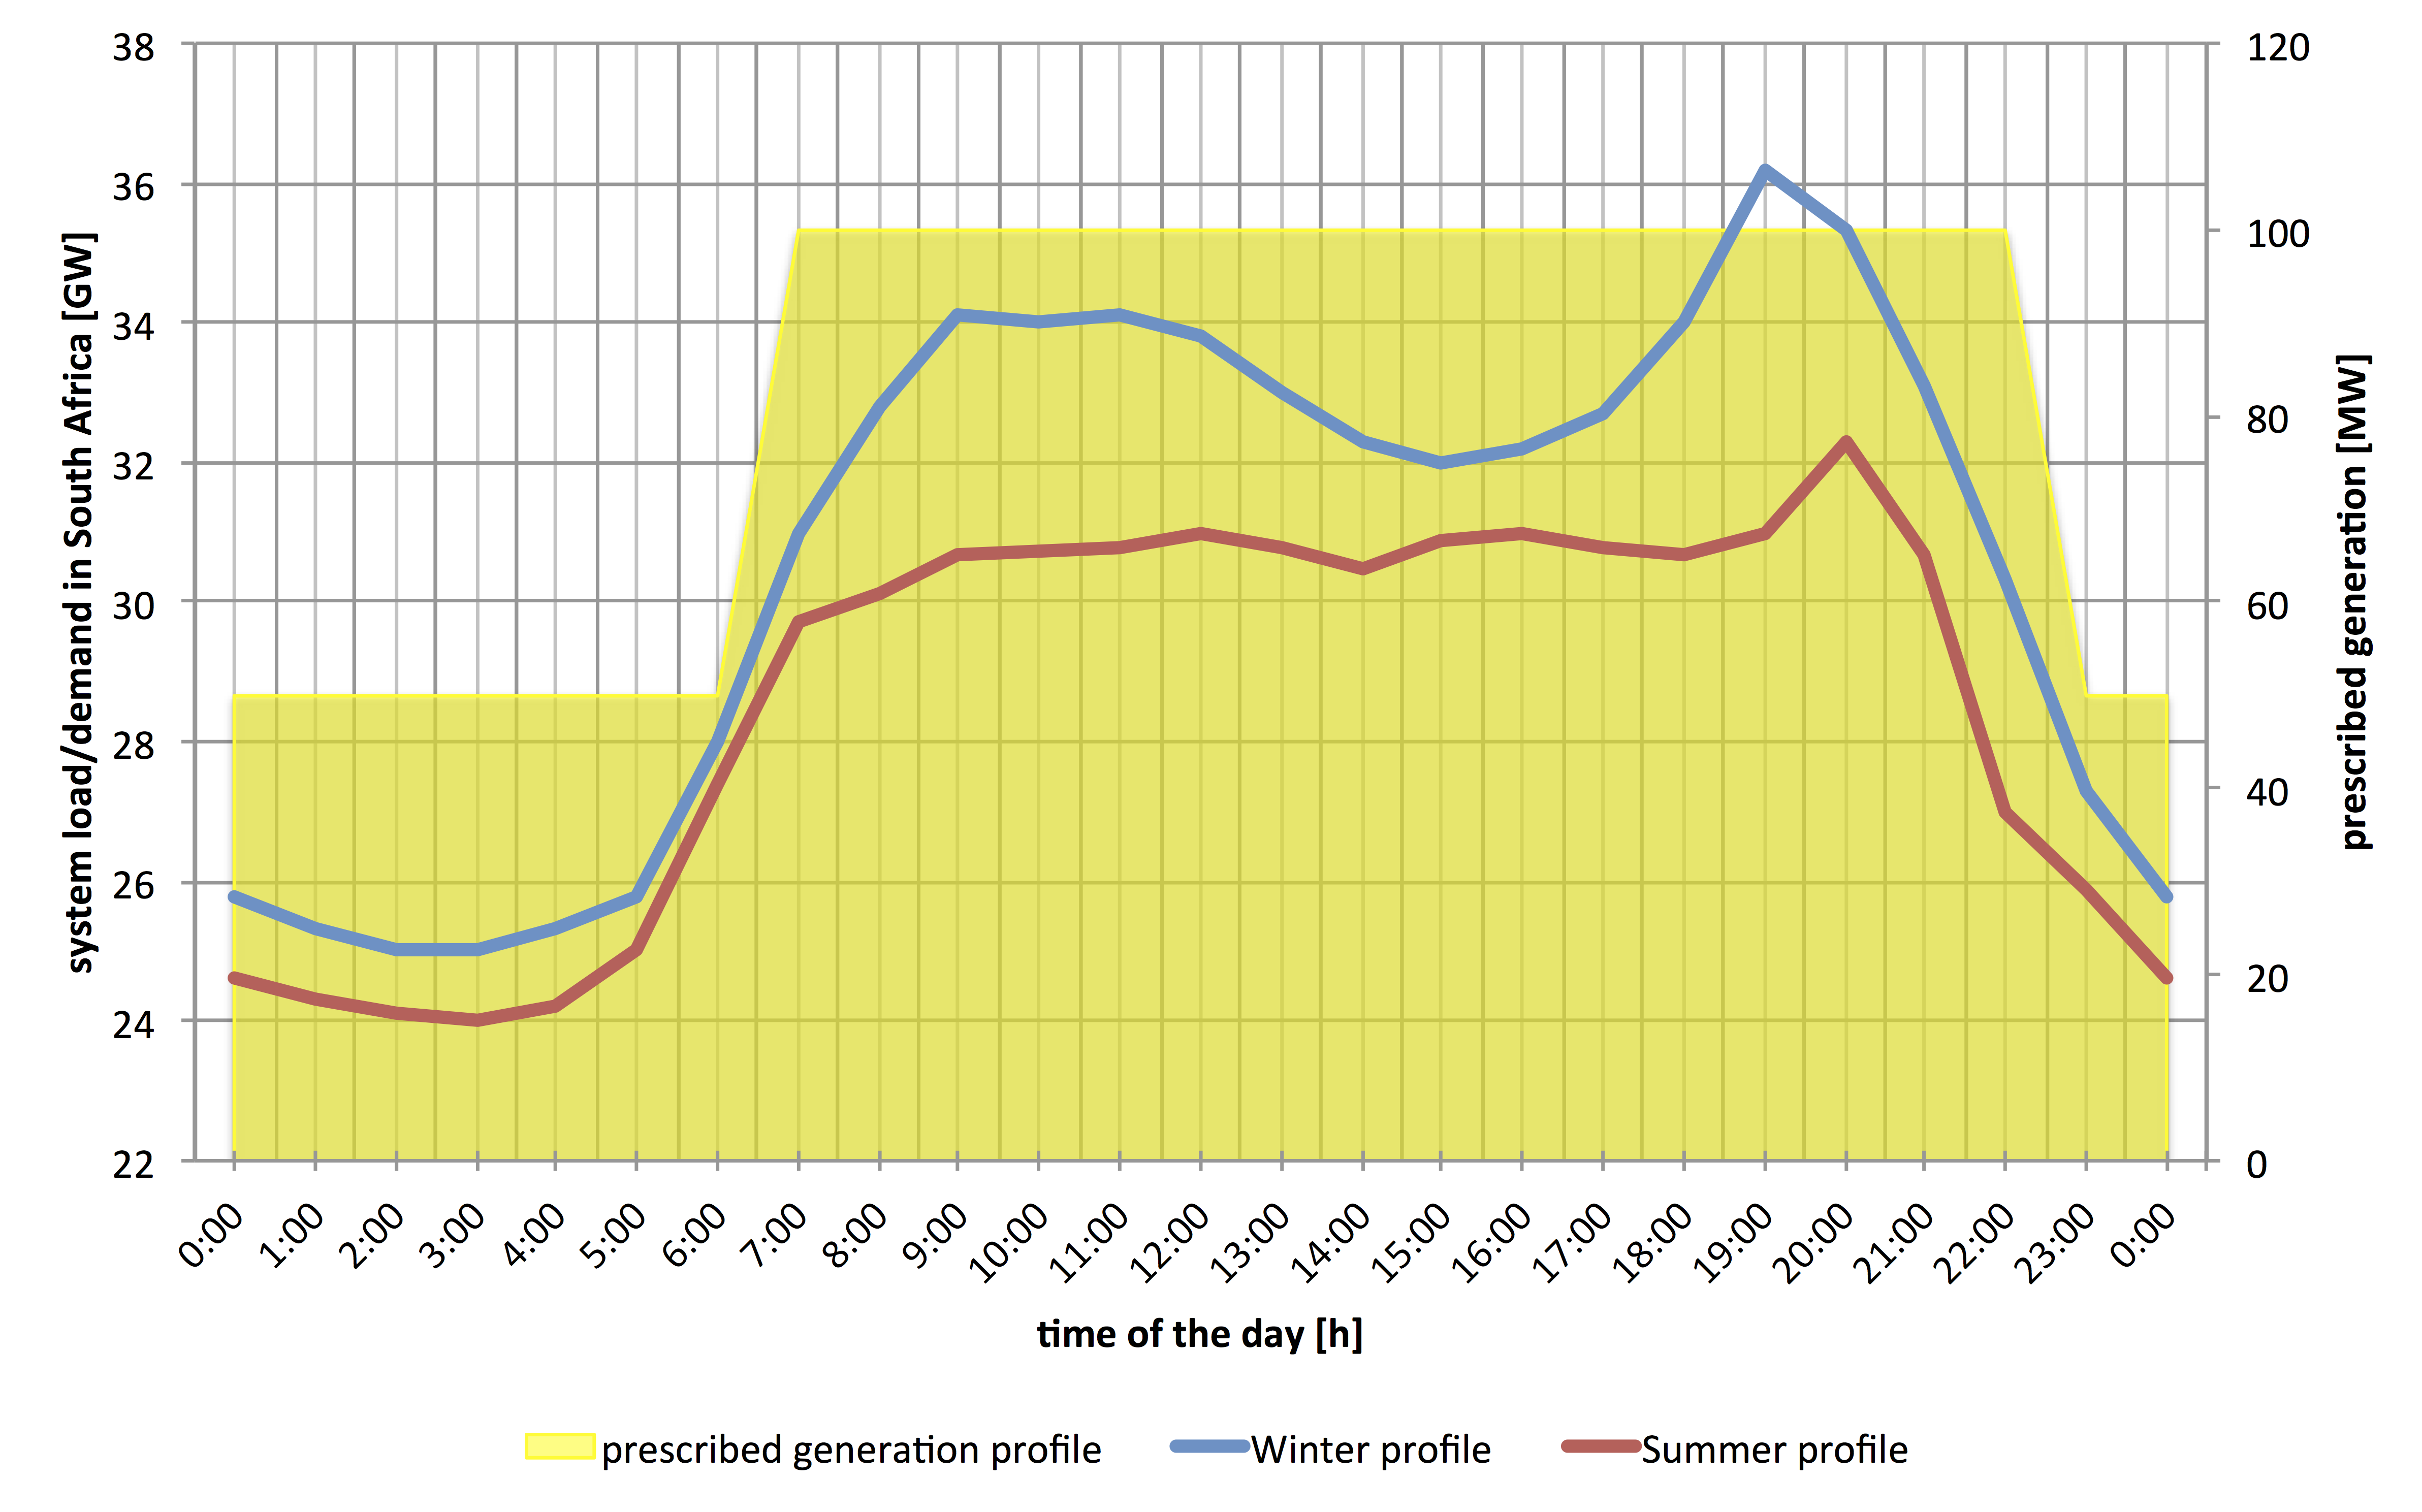
\includegraphics[width=1\linewidth]{FIG/LoadScenarios}
\caption[South Africas daily average system load/demand for summer and winter days, with sheduled power production curve.]{South Africas daily average system load/demand for summer and winter days, with sheduled power production curve.}\label{LoadScenarios}
\end{figure}
For the comparison the power plants there system design is forced to cover 90~\% of the scheduled electricity production over the first year.  Usually, in feed-in contracts the power output is fixed at specified values. The overproduction is not content of these contracts and is not remunerated. In order to generate exploitable and comparable results and also considering the common feed-in contracts for power plants, the hourly power production is cut to the planed values. So overproduction will not considered in the evaluation and analyses of the systems.\\
The results of the simulated scenarios and the financial analyses will be rated in two selected categories:
\begin{itemize}
\item \textbf{Load curve covering factor} [\%]: The Load curve covering factor (LCCF) describes quantitative how effective the power plant follows the required load curve of the scenarios.
\item \textbf{Levelized cost of electricity} [\textcent /kWh]: The levelized cost of electricity (LCOE) represents the total project lifecycle costs. It is the present value of project costs expressed in cents per kilowatt-hour of electricity generated by the system over its life. \cite{NREL2015a}
\end{itemize}
There is a huge difference between the mentioned LCCF and the widespread capacity factor (CF). The CF is the ratio of the system's predicted electrical output in the first year of operation to the nameplate output, which is equivalent to the quantity of energy the system would generate if it operated at its nameplate capacity for every hour of the year \cite{NREL2015a}. As it is mentioned above is the LCCF calculated from the sum value of load covering in each hour of the year.
\subsection{Location and weather data} \label{Location and weather data}
For the simulation of the solar power plants the locations and weather parameter of Upington, Northern Cape was used. This location is situated in a region with one of the highest irradiation values of the country, but also has a good water access by the Orange River. This locations was mentioned before in Chapter~\ref{Solar power in South Africa} and is marked in the GHI- and DNI-maps of SA in Figure \ref{irradiation} on Page \pageref{irradiation}. 
\begin{table}[!h]  
  \centering
	\begin{tabular}{  p{4.0cm}  C{4.0cm}  C{3.0cm} } 

	\hline	
\textbf{Item}  & \textbf{Value} & \textbf{Unit} \\ \hline \hline
Location & Upington & -\\ 
Station ID &  684240& -  \\ 
Data source & White Box Technologies, Inc. (31.05.2015) & -\\ \hline
Latitude & -28.40 &$\,^{\circ}$N \\ 
Longitude &  21.27 &$\,^{\circ}$E \\ 
Elevation &  836 & m \\ 
Total GHI per year  &  2~280 & kWh/m\textsuperscript{2}\\ 
Total DNI per year &  2~621 & kWh/m\textsuperscript{2}\\ 
Total DHI per year &  516 & kWh/m\textsuperscript{2}\\ 
Mean temp. &  21 & $\,^{\circ}\mathrm{C}$\\ 
Mean wind speed & 3.3 & m/s\\ \hline
\end{tabular}
\caption[Location and their characteristics for the simulation in SAM.]{Location and their characteristics for the simulation in SAM.}\label{tbl: Location}
\end{table}
\\
The input weather data for the simulation with SAM are in the EPW-format (EnergyPlus Weather Data) and produced by White Box Technologies, Inc. \cite{WhiteBoxTechnologies2015}. The EPW-files are data sets of hourly values of solar radiation and meteorological elements for a typical one-year period. This includes air temperature, dew point temperature, relative Humidity, atmospheric pressure, global horizontal solar radiation, diffuse Horizontal solar radiation, direct normal radiation, wind Speed, wind Direction and cloud cover. The for the simulation most relevant values are summarized in Table \ref{tbl: Location}. The hourly values of global horizontal and direct normal irradiance from the EPW-file is shown in Figure~\ref{Upington_GHI/DNI}. The highest irradiance value during the summer time is 1~199~Wh/m\textsuperscript{2} for GHI and 1~154~Wh/m\textsuperscript{2} for DNI. At the shortest day the highest irradiance is 625~Wh/m\textsuperscript{2} for GHI and 820~Wh/m\textsuperscript{2} for DNI.\\
\begin{figure}[!htbp]
        \centering
                \begin{subfigure}[b]{1\textwidth}
                \centering
                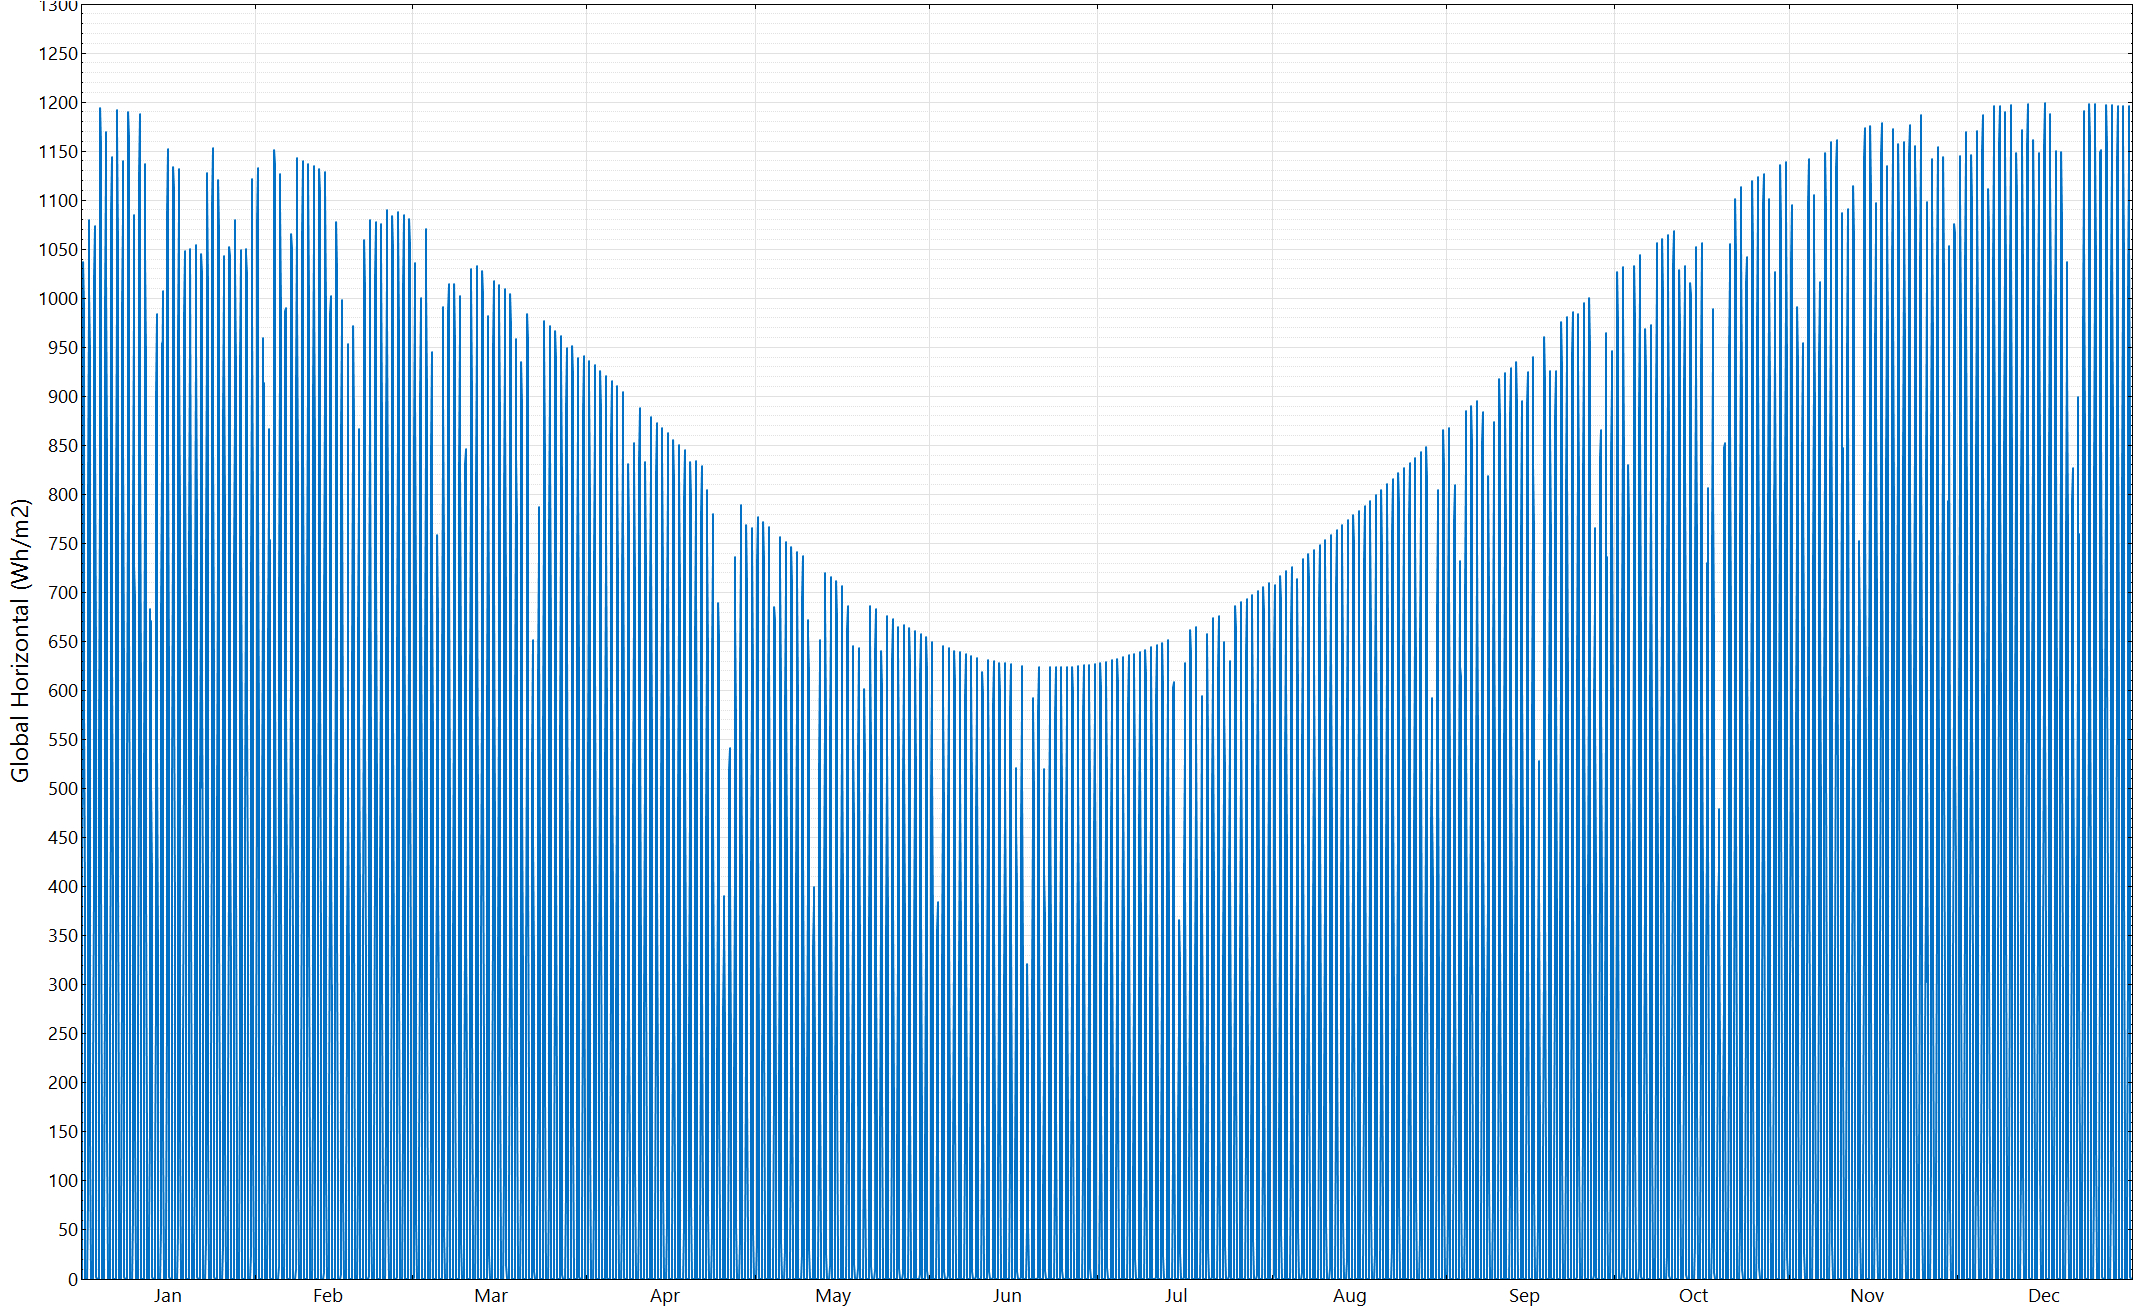
\includegraphics[width=1\textwidth]{FIG/Upington_GHI}
                \caption{Global horizontal}\label{Upington_GHI}
        \end{subfigure}%
\par\medskip % Linebreak      
        \begin{subfigure}[b]{1\textwidth}
                \centering
                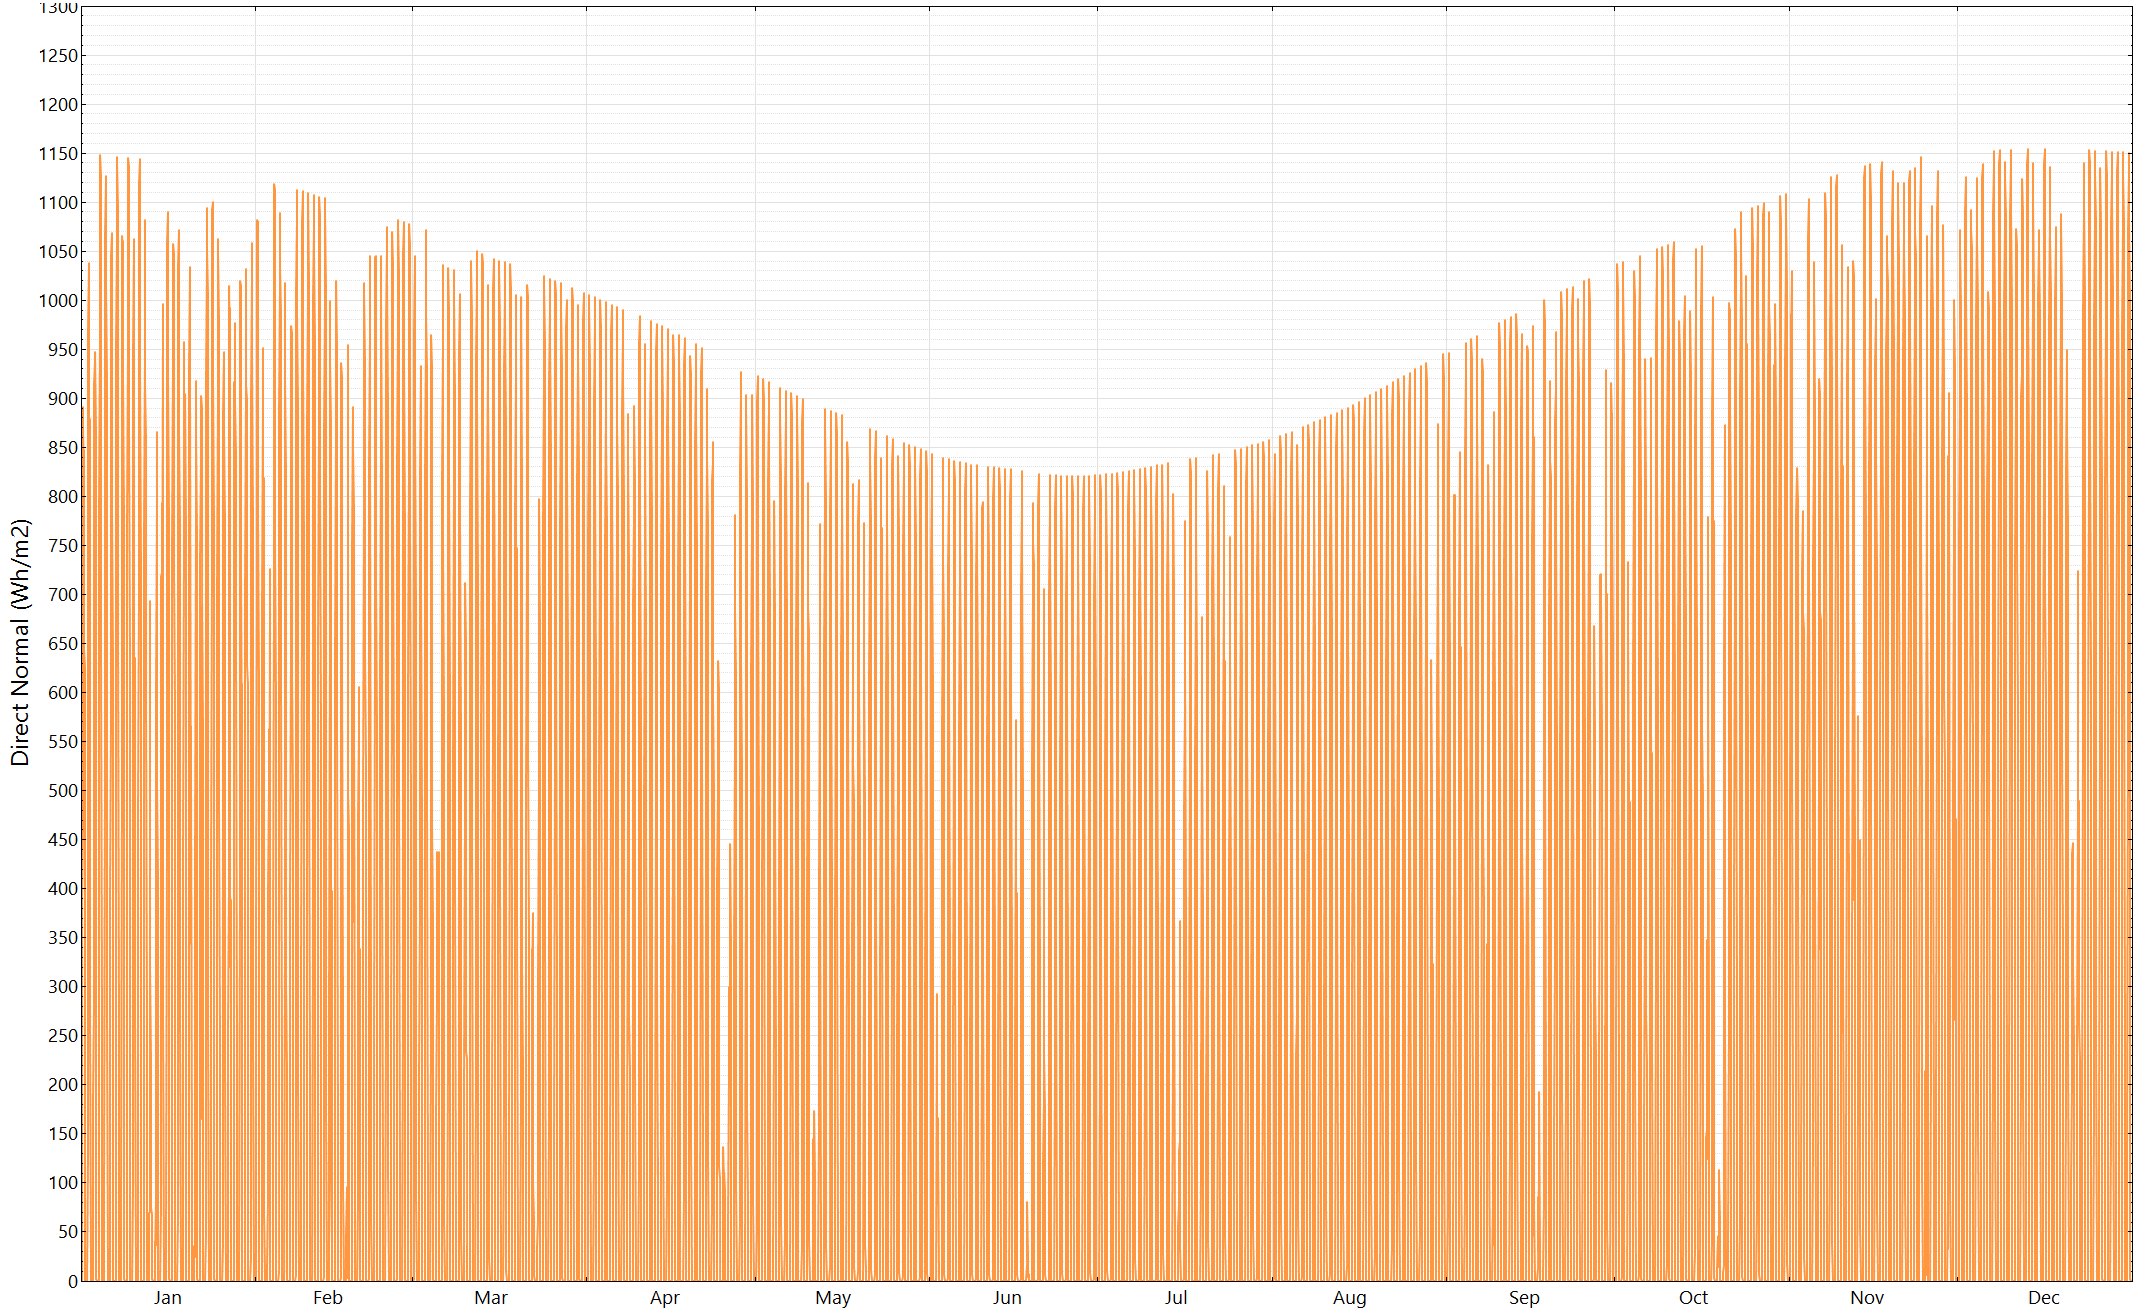
\includegraphics[width=1\textwidth]{FIG/Upington_DNI}
                \caption{Direct normal }\label{Upington_DNI}
        \end{subfigure}%

        \caption[Hourly values of irradiance over a full year from Upington used in the simulation.]{Hourly values of irradiance over a full year from Upington used in the simulation.}\label{Upington_GHI/DNI}
\end{figure}
\newpage \noindent
Most relevant for the simulation is also the position of the sun. SAM calculates the path of the sun by the position of longitude and latitude. Figure~\ref{SunPathUpington} shows the sun path diagram of Upington. From this it appears that the longest day in Upington has 13~h and 56~minutes with a maximum sun height of 85.05$\,^{\circ}$ while the shortest day has just 10~h and 19~minutes and a maximum sun height of 35.93$\,^{\circ}$.
\begin{figure}[htbp]  
\centering
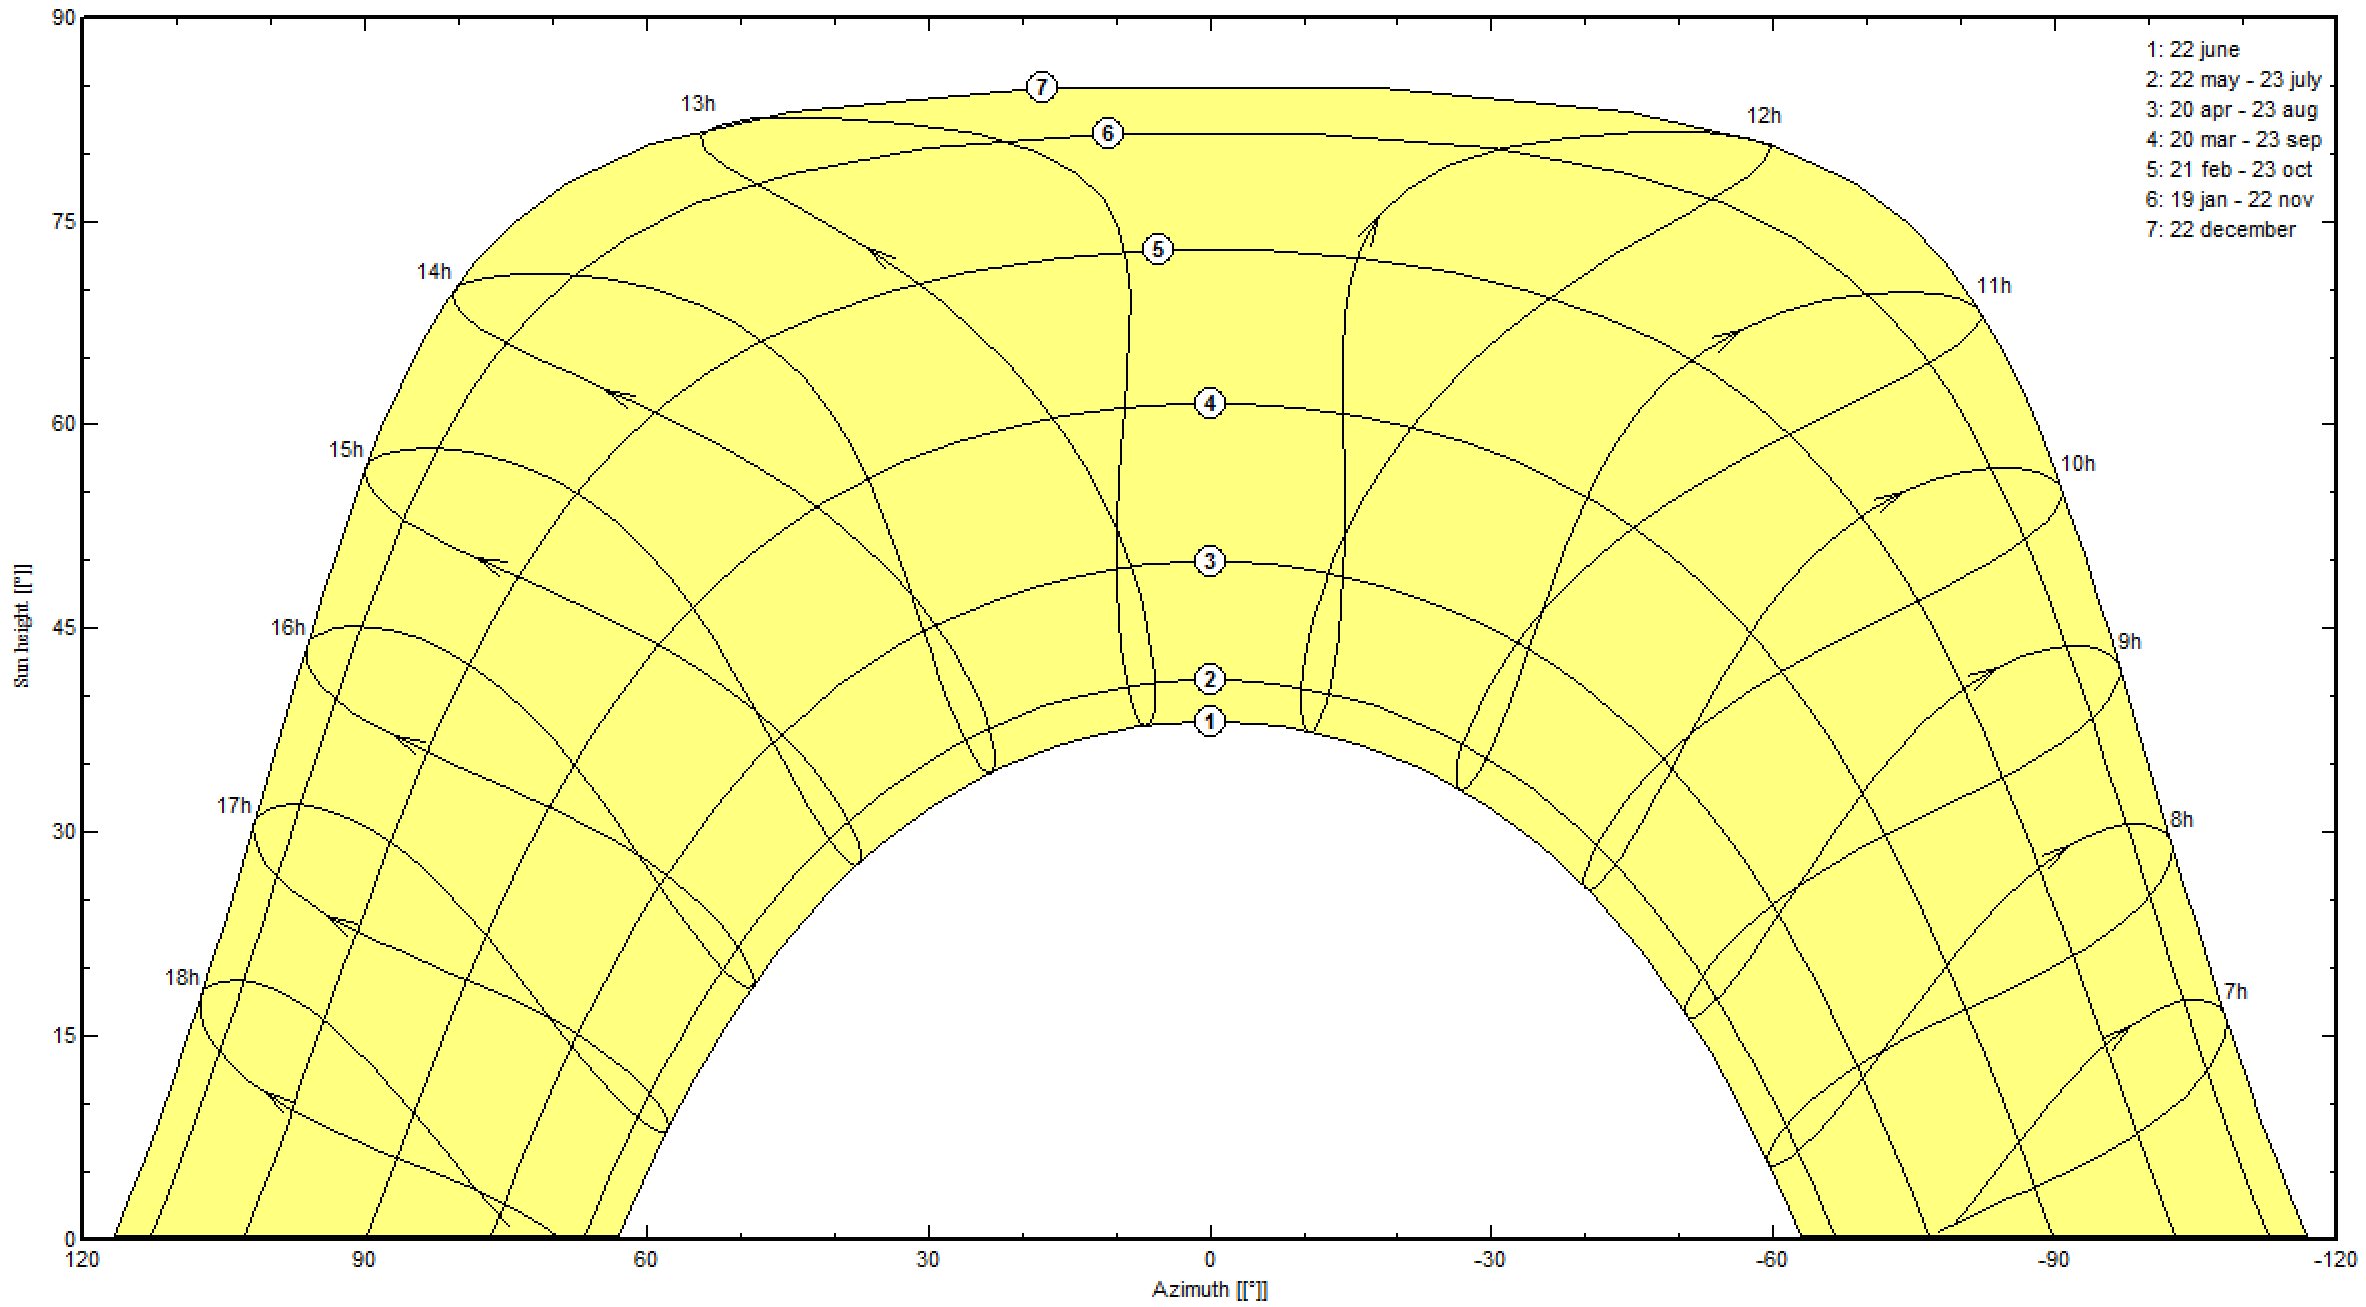
\includegraphics[width=0.95\linewidth]{FIG/SunPathUpington}
\caption[Sun paths diagram Upington.]{Sun paths diagram Upington \cite{PVsystSA2015}.}\label{SunPathUpington}
\end{figure}
\pagebreak 
\section{CR power plant design  and simulation}
For the CR power plant simulation in SAM the “CSP power tower molten salt" model was used. The EPW weather file for Upington from Section~\ref{Location and weather data} was used as an input file to specify the hourly atmospheric conditions. SAM uses the following input data for the simulation:
\begin{itemize}
\item Latitude ($\,^{\circ}$)
\item Longitude ($\,^{\circ}$)
\item Elevation above sea level (m)
\item DNI (W/m\textsuperscript{2})
\item Atmospheric pressure (mbar)
\item Dry bulb temperature ($\,^{\circ}\mathrm{C}$)
\item Wetbulbtemperature($\,^{\circ}\mathrm{C}$)
\item Relative humidity (\%)
\item Wind velocity (m/s)
\end{itemize}
This Chapter describes in detail the crucial inputs of the CR power plant components, namely the  power cycle, heliostat field, tower and receiver and thermal energy storage (TES).\\
As mentioned before are financial parameters and the LCOE calculated separately   Microfoft Excel using a simplified method which is documented in Appendix~\ref{ChapterLCOE} on Page \pageref{ChapterLCOE}. \\
\subsubsection{Simulated configurations}
The simulated configurations had the goal to reach 90~\% of the scheduled production curve by using variation of solar multiple and full load hours of TES. Also the simulated configurations covers a broad view on the technology possibilities. As already mentioned in Section~\ref{Large scale concentrated solar power (CSP) plants} is the SM the ratio of the receivers thermal output to the power cycles thermal input at design point. So a CR system with a SM of 1 has a receiver and a heliostat field which provides the thermal power needed for the power block to run at full load at the system design point. A receiver and collector field with a SM of 1 don't produce enough thermal power to store energy in a TES while feeding the turbine. A CR system with a SM of 1 is just suitable for systems without TES. To covering the scheduled load the solar multiple was varied from 2 to 3.5 in steps of 0.5. Also the storage full load hours were varied from 6 to 16~h in steps of 2~h. The target of 100~MW net capacity was reached with a gross capacity of 111~MW with an estimated gross-to-net conversion factor of 0.90. Table~\ref{tbl: CR_OverallConfig} summarizes the simulated configurations.
\begin{table}[!h]  
  \centering
	\begin{tabular}{ p{4.0cm}  C{1.0cm} C{0.3cm} C{0.3cm} C{0.3cm} C{0.3cm} C{0.3cm} C{0.3cm} |C{0.3cm} C{0.3cm} C{0.3cm} C{0.3cm} C{0.3cm} C{0.3cm} } 
	\hline	
\textbf{Item} & \textbf{Unit} & \multicolumn{12}{c}{\textbf{Value}} \\ \hline \hline
Net turbine capacity & MW\textsubscript{el} & \multicolumn{12}{c}{100} \\
Gross turbine capacity & MW\textsubscript{el} & \multicolumn{12}{c}{111} \\ \hline
Solar multiple & - & \multicolumn{6}{c}{2.0} & \multicolumn{6}{c}{2.5} \\
TES capacity & h &  6 & 8 & 10 & 12 & 14 & 16 &  6 & 8 & 10 & 12 & 14 & 16 \\ \hline 
Solar multiple & - & \multicolumn{6}{c}{3.0} & \multicolumn{6}{c}{3.5} \\
TES capacity & h &  6 & 8 & 10 & 12 & 14 & 16 &  6 & 8 & 10 & 12 & 14 & 16 \\ \hline 
\end{tabular}
\caption[Simulated CR solar multiple and thermal energy storage  configurations.]{Simulated CR solar multiple and thermal energy storage  configurations.}\label{tbl: CR_OverallConfig}
\end{table}
\subsubsection{Power cycle}
The power cycle of the simulated CR system features a Rankine-cycle steam engine, two open feed-water heaters, a pre-heater, boiler and super-heater \cite{NREL2015a}. As mentioned above has the turbine a gross capacity of 111~MW\textsubscript{el} and a nameplate (net) capacity of 100 MW\textsubscript{el}. 
\begin{table}[!h]  
  \centering
	\begin{tabular}{  p{7.0cm}  C{2.0cm}  C{2.0cm} } 
	\hline	
\textbf{Item} & \textbf{Value} & \textbf{Unit} \\ \hline \hline
Turbine design capacity, gross  & 111 & MW\textsubscript{el} \\ 
Turbine design capacity, net & 100 & MW\textsubscript{el} \\ 
Boiler operating pressure & 125 & bar \\ 
Design inlet temperature & 288 & $\,^{\circ}\mathrm{C}$ \\ 
Design outlet temperature & 566 & $\,^{\circ}\mathrm{C}$ \\ 
Cycle conversion efficiency & 41.2 & \% \\ 
Steam generator design thermal power & 269.42 & MW\textsubscript{th} \\
Power block start-up time & 0.5 & h \\ 
Minimum required start-up temperature & 500 & $\,^{\circ}\mathrm{C}$ \\
Plant availability  & 96 & \%\\
Condenser type & air-cooled & - \\ 
\hline
\end{tabular}
\caption[CR power block and condecer input parameter in SAM.]{CR power block and condecer input parameter in SAM.}\label{tbl: CRPowerplant}
\end{table}
The steam generator has a HTF inlet temperature of 566$\,^{\circ}\mathrm{C}$ and outlet temperature of 288$\,^{\circ}\mathrm{C}$ at design point and operates at a pressure of 125 bar. In combination with a air-cooled condenser the CR power cycle system was simulated with a cycle gross efficiency of 41.2\%. A wet-cooled condenser would reaches some higher efficiency, but because of the lack of water in the area of Upington and the requirement by the South African government for CSP plants, a air-cooled condenser was selected. The HTF inlet temperature, pressure and efficiency values where adapted for the configuration from \cite{Kolb2011a}. For starting up the system 
needs 30 minutes and a min. required temperature of 500$\,^{\circ}\mathrm{C}$. A plant availability of 96~\% was adapted from \cite{Morin2012} in order to simulate system down-times for outages or scheduled maintenance.
\subsubsection{Heliostat field}
The heliostat field design was done in SAM using its heliostat field layout optimization tool. For the design, optimization and simulation process, heliostat data from the Sanlúcar 120 heliostat was used \cite{Noone2012}. The Sanlúcar 120 is used in the Planta Solar 10 (PS10) near Seville, Spain and is the origin of Abengoas actual heliostat ASUP 140. For a simulation with the ASUP 140 no sufficient data was available. 
\begin{table}[!htbp]  
  \centering
	\begin{tabular}{ p{4.5cm}  C{1.5cm} C{1.2cm} C{1.2cm} C{1.2cm} C{1.2cm} } 
	\hline	
\textbf{Item} & \textbf{Unit} & \multicolumn{4}{c}{\textbf{Value}} \\ \hline \hline
racking & - &  \multicolumn{4}{c}{two-axis}\\
Height & m  &  \multicolumn{4}{c}{9.45}\\
Width & m  &  \multicolumn{4}{c}{12.84}\\
Reflective area & m\textsuperscript{2} &  \multicolumn{4}{c}{120.00}\\
Heliostat availability& \% &  \multicolumn{4}{c}{99}\\
Design-point DNI & W/m\textsuperscript{2} &  \multicolumn{4}{c}{950}\\
\hline
\textbf{Solar multiple}& \textbf{-} & \textbf{2.0} & \textbf{2.5} & \textbf{3.0} & \textbf{3.5}\\ \hline 
Number of heliostats & - & 9~131 & 11~530 & 13~976 & 16~658 \\
Max. distance from tower & m & 1~528 & 1~708 & 1~883 & 2010 \\
Reflective area  & ha & 109.58 & 138.36 & 167.72 & 199.90 \\
Field land area & ha & 655.59 & 821.92 & 997.95 & 1~190.99\\ 
\hline
\end{tabular}
\caption[CR heliostat parameter.]{CR heliostat parameter.}\label{tbl: CRHeliostats}
\end{table}
The Sanlúcar 120 heliostats have an effective reflective area of 120~m\textsuperscript{2} and are tracked on 2 axes. The heliostat field layout optimization and there design depends on the turbine gross and the SM. The heliostat field was optimized therefore for all four considered configurations. SAM first generates a coarse layout and optimizes the number of heliostats and their position. The goal of the optimization is the maximum flux with minimum power constraints according to the specified design-point DNI which represents the DNI at which the power plant achieves its rated thermal capacity. Table~\ref{tbl: CRHeliostats} summarizes the heliostat datas and the values of the optimized field design for all considered solar multiples.\\
\\
The optimized heliostat field layouts of the four considered SM are depict in Figure~\ref{SM}. In order to avoid mutual shading from the heliostats the heliostat density decreases with distance from the tower. The maximum heliostat distance to the tower rises with the higher SM which can be seen in the field diameter. 
\begin{figure}[!htbp]
        \centering   
        \begin{subfigure}[b]{0.5\textwidth}
                \centering
                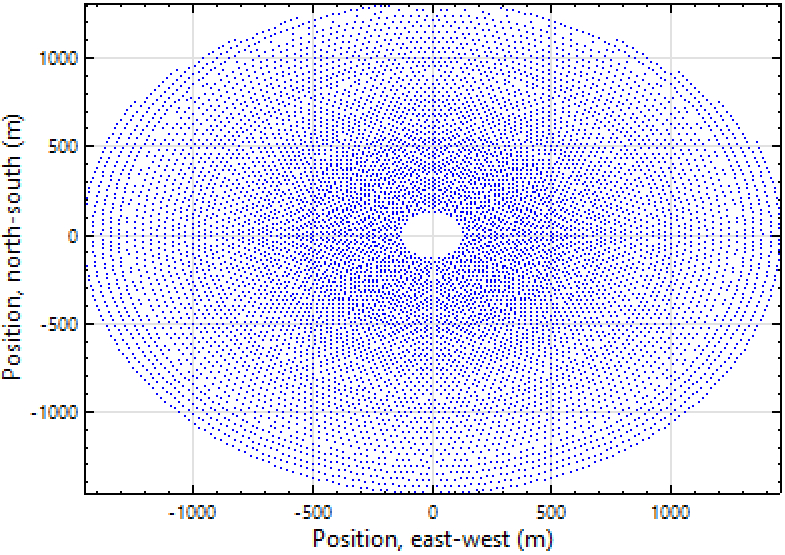
\includegraphics[width=0.95\textwidth]{FIG/SM20}
                \caption{SM~=~2.0}\label{SM2.0}
        \end{subfigure}%
        ~
        \begin{subfigure}[b]{0.5\textwidth}
                \centering
                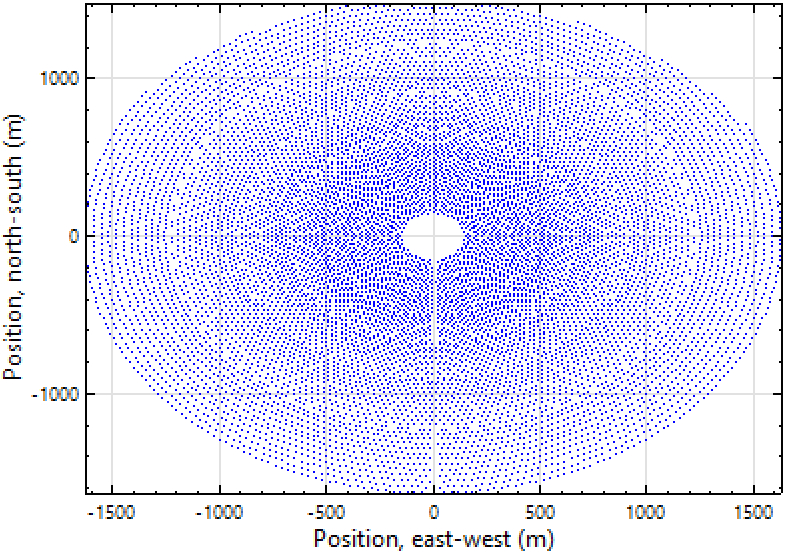
\includegraphics[width=0.95\textwidth]{FIG/SM25}
                \caption{SM~=~2.5}\label{SM2.5}
        \end{subfigure}
        
\par\medskip % Linebreak
                
        \begin{subfigure}[b]{0.5\textwidth}
                \centering
                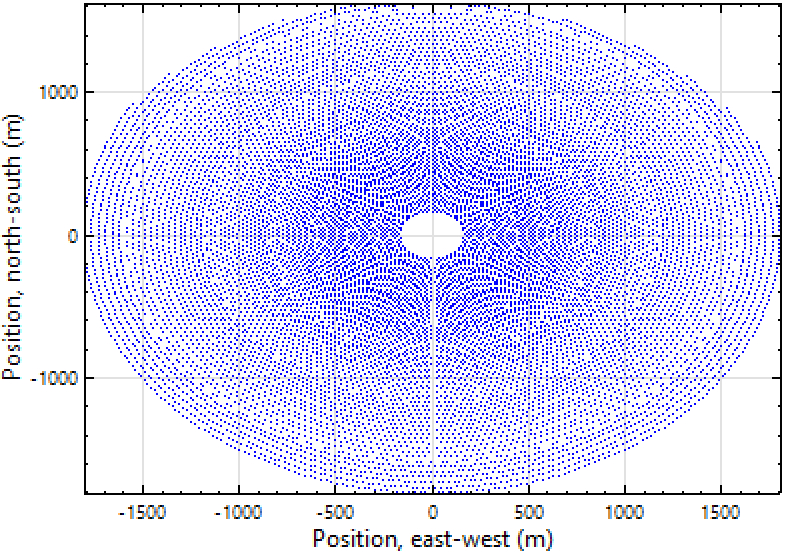
\includegraphics[width=0.95\textwidth]{FIG/SM30}
                \caption{SM~=~3.0}\label{SM3.0}
        \end{subfigure}%
        ~
        \begin{subfigure}[b]{0.5\textwidth}
                \centering
                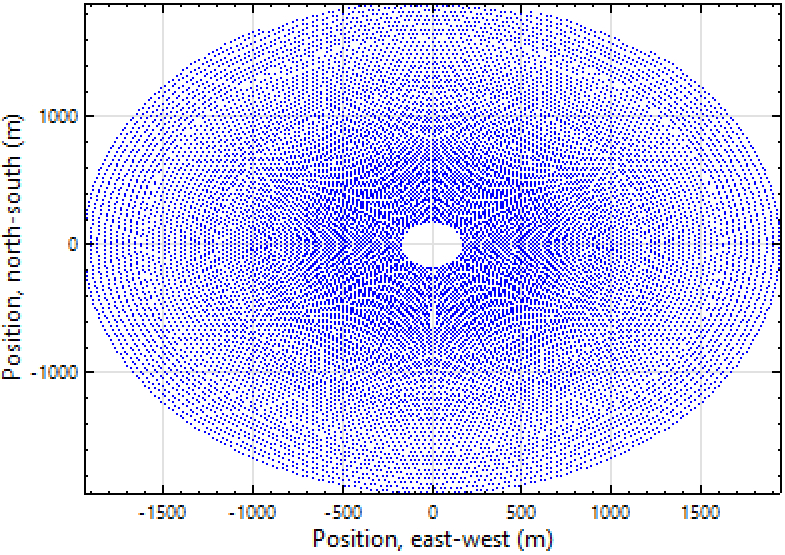
\includegraphics[width=0.95\textwidth]{FIG/SM35}
                \caption{SM~=~3.5}\label{SM3.5}
        \end{subfigure}
        \caption[Simulated heliostat field layout at diferent solar multiples (SM).]{Simulated heliostat field layout at diferent solar multiples (SM).}\label{SM}
\end{figure}
\subsubsection{Tower and receiver}
The receiver collects the concentrated irradiance from the surrounding heliostat field. The simulated receiver is build as an external cylindrical receiver and is configurated with 24 panels of thin walled (1.25 mm) receiver tubes with an outer diameter of 60 mm arranged in a circle around the tower. The receiver tubes are made from 316H stainless steel and the external surfaces of the tubes are coated with a black Pyromark paint. The paint is resistant to high temperatures and thermal cycling, and absorbed 95\% of the incident sunlight. This configuration is similar to the receiver of the  Solar Two Project accept of the outer diameter \cite{Bradshaw2002}. The panels containing molten salt (60~\% NaNO\textsubscript{3} and 40~\% KNO\textsubscript{3}) as heat transfer fluid (HTF). The receiver design inlet temperature of 288$\,^{\circ}\mathrm{C}$ and the outlet temperature of 566$\,^{\circ}\mathrm{C}$ was set before in the power block configuration. In order to achieve the desired receiver thermal power output, the height of the tower and receiver dimensions got also adjust with the optimization of the heliostat field design. The results of the optimization is shown in Table~\ref{tbl: CRSolarfield}, as well as the fixed tower and receiver parameter. The heights of the tower range from 179.77 to 236.50~m. The receiver proportions rises with the SM and the field sizes and results in a receiver thermal power range from 538.8 to 943.0 MW\textsubscript{th}.
\begin{table}[!h]  
  \centering
	\begin{tabular}{ p{5.5cm}  C{1.5cm} C{1.2cm} C{1.4cm} C{1.4cm} C{1.4cm} } 
	\hline	
\textbf{Item} & \textbf{Unit} & \multicolumn{4}{c}{\textbf{Value}} \\ \hline \hline
Receiver configuration & - &  \multicolumn{4}{c}{external cylindrical receiver}\\
Heat transfer fluid & - &  \multicolumn{4}{c}{60~\% NaNO\textsubscript{3} and 40~\% KNO\textsubscript{3}}\\
Inlet temperatures & $\,^{\circ}\mathrm{C}$  &  \multicolumn{4}{c}{288}\\
Outlet temperatures & $\,^{\circ}\mathrm{C}$  &  \multicolumn{4}{c}{566}\\
Receiver tube material & - &  \multicolumn{4}{c}{AISI316 stainless steal}\\
Receiver tube outer diameter & mm &  \multicolumn{4}{c}{60}\\
Receiver tube wall thickness & mm &  \multicolumn{4}{c}{1.25}\\
Number of panels & - &  \multicolumn{4}{c}{24}\\
Absorption factor  & - &  \multicolumn{4}{c}{0.95}\\
\hline
\textbf{Solar multiple} &  & \textbf{2.0} & \textbf{2.5} & \textbf{3.0} & \textbf{3.5}\\ \hline 
Tower height & m & 179.77 & 200.96 & 221.57 &  236.50\\
Receiver height  & m & 22.55 & 25.45 & 27.74 &  29.94\\
Receiver diameter & m & 14.85 & 16.66 & 17.91 & 18.77\\ 
Receiver aperture area & m\textsuperscript{2} & 1~052 & 1~332 & 1~561 & 1~765 \\ 
Receiver thermal power & MW\textsubscript{th} & 538.8 & 673.5 & 808.3 & 943.0 \\
\hline
\end{tabular}
\caption[CR heliostat field parameter.]{CR heliostat field parameter.}\label{tbl: CRSolarfield}
\end{table}
\subsubsection{Thermal energy storage (TES)}
The CR system was simulated using a direct two-tank molten salt thermal energy storage (TES). The storage uses directly the HTF (60~\% NaNO\textsubscript{3} and 40~\% KNO\textsubscript{3}) from the receiver as storage medium. Figure~\ref{towerdirecttwotank} on Page~\pageref{towerdirecttwotank} shows a schema of the direct storage for CR system. The design temperature of the hot storage tank (566$\,^{\circ}\mathrm{C}$) and the cold storage tank (288$\,^{\circ}\mathrm{C}$) depends also from the set value in the power block settings as before the design receiver temperatures. So the design temperature difference between the tanks is 278$\,^{\circ}\mathrm{C}$.\\
\\
As defined at the begining of this Chapter, the full load hours of TES are varied in steps of 2~h from 6 to 16~h. The TES full load hours represents the time in which the storage can supply enough energy to the steam turbine and the power block to run at full design capacity. So a higher value of TES full load hours extended the time that the power plant can run during nights or cloudy days. Table~\ref{tbl: CRTES} shows that with higher TES full load hours the thermal capacity and tank volume increases as well. The simulated storage capacity is in a range of 1~617~MWh\textsubscript{th} using 6 full load hours and 4~311~MWh\textsubscript{th} using 16 full load hours. 
\begin{table}[!h]  
  \centering
	\begin{tabular}{ p{3.9cm}  C{1.0cm} C{1.2cm} C{1.2cm} C{1.2cm} C{1.2cm} C{1.2cm} C{1.2cm} } 
	\hline	
\textbf{Item} & \textbf{Unit} & \multicolumn{6}{c}{\textbf{Value}} \\ \hline \hline
Storage type & - &  \multicolumn{6}{c}{direct two-tank molten salt}\\
Storage fluid & - &  \multicolumn{6}{c}{60~\% NaNO\textsubscript{3} and 40~\% KNO\textsubscript{3}}\\
Hot tank design temp. & $\,^{\circ}\mathrm{C}$ & \multicolumn{6}{c}{566}\\
Cold tank design temp. & $\,^{\circ}\mathrm{C}$ & \multicolumn{6}{c}{288}\\
\hline
\textbf{TES full load hours} & \textbf{h} & \textbf{6} & \textbf{8} & \textbf{10} & \textbf{12} & \textbf{14} & \textbf{16}\\ \hline 
Thermal capacity & MWh\textsubscript{th} & 1~617 & 2~155 & 2~694 & 3~233 & 3~772 &  4~311\\
Storage volume  & m\textsuperscript{3} & 7~757 & 10~229 & 12~787 & 15~345 & 17~902 & 20~460\\
\hline
\end{tabular}
\caption[CR system TES parameter.]{CR system TES parameter.}\label{tbl: CRTES}
\end{table}
\\
SAM 2015.6.30 r3 don't have a power control to follow prescribed hourly net output values. The turbine output of each day needs to be scheduled in front for the simulation. Thereby the parasitic consumer needs highly attention. Figure~\ref{CR_turbineoutput} shows the for the simulation scheduled turbine output matrix. The individual values was fixed during experimental trial. It can be seen that the turbine output is reduced to 50\% during the night as it is specified in the scenario. The power plant follows the schedule till there is no solar irradiance and no more thermal capacity in the storage left to generate power. 
\begin{figure}[htbp]  
\centering
\includegraphics[width=0.95\linewidth]{FIG/CR_turbineoutput}
\caption[TES dispatch control matrix for turbine output fraction of CR simulation in SAM.]{TES dispatch control matrix for turbine output fraction of CR simulation in SAM.}\label{CR_turbineoutput}
\end{figure}
\pagebreak
\subsubsection{Financial parameter}
The financial parameter for the LCOE calculation of the CR power plant are seperated in different specific cost parts and are sumerized in Table~\ref{tbl: CRFinance}. The method for calculating the LCOE is documented in Appendix~\ref{ChapterLCOE} on Page \pageref{ChapterLCOE} using a lifetime of 25~years and a real interest rate of 7.5~\% \cite{FraunhoferISE2013}. The interest rate could be reduced with a rising market potential.\\
\\
The specific costs of the heliostat field of 180\$/m\textsuperscript{2} coming from J. B. Blackmon \cite{Blackmon2012}. He analyzed the costs of heliostat as a function of area for a representative solar central receiver power plant and calculated the total installed costs for a field of 5~000 heliostats with 148~m\textsuperscript{2} reflective area of approximately 180~\$/m\textsuperscript{2}. The analyze results showed that the costs are increasing with the size of the heliostats from 40~m\textsuperscript{2} on. So the adopted value of 180~\$/m\textsuperscript{2} reflective area for 140~m\textsuperscript{2} heliostats can be assumed as conservative.\\
The remaining investment costs are based on the "Power Tower Technology Roadmap and Cost Reduction Plan" \cite{Kolb2011} from 2011.\\
On top of the investment costs a came 15 \% once-off surcharge for EPC and contingencies \cite{Platzer2014}.\\
Fichtner analyzed the annual O\&M costs with 1.84-1.96~\% of the total investment costs for CR power plants in SA \cite{Fichtner2010}. The value of 2~\% can so also be assumed as conservative.\\
The costs for the land purchase comes from the "African Agriculture Review" report of the Nedbank Capital, which reported the prices for farmland in SA. For the LCOE calculation of the CSP and PV system was the land purchase costs of \$3,000/ha assumed which is based on these report \cite{Cassell2012}.

\begin{table}[!h]  
  \centering
	\begin{tabular}{  p{5.0cm} C{2.0cm} C{1.5cm}  C{1.5cm}  C{4.0cm} } 
	\hline	
\textbf{Item} & \textbf{Symbol}& \textbf{Value} & \textbf{Unit} & \textbf{Source}\\ \hline \hline

Heliostat field &$c_{HF}$ & 180 & \$/m\textsuperscript{2} & \cite{Blackmon2012}\\ 
Power block & $c_{PB,CR}$ & 1000 & \$/kW\textsubscript{el} & \cite{Kolb2011}\\ 
Thermal energy storage&$c_{TES,CR}$ & 30 & \$/kWh\textsubscript{th}  & \cite{Kolb2011}\\ 
Tower and receiver& $c_{T+R}$& 200 & \$/kW\textsubscript{th}  & \cite{Kolb2011}\\ 
Annual O\&M & $f_{O\&M,CR}$ & 2 & \% &\cite{Fichtner2010}\\
Land purchase&$c_{LP}$ & 3~000 & \$/ha & \cite{Cassell2012}\\ \hline
Lifetime &$n$ & 25 & years & \cite{FraunhoferISE2013} \\ 
Interest rate & $i_{CR}$ & 7.5 & \% & \cite{FraunhoferISE2013} \\ 
Surcharge for EPC, project management and risk & $f_{EPC,CR}$& 15 & \% & \cite{Platzer2014} \\
Total plant availability & $f_{avail,plant,CR}$ & 96 & \% & \cite{Morin2012} \\ 
\hline
\end{tabular}
\caption[Finacial input parameter for CR-simulation in SAM.]{Finacial input parameter for CR-simulation in SAM.}\label{tbl: CRFinance}
\end{table}
\pagebreak
\section{PTC power plant design  and simulation}
The PTC power plant was simulation in the “CSP parabolic trough (physical)" model in SAM using the option "no financial model". As before the input the EPW weather file to specify the hourly atmospheric conditions from Section~\ref{Location and weather data} was used. For the PTC simulation SAM uses the following input data:
\begin{itemize}
\item Latitude ($\,^{\circ}$)
\item Longitude ($\,^{\circ}$)
\item Elevation above sea level (m)
\item DNI (W/m\textsuperscript{2})
\item Atmospheric pressure (mbar)
\item Dry bulb temperature ($\,^{\circ}\mathrm{C}$)
\item Wetbulbtemperature($\,^{\circ}\mathrm{C}$)
\item Relative humidity (\%)
\item Wind velocity (m/s)
\end{itemize}
This Chapter describes in detail the input data of the PTC power plant simulation by there components, namely the  power cycle, solar collector, solar receiver, solar field and thermal energy storage (TES).\\
Also for the simulation of the PTC are the financial parameters and the LCOE calculated separately Microfoft Excel using a simplified method which is documented in Appendix~\ref{ChapterLCOE} on Page \pageref{ChapterLCOE}.
\subsubsection{Simulated configurations}
In order to reaching the goal of covering 90 \% of the scheduled production curve also the simulated PTC power plant used a variation of solar multiple and full load hours of TES. To covering the scheduled load the solar multiple was varied from 2 to 5.0 in steps of 5.0. This is significantly higher SM compared the simulated CR system was necessary to reach the 90 \% covering factor. As before with the simulation of the CR, the storage full load hours were varied from 6 to 16 h in steps of 2 h. The target of 100 MW net capacity was reached with a gross capacity of 120 MW with an estimated gross-to-net conversion factor of 0.83. The comparatively high gross turbine output is nessasary for the high parasitic burden of the system. Table~\ref{tbl: PTC_OverallConfig} summarizes the simulated configurations.
\begin{table}[!h]  
  \centering
	\begin{tabular}{ p{4.0cm}  C{1.0cm} C{0.3cm} C{0.3cm} C{0.3cm} C{0.3cm} C{0.3cm} C{0.3cm} |C{0.3cm} C{0.3cm} C{0.3cm} C{0.3cm} C{0.3cm} C{0.3cm} } 
	\hline	
\textbf{Item} & \textbf{Unit} & \multicolumn{12}{c}{\textbf{Value}} \\ \hline \hline
Net turbine capacity & MW\textsubscript{el} & \multicolumn{12}{c}{100} \\
Gross turbine capacity & MW\textsubscript{el} & \multicolumn{12}{c}{120} \\ \hline
Solar multiple & - & \multicolumn{6}{c}{2.0} & \multicolumn{6}{c}{2.5} \\
TES capacity & h &  6 & 8 & 10 & 12 & 14 & 16 &  6 & 8 & 10 & 12 & 14 & 16 \\ \hline 
Solar multiple & - & \multicolumn{6}{c}{3.0} & \multicolumn{6}{c}{3.5} \\
TES capacity& h &  6 & 8 & 10 & 12 & 14 & 16 &  6 & 8 & 10 & 12 & 14 & 16 \\ \hline 
Solar multiple & - & \multicolumn{6}{c}{4.0} & \multicolumn{6}{c}{4.5} \\
TES capacity& h &  6 & 8 & 10 & 12 & 14 & 16 &  6 & 8 & 10 & 12 & 14 & 16 \\ \hline 
Solar multiple & - & \multicolumn{6}{c}{5.0} & \multicolumn{6}{c}{ } \\
TES capacity& h &  6 & 8 & 10 & 12 & 14 & 16 &  \multicolumn{6}{c}{ } \\ \hline 
\end{tabular}
\caption[Simulated PTC solar multiple and thermal energy storage  configurations.]{Simulated PTC solar multiple and thermal energy storage  configurations.}\label{tbl: PTC_OverallConfig}
\end{table}

\subsubsection{Power cycle}
The PTC system also uses the steam Rankine cycle technology. In the modeled cycle, feedwater is heated in open (mixed stream) feedwater heaters with two intermediate turbine extractions - once for high pressure and once for low pressure, and the steam generation equipment consists of a preheater, boiler, and superheater. The HTF temperature at the field outlet is bound primarily by HTF stability, so maximum HTF temperatures for oil troughs typically range between 370$\,^{\circ}\mathrm{C}$ and 410$\,^{\circ}\mathrm{C}$. The turbine has a gross capacity of 120~MW\textsubscript{el}. So the net turbine capacity output at design (nameplate) is 100~MW\textsubscript{el}. The design inlet temperature of the HTF in the steam generator is 393$\,^{\circ}\mathrm{C}$ and outlet temperature of 293$\,^{\circ}\mathrm{C}$ at design point and operates at a pressure of 100 bar.\\
\\
Table~\ref{tbl: PTCPowerplant} shows the input parameter for the power block design in SAM. Besides the capacity of the turbine and the condecer type, the parameters are coming from \cite{Wagner2011}. It is obviously, that the cycle conversion efficiency of the PTC power plant is lower than that one from the CR power plant. This is trace back to the lower cycle temperatures and the thereby resulting lower steam pressure in the turbine.\\
\\
The air-cooled condenser was selected here as well, because water is an valuable resource in the region of Upington. The cooling system is designed to covers the stem generator thermal power. 
\begin{table}[!h]  
  \centering
	\begin{tabular}{  p{7.0cm}  C{2.0cm}  C{2.0cm} } 
	\hline	
\textbf{Item} & \textbf{Value} & \textbf{Unit} \\ \hline \hline
Turbine design capacity, gross  & 110 & MW\textsubscript{el} \\ 
Turbine design capacity, net & 100 & MW\textsubscript{el} \\ 
Boiler operating pressure & 100 & bar \\ 
Design inlet temperature & 393 & $\,^{\circ}\mathrm{C}$ \\ 
Design outlet temperature & 291 & $\,^{\circ}\mathrm{C}$ \\ 
Cycle conversion efficiency & 37.74 & \% \\ 
Steam generator design thermal power & 318.0 & MW\textsubscript{th}  \\
Power block start-up time & 0.5 & h \\ 
Minimum required start-up temperature & 300 & $\,^{\circ}\mathrm{C}$ \\
Maximum turbine over design operation & 90 & \%\\
Condenser type & air-cooled & - \\ 
\hline
\end{tabular}
\caption[PTC power block and condecer input parameter in SAM.]{PTC power block and condecer input parameter in SAM.}\label{tbl: PTCPowerplant}
\end{table}
\subsubsection{Solar collector (SCA)}
For the simulation of the PTC system the Ultimate Trough was selected as solar collector assembly (SCA). This collector is currently not in commercial use, but comparable troughs with similar characteristics are under construction. So the Ultimate Trough can be adopted  without technical modifications and no increase of risk. Figure~\ref{PTC_Ultimate_config} shows the information of the technical input parameter for SAM. These coming directly from a publication of the developer of the Ultimate Trough, Flabeg GmbH and sbp sonne GmbH \cite{Riffelmann2014}. 
\begin{figure}[bhtp]
\centering
\includegraphics[width=0.95\linewidth]{FIG/PTC_Ultimate_config}
\caption[Screenshot of Ultimate Trough input parameter for SAM.]{Screenshot of Ultimate Trough input parameter for SAM.}\label{PTC_Ultimate_config}
\end{figure}
The section "Optical Calculation" shows, that the total optical efficiency at design of the Ultimate Trough is 89.9~\%. The dimensions and main characteristics of the HCE is shown in the section "Receiver Geometry".
\subsubsection{Solar receiver (HCE)}
As heat collecting element (HCE) Schott's PTR80 was selected. This receiver tube has with 0.08~m an extended tube outer diameter. Thereby the tube can contain more HTF and reduce the mass flow in the tubes. Figure~\ref{PTC_HCE} shows the for the simulation inserted parameter. The values are the results of measurements of outdoor optical efficiency and indoor receiver heat loss of parabolic trough collector from researchers of National Renewable Energy Laboratory \cite{Kutscher2012}.
\begin{figure}[htbp]  
\centering
\includegraphics[width=0.95\linewidth]{FIG/PTC_HCE}
\caption[Screenshot of Schott PTR80 input parameter for SAM.]{Screenshot of Schott PTR80 input parameter for SAM.}\label{PTC_HCE}
\end{figure}
The section "Parameter and Variations" shows the different conditions of the HCE. Variation 1 shows the optimal condition of the HCE with annulus pressure of 0.0001 torr (0.000133~hPa), so an vacuum. The estimated average heat lost is 190~W/m. This Variation counts for 98.5~\% of all HCEs. In Variation 2 the vacuum is lost and which strongly affects the heat loss. It is 1~270~W/m and counts for 1~\% of all HCEs. In Variation 3 also the protection glass is broken, so the heat loss increase to 1~500~W/m. The total weighted losses is 207.35~W/m heat loss at design and about 0.85 optical derate and is shown at the last section most below.
\subsubsection{Solar field}
PTC solar fields are separated in sections. In the simulation of the PTC system the solar field is designed in two sections. Each section carries a feed pipe and a return pipe to transport the thermal energy to the power block. Attached to the header pipes are many loops, which contains the SCAs, the HCEs and the HTF. Figure~\ref{PTC_Field_ultimate} shows an typical layout for PTC system with two field subsections. As in the Figure is the simulated PTC system designed by four SCAs per loop \cite{Riffelmann2014}.
\begin{figure}[htbp]  
\centering
\includegraphics[width=0.9\linewidth]{FIG/PTC_Field_ultimate}
\caption[Typical configuration of a solar field layout with two field subsections for a Ultimate Trough.]{Typical configuration of a solar field layout with two field subsections for a Ultimate Trough \cite{Riffelmann2014}.}\label{PTC_Field_ultimate}
\end{figure}
\\
As mentioned before synthetic oil is used as HTF for the simulation of the PTC system. The current standard for HTF in PTC systems is Terminol VP-1. The input parameter for the HTF are shown in Figure~\ref{PTC_HTF} and are limited by the performance characteristics of Terminol VP-1 of 12 to 400$\,^{\circ}\mathrm{C}$ \cite{Therminol2015}. The velocity range of Therminol VP-1 should be in the range of 0.36 and 4.97 m/s \cite{Wagner2014} and is affected by the inner tube diameter of the HCE, the HTF density and the loop flow rate \cite{NREL2015a}. A freeze protection temperature for the HTF of 150$\,^{\circ}\mathrm{C}$ is typically and also assumed for the simulation \cite{Kearney2002}.
\begin{figure}[htbp]  
\centering
\includegraphics[width=0.6\linewidth]{FIG/PTC_HTF}
\caption[Screenshot of HTF input parameter for SAM.]{Screenshot of HTF input parameter for SAM.}\label{PTC_HTF}
\end{figure}
\\
The size of the solar field is strongly effected by the solar multiple and the thermal demand of the steam Rankine cycle. At a solar multiple of 1 (design thermal power of the steam generator) the solar field requires 453003~m\textsuperscript{2} ($\approx$45.3~ha) reflective aperture area of SCA. 65.86 ($\approx$66) loops are required at a SM of 1. The number of loops and so also the field size multiplies by the value of the SM.\\
\\
Also the the solar field area and thereby the total land area depending by the SM. Equation~\ref{GL_PTCSolarfieldarea} shows the influence on the solar field area of the ratio between the row spacing and the SCA width. The roe spacing is assumed by 18~m between the parallel SCAs. The total land area results by Equation~\ref{GL_PTCtotallandarea} and is the solar field area multiplies by the factor of non-solar field area. The factor is assumed by 1.4 in the simulation \cite{NREL2015a}.
\begin{align}
\textrm{solar field area }(m^2) =\textrm{aperture area }(m^2) \times \frac{\textrm{row spacing }(m)}{ \textrm{SCA width }(m)} \label{GL_PTCSolarfieldarea}
\end{align}
\begin{align}
\textrm{total land area }(m^2) =\textrm{solar field area }(m^2) \times  \textrm{non-solar field multiplier}\label{GL_PTCtotallandarea}
\end{align}
Table~\ref{tbl: PTCSolarfield} shows the solar field simulation parameter of the PTC system for the simulation configuration values of the solar multiple. The parameters of the Table comes from the above mentioned relations between the Items. The design power of the steam generator (SG) stays at 318.0~MW\textsubscript{th} while the solar field thermal output rises proportional through the SM. 
\begin{table}[!h]  
  \centering
	\begin{tabular}{ p{3.3cm} C{1.1cm} C{1.1cm} C{1.1cm} C{1.1cm} C{1.1cm} C{1.1cm} C{1.1cm} C{1.1cm} } 
	\hline	
\textbf{Item} & \textbf{Unit} & \multicolumn{7}{c}{\textbf{Value}} \\ \hline \hline
SG Design power & MW\textsubscript{th} &  \multicolumn{7}{c}{318.0}\\
Design-point DNI & W/m &  \multicolumn{7}{c}{950}\\
\hline
\textbf{Solar multiple} &  & \textbf{2.0} & \textbf{2.5} & \textbf{3.0} & \textbf{3.5} & \textbf{4.0} & \textbf{4.5} & \textbf{5.0}\\ \hline 
Field th. output & MW\textsubscript{th} & 636 & 795 & 954 & 1~113 & 1~272 & 1~431 & 1~590\\
Number of loops  & - & 132 & 165 & 198 & 231 & 264 & 297 & 330\\ 
Aperture refl. area & ha & 90.6 & 113.3 & 135.9 & 158.6 & 181.2 & 203.9 & 226.5\\ 
Total land area & ha & 675 & 845 & 1013 & 1~182 & 1~351 &1~540 & 1~689\\ 
\hline
\end{tabular}
\caption[PTC solar field parameter.]{PTC solar field parameter.}\label{tbl: PTCSolarfield}
\end{table}
\pagebreak
\subsubsection{Thermal energy storage (TES)}
The thermal energy storage (TES) of the simulated PTC system uses a indirect two-tank molten salt system with "Hitec Solar Salt" as storage fluid. This storage fluid is made from sodium nitrate (60~\% NaNO\textsubscript{3}) and potassium nitrate (40~\% KNO\textsubscript{3}). Solar Salt needs an minimum operating temperature of 238$\,^{\circ}\mathrm{C}$ and and has a maximum operating temperature of 593$\,^{\circ}\mathrm{C}$. \cite{Suite2011,Kearney2003}\\
\begin{table}[!b]  
  \centering
	\begin{tabular}{ p{3.9cm}  C{1.0cm} C{1.2cm} C{1.2cm} C{1.2cm} C{1.2cm} C{1.2cm} C{1.2cm} } 
	\hline	
\textbf{Item} & \textbf{Unit} & \multicolumn{6}{c}{\textbf{Value}} \\ \hline \hline
Storage type & - &  \multicolumn{6}{c}{indirect two-tank molten salt}\\
Storage fluid & - &  \multicolumn{6}{c}{Hitec Solar Salt}\\
Hot tank design temp. & $\,^{\circ}\mathrm{C}$ & \multicolumn{6}{c}{391}\\
Cold tank design temp. & $\,^{\circ}\mathrm{C}$ & \multicolumn{6}{c}{293}\\
\hline
\textbf{TES full load hours} & \textbf{h} & \textbf{6} & \textbf{8} & \textbf{10} & \textbf{12} & \textbf{14} & \textbf{16}\\ \hline 
Thermal capacity & MWh\textsubscript{th} & 1~908 & 2544 & 3~180 & 3~816 & 4~452 & 5~087 \\
Storage volume  & m\textsuperscript{3} & 25~805 & 34~407 & 43008 & 51~610 & 60~212 & 68~813\\
\hline
\end{tabular}
\caption[PTC system TES parameter.]{PTC system TES parameter.}\label{tbl: PTCTES}
\end{table}
\\
The storage design temperatures depends from the solar field design temperatures, so the designed temperature difference is 98~K. As it is shown in Table~\ref{tbl: PTCTES} the operating temperature limits fits with the storage tank design temperatures. The heater set point is 265$\,^{\circ}\mathrm{C}$ for both storage tanks. The TES full load hours goes from 6 to 16 in steps of 2. The thermal capacity and also the storage volume rises with the TES full load hours. The simulated stored thermal capacity reaches from 1~908~MWh\textsubscript{th}  at 6 full load hours up to 5~087~MWh\textsubscript{th} at 6 full load hours. It is obviously, that the storage volume of the PTC needs to be more than 3 times that much than the storage volume of the CR system. This is the result of lower temperature difference of the HTF and the turbine design capacity.\\
\\
Also for the simulation of the PTC system the dispatch control of the turbine output fraction in the storage settings was used. Figure~\ref{PTC_turbineoutput} shows the dispatch control matrix for the turbine output fraction.
\begin{figure}[htbp]  
\centering
\includegraphics[width=0.95\linewidth]{FIG/PTC_turbineoutput}
\caption[TES dispatch control matrix for turbine output fraction of PTC simulation in SAM.]{TES dispatch control matrix for turbine output fraction of PTC simulation in SAM.}\label{PTC_turbineoutput}
\end{figure}
\pagebreak
\subsubsection{Financial parameter}
The financial parameter for calculating the LCOE of the simulated configuration are shown in Table~\ref{tbl: PTCFinance}. As before at the CR is the PTC power plant calculated over a lifetime of 25~years using a real interest rate of 7.5~\% \cite{FraunhoferISE2013}. Also the total plant availability of  15~\% once-off surcharge for EPC and contingencies on the total investment costs are equal to the CR \cite{Platzer2014}.
\\
The specific costs for the collector field inclusive HTF-system is assumed with 275~\$/m\textsuperscript{2} from \cite{Morin2012}. These specific cost could also be reduced by 25~\% by using the assumed cost reduction from Flabeg \cite{FLABEG_FE_GmbH2015}. So the for the simulation assumed costs are highly conservative.\\
The specific costs for the power block are the same as at the CR but from other sources \cite{Platzer2014}. \\
The specific costs of 50~\$/kWh\textsubscript{th} for the TES of the PTC are up to 50\% higher than the CR costs \cite{Platzer2014}. This is reduce to the lower energy density using lower storage temperatures \cite{Steinmann2015}. Other expected specific costs between 35 and 50~\$/kWh\textsubscript{th}  \cite{Steinmann2012}.\\
As before Fichtner analyzed also the annual O\&M costs for PTC power plants in SA and results costs of 1.96-1.97~\% of the total investment costs \cite{Fichtner2010}. The value of 2~\% can so also be assumed as conservative.\\
The costs for the land purchase comes from the "African Agriculture Review" report of the Nedbank Capital, which reported the prices for farmland in SA. For the LCOE calculation of the CSP and PV system was the land purchase costs of \$3,000/ha assumed which is based on these report \cite{Cassell2012}.
\begin{table}[!h]  
  \centering
	\begin{tabular}{  p{5.0cm} C{2.0cm} C{1.5cm}  C{1.5cm}  C{4.0cm} } 
	\hline	
\textbf{Item} & \textbf{Symbol}& \textbf{Value} & \textbf{Unit} & \textbf{Source}\\ \hline \hline

Collector field/HTF-system & $c_{CF}$ & 275 & \$/m\textsuperscript{2} & \cite{Morin2012}\\ 
Power block &$c_{PB,PTC}$ & 1000 & \$/kW\textsubscript{el} & \cite{Platzer2014}\\ 
Thermal energy storage & $c_{TES,PTC}$ & 50 & \$/kWh\textsubscript{th} & \cite{Platzer2014}\\ 
Land purchase & $c_{LP}$ & 3~000 & \$/ha & \cite{Cassell2012} \\ 
Annual O\&M & $f_{O\&M,PTC}$ &2&\% &\cite{Fichtner2010}\\ 
\hline
Lifetime&$n$ & 25 & years & \cite{FraunhoferISE2013} \\ 
Interest rate& $i_{PTC}$& 7.5 & \% & \cite{FraunhoferISE2013} \\ 
Surcharge for EPC, project management and risk & $f_{EPC,PTC}$ & 15 & \% & \cite{Platzer2014} \\
Total plant availability &$f_{avail,plant,PTC}$ & 96 & \% & \cite{Morin2012} \\ 
\hline
\end{tabular}
\caption[Finacial input parameter for PTC-simulation in SAM.]{Finacial input parameter for PTC-simulation in SAM.}\label{tbl: PTCFinance}
\end{table}
\pagebreak
\section{PV power plant with electrical energy storage design and simulation}
For this simulation a PV power plant was extended with an electrical energy storage (EES). This extended PV power plant was simulated in SAM's "Photovoltaic (detailed)" model with enabled battery storage option. Also for this simulation was the EPW weather file for Upington from Section~\ref{Location and weather data} used. For the PV simulation SAM uses the following input data:
\begin{itemize}
\item Latitude ($\,^{\circ}$)
\item Longitude ($\,^{\circ}$)
\item Elevation above sea level (m)
\item GHI, DNI and DHI (W/m\textsuperscript{2})
\item Dry bulb temperature ($\,^{\circ}\mathrm{C}$)
\item Wind velocity (m/s)
\end{itemize}
This section describes in detail the residual input data of the PV power plant with adapted battery storage. As before in the sections of simulated CSP technologies first the essential components of the system are defined. The financial parameters and the LCOE for this simulation was also here calculated separately and is documented in Appendix~\ref{ChapterLCOE} on Page \pageref{ChapterLCOE}.\\
\\
As mentioned at the beginning of these Chapter this must be seen as theoretical simulation. Actually there are not that large electrical energy storage systems in form of battery storage available.\\
\\
For this simulation the load was conected to the PV and Battery system as shown on Figure~\ref{PV_model_config}. The load shape was defined as before specified before in Chapter~\ref{Overall simulated configuration} and simulates the demand of the power grid. As it is shown there is also the actual power grid connected as additional component, but for this simulation just the power flows between PV, battery and load is in focus. As it is shown in the Figure, SAM actually just support the battery connection at the AC-bus via a power conversion system and is not able to simulate direct DC-connected batteries besides the PV-array before the PV-inverter. However in order to produce comparable results SAM was also used for the simulation of the PV power plant. As mentioned before this system contains out of the PV system with solar modules, solar and inverter and are described in the following section as well as the electrical energy storage.
\begin{figure}[htbp]  
\centering
\includegraphics[width=0.55\linewidth]{FIG/PV_model_config}
\caption[Model of the configurated PV plus batterie scheme.]{Model of the configurated PV plus batterie scheme \cite{Diorio2015}.}\label{PV_model_config}
\end{figure}
\subsubsection{Simulated configurations}
The configurations of the PV system with adapted electrical energy storage has also the target to reach 90~\% of the scheduled production curve from Section~\ref{Overall simulated configuration}. To reach this target it is necessary to over scale the energy production of the PV system to produce enough power to covers the given load and load the storage during the day. This is quite similar to the solar multiple of the CSP system, but can not be put on a same level. Therefore this over scaling will be called "PV multiple" (PVM) and means the multiple of the PV inverter output. For example the system with a maximum inverter output of 100~MW\textsubscript{el} is a PVM of 1 than has the PV system with a PVM of 2 a maximum inverter output of 200~MW\textsubscript{el}. 
\begin{table}[!b]  
  \centering
	\begin{tabular}{ p{4.0cm}  C{1.0cm} C{0.3cm} C{0.3cm} C{0.3cm} C{0.3cm} C{0.3cm}  | C{0.3cm} C{0.3cm} C{0.3cm} C{0.3cm} C{0.3cm} } 
	\hline	
\textbf{Item} & \textbf{Unit} & \multicolumn{10}{c}{\textbf{Value}} \\ \hline \hline
Maximum load supply & MW\textsubscript{el} & \multicolumn{10}{c}{100} \\ \hline
PV multiple & - & \multicolumn{5}{c}{1.0} & \multicolumn{5}{c}{1.8} \\
EES capacity & h & \multicolumn{5}{c}{-} & 4 & 5 & 6 & 7 & 8 \\ \hline 
PV multiple & - & \multicolumn{5}{c}{2.0} & \multicolumn{5}{c}{2.2} \\
EES capacity& h &  4 & 5 & 6 & 7 & 8 & 4 & 5 & 6 & 7 & 8 \\ \hline 
PV multiple & - & \multicolumn{5}{c}{2.4} & \multicolumn{5}{c}{2.6} \\
EES capacity & h & 4 & 5 & 6 & 7 & 8 & 4 & 5 & 6 & 7 & 8 \\ \hline 
\end{tabular}
\caption[Simulated configurations of the PV system with adapted EES.]{Simulated configurations of the PV system with adapted EES.}\label{tbl: PV_OverallConfig}
\end{table}
The simulated system load is maximum 100~MW\textsubscript{el}, so this is also the maximum supply of the system. The PV system was simulated one time without storage and a maximum inverter output of 100~MW\textsubscript{el} which is a PVM of 1. After that, the system was simulated in steps 0.2 of the PVM from 1.8 to 2.6. The adapted energy storage capacity was simulated from 4 to 8 hours in hourly steps. This storage capacity range is also defined for large-scale off-grid application in \cite{IEA2014c}. Table~\ref{tbl: PV_OverallConfig} summarizes the simulated configurations.
\subsubsection{PV system}
The simulated PV system is orientated at actual PV systems in SA. Therefore the currently under construction situated Mulilo Sonnedix Prieska PV Project in the Northern Cape will serve as a role model for the main components. In this 75~MW\textsubscript{ac}-project are poly crystalline 305~W\textsubscript{dc} modules of type BYD 305P6C-36 from BYD installed. The efficiency of the modules is about 15.72~\%. The full module specification is in Table~\ref{tbl: PVmodule}. The peak performance of the project is 86.23~MW\textsubscript{dc}. \cite{Morse2014}\\
\begin{table}[!h]  
  \centering
	\begin{tabular}{  p{5.0cm}  C{5.0cm}  C{1.4cm} } 
	\hline	
\textbf{Item} & \textbf{Value} & \textbf{Unit} \\ \hline \hline
Manufacturer  & BYD COMPANY LIMITED & - \\ 
Model & BYD 305P6C-36 & - \\ 
Cell type &  poly-crystalline silicon & - \\ \hline
Maximum power & 304.99 & W\textsubscript{dc} \\ 
Nominal efficiency & 15.72 & \% \\ 
Maximum power voltage & 36.2 & V\textsubscript{dc} \\ 
Maximum power current & 8.4 & A\textsubscript{dc}  \\
Open circuit voltage & 45.5 & V\textsubscript{dc}  \\ 
Short circuit current & 8.9 & A\textsubscript{dc}  \\
Temperature efficiency & -0.41 & \%/$\,^{\circ}\mathrm{C}$\\
Module area & 1.94 & m\textsuperscript{2} \\ 
Number of cells & 72 & -\\
\hline
\end{tabular}
\caption[Module specification of BYD 305P6C-36.]{Module specification of BYD 305P6C-36 under STC: 1000~W/m\textsuperscript{2}, cell temperature 25$\,^{\circ}\mathrm{C}$ \cite{NREL2015g}.}\label{tbl: PVmodule}
\end{table}
\\
These for the simulation selected module type was already deposited in the module library in SAM. This large library is based on the database of Go Solar California for photovoltaic modules and inverters from the California Energy Commission \cite{NREL2015g}.\\
\begin{figure}[htbp]  
\centering
\includegraphics[width=0.70\linewidth]{FIG/PVModuleVA}
\caption[Current–voltage characteristic under STC of module BYD 305P6C-36.]{Current–voltage characteristic under STC of module BYD 305P6C-36 \cite{NREL2015g}.}\label{PVModuleVA}
\end{figure}
\\
Figure~\ref{PVModuleVA} shows the module’s current–voltage characteristic with a short circuit voltage of 8.9~A and an open circuit voltage of 45.5~V.\newpage\noindent
The Mulilo Sonnedix Prieska PV Project install inverter from AEG. These specific AEG Protect PV.800 inverter is not available in the library of SAM, but a similar model with almost the same power rating was selected. Table~\ref{tbl: PVinverter} depicts the specifications of the for the simulation used Ingeteam inverter INGECON SUN 805TL U X420 Outdoor with 805~kW\textsubscript{ac} power at an efficiency of 98.33~\%. The efficiency curve of the inverter can be seen in Figure~\ref{InverterEfficiencyCurve}. \\
\begin{figure}[htbp]  
\centering
\includegraphics[width=0.75\linewidth]{FIG/InverterEfficiencyCurve}
\caption[Efficientcy characteristic of Ingecon Sun 805TL U X420 Outdoor.]{Efficientcy characteristic of Ingecon Sun 805TL U X420 Outdoor \cite{IngeteamINC.2015,NREL2015g}.}\label{InverterEfficiencyCurve}
\end{figure}
\begin{table}[htbp]  
  \centering
	\begin{tabular}{ p{6.0cm}  C{7.0cm}  C{1.5cm} } 
	\hline	
\textbf{Item} & \textbf{Value} & \textbf{Unit} \\ \hline \hline
Manufacturer  & Ingeteam Power Technology & - \\ 
Model & Ingecon Sun 805TL U X420 Outdoor & - \\ 
Type &  central inverter & - \\ \hline
\textbf{Input (dc)} &  &  \\ 
Maximum power & 821.39 & kW\textsubscript{dc} \\ 
Voltage range & 611-820 & V\textsubscript{dc} \\ 
Maximum voltage & 1~000 & V\textsubscript{dc} \\ 
Maximum current & 1~350 & A\textsubscript{dc} \\
Nominal voltage & 715.91 & V\textsubscript{dc} \\ \hline
\textbf{Output (ac)} &  &  \\ 
Maximum power & 805 & kW\textsubscript{ac} \\ 
Nominal voltage & 420 & V\textsubscript{ac} \\
Maximum current & 1.35 & A\textsubscript{ac} \\
Frequency & 50-60 & Hz\\
cos$\phi$ & 1 & -\\ \hline
Maximum efficiency & 98.33 & \% \\
European efficiency & 98.29 & \% \\
Power consumption in operation &1.25 & kW\textsubscript{dc} \\ 
Power consumption at night & 0.12 & kW\textsubscript{ac} \\ 
\hline
\end{tabular}
\caption[Inverter specifications of Ingecon Sun 805TL U X420 Outdoor.]{Inverter specifications of Ingecon Sun 805TL U X420 Outdoor \cite{IngeteamINC.2015,NREL2015g}.}\label{tbl: PVinverter}
\end{table}
\newpage\noindent
As mentioned before the PV system was design under similar condition that the Mulilo Sonnedix Prieska PV Project. There a dc/ac ratio of 1.15 is used \cite{Morse2014}. This power ratio compares the photovoltaic array power to the inverter capacity \cite{Woodcock2013}. For the simulated PV system the same ratio was assumed. So at 100 MW\textsubscript{ac} inverter output, a total module capacity of 115 MW\textsubscript{dc} is needed. From the discussed parameter and the PVM SAM calculates the resulting number of modules and inverters as well as other parameters on its own. These PV system parameter are summarized in Table~\ref{tbl: PVsystemdesign}. \\ \noindent
\begin{table}[!b]  
  \centering
	\begin{tabular}{ p{4.5cm} C{1.0cm} C{1.2cm} C{1.2cm} C{1.2cm} C{1.2cm} C{1.2cm} C{1.2cm} } 
	\hline	
\textbf{Item} & \textbf{Unit} & \multicolumn{6}{c}{\textbf{Value}} \\ \hline \hline
Module azimuth & $\,^{\circ}$ &\multicolumn{6}{c}{0 (north)}\\
Module tilt & $\,^{\circ}$ & \multicolumn{6}{c}{28.4}\\
Modules per string& - & \multicolumn{6}{c}{21}\\
String open circuit voltage& V\textsubscript{oc} & \multicolumn{6}{c}{955.3}\\
String max. power rated voltage& V\textsubscript{mp} & \multicolumn{6}{c}{759.8}\\
Maximum dc-voltage& V\textsubscript{dc} & \multicolumn{6}{c}{1~000}\\
Aspired dc/ac-ratio & - &\multicolumn{6}{c}{1.15}\\
\hline
\textbf{PV multiple} & - & \textbf{1.0} & \textbf{1.8} & \textbf{2.0} & \textbf{2.2} & \textbf{2.4} & \textbf{2.6}\\ \hline 
Total inverter capacity & MW\textsubscript{ac} & 99.8 & 180.3 &199.6 & 219.8 & 239.9 & 260.0 \\
Total module capacity & MW\textsubscript{dc} & 115.0 & 207.0 & 230.0 &253.0 & 276.0 & 299.0 \\
Strings in parallel & - & 17~954 & 32~318 & 35~909 & 39~500 & 43~091 & 46~682 \\
Number of modules & - & 377~034 & 678~678& 754~089 & 829~500 & 904~911 & 980~322 \\
Number of inverter  & - & 124 & 224 & 248 & 273 & 298 & 323 \\
Total module area & ha & 73.1 & 131.7 & 146.3 & 160.9 & 175.6 & 190.1 \\
Total land area & ha & 244 & 439 & 488 & 536 & 585 & 634 \\
\hline
\end{tabular}
\caption[PV system design parameter.]{PV system design parameter.}\label{tbl: PVsystemdesign}
\end{table}
\\
For the orientation of the simulated PV-modules the latitude of Upington was used as tilt angle (28.4$\,^{\circ}$) and the azimuth is 0$\,^{\circ}$, so directly facing north. The self-shading model was selected, without external shading parameter. Therefore 2 modules along the side of row and 10 along the bottom of row was selected. Therefrom a shading loss of 0.545~\% on the solar radiation incident on the subarray. Further assumed losses are soiling, mismatch, diodes and connections and wiring losses. The assumed soiling losses reduce the solar radiation incident on the subarray of about 5~\%. The assumed mismatch loss of about 2~\% is related to slight differences in performance of individual modules in the array. Voltage drops across blocking diodes and electrical connections leads to a assumed diodes and connections loss of 0.5~\%. There are also assumed resistive losses of 2~\% in wiring on the dc-side and 1~\% wiring loss between the inverter and the grid connection point on the ac-side of the system.\\
\subsubsection{Electrical energy storage (EES)}
The electrical energy storage is adapted though the system as it is shown in Figure~\ref{PV_model_config} on Page~\pageref{PV_model_config}. The EES basically consists out of two parts - the power conversions system (PCS) and the storage unit - as it is shown in Figure~\ref{TCC_EES} on Page~\pageref{TCC_EES}. For the simulation in SAM the PCS was simplified to the conversion efficiency. The AC to DC conversion efficiency was assumed with 99~\% as well as the DC to AC efficiency. Nevertheless for the LCOE calculation it is still relevant to define the performance of the PCS. As it is shown in Table~\ref{tbl: PVsystemdesign} the inverter capacity range is between 240 and 320~MW\textsubscript{ac} for the simulation cases with adapted storage. The maximum scheduled load from Section~\ref{Overall simulated configuration} is 100~MW. So depending from the PV inverter capacity the PCS capacity needs to variate as well to collect the  PV-overproduction. For the calculation of the LCOE it was assumed that the PCS needs to collects the inverter capacity minus the 100~MW daily base load.\\
\\
As mentioned before the storage unit consists out of a Li-Ion battery, more precisely a using a Nickel Cobalt Aluminum ($LiNiCoAlO_2$  or NCA) cathode. This battery excels through a less expensive cathode material with improved safety characteristics and high specific energy \cite{NREL2015a}. The voltage characteristics of these battery for the simulation are shown in Figure~\ref{EES_VoltageDischarge}. The NCA battery is inter alia installed in the Tesla Model S and X \cite{Nykvist2015} which uses currently Panasonic cells and will also be installed in Teslas Power Wall system \cite{Shahan2015}. The performance and lifetime of the NCA batteries depending on how they are used. Tesla names the lifetime of 5~000 cycles without mentioning the assumed depth of discharge (DOD) \cite{Shahan2015}.\\
\begin{figure}[!htbp]  
\centering
\includegraphics[width=0.6\linewidth]{FIG/EES_VoltageDischarge}
\caption[Voltage proparties of NCA Li-Ion battery.]{Voltage proparties of NCA Li-Ion battery..}\label{EES_VoltageDischarge}
\end{figure}\\
\\
The DOD is the amount of capacity in the battery that is usable by the system. For electric vehicles (EV) the DOD is set between 80-95~\% at the "top" end of the battery and 10-20~\% at the "bottom" end \cite{Warner2014}. The state of charge (SOC) is an expression of the present battery capacity as a percentage of maximum capacity and is the inverse of the DOD. It must be noted, that the nominal capacity of a battery is not the effective usable capacity of a battery and depends on the DOD. Also the DOD effects the cycle life of the batteries. The higher the DOD, the lower the cycle life. In other words, the lower the SOC, the longer the cycle life. \cite{MitElectricVehilceTeam2008}\\
\\
SAM visualizes the decreasing capacity of the battery over the number of cycles with capacity fades as it is shown in Figure~\ref{CapacityFade} for the NCA. The figure shows the characteristic for 20~\% and 80~\% DOD. As mentioned above the graph shows the higher decreasing of the effective capacity at higher DOD. The performance data behind this graph is coming from \cite{Dahn2011} and correspond with other tests \cite{Read2009}.
\begin{figure}[bhtp]  
\centering
\includegraphics[width=0.75\linewidth]{FIG/CapacityFade}
\caption[Capacity fade of Nickel Cobalt Aluminum Lithium-Ion battery.]{Capacity fade of Nickel Cobalt Aluminum Lithium-Ion battery.}\label{CapacityFade}
\end{figure}\\
It must be noted, that the cycle lifetime is not only affected by the DOD but also by other conditions such as temperature and humidity \cite{MitElectricVehilceTeam2008}. SAM designs the cycle lifetime for the batteries at a constant room temperature of 20$\,^{\circ}\mathrm{C}$ therefore the storage room needs to be conditioned. Also the charging and discharging of the battery results losses in form of heat which needs to get led away. The cooling demand of the EES system is not included in the simulation, but must be actually significant. \cite{Diorio2015} \\
\\
The system was designed for a lifetime of 25 years. Therefore also the EES is designed for this period. For the simulation a amount of 365 cycles per year was assumed. So the NCA was designed for 9~125 cycles whiteout using a battery bank replacement. SAM also can analyses the cycle lifetime of the batteries. This analyses showed that the NCA battery reaches this cycle lifetime with a DOD of 50~\%. But under this conditions the effective capacity of the battery is nearly 0~\% after 25 years. As it is shown in Figure~\ref{CapacityFade} the effective capacity of the NCA battery decreases almost lineal with the cycle number. There are two opportunities to reduce the loss to the effective capacity increasing over the lifetime of the system. First is a battery bank replacement after a specified schedule or loss of effective capacity to a specified amount and second is to use a lower DOD which leads also to a lower effective usable capacity of the battery, so a higher nominal capacity of the battery would be necessary.\\
\\
Further is to note that Li-Ion batteries has a expiry period \cite{Jossen2006}. Tesla gives a warranty of 10 years of the batteries \cite{Shahan2015} so it can be expected, that the expiry period is close to these warranty. So also for the simulation an battery bank replacement is indispensable.\\
\\
The for a long lifetime an average SOC of 30-70~\% is recommended for Li-Ion batteries \cite{Jossen2006}. Consequently the SOC was set to a maximum of 30~\% and a minimum of 70~\% for the simulation. So a total DOD of 40~\% which signified 40~\% of the nominal battery capacity was assumed as usable. In order to have high storage availability over the total system lifetime it was assumed that the battery bank will replaced at a effective capacity loss of 20~\%. This is also advised for EES in electronic consumer devices \cite{Spotnitz2003}. Resulting from this assumptions the cycle lifetime of the cells in the battery bank is 2~500 cycles. Therefore the battery bank needs to be replaced after 6-7~years. So the battery bank needs to be replaced three times in the total lifetime of the system. \\
\\
Table~\ref{tbl: EESsystemdesign} summarizes results of the discussed parameter for the simulation. The adapted voltage level for this large-scale EES application from 820~V\textsubscript{dc}\ per string is coming from \cite{Leuthold2014}. The remaining values results from the above discussed parameter or are adapted from the SAM library \cite{Diorio2015}. 
\begin{table}[!htbp]  
  \centering
	\begin{tabular}{ p{5.0cm} C{1.0cm} C{1.2cm} C{1.2cm} C{1.2cm} C{1.2cm} C{1.2cm} } 
	\hline	
\textbf{Item} & \textbf{Unit} & \multicolumn{5}{c}{\textbf{Value}} \\ \hline \hline
Chemistry & - & \multicolumn{5}{c}{Lithium ion: nickel cobalt aluminum oxide}\\
Cell nominal voltage & V\textsubscript{dc} &\multicolumn{5}{c}{3.6}\\
Internal resistance & Ohm &\multicolumn{5}{c}{0.1}\\
Fully charged cell voltage & V\textsubscript{dc} &\multicolumn{5}{c}{4.2}\\
Exponential zone cell voltage & V\textsubscript{dc} &\multicolumn{5}{c}{4.1}\\
Nominal zone cell voltage & V\textsubscript{dc} &\multicolumn{5}{c}{3.6}\\
Nominal bank voltage & V\textsubscript{dc} &\multicolumn{5}{c}{820}\\
Cells in in series& - &\multicolumn{5}{c}{228}\\
Cell capacity & Ah &\multicolumn{5}{c}{55}\\
C-rate of discharge curve & - &\multicolumn{5}{c}{0.2}\\
Maximum C-rate charge & per/h &\multicolumn{5}{c}{1}\\
Maximum C-rate discharge & per/h &\multicolumn{5}{c}{1}\\
Total DOD& \% &\multicolumn{5}{c}{20}\\
\hline
\textbf{Storage capacity at 100~MW output} & \textbf{h} & \textbf{4} & \textbf{5} & \textbf{6} & \textbf{7} & \textbf{8} \\ \hline 
Effective capacity & MWh & 400 & 500 & 600 & 700 & 800 \\
Nominal capacity & MWh & 1~000 & 1~250 & 1~500 & 1~750 & 2~000\\
Cells & $\times 10^6$ & 5.1 & 6.3 & 7.6 & 8.8 & 10.1\\
\hline
\end{tabular}
\caption[EES system design parameter.]{EES system design parameter.}\label{tbl: EESsystemdesign}
\end{table}
\pagebreak
\subsubsection{Financial parameter}
The financial parameter for the LCOE calculation are composed in Table~\ref{tbl: PVFinance}. As mentioned before was the LCOE calculation for this simulation made separately in Microfoft Excel using a simplified method which is documented in Appendix~\ref{ChapterLCOE} on Page \pageref{ChapterLCOE}. As for the other systems is the PV power plant designed for a lifetime of 25~years. \\
\\
The specific large-scale PV system costs in South Africa  amount to 1.285~\$/W\textsubscript{DC,Peak} (14.5~ZAR/W\textsubscript{DC,Peak} using 11.286~USD/ZAR average in 2014 \cite{IRS2015}) which leads from an in 2014 actually built PV system \cite{Terblanche2015}. These specific costs are close to utility-scale PV systems in Europe with specific investments of 1~€/W\textsubscript{DC,Peak} \cite{FraunhoferISE2013}, corresponding to 1.33~\$/W (using the average exchange rate in 2014 of 1.33~\$/€ \cite{StatistaGmbH2015}).\\
The LCOE was calculated with different interest rates and O\&M costs for the PV power plant and the EES system. The real interest rate for the PV power plant was amused with 2.8~\% \cite{FraunhoferISE2013} and the annual O\&M costs are 1~\%  of the PV investment costs \cite{IEA2014a}. A degradation of 1~\% per year of the annual energy output was assumed for the ageing phenomena of the PV cells \cite{Tidball2010}.\\
\\
The storage costs are calculates from three  parts. The costs for the PCS, the battery bank and the replacement costs of the battery bank during the lifetime of the system.\\
The costs of the PCS of 615~\$/kW (463~€/kW using the average exchange rate in 2014 of 1.33 \$/€ \cite{StatistaGmbH2015}) was taken over from a study toward comparative life cycle cost analysis of EES \cite{Zakeri2015}. This is the average value of  a wide cost range (250-600€/kW) of PCS for Li-Ion EES systems.\\
For the storage part of the EES a highly optimistic value of 300~\$/kWh was assumed from \cite{Nykvist2015}. The average storage part cost for Li-Ion EES in other studies is 914~\$/kWh \cite{Zakeri2015}.\\
For the replacement costs of the an other highly optimistic value of 150~\$/kWh was assumed. The cost for the replacement of the storage in \cite{Zakeri2015} are approximately the half of the storage costs. This costs was also assumed with a look to Figure~\ref{CostofLi-ion} on Page~\pageref{CostofLi-ion}.\\
The assumed EES battery bank replacements during the lifetime was described in this Chapter already.\\
The annual O\&M costs of 9.18~\$/kW was also a adaption from \cite{Zakeri2015} as well as the real interest rate of 8.0~\% \\
\\
As before for the other solar power plants also for the PV system was land purchase costs of \$3,000/ha \cite{Cassell2012} assumed.
\pagebreak
\begin{table}[!h]  
  \centering
	\begin{tabular}{  p{5.5cm} C{1.5cm} C{1.5cm}  C{1.5cm}  C{4.0cm} } 
	\hline	
\textbf{Item} & \textbf{Symbol}& \textbf{Value} & \textbf{Unit} & \textbf{Source}\\ \hline \hline
Lifetime &$n$ & 25 & years & \cite{FraunhoferISE2013} \\ \hline
Solar modules & $c_{sm}$&0.481 & \$/W\textsubscript{dc} & \cite{Terblanche2015}\\ 
Structural &$c_{st}$ &0.138 & \$/W\textsubscript{dc} & \cite{Terblanche2015} \\ 
Electrical parts &$c_{ep}$ &0.116 & \$/W\textsubscript{dc} & \cite{Terblanche2015} \\ 
Inverters&$c_{inv}$ &0.117 & \$/W\textsubscript{dc} & \cite{Terblanche2015} \\ 
Engineering and labour costs & $c_{elc}$ & 0.242 & \$/W\textsubscript{dc} & \cite{Terblanche2015} \\ 
Security and infrastructure & $c_{si}$& 0.091 & \$/W\textsubscript{dc} & \cite{Terblanche2015} \\ 
Transport and logistics & $c_{tl}$& 0.067 & \$/W\textsubscript{dc} & \cite{Terblanche2015}\\ 
Sub-Station & $c_{ss}$ & 0.071 & \$/W\textsubscript{dc} &\cite{Terblanche2015} \\ \hline
Total PV system costs & $c_{PV}$ & 1.285 &  \$/W\textsubscript{dc} &\cite{Terblanche2015} \\ 
Annual degradation factor &$f_{degrad}$ & 1 & \% & \cite{Tidball2010}\\ 
Annual PV O\&M costs factor &$f_{O\&M,PV}$ & 1 & \% & \cite{IEA2014a}\\
Interest rate of PV & $i_{PV}$& 2.8 & \% & \cite{FraunhoferISE2013} \\ \hline
EES PCS costs & & 615 & \$/kW & \cite{Zakeri2015} \\ 
EES battery bank costs & &300 & \$/kWh & \cite{Nykvist2015} \\ 
EES battery bank replacement costs & & 150 & \$/kWh & \cite{Zakeri2015} \\ 
Assumed EES battery bank replacements during lifetime & - & 3 & - & - \\ 
Annual EES O\&M costs & & 9.18 & \$/kW & \cite{Zakeri2015}\\
Interest rate of EES & $i_{EES}$& 8.0 & \% & \cite{Zakeri2015} \\ \hline
Land purchase &$c_{LP}$ & 3~000.00 & \$/ha & \cite{Cassell2012} \\ 
\hline
\end{tabular}
\caption[Finacial input parameter for PV-simulation in SAM.]{Finacial input parameter for PV-simulation in SAM.}\label{tbl: PVFinance}
\end{table}
\pagebreak
\section{Simulation results}
PV unity scale without storage 
6-7.5 €cent/kWh (GHI 2000kWh/m2) in 2013 \cite{FraunhoferISE2013}\\\\
CSP 



\begin{figure}[p]
        \centering   
        \begin{subfigure}[b]{0.75\textwidth}
                \centering
                \includegraphics[width=1.05\textwidth]{FIG/CR_LCCF}
                \caption{CR power plant}\label{CR_LCCF}
        \end{subfigure}%
        
\par\medskip % Linebreak
                
        \begin{subfigure}[b]{0.75\textwidth}
                \centering
                \includegraphics[width=1.05\textwidth]{FIG/PTC_LCCF}
                \caption{PTC power plant}\label{PTC_LCCF}
        \end{subfigure}%

\par\medskip % Linebreak
                
        \begin{subfigure}[b]{0.75\textwidth}
                \centering
                \includegraphics[width=1.05\textwidth]{FIG/PV_LCCF}
                \caption{PV power plant with addapted EES}\label{PV_LCCF}
        \end{subfigure}%
        \caption[Load curve covering results of simulated solar power plants.]{Load curve covering results of simulated solar power plants.}\label{LCCF}
\end{figure}

\pagebreak
\begin{figure}[p]
        \centering   
        \begin{subfigure}[b]{0.75\textwidth}
                \centering
                \includegraphics[width=1.05\textwidth]{FIG/CR_LCOE}
                \caption{CR power plant}\label{CR_LCOE}
        \end{subfigure}%
        
\par\medskip % Linebreak
                
        \begin{subfigure}[b]{0.75\textwidth}
                \centering
                \includegraphics[width=1.05\textwidth]{FIG/PTC_LCOE}
                \caption{PTC power plant}\label{PTC_LCOE}
        \end{subfigure}%

\par\medskip % Linebreak
                
        \begin{subfigure}[b]{0.75\textwidth}
                \centering
                \includegraphics[width=1.05\textwidth]{FIG/PV_LCOE}
                \caption{PV power plant with addapted EES}\label{PV_LCOE}
        \end{subfigure}%
        \caption[Levelized costs of electricity results of simulated solar power plants.]{Levelized costs of electricity results of simulated solar power plants.}\label{LCOE}
\end{figure}

\section{Interpretation and comparison of results}
PV-Storage --> Battery lifetime
Spinnennetzdiagramm 

\chapter{Current economical situation and digression potential of main technologies to a long therm marked potential}
\section{CSP}
\cite{Smith2012}

\section{PV plant}

\subsection{Electrical storage}
lead-acid\\
\\
Li-ion\cite{Nykvist2015}

\begin{figure}[htbp]  
\centering
\includegraphics[width=0.95\linewidth]{FIG/CostofLi-ion}
\caption[Cost of Li-ion battery packs in battery electric vehicles.]{Cost of Li-ion battery packs in battery electric vehicles \cite{Nykvist2015}.}\label{CostofLi-ion}
\end{figure}

\pagebreak


\chapter{Conclusion and outlook}
Spinnennetzdiagramm (cost reduction potential, Current LCOE, market maturity, contribution to grid stability, capacity factor, load curve covering factor)
Auf Christophs arbeit verweisen und auf hybridPV:
http://www.belectric.com/de/hybrid/

Sehr optemistischer LCOE bei PV ohne speicher.
Keine kühlung 
verlust durch alterung nur bedingt betrachtet
%
% Hier beginnen die Verzeichnisse.
%
\clearpage
\ifthenelse{\equal{\FHTWCitationType}{HARVARD}}{}{\bibliographystyle{gerabbrv}}
\bibliography{library}
\clearpage

% Das Abbildungsverzeichnis
\listoffigures
\clearpage

% Das Tabellenverzeichnis
\listoftables
\clearpage

% Das Quellcodeverzeichnis
\listofcode
\clearpage

\phantomsection
\addcontentsline{toc}{chapter}{\listacroname}
\chapter*{\listacroname}
\begin{acronym}[XXXXX]
  	\acro{AC}[AC]{alternative current}
  	\acro{CF}[CF]{capacity factor}
  	\acro{CO2}[CO\textsubscript{2}]{carbon dioxide}
    \acro{CPV}[CPV]{concentrating photovoltaic}
    \acro{CSP}[CSP]{concentrating solar power}
    \acro{CST}[CST]{concentrating solar thermal} 
    \acro{DC}[DC]{direct current}
    \acro{DHI}[DHI]{diffuse horizontal irradiance}
    \acro{DNI}[DNI]{direct normal irradiance}
	\acro{DOD}[DOD]{depth of discharge}
    \acro{DSG}[DSG]{direct steam generation}
    \acro{EV}[EV]{electric vehicles}
    \acro{FITs}[FITs]{feed-in tariffs} 
    \acro{GDP}[GDP]{gross domestic product}
    \acro{GHI}[GHI]{global horizontal irradiance}
    \acro{GNI}[GNI]{global normal irradiance}
    \acro{GW}[GW]{gigawatt}
    \acro{GWh}[GWh]{gigawatt hour} 
    \acro{ha}[ha]{hectare (1 ha = 10 000 m\textsuperscript{2})} 
    \acro{HTF}[HTF]{heat-transfer fluid} 
    \acro{IEA}[IEA]{International Energy Agency}
    \acro{IRP}[IRP]{Integrated Resource Plan}
    \acro{kW}[kW]{kilowatt}
    \acro{kWh}[kWh]{kilowatt hour}
    \acro{LCCF}[LCCF]{load curve covering factor}
    \acro{LCOE}[LCOE]{levelised cost of electricity}
    \acro{LFR}[LFR]{linear Fresnel reflector}
    \acro{Mtoe}[Mtoe]{million tonnes of oil equivalent}
    \acro{MW}[MW]{megawatt}
    \acro{MWh}[MWh]{megawatt hour}
    \acro{NCA}[NCA]{Nickel Cobalt Aluminum}
    \acro{PCS}[PCS]{power conversions system}
    \acro{PSP}[PSP]{pumped storage plants}
    \acro{PT}[PT]{parabolic trough}
    \acro{PTC}[PTC]{parabolic trough collector}
    \acro{PV}[PV]{photovoltaic}
    \acro{REIPPPP}[REIPPPP]{Renewable Energy Independent Power Producer Procurement Program}
    \acro{SA}[SA]{South Africa}
    \acro{SAPP}[SAPP]{Southern African Power Pool}
    \acro{SCA}[SCA]{solar collector assembly}
    \acro{SCE}[SCE]{solar collector element}
    \acro{SM}[SM]{Solar multiple}
    \acro{SOC}[SOC]{state of charge}
    \acro{STE}[STE]{solar thermal electricity}
    \acro{TES}[TES]{thermal energy storage}
    \acro{TWh}[TWh]{terawatt hour}
    \acro{W}[W]{watt}
    \acro{Wh}[Wh]{watt hour}
\end{acronym}
%
% Hier beginnt der Anhang.
%
\clearpage
\appendix
\chapter{Appendix I}
\section{Part A}
\begin{table}[h] % Electricity in SA
\centering
\begin{tabular}{| l | r |}\hline
Production from: & Electricity [GWh]:\\\hline
- coal & 239~344 \\
- oil & 194 \\
- gas & 0 \\
- biofuels & 293 \\
- wast & 0 \\
- nuclear & 13~073 \\
- hydro (incl. PSP) & 4~860 \\
- geothermal & 0 \\
- solar PV & 50 \\
- solar thermal & 0 \\
- wind & 103 \\
- tide & 0 \\
- other sources & 0 \\\hline
Total production: & 257~919 \\\hline
Imports & 10 006 \\
Exports & -15~035 \\\hline
Domestic supply: & 252~890 \\\hline
Statistical differences & -2 769 \\
Energy industry own use & 30~678 \\
Losses & 22~351 \\\hline
Final consumption: & 197~092\\\hline
Industry & 117~272 \\
Transport & 3~826 \\
Residential & 38~779 \\
Commercial and public services & 28~183 \\
Agriculture / forestry  & 5~709 \\
Other non-specified & 3~323 \\\hline
\end{tabular}
\caption[Electricity flow in South Africa 2012.]{Electricity flow in South Africa 2012\cite{Agency2015}.}\label{tab1}
\end{table}
\pagebreak
\begin{figure}[h]  
\centering
\includegraphics[height=0.95\textheight]{FIG/CSPOverview1}
\caption[CSP Technologies – Comparison I]{CSP Technologies – Comparison I \cite{Fichtner2010}.}\label{CSPOverview1}
\end{figure}
\begin{figure}[h]  
\centering
\includegraphics[height=0.95\textheight]{FIG/CSPOverview2}
\caption[CSP Technologies – Comparison I]{CSP Technologies – Comparison II \cite{Fichtner2010}.}\label{CSPOverview2}
\end{figure}
\pagebreak
%
\newpage
\chapter{Appendix B: Methodology for calculating the LCOE} \label{ChapterLCOE}
The LCOE is a financial value to compare different power producing technologies with different financial parameters and generation structures over a hole economical lifetime of power plants. To calculate the LCOE a simplified method from \cite{Morin2012}, originally proposed by \cite{Roy1997} was considered:
\begin{equation}
LCOE=\frac{C_{invest}\times(f_{annuity}+f_{ins.ann.})+C_{O\&M}}{E_{el,net,ann.}\times f_{avail,plant}} \label{LCOEold}
\end{equation}
This equation is commonly used for CSP plants and don't contain a degradation factor as it is necessary for the lifetime consideration of PV power plants. So the equation was extended with the average degradation factor of full observation period $f_{Full,degrad}$:

For the calculation of the LCOE of all power plants the extended equation was used:
\begin{equation}
LCOE=\frac{C_{invest}\times(f_{annuity}+f_{ins.ann.})+C_{O\&M}}{E_{el,net}\times f_{avail,plant} \times f_{Full,degrad}}\label{LCOE}
\end{equation}
with:
\begin{equation}
f_{annuity} = \frac{(1+i)^n \times i}{(1+i)^n-1} \label{annuity}
\end{equation}
\begin{equation}
f_{Full,degrad} = \frac{\sum\limits_{t=0}^{n-1} \frac{1}{(1+f_{degrad})^{t}}}{n} \label{GL_Degradationfactor}
\end{equation} 
\begin{itemize}
\item[ ] 
\begin{itemize}
\item[ ] 
\begin{itemize}
\item[$LCOE$]levelized cost of electricity in \$/kWh
\item[$C_{invest}$]investment costs in \$
\item[$C_{O\&M}$]annual operation and maintenance costs in \$
\item[$E_{el,net}$]produced electricity in the first year in kWh
\item[$f_{annuity}$]annuity factor in \%
\item[$f_{ins.ann.}$]annual insurance costs in \%
\item[$f_{avail,plant}$]total plant availability in \%
\item[$f_{Full,degrad}$]average degradation factor of full observation period in \%
\item[$f_{degrad}$]annual degradation factor in \%
\item[$n$]useful life and amortization period
\item[$i$]interest rate in \%
\item[$t$]year of lifetime (1, 2, ...n)
\end{itemize}
\end{itemize}
\end{itemize}
\section{CR power plant}
The investment costs for the CR power plant are calculated with the parameters from Table~\ref{tbl: CRFinance} acording to:
\begin{equation}
C_{invest,CR} = (C_{HF}+C_{LP,CR}+C_{PB,CR}+C_{T+R}+C_{TES,CR})\times(1+f_{EPC,CR}) \label{GL_CRInvest}
\end{equation} 
\begin{itemize}
\item[ ] 
\begin{itemize}
\item[ ] 
\begin{itemize}
\item[$C_{invest,CR}$]investment costs of CR in \$
\item[$C_{HF}$]heliostat field costs in \$
\item[$C_{LP,CR}$]land purchase costs in \$
\item[$C_{PB,CR}$]power block costs in \$
\item[$C_{T+R}$]tower and receiver costs in \$
\item[$C_{TES,CR}$]thermal energy storage costs in \$
\item[$f_{EPC,CR}$]surcharge for EPC, project management and risk in \%
\end{itemize}
\end{itemize}
\end{itemize}
The individual investment costs segments of the CR system can be derived from:
\begin{equation}
C_{HF} = c_{HF} \times A_{reflective,CR}
\end{equation} 
\begin{equation}
C_{LP,CR} = c_{LP} \times A_{land,CR}
\end{equation} 
\begin{equation}
C_{PB,CR} = c_{PB,PTC} \times P_{gross,CR}
\end{equation} 
\begin{equation}
C_{T+R} = c_{T+R} \times P_{receiver,th}
\end{equation} 
\begin{equation}
C_{TES,CR} = c_{TES,CR} \times E_{storage,th,CR}
\end{equation} 
\begin{itemize}
\item[ ] 
\begin{itemize}
\item[ ] 
\begin{itemize}
\item[$c_{HF}$]specific heliostat field costs in \$/m\textsuperscript{2}
\item[$A_{reflective}$]heliostat field reflective area in m\textsuperscript{2}
\item[$c_{LP}$]specific land purchase costs in \$/ha
\item[$A_{land,CR}$]total land area of CR power plant in ha
\item[$c_{PB,CR}$]specific power block and balance of CR plant costs in \$/kW\textsubscript{e}
\item[$P_{gross,CR}$]turbine gross capacity of CR power plant in kW\textsubscript{e}
\item[$c_{T+R}$]specific tower and receiver costs in \$/kW\textsubscript{th}
\item[$P_{receiver,th}$]receiver thermal power in kW\textsubscript{th}
\item[$c_{TES,CR}$]specific thermal energy storage costs for CR power plants in \$/kWh\textsubscript{th}
\item[$E_{storage,th,CR}$]thermal energy storage capacity of CR power plant in kWh\textsubscript{th}
\end{itemize}
\end{itemize}
\end{itemize}
Also the annual operational and maintenance costs are calculated with parameters from Table~\ref{tbl: CRFinance} and the investment costs acording to:
\begin{equation}
C_{O\&M,CR} = C_{invest,CR} \times f_{O\&M,CR}
\end{equation} 
\begin{itemize}
\item[ ] 
\begin{itemize}
\item[ ] 
\begin{itemize}
\item[$C_{O\&M,CR}$]annual O\&M costs of CR power plant in \$
\item[$C_{invest,CR}$]investment costs of CR power plant in \$m
\item[$f_{O\&M,CR}$]annual O\&M costs factor of CR power plant in \%
\end{itemize}
\end{itemize}
\end{itemize}
The CR system assume an annual plant availability $f_{avail,plant,CR}$ of 96~\% which is already included in $E_{el,net,ann.}$ as a result from the simulation in SAM. For the CR is no annual degradation provided. The factor $f_{Full,degrad}$ can be neglected.
\section{PTC power plant}
The investment costs for the PTC power plant are calculated with the parameters from Table~\ref{tbl: PTCFinance} acording to:
\begin{equation}
C_{invest,PTC} = (C_{CF}+C_{LP,PTC}+C_{PB,PTC}+C_{TES,PTC})\times(1+f_{EPC,PTC}) \label{GL_CRInvest}
\end{equation} 
\begin{itemize}
\item[ ] 
\begin{itemize}
\item[ ] 
\begin{itemize}
\item[$C_{invest,PTC}$]investment costs of PTC in \$
\item[$C_{CF}$]collector field costs in \$
\item[$C_{LP,PTC}$]land purchase costs in \$
\item[$C_{PB,PTC}$]power block costs in \$
\item[$C_{TES,PTC}$]thermal energy storage costs in \$
\item[$f_{EPC,PTC}$]surcharge for EPC, project management and risk in \%
\end{itemize}
\end{itemize}
\end{itemize}
The individual investment costs segments of the PTC system can be derived from:
\begin{equation}
C_{CF} = c_{CF} \times A_{reflective,PTC}
\end{equation} 
\begin{equation}
C_{LP,PTC} = c_{LP} \times A_{land,PTC}
\end{equation} 
\begin{equation}
C_{PB,PTC} = c_{PB,PTC} \times P_{gross,PTC}
\end{equation} 
\begin{equation}
C_{TES,PTC} = c_{TES,PTC} \times E_{storage,th,PTC}
\end{equation} 
\begin{itemize}
\item[ ] 
\begin{itemize}
\item[ ] 
\begin{itemize}
\item[$c_{CF}$]specific parabolic trough collector field costs in \$/m\textsuperscript{2}
\item[$A_{reflective}$]parabolic trough collector field reflective area in m\textsuperscript{2}
\item[$c_{LP}$]specific land purchase costs in \$/ha
\item[$A_{land,PTC}$]total land area of PTC power plant in ha
\item[$c_{PB,PTC}$]specific power block and balance of PTC plant costs in \$/kW\textsubscript{e}
\item[$P_{gross,PTC}$]turbine gross capacity of PTC power plant in kW\textsubscript{e}
\item[$c_{TES,PTC}$]specific thermal energy storage costs for PTC power plants in \$/kWh\textsubscript{th}
\item[$E_{storage,th,PTC}$]thermal energy storage capacity of PTC power plant in kWh\textsubscript{th}
\end{itemize}
\end{itemize}
\end{itemize}
Also the annual operational and maintenance costs are calculated with parameters from Table~\ref{tbl: PTCFinance} and the investment costs acording to:
\begin{equation}
C_{O\&M,PTC} = C_{invest,PTC} \times f_{O\&M,PTC}
\end{equation} 
\begin{itemize}
\item[ ] 
\begin{itemize}
\item[ ] 
\begin{itemize}
\item[$C_{O\&M,PTC}$]annual O\&M costs of PTC power plant in \$
\item[$C_{invest,PTC}$]investment costs of PTC power plant in \$
\item[$f_{O\&M,PTC}$]annual O\&M costs factor of PTC power plant in \%
\end{itemize}
\end{itemize}
\end{itemize}
The PTC system assume an annual plant availability $f_{avail,plant,PTC}$ of 96~\% which is already included in $E_{el,net,ann.}$ as a result from the simulation in SAM. For the CR is no annual degradation provided. The factor $f_{Full,degrad}$ can be neglected.
\section{PV power plant}
The investment costs for the PV system with storage are calculated with the parameters from Table~\ref{tbl: PVFinance} according to:
\begin{equation}
C_{invest,PV} = C_{PV-field}+C_{EES}+C_{LP,PV}
\end{equation} 
\begin{itemize}
\item[ ] 
\begin{itemize}
\item[ ] 
\begin{itemize}
\item[$C_{invest,PV}$]investment costs of PV power plant in \$
\item[$C_{PV-field}$]PV plant costs without storage in \$
\item[$C_{EES}$]electrical energy storage costs in \$
\item[$C_{LP,PV}$]land purchase costs in \$
\end{itemize}
\end{itemize}
\end{itemize}
The individual investment cost segments of the PV power plant with electrical energy storage can be derived from:
\begin{equation}
C_{PV-field} = P_{peak} \times (c_{sm}+c_{st}+c_{ep}+c_{inv}+c_{elc}+c_{si}+c_{tl}+c_{ss})
\end{equation} 
\begin{equation}
C_{EES} = c_{EES} \times E_{storage,el}
\end{equation}
\begin{equation}
C_{LP,PV} = c_{LP}\times A_{land,PV}
\end{equation} 
\begin{itemize}
\item[ ] 
\begin{itemize}
\item[ ] 
\begin{itemize}
\item[$P_{peak}$]total PV module peak power in W\textsubscript{p}
\item[$c_{sm}$]solar module costs in \$/W\textsubscript{p}
\item[$c_{st}$]structural costs in \$/W\textsubscript{p}
\item[$c_{ep}$]electrical parts costs in \$/W\textsubscript{p}
\item[$c_{inv}$]inverter costs in \$/W\textsubscript{p}
\item[$c_{elc}$]engineering and labour costs in \$/W\textsubscript{p}
\item[$c_{si}$]security and infrastructure costs in \$/W\textsubscript{p}
\item[$c_{tl}$]transport and logistics costs in \$/W\textsubscript{p}
\item[$c_{ss}$]sub-station costs in \$/W\textsubscript{p}
\item[$c_{EES}$]specific electrical energy storage costs in \$/kWh\textsubscript{el}
\item[$E_{storage,el}$]electrical energy storage capacity in kWh\textsubscript{el}
\item[$c_{LP}$]specific land purchase costs in \$/ha
\item[$A_{land,PV}$]total land area of PV power plant in ha
\end{itemize}
\end{itemize}
\end{itemize}
Also the annual operational and maintenance costs are calculated with parameters from Table~\ref{tbl: PVFinance} and the investment costs acording to:
\begin{equation}
C_{O\&M,PV} = C_{invest,PV} \times f_{O\&M,PV}
\end{equation} 
\begin{itemize}
\item[ ] 
\begin{itemize}
\item[ ] 
\begin{itemize}
\item[$C_{O\&M,PV}$]annual O\&M costs of PV power plant in \$
\item[$C_{invest,PV}$]investment costs of PV power plant in \$
\item[$f_{O\&M,PV}$]annual O\&M costs factor of PV power plant in \%
\end{itemize}
\end{itemize}
\end{itemize}
The annual operational and maintenance costs of the EES is already in the $c_{EES}$ included. The annual plant availability $f_{avail,plant}$ is assumed with 100\%. The $f_{annuity}$ for the PV plant is constituted by $f_{annuity,PV}$ and $f_{annuity,EES}$  calculated with:
\begin{equation}
f_{annuity}=\frac{f_{annuity,PV}\times(C_{PV-field}+C_{LP,PV})+ f_{annuity,EES}\times C_{EES}}{C_{invest,PV}}
\end{equation}

\pagebreak
\end{document}
